% Options for packages loaded elsewhere
% Options for packages loaded elsewhere
\PassOptionsToPackage{unicode}{hyperref}
\PassOptionsToPackage{hyphens}{url}
%
\documentclass[
  letterpaper,
]{book}
\usepackage{xcolor}
\usepackage{amsmath,amssymb}
\setcounter{secnumdepth}{5}
\usepackage{iftex}
\ifPDFTeX
  \usepackage[T1]{fontenc}
  \usepackage[utf8]{inputenc}
  \usepackage{textcomp} % provide euro and other symbols
\else % if luatex or xetex
  \usepackage{unicode-math} % this also loads fontspec
  \defaultfontfeatures{Scale=MatchLowercase}
  \defaultfontfeatures[\rmfamily]{Ligatures=TeX,Scale=1}
\fi
\usepackage{lmodern}
\ifPDFTeX\else
  % xetex/luatex font selection
  \setmainfont[]{Spoqa-Han-Sans-Neo}
\fi
% Use upquote if available, for straight quotes in verbatim environments
\IfFileExists{upquote.sty}{\usepackage{upquote}}{}
\IfFileExists{microtype.sty}{% use microtype if available
  \usepackage[]{microtype}
  \UseMicrotypeSet[protrusion]{basicmath} % disable protrusion for tt fonts
}{}
\makeatletter
\@ifundefined{KOMAClassName}{% if non-KOMA class
  \IfFileExists{parskip.sty}{%
    \usepackage{parskip}
  }{% else
    \setlength{\parindent}{0pt}
    \setlength{\parskip}{6pt plus 2pt minus 1pt}}
}{% if KOMA class
  \KOMAoptions{parskip=half}}
\makeatother
% Make \paragraph and \subparagraph free-standing
\makeatletter
\ifx\paragraph\undefined\else
  \let\oldparagraph\paragraph
  \renewcommand{\paragraph}{
    \@ifstar
      \xxxParagraphStar
      \xxxParagraphNoStar
  }
  \newcommand{\xxxParagraphStar}[1]{\oldparagraph*{#1}\mbox{}}
  \newcommand{\xxxParagraphNoStar}[1]{\oldparagraph{#1}\mbox{}}
\fi
\ifx\subparagraph\undefined\else
  \let\oldsubparagraph\subparagraph
  \renewcommand{\subparagraph}{
    \@ifstar
      \xxxSubParagraphStar
      \xxxSubParagraphNoStar
  }
  \newcommand{\xxxSubParagraphStar}[1]{\oldsubparagraph*{#1}\mbox{}}
  \newcommand{\xxxSubParagraphNoStar}[1]{\oldsubparagraph{#1}\mbox{}}
\fi
\makeatother

\usepackage{color}
\usepackage{fancyvrb}
\newcommand{\VerbBar}{|}
\newcommand{\VERB}{\Verb[commandchars=\\\{\}]}
\DefineVerbatimEnvironment{Highlighting}{Verbatim}{commandchars=\\\{\}}
% Add ',fontsize=\small' for more characters per line
\usepackage{framed}
\definecolor{shadecolor}{RGB}{241,243,245}
\newenvironment{Shaded}{\begin{snugshade}}{\end{snugshade}}
\newcommand{\AlertTok}[1]{\textcolor[rgb]{0.68,0.00,0.00}{#1}}
\newcommand{\AnnotationTok}[1]{\textcolor[rgb]{0.37,0.37,0.37}{#1}}
\newcommand{\AttributeTok}[1]{\textcolor[rgb]{0.40,0.45,0.13}{#1}}
\newcommand{\BaseNTok}[1]{\textcolor[rgb]{0.68,0.00,0.00}{#1}}
\newcommand{\BuiltInTok}[1]{\textcolor[rgb]{0.00,0.23,0.31}{#1}}
\newcommand{\CharTok}[1]{\textcolor[rgb]{0.13,0.47,0.30}{#1}}
\newcommand{\CommentTok}[1]{\textcolor[rgb]{0.37,0.37,0.37}{#1}}
\newcommand{\CommentVarTok}[1]{\textcolor[rgb]{0.37,0.37,0.37}{\textit{#1}}}
\newcommand{\ConstantTok}[1]{\textcolor[rgb]{0.56,0.35,0.01}{#1}}
\newcommand{\ControlFlowTok}[1]{\textcolor[rgb]{0.00,0.23,0.31}{\textbf{#1}}}
\newcommand{\DataTypeTok}[1]{\textcolor[rgb]{0.68,0.00,0.00}{#1}}
\newcommand{\DecValTok}[1]{\textcolor[rgb]{0.68,0.00,0.00}{#1}}
\newcommand{\DocumentationTok}[1]{\textcolor[rgb]{0.37,0.37,0.37}{\textit{#1}}}
\newcommand{\ErrorTok}[1]{\textcolor[rgb]{0.68,0.00,0.00}{#1}}
\newcommand{\ExtensionTok}[1]{\textcolor[rgb]{0.00,0.23,0.31}{#1}}
\newcommand{\FloatTok}[1]{\textcolor[rgb]{0.68,0.00,0.00}{#1}}
\newcommand{\FunctionTok}[1]{\textcolor[rgb]{0.28,0.35,0.67}{#1}}
\newcommand{\ImportTok}[1]{\textcolor[rgb]{0.00,0.46,0.62}{#1}}
\newcommand{\InformationTok}[1]{\textcolor[rgb]{0.37,0.37,0.37}{#1}}
\newcommand{\KeywordTok}[1]{\textcolor[rgb]{0.00,0.23,0.31}{\textbf{#1}}}
\newcommand{\NormalTok}[1]{\textcolor[rgb]{0.00,0.23,0.31}{#1}}
\newcommand{\OperatorTok}[1]{\textcolor[rgb]{0.37,0.37,0.37}{#1}}
\newcommand{\OtherTok}[1]{\textcolor[rgb]{0.00,0.23,0.31}{#1}}
\newcommand{\PreprocessorTok}[1]{\textcolor[rgb]{0.68,0.00,0.00}{#1}}
\newcommand{\RegionMarkerTok}[1]{\textcolor[rgb]{0.00,0.23,0.31}{#1}}
\newcommand{\SpecialCharTok}[1]{\textcolor[rgb]{0.37,0.37,0.37}{#1}}
\newcommand{\SpecialStringTok}[1]{\textcolor[rgb]{0.13,0.47,0.30}{#1}}
\newcommand{\StringTok}[1]{\textcolor[rgb]{0.13,0.47,0.30}{#1}}
\newcommand{\VariableTok}[1]{\textcolor[rgb]{0.07,0.07,0.07}{#1}}
\newcommand{\VerbatimStringTok}[1]{\textcolor[rgb]{0.13,0.47,0.30}{#1}}
\newcommand{\WarningTok}[1]{\textcolor[rgb]{0.37,0.37,0.37}{\textit{#1}}}

\usepackage{longtable,booktabs,array}
\usepackage{calc} % for calculating minipage widths
% Correct order of tables after \paragraph or \subparagraph
\usepackage{etoolbox}
\makeatletter
\patchcmd\longtable{\par}{\if@noskipsec\mbox{}\fi\par}{}{}
\makeatother
% Allow footnotes in longtable head/foot
\IfFileExists{footnotehyper.sty}{\usepackage{footnotehyper}}{\usepackage{footnote}}
\makesavenoteenv{longtable}
\usepackage{graphicx}
\makeatletter
\newsavebox\pandoc@box
\newcommand*\pandocbounded[1]{% scales image to fit in text height/width
  \sbox\pandoc@box{#1}%
  \Gscale@div\@tempa{\textheight}{\dimexpr\ht\pandoc@box+\dp\pandoc@box\relax}%
  \Gscale@div\@tempb{\linewidth}{\wd\pandoc@box}%
  \ifdim\@tempb\p@<\@tempa\p@\let\@tempa\@tempb\fi% select the smaller of both
  \ifdim\@tempa\p@<\p@\scalebox{\@tempa}{\usebox\pandoc@box}%
  \else\usebox{\pandoc@box}%
  \fi%
}
% Set default figure placement to htbp
\def\fps@figure{htbp}
\makeatother





\setlength{\emergencystretch}{3em} % prevent overfull lines

\providecommand{\tightlist}{%
  \setlength{\itemsep}{0pt}\setlength{\parskip}{0pt}}



 


\makeatletter
\@ifpackageloaded{tcolorbox}{}{\usepackage[skins,breakable]{tcolorbox}}
\@ifpackageloaded{fontawesome5}{}{\usepackage{fontawesome5}}
\definecolor{quarto-callout-color}{HTML}{909090}
\definecolor{quarto-callout-note-color}{HTML}{0758E5}
\definecolor{quarto-callout-important-color}{HTML}{CC1914}
\definecolor{quarto-callout-warning-color}{HTML}{EB9113}
\definecolor{quarto-callout-tip-color}{HTML}{00A047}
\definecolor{quarto-callout-caution-color}{HTML}{FC5300}
\definecolor{quarto-callout-color-frame}{HTML}{acacac}
\definecolor{quarto-callout-note-color-frame}{HTML}{4582ec}
\definecolor{quarto-callout-important-color-frame}{HTML}{d9534f}
\definecolor{quarto-callout-warning-color-frame}{HTML}{f0ad4e}
\definecolor{quarto-callout-tip-color-frame}{HTML}{02b875}
\definecolor{quarto-callout-caution-color-frame}{HTML}{fd7e14}
\makeatother
\makeatletter
\@ifpackageloaded{bookmark}{}{\usepackage{bookmark}}
\makeatother
\makeatletter
\@ifpackageloaded{caption}{}{\usepackage{caption}}
\AtBeginDocument{%
\ifdefined\contentsname
  \renewcommand*\contentsname{Table of contents}
\else
  \newcommand\contentsname{Table of contents}
\fi
\ifdefined\listfigurename
  \renewcommand*\listfigurename{List of Figures}
\else
  \newcommand\listfigurename{List of Figures}
\fi
\ifdefined\listtablename
  \renewcommand*\listtablename{List of Tables}
\else
  \newcommand\listtablename{List of Tables}
\fi
\ifdefined\figurename
  \renewcommand*\figurename{Figure}
\else
  \newcommand\figurename{Figure}
\fi
\ifdefined\tablename
  \renewcommand*\tablename{Table}
\else
  \newcommand\tablename{Table}
\fi
}
\@ifpackageloaded{float}{}{\usepackage{float}}
\floatstyle{ruled}
\@ifundefined{c@chapter}{\newfloat{codelisting}{h}{lop}}{\newfloat{codelisting}{h}{lop}[chapter]}
\floatname{codelisting}{Listing}
\newcommand*\listoflistings{\listof{codelisting}{List of Listings}}
\makeatother
\makeatletter
\makeatother
\makeatletter
\@ifpackageloaded{caption}{}{\usepackage{caption}}
\@ifpackageloaded{subcaption}{}{\usepackage{subcaption}}
\makeatother
\usepackage{bookmark}
\IfFileExists{xurl.sty}{\usepackage{xurl}}{} % add URL line breaks if available
\urlstyle{same}
\hypersetup{
  pdftitle={사회과학 연구자를 위한 파이썬 기반 통계 분석},
  pdfauthor={당신의 이름},
  hidelinks,
  pdfcreator={LaTeX via pandoc}}


\title{사회과학 연구자를 위한 파이썬 기반 통계 분석}
\author{당신의 이름}
\date{2025-04-21}
\begin{document}
\frontmatter
\maketitle

\renewcommand*\contentsname{Table of contents}
{
\setcounter{tocdepth}{2}
\tableofcontents
}

\mainmatter
\bookmarksetup{startatroot}

\chapter*{맞이하는 글}\label{uxb9deuxc774uxd558uxb294-uxae00}
\addcontentsline{toc}{chapter}{맞이하는 글}

\markboth{맞이하는 글}{맞이하는 글}

사회과학 연구는 복잡다단한 사회 현상의 심층적 이해와 과학적 설명을
목표로 끊임없이 정진해 왔습니다. 급증하는 데이터의 양과 비약적으로
발전하는 정보 기술은 사회과학 연구의 새로운 패러다임을 제시하며,
그중에서도 파이썬은 고성능 데이터 분석 도구와 광범위한 라이브러리
생태계를 기반으로 사회과학 연구자에게 필수적인 분석 역량으로 부상하고
있습니다.

본 저서는 \textbf{인문 사회 분야 연구자}들이 기존의 상용 통계 패키지의
제한적인 환경에서 벗어나, \textbf{파이썬을 활용하여 보다 유연하고
효율적인 분석 체계를 구축}하고, \textbf{표준화된 코드를 통해 분석 전
과정을 체계적으로 관리하며, 시각화된 결과물을 논문 작성의 근거 자료로
활용}하는 데 실질적인 도움을 제공하고자 기획되었습니다.

기존의 통계학 교재들이 이론적 논의에 치중하거나, 특정 통계 패키지의
조작법만을 단편적으로 기술한 데 반하여, 본 저서는 가상 데이터를 기반으로
각 통계 분석 기법의 \textbf{이론적 토대}와 \textbf{파이썬 라이브러리를
이용한 실제 분석 절차}를 통합적으로 제시합니다. 독자들은 다양한 형태의
가상 데이터를 직접 조작하고, 파이썬 코드를 실행하여 도출된 결과를
해석하는 실습 과정을 통해 통계 분석 능력을 체계적으로 함양할 수
있습니다. 더불어, 각 분석 방법론이 사회과학 연구의 다양한 영역에서
어떻게 적용될 수 있는지 구체적인 사례를 제시함으로써 학습의 응용
가능성을 제고하였습니다.

본 저서를 통해 독자들이 파이썬 기반의 통계 분석에 대한 확신을 얻고,
\textbf{데이터 기반의 객관적이고 과학적인 사회과학 연구를 수행하며
학문적 성과의 완성도를 제고하는 데 필요한 핵심 역량을 확보}하게 되기를
기대하는 바입니다.

선행학습 : 파이썬 문법 기초 및 자료형

\bookmarksetup{startatroot}

\chapter*{목차}\label{uxbaa9uxcc28}
\addcontentsline{toc}{chapter}{목차}

\markboth{목차}{목차}

\textbf{제1부: 파이썬 기반 사회과학 데이터 분석 준비}

\begin{itemize}
\tightlist
\item
  제1장: 사회과학 연구와 데이터의 이해

  \begin{itemize}
  \tightlist
  \item
    과학적 연구 방법론의 기초
  \item
    사회과학 데이터의 유형과 특성 (설문, 실험, 관찰 데이터 등)
  \item
    가상 데이터의 효용성과 장점
  \item
    파이썬 통계 분석 환경 구축 (Anaconda, Jupyter Notebook 소개)
  \item
    주요 파이썬 라이브러리 개요 (Pandas, NumPy, Matplotlib, Seaborn)
  \end{itemize}
\item
  제2장: 파이썬을 이용한 데이터 핸들링 및 탐색

  \begin{itemize}
  \tightlist
  \item
    Pandas DataFrame 기초: 데이터 로딩, 저장, 구조 이해
  \item
    데이터 전처리: 결측값 처리, 이상치 탐지 및 조정, 변수 변환
  \item
    기술 통계 분석: 평균, 표준편차, 빈도 분석 등
  \item
    데이터 시각화: Matplotlib, Seaborn 활용 (히스토그램, 산점도, 막대
    그래프 등)
  \item
    \textbf{가상 데이터 예시:} 설문조사 응답 데이터 (개인 속성, 태도,
    행위 관련 변수 포함)
  \end{itemize}
\end{itemize}

\textbf{제2부: 집단 간 차이 검증 및 관계 분석}

\begin{itemize}
\tightlist
\item
  제3장: 집단 간 평균 차이 검증

  \begin{itemize}
  \tightlist
  \item
    독립표본 t-검정: 두 독립 집단의 평균 비교
  \item
    대응표본 t-검정: 동일 집단의 사전-사후 평균 비교
  \item
    일원분산분석 (ANOVA): 세 개 이상 집단의 평균 비교
  \item
    사후 검정 (Post-hoc test)
  \item
    \textbf{가상 데이터 예시:}

    \begin{itemize}
    \tightlist
    \item
      상이한 교육 방식의 효과 비교 (학업 성취도 데이터)
    \item
      특정 사건 전후의 태도 변화 측정 데이터
    \item
      복수 지역 간 소득 수준 비교 데이터
    \end{itemize}
  \end{itemize}
\item
  제4장: 범주형 데이터 분석 및 연관성 분석

  \begin{itemize}
  \tightlist
  \item
    교차 분석 (Cross-tabulation): 범주형 변수 간 빈도 분석
  \item
    카이제곱 검정: 범주형 변수 간 독립성 검증
  \item
    피셔의 정확 검정
  \item
    \textbf{가상 데이터 예시:}

    \begin{itemize}
    \tightlist
    \item
      성별과 특정 정치적 성향 간의 관계 분석 (설문 데이터)
    \item
      광고 노출 여부와 제품 구매 여부 간의 관계 분석
    \end{itemize}
  \end{itemize}
\item
  제5장: 변수 간 상관관계 분석

  \begin{itemize}
  \tightlist
  \item
    피어슨 상관분석: 연속형 변수 간 선형적 관계 측정
  \item
    스피어만 상관분석: 순위형 변수 간 관계 측정
  \item
    편상관분석: 통제 변수 고려 하 두 변수 간 순수 상관관계 분석
  \item
    \textbf{가상 데이터 예시:}

    \begin{itemize}
    \tightlist
    \item
      소득 수준과 주관적 행복감 간의 관계 분석 (설문 데이터)
    \item
      광고 지출액과 매출액 간의 관계 분석 (시계열 또는 횡단면 데이터)
    \end{itemize}
  \end{itemize}
\end{itemize}

\textbf{제3부: 예측 및 설명 모형화}

\begin{itemize}
\tightlist
\item
  제6장: 선형 회귀분석

  \begin{itemize}
  \tightlist
  \item
    단순 선형 회귀분석: 단일 독립변수의 종속변수에 대한 영향 분석
  \item
    다중 선형 회귀분석: 복수 독립변수의 종속변수에 대한 영향 분석
  \item
    회귀 모형 평가 (결정 계수, F-통계량)
  \item
    회귀 진단 (잔차 분석, 다중공선성)
  \item
    \textbf{가상 데이터 예시:}

    \begin{itemize}
    \tightlist
    \item
      광고비, 소득 수준의 제품 구매량에 대한 영향 분석
    \item
      학습 시간, 학습 방법의 시험 성적에 대한 영향 분석
    \end{itemize}
  \end{itemize}
\item
  제7장: 로지스틱 회귀분석

  \begin{itemize}
  \tightlist
  \item
    이항 로지스틱 회귀분석: 이분형 종속변수 예측
  \item
    다항 로지스틱 회귀분석: 다범주 종속변수 예측
  \item
    오즈비 (Odds Ratio) 해석
  \item
    모형 평가 (정확도, ROC 곡선)
  \item
    \textbf{가상 데이터 예시:}

    \begin{itemize}
    \tightlist
    \item
      개인 속성이 특정 정치 후보 지지 여부에 미치는 영향 분석
    \item
      마케팅 캠페인 요소가 고객의 구매 전환 여부에 미치는 영향 분석
    \end{itemize}
  \end{itemize}
\item
  제8장: 의사결정나무 모형

  \begin{itemize}
  \tightlist
  \item
    분류 나무 (Classification Tree): 범주형 종속변수 예측
  \item
    회귀 나무 (Regression Tree): 연속형 종속변수 예측
  \item
    가지치기 (Pruning)
  \item
    변수 중요도 분석
  \item
    \textbf{가상 데이터 예시:}

    \begin{itemize}
    \tightlist
    \item
      고객 특성에 따른 상품 추천 모형 개발
    \item
      학생 성적 예측 모형 개발
    \end{itemize}
  \end{itemize}
\item
  제9장: 군집 분석

  \begin{itemize}
  \tightlist
  \item
    비계층적 군집 분석 (K-평균 군집)
  \item
    계층적 군집 분석 (병합적, 분할적 방법)
  \item
    군집 평가
  \item
    \textbf{가상 데이터 예시:}

    \begin{itemize}
    \tightlist
    \item
      소비자 행태 패턴 기반 시장 세분화
    \item
      지역별 사회 경제적 특성 기반 군집화
    \end{itemize}
  \end{itemize}
\item
  제10장: 요인 분석

  \begin{itemize}
  \tightlist
  \item
    탐색적 요인 분석: 잠재 변수 (요인) 추출
  \item
    확인적 요인 분석 (간략히 소개)
  \item
    요인 회전
  \item
    요인 점수
  \item
    \textbf{가상 데이터 예시:}

    \begin{itemize}
    \tightlist
    \item
      소비자 브랜드 태도 측정 설문 데이터의 주요 요인 추출
    \item
      직무 만족도 설문 데이터의 하위 요인 구조 파악
    \end{itemize}
  \end{itemize}
\end{itemize}

\textbf{제4부: 심화 분석 기법 (선택적)}

\begin{itemize}
\tightlist
\item
  제11장: 구조방정식 모형 (SEM) 개요

  \begin{itemize}
  \tightlist
  \item
    경로 분석
  \item
    잠재 변수 모형
  \item
    모형 식별 및 적합도 평가 (개략적 소개)
  \item
    \textbf{가상 데이터 예시:} 사회적 지지와 우울증 간 관계에서 자존감의
    매개 효과 분석 (가상 경로 모형 제시)
  \end{itemize}
\item
  제12장: 다차원 척도법 (MDS)

  \begin{itemize}
  \tightlist
  \item
    객체 간 유사성/비유사성 데이터 분석
  \item
    저차원 공간에서의 객체 시각화
  \item
    \textbf{가상 데이터 예시:} 다양한 브랜드 간 이미지 유사성 평가
    데이터 분석
  \end{itemize}
\item
  제13장: 상응 분석

  \begin{itemize}
  \tightlist
  \item
    범주형 변수 간 관계 시각화
  \item
    행 및 열 프로필 분석
  \item
    \textbf{가상 데이터 예시:} 제품 범주와 소비자 특성 간 관계 분석
  \end{itemize}
\item
  제14장: 컨조인트 분석 (Conjoint Analysis)

  \begin{itemize}
  \tightlist
  \item
    속성 수준 조합에 대한 선호도 분석
  \item
    각 속성 수준의 중요도 파악
  \item
    \textbf{가상 데이터 예시:} 신제품의 다양한 속성 조합에 대한 소비자
    선호도 분석
  \end{itemize}
\item
  제15장: 시계열 분석 기초 (선택적)

  \begin{itemize}
  \tightlist
  \item
    시계열 데이터의 이해
  \item
    추세 및 계절성 분석 (개략적 소개)
  \item
    ARIMA 모형 기초 (개략적 소개)
  \item
    \textbf{가상 데이터 예시:} 월별 판매량 데이터 분석
  \end{itemize}
\end{itemize}

\textbf{부록:}

\begin{itemize}
\tightlist
\item
  주요 파이썬 라이브러리 함수 요약
\item
  통계 용어 해설
\item
  연습 문제 및 해답
\end{itemize}

\part{제1부 - 파이썬을 활용한 사회과학 데이터 분석 준비}

\chapter{제1장: 사회과학 연구와 데이터의
이해}\label{uxc81c1uxc7a5-uxc0acuxd68cuxacfcuxd559-uxc5f0uxad6cuxc640-uxb370uxc774uxd130uxc758-uxc774uxd574}

\section{과학적 연구 방법론의
기초}\label{uxacfcuxd559uxc801-uxc5f0uxad6c-uxbc29uxbc95uxb860uxc758-uxae30uxcd08}

사회과학 연구는 인간 사회의 다양한 측면을 과학적인 원리와 절차에 따라
탐구하여 체계적이고 신뢰할 수 있는 지식을 구축하고자 하는 학문적
노력입니다. 이러한 연구의 핵심에는 \textbf{과학적 연구 방법론(Scientific
Research Methodology)}이 자리 잡고 있으며, 이는 우리가 사회 현상을
이해하고 설명하는 방식을 규정하는 중요한 틀을 제공합니다.

\subsection{과학적 방법의 핵심
원리}\label{uxacfcuxd559uxc801-uxbc29uxbc95uxc758-uxd575uxc2ec-uxc6d0uxb9ac}

과학적 연구는 몇 가지 기본적인 원리에 기반합니다. 이 원리들은 과학적
탐구의 방향을 제시하고, 비과학적인 접근 방식과 차별화되는 특징을
나타냅니다.

\textbf{1. 경험주의 (Empiricism): 관찰 가능한 증거를 통한 지식 획득}

경험주의는 \textbf{실제 세계에 대한 체계적인 관찰과 감각적 경험}을 통해
지식을 획득하는 것을 강조하는 철학적 입장입니다. 과학적 연구는 추상적인
이론이나 개인적인 직관에 의존하기보다는, \textbf{객관적으로 측정하고
기록할 수 있는 실증적 증거(Empirical Evidence)}를 토대로 결론을
도출합니다.

\begin{itemize}
\item
  \textbf{(시각 자료 예시: ``경험주의적 지식 획득 과정''을 나타내는
  간단한 흐름도. 관찰 → 측정 → 기록 → 분석 → 결론 의 순서)}

  사회 현상에 대한 과학적 주장은 단순히 논리적인 주장이나 개인적인
  의견만으로는 충분하지 않습니다. 예를 들어, ``텔레비전 폭력 프로그램
  시청이 아동의 공격성을 증가시킨다''는 주장은 실제 아동들의 텔레비전
  시청 행태와 공격성 수준을 다양한 방법으로 측정하고 분석한 경험적
  자료를 통해 뒷받침되어야 과학적인 근거를 확보할 수 있습니다.
\item
  \textbf{예시:} 연구자는 실험 집단과 통제 집단으로 아동을 나누어 실험
  집단에게 폭력적인 텔레비전 프로그램을 시청하게 한 후, 두 집단의 공격성
  수준을 표준화된 행동 관찰 도구를 사용하여 측정하고 그 결과를 비교
  분석합니다. 이 과정에서 얻어진 행동 관찰 데이터가 경험적 증거에
  해당합니다.
\end{itemize}

\textbf{2. 객관성 (Objectivity): 연구자의 주관적 편견 배제}

객관성은 연구자의 개인적인 가치관, 선호, 기대, 또는 편견이 연구의 모든
단계(문제 제기, 가설 설정, 자료 수집, 분석, 결론 도출)에 영향을 미치지
않도록 엄격하게 통제하는 원리입니다. 과학적 연구는
\textbf{사실(Facts)}에 기반해야 하며, 연구자의 주관적인 해석이나 감정에
따라 결과가 왜곡되어서는 안 됩니다.

\begin{itemize}
\item
  \textbf{(시각 자료 예시: ``주관적인 해석 vs.~객관적인 관찰''을
  대비시키는 그림. 한쪽에는 연구자가 자신의 믿음에 따라 현상을 해석하는
  모습, 다른 쪽에는 표준화된 도구를 사용하여 현상을 측정하는 모습)}

  연구자는 자신의 주관적인 입장을 끊임없이 인식하고, 이를 통제하기 위한
  노력을 기울여야 합니다. 이를 위해 명확하게 정의된 개념, 표준화된 측정
  도구, 그리고 통계적 분석과 같이 객관적인 절차와 방법을 사용하는 것이
  중요합니다.
\item
  \textbf{예시:} 특정 사회 정책의 효과를 연구하는 경우, 연구자의
  개인적인 정치적 성향이 설문 문항 설계, 응답 해석, 또는 결과 보고에
  영향을 미치지 않도록 주의해야 합니다. 객관적인 연구는 다양한
  이해관계자의 관점을 고려하고, 편향되지 않은 방법론을 사용하여 데이터를
  분석하며, 결과에 대한 균형 잡힌 해석을 제시합니다.
\end{itemize}

\textbf{3. 체계성 (Systematicity): 계획적이고 논리적인 연구 과정}

과학적 연구는 즉흥적이거나 임의적인 탐색이 아니라, \textbf{사전에
치밀하게 계획된 체계적인 절차}에 따라 진행됩니다. 각 연구 단계는 명확한
목표를 가지고 있으며, 이전 단계의 결과와 논리적으로 연결되어 최종 결론에
이르기까지 일관성을 유지해야 합니다.

\begin{itemize}
\item
  \textbf{(시각 자료 예시: ``과학적 연구의 체계적인 단계''를 나타내는
  순환형 다이어그램. 문제 제기 → 문헌 고찰 → 가설 설정 → 연구 설계 →
  자료 수집 → 자료 분석 → 결론 도출 및 보고 의 단계가 순환적으로 연결된
  모습)}

  체계적인 연구는 연구 질문을 명확히 정의하는 것에서 시작하여, 그 질문에
  답하기 위한 최적의 방법을 신중하게 선택하고, 계획된 절차에 따라
  데이터를 수집하고 분석합니다. 각 단계의 결과는 다음 단계의 방향을
  제시하며, 전체 연구 과정은 논리적인 흐름을 따라 진행됩니다.
\item
  \textbf{예시:} ``사회적 지지가 개인의 스트레스 해소에 미치는 영향''을
  연구할 때, 연구자는 먼저 관련 이론을 검토하고, 사회적 지지와 스트레스
  해소의 개념을 명확히 정의한 후, 연구 대상 선정, 자료 수집 방법(설문
  조사, 사회적 지지 척도, 스트레스 척도), 분석 방법(상관분석, 회귀분석)
  등을 포함하는 상세한 연구 설계를 수립합니다. 이후 설계에 따라 데이터를
  수집하고 분석하여 결론을 도출하는 체계적인 과정을 따릅니다.
\end{itemize}

\textbf{4. 일반성 (Generality): 특정 사례를 넘어 보편적인 설명 추구}

과학적 연구의 중요한 목표 중 하나는 특정 개인, 집단, 또는 상황에 대한
제한적인 설명을 넘어, \textbf{더 넓은 범위의 유사한 현상에 적용될 수
있는 일반적인 원리, 법칙, 또는 이론을 발견}하는 것입니다. 일반적인
설명력을 갖는 지식은 사회 현상을 더 깊이 이해하고 예측하는 데
기여합니다.

\begin{itemize}
\item
  \textbf{(시각 자료 예시: ``일반성의 확장''을 나타내는 그림. 특정
  사례에 대한 연구 결과가 더 큰 집단이나 유사한 상황에 적용될 수 있음을
  화살표로 나타내는 모습)}

  연구 결과의 일반성을 확보하기 위해서는 연구 대상을 신중하게 선정하고,
  통계적으로 대표성 있는 표본을 추출하는 것이 중요합니다. 또한, 다양한
  맥락에서 연구 결과를 반복적으로 검증하여 그 적용 범위를 확인하는
  노력이 필요합니다.
\item
  \textbf{예시:} 특정 연령대의 스마트폰 중독 연구에서 밝혀진 원인이 다른
  연령대나 다른 문화권의 스마트폰 중독 현상에도 유사하게 적용될 수
  있다면, 해당 연구 결과는 높은 수준의 일반성을 갖는다고 평가할 수
  있습니다.
\end{itemize}

\textbf{5. 간결성 (Parsimony): 경제적이고 명료한 이론 구성}

간결성의 원리, 또는 \textbf{오컴의 면도날(Occam's Razor)}은 동일한 사회
현상을 설명할 수 있는 여러 경쟁적인 이론이 존재할 때, \textbf{가장 적은
수의 가정으로 이루어진 가장 단순하고 명료한 이론}을 선호하는 원리입니다.
단순한 이론은 이해하기 쉽고, 검증 가능성이 높으며, 새로운 예측을
생성하고 다른 현상을 설명하는 데 더 유용할 수 있습니다.

\begin{itemize}
\item
  \textbf{(시각 자료 예시: ``복잡한 설명 vs.~간결한 설명''을 비교하는
  그림. 복잡한 설명은 여러 개의 화살표와 상자로 연결되어 있고, 간결한
  설명은 몇 개의 핵심 요소만으로 명확하게 연결된 모습)}

  과학자는 현상을 설명하기 위해 불필요하게 많은 변수나 복잡한 관계를
  가정하는 것을 피해야 합니다. 핵심적인 요인과 그들 간의 명확한 관계를
  제시하는 간결한 이론이 과학적 설명으로서 더 큰 가치를 지닙니다.
\item
  \textbf{예시:} 청소년 비행의 원인을 설명하는 다양한 이론 중에서,
  가정하는 요인의 수가 적고 그 관계가 명확하게 제시된 이론이, 다른
  조건이 동일하다면 더 선호됩니다.
\end{itemize}

\textbf{6. 검증 가능성 (Verifiability): 경험적 증거를 통한 반복적 확인}

과학적 주장은 \textbf{경험적인 증거를 통해 반복적으로 검증 가능}해야
합니다. 이는 다른 연구자들이 동일한 이론적 틀과 방법론을 사용하여 연구를
수행했을 때, 유사한 결과를 얻을 수 있어야 함을 의미합니다. 검증 가능성은
과학적 지식의 신뢰성과 객관성을 확보하는 데 필수적인 조건입니다.

\begin{itemize}
\item
  \textbf{(시각 자료 예시: ``검증 과정''을 나타내는 그림. 하나의 연구
  결과가 다른 연구자들에 의해 반복적으로 확인되는 과정을 화살표로
  나타내는 모습)}

  검증 가능성을 확보하기 위해서는 연구 과정과 결과를 투명하게 공개하고,
  연구 방법을 상세하게 기술하여 다른 연구자들이 이를 따라 할 수 있도록
  해야 합니다. 또한, 연구 결과에 대한 비판적인 검토와 토론을 통해 지식의
  신뢰성을 높이는 과정이 중요합니다.
\item
  \textbf{예시:} 특정 사회 복지 프로그램의 효과를 평가하는 연구 결과가
  발표되었을 때, 다른 연구자들이 동일한 프로그램과 유사한 연구 설계를
  사용하여 연구를 반복했을 때 유사한 효과가 나타난다면, 해당 연구 결과의
  검증 가능성이 높다고 할 수 있습니다.
\end{itemize}

\subsection{과학적 연구 방법의 순환적
성격}\label{uxacfcuxd559uxc801-uxc5f0uxad6c-uxbc29uxbc95uxc758-uxc21cuxd658uxc801-uxc131uxaca9}

과학적 연구는 일반적으로 문제 제기, 문헌 고찰, 가설 설정, 연구 설계,
자료 수집, 자료 분석, 결론 도출 및 보고의 단계를 따르지만, 이 과정은
\textbf{선형적인 진행이라기보다는 순환적인 성격}을 갖습니다. 연구의
결과는 기존 이론을 지지하거나 수정할 수 있으며, 때로는 새로운 연구
질문이나 탐구 방향을 제시하기도 합니다.

\begin{itemize}
\item
  \textbf{(시각 자료 예시: ``과학적 연구의 순환 과정''을 나타내는
  다이어그램. 결론 도출 단계에서 다시 문제 제기 단계로 화살표가 이어지는
  순환적인 흐름을 보여주는 모습)}

  하나의 연구 프로젝트가 완결되더라도, 그 결과는 새로운 연구의 출발점이
  될 수 있습니다. 기존 이론에 대한 비판적인 검토, 예상치 못한 발견, 또는
  해결되지 않은 질문들은 후속 연구의 중요한 주제가 됩니다. 이러한
  순환적인 과정을 통해 사회과학 지식은 점진적으로 발전하고 심화됩니다.
\item
  \textbf{예시:} 청소년의 온라인 커뮤니티 활동이 사회성에 미치는 영향을
  연구한 결과, 긍정적인 영향과 부정적인 영향이 동시에 발견되었다면, 후속
  연구는 이러한 상반된 결과를 설명하기 위해 특정 조건이나 매개 변수를
  탐색하는 방향으로 진행될 수 있습니다.
\end{itemize}

결론적으로, 과학적 연구 방법론은 사회 현상을 이해하기 위한 강력한
도구이며, 경험주의, 객관성, 체계성, 일반성, 간결성, 그리고 검증 가능성과
같은 핵심 원리들을 바탕으로 지식을 탐구하고 구축합니다. 이러한 원리들을
이해하고 연구 과정에 적용하는 것은 사회과학 연구의 신뢰성과 타당성을
높이는 데 필수적입니다. 다음 섹션에서는 사회과학 연구에서 활용되는
다양한 형태의 데이터와 그 특징에 대해 자세히 살펴보겠습니다.

알겠습니다. 교재의 1.2절 ``사회과학 데이터의 유형과 특성'' 부분을
교과서적인 어투로 더욱 자세하게 설명하고, 다양한 예시와 시각 자료 활용
방안을 제시하여 독자의 이해를 돕도록 하겠습니다.

\section{1.2 사회과학 데이터의 유형과
특성}\label{uxc0acuxd68cuxacfcuxd559-uxb370uxc774uxd130uxc758-uxc720uxd615uxacfc-uxd2b9uxc131}

사회과학 연구는 인간의 행동, 사회적 관계, 문화, 제도 등 사회 현상의
다양한 측면을 탐구합니다. 이러한 연구 과정에서 수집되고 분석되는
데이터는 연구의 기초 자료로서, 연구 질문에 대한 답을 찾는 데 핵심적인
역할을 합니다. 사회과학 데이터는 그 형태, 내용, 그리고 수집 방법에 따라
다양하게 분류될 수 있으며, 각 유형의 데이터는 고유한 특성과 분석 방법을
요구합니다.

\subsection{1.2.1 데이터의 형태에 따른
분류}\label{uxb370uxc774uxd130uxc758-uxd615uxd0dcuxc5d0-uxb530uxb978-uxbd84uxb958}

사회과학 데이터는 크게 \textbf{양적 데이터(Quantitative Data)}와
\textbf{질적 데이터(Qualitative Data)}로 구분할 수 있습니다.

\textbf{1. 양적 데이터 (Quantitative Data): 수치로 표현되는 정보}

양적 데이터는 \textbf{수치(Numerical Values)}로 표현될 수 있는 데이터를
의미합니다. 이는 측정, 계수, 또는 순위 부여를 통해 얻어지며, 통계 분석을
통해 패턴, 관계, 차이 등을 파악하는 데 주로 활용됩니다.

\begin{itemize}
\item
  \textbf{(시각 자료 예시: ``양적 데이터의 예''를 보여주는 표 또는
  그래프. 표에는 설문조사 응답, 실험 결과, 통계 자료 등이 나열되고,
  그래프에는 막대 그래프, 꺾은선 그래프, 산점도 등이 제시됨)}

  양적 데이터는 다음과 같은 특징을 가집니다.

  \begin{itemize}
  \tightlist
  \item
    \textbf{수치화 가능성:} 데이터의 속성을 숫자로 나타낼 수 있습니다.
  \item
    \textbf{측정 가능성:} 표준화된 도구나 방법을 사용하여 데이터를
    측정할 수 있습니다.
  \item
    \textbf{통계 분석 용이성:} 다양한 통계적 기법을 적용하여 데이터를
    분석하고 해석할 수 있습니다.
  \end{itemize}
\item
  \textbf{1.2.1.1 양적 데이터의 종류}

  양적 데이터는 그 측정 수준에 따라 더욱 세분화될 수 있습니다. 측정
  수준은 데이터 분석 방법 선택에 중요한 영향을 미칩니다.

  \begin{longtable}[]{@{}
    >{\centering\arraybackslash}p{(\linewidth - 6\tabcolsep) * \real{0.1354}}
    >{\centering\arraybackslash}p{(\linewidth - 6\tabcolsep) * \real{0.1458}}
    >{\centering\arraybackslash}p{(\linewidth - 6\tabcolsep) * \real{0.4792}}
    >{\centering\arraybackslash}p{(\linewidth - 6\tabcolsep) * \real{0.2396}}@{}}
  \toprule\noalign{}
  \begin{minipage}[b]{\linewidth}\centering
  측정 수준
  \end{minipage} & \begin{minipage}[b]{\linewidth}\centering
  설명
  \end{minipage} & \begin{minipage}[b]{\linewidth}\centering
  예시
  \end{minipage} & \begin{minipage}[b]{\linewidth}\centering
  주요 통계 분석
  \end{minipage} \\
  \midrule\noalign{}
  \endhead
  \bottomrule\noalign{}
  \endlastfoot
  명목 척도 & 범주 구분 & 성별, 종교, 거주 지역, 혈액형 & 빈도 분석,
  최빈값 \\
  서열 척도 & 순서 관계 & 만족도, 선호도 순위, 사회경제적 계층 & 중앙값,
  분위수, 순위 상관 \\
  등간 척도 & 동일 간격, 영점 부재 & 온도, 시간, 시험 점수 & 평균,
  표준편차, 상관 \\
  비율 척도 & 동일 간격, 절대 영점 & 소득, 나이, 키, 몸무게 & 평균,
  표준편차, 비율 비교 \\
  \end{longtable}

  \begin{itemize}
  \tightlist
  \item
    \textbf{명목 척도(Nominal Scale):}

    \begin{itemize}
    \tightlist
    \item
      데이터를 상호 배타적인 \textbf{범주(Category)}로 구분하는
      척도입니다.
    \item
      범주 간에는 순서나 크기의 의미가 없습니다.
    \item
      예시: 성별(남, 여), 종교(기독교, 불교, 이슬람교 등), 거주
      지역(서울, 경기, 강원 등), 혈액형(A, B, AB, O)
    \item
      통계 분석: 빈도 분석, 최빈값, 카이제곱 검정 등
    \end{itemize}
  \item
    \textbf{서열 척도(Ordinal Scale):}

    \begin{itemize}
    \tightlist
    \item
      범주 간에 \textbf{순서 관계(Order)}는 존재하지만, \textbf{간격의
      크기는 일정하지 않은} 척도입니다.
    \item
      `더 크다' 또는 '더 작다'와 같은 비교는 가능하지만, 그 차이가
      얼마나 되는지는 알 수 없습니다.
    \item
      예시: 만족도(매우 불만족 \textless{} 불만족 \textless{} 보통
      \textless{} 만족 \textless{} 매우 만족), 선호도 순위(1순위, 2순위,
      3순위 등), 사회경제적 계층(하 \textless{} 중 \textless{} 상)
    \item
      통계 분석: 중앙값, 분위수, 순위 상관분석 등
    \end{itemize}
  \item
    \textbf{등간 척도(Interval Scale):}

    \begin{itemize}
    \tightlist
    \item
      범주 간에 \textbf{순서 관계가 존재하고, 간격의 크기가 동일한}
      척도입니다.
    \item
      범주 간의 차이를 정확하게 측정할 수 있지만, \textbf{절대적인
      영점(Absolute Zero)}은 존재하지 않습니다.
    \item
      예시: 온도(섭씨, 화씨), 시간(기원전/기원후), 시험 점수(일부 논란
      있음)
    \item
      통계 분석: 평균, 표준편차, 상관분석, 회귀분석 등
    \end{itemize}
  \item
    \textbf{비율 척도(Ratio Scale):}

    \begin{itemize}
    \tightlist
    \item
      등간 척도의 모든 특징을 가지면서 \textbf{절대적인 영점}이 존재하는
      척도입니다.
    \item
      영점은 측정 속성이 완전히 '없음'을 의미하며, 따라서 측정 값들의
      비율 비교가 가능합니다.
    \item
      예시: 소득, 나이, 키, 몸무게, 반응 시간
    \item
      통계 분석: 평균, 표준편차, 비율 비교, 곱 상관분석, 회귀분석 등
    \end{itemize}
  \end{itemize}
\end{itemize}

\textbf{2. 질적 데이터 (Qualitative Data): 언어, 텍스트, 이미지 등}

질적 데이터는 \textbf{언어(Text), 이미지(Image), 음성(Audio),
비디오(Video)} 등 수치화하기 어려운 형태의 데이터를 의미합니다. 이는
심층적인 이해, 맥락 파악, 그리고 현상의 다양한 측면을 탐구하는 데
유용합니다.

\begin{itemize}
\item
  \textbf{(시각 자료 예시: ``질적 데이터의 예''를 보여주는 다양한 자료.
  인터뷰 녹취록, 관찰 노트, 사진, 영상 캡처 화면 등이 제시됨)}

  질적 데이터는 다음과 같은 특징을 가집니다.

  \begin{itemize}
  \tightlist
  \item
    \textbf{비수치적 정보:} 데이터의 속성을 숫자로 나타내기 어렵습니다.
  \item
    \textbf{맥락적 이해 중시:} 데이터의 의미를 파악하기 위해 맥락을
    고려하는 것이 중요합니다.
  \item
    \textbf{심층적 분석:} 데이터의 심층적인 의미와 다양한 측면을
    탐구하는 데 활용됩니다.
  \end{itemize}
\item
  \textbf{1.2.1.2 질적 데이터의 종류}

  질적 데이터는 그 형태와 수집 방법에 따라 다양하게 분류될 수 있습니다.

  \begin{longtable}[]{@{}
    >{\centering\arraybackslash}p{(\linewidth - 4\tabcolsep) * \real{0.1204}}
    >{\centering\arraybackslash}p{(\linewidth - 4\tabcolsep) * \real{0.4259}}
    >{\centering\arraybackslash}p{(\linewidth - 4\tabcolsep) * \real{0.4537}}@{}}
  \toprule\noalign{}
  \begin{minipage}[b]{\linewidth}\centering
  데이터 유형
  \end{minipage} & \begin{minipage}[b]{\linewidth}\centering
  설명
  \end{minipage} & \begin{minipage}[b]{\linewidth}\centering
  분석 방법
  \end{minipage} \\
  \midrule\noalign{}
  \endhead
  \bottomrule\noalign{}
  \endlastfoot
  텍스트 데이터 & 인터뷰 녹취록, 문서 자료, 소셜 미디어 게시글 & 텍스트
  분석, 담화 분석 \\
  이미지 데이터 & 사진, 그림, 도표 등 시각 자료 & 시각적 내용 분석 \\
  음성 데이터 & 인터뷰 녹음, 회의 녹음 & 음성 분석 \\
  비디오 데이터 & 관찰 기록, 영상 자료 등 시간 정보 & 영상 분석 \\
  \end{longtable}

  \begin{itemize}
  \tightlist
  \item
    \textbf{텍스트 데이터(Text Data):}

    \begin{itemize}
    \tightlist
    \item
      인터뷰 녹취록, 문서 자료, 소셜 미디어 게시글, 뉴스 기사 등 언어로
      기록된 데이터입니다.
    \item
      텍스트 분석(Text Analysis), 담화 분석(Discourse Analysis) 등을
      통해 분석됩니다.
    \end{itemize}
  \item
    \textbf{이미지 데이터(Image Data):}

    \begin{itemize}
    \tightlist
    \item
      사진, 그림, 도표 등 시각적인 정보를 담고 있는 데이터입니다.
    \item
      시각적 내용 분석(Visual Content Analysis) 등을 통해 분석됩니다.
    \end{itemize}
  \item
    \textbf{음성 데이터(Audio Data):}

    \begin{itemize}
    \tightlist
    \item
      인터뷰 녹음, 회의 녹음 등 음성 정보를 담고 있는 데이터입니다.
    \item
      음성 분석(Speech Analysis) 등을 통해 분석됩니다.
    \end{itemize}
  \item
    \textbf{비디오 데이터(Video Data):}

    \begin{itemize}
    \tightlist
    \item
      관찰 기록, 영상 자료 등 시간의 흐름에 따른 정보를 담고 있는
      데이터입니다.
    \item
      영상 분석(Video Analysis) 등을 통해 분석됩니다.
    \end{itemize}
  \end{itemize}
\end{itemize}

\subsection{1.2.2 사회과학 데이터의 수집
방법}\label{uxc0acuxd68cuxacfcuxd559-uxb370uxc774uxd130uxc758-uxc218uxc9d1-uxbc29uxbc95}

사회과학 데이터는 다양한 방법을 통해 수집될 수 있으며, 각 방법은
데이터의 특성과 연구 목적에 따라 선택됩니다.

\begin{itemize}
\item
  \textbf{(시각 자료 예시: ``사회과학 데이터 수집 방법''을 나타내는
  인포그래픽. 설문 조사, 실험, 관찰, 문헌 연구 등의 방법이 그림과 함께
  제시됨)}

  \begin{longtable}[]{@{}
    >{\centering\arraybackslash}p{(\linewidth - 6\tabcolsep) * \real{0.0812}}
    >{\centering\arraybackslash}p{(\linewidth - 6\tabcolsep) * \real{0.2875}}
    >{\centering\arraybackslash}p{(\linewidth - 6\tabcolsep) * \real{0.3125}}
    >{\centering\arraybackslash}p{(\linewidth - 6\tabcolsep) * \real{0.3188}}@{}}
  \toprule\noalign{}
  \begin{minipage}[b]{\linewidth}\centering
  수집 방법
  \end{minipage} & \begin{minipage}[b]{\linewidth}\centering
  설명
  \end{minipage} & \begin{minipage}[b]{\linewidth}\centering
  장단점
  \end{minipage} & \begin{minipage}[b]{\linewidth}\centering
  주요 활용 분야
  \end{minipage} \\
  \midrule\noalign{}
  \endhead
  \bottomrule\noalign{}
  \endlastfoot
  설문 조사 & 질문지를 통해 연구 대상에게 정보 획득 & 대규모 표본 정보
  수집 용이, 구조화된 정보 & 정치 여론 조사, 소비자 만족도 조사, 사회
  의식 조사 \\
  실험 & 변수 조작을 통해 다른 변수에 미치는 영향 파악 & 인과 관계
  명확하게 규명 & 광고 효과 실험, 교육 프로그램 효과 실험 \\
  관찰 & 연구 대상의 행동이나 현상 직접 관찰 & 현장 맥락 이해, 심층 정보
  획득 용이, 자연스러움 & 조직 문화 연구, 소비자 행동 연구 \\
  문헌 연구 & 기존 문헌 자료(기록, 문서, 통계 자료) 분석 & 역사적 분석,
  정책 분석 등에 활용 & 역사 연구, 정책 연구 \\
  \end{longtable}
\end{itemize}

\textbf{1. 설문 조사(Survey):}

\begin{itemize}
\tightlist
\item
  연구 대상에게 질문지를 통해 정보를 얻는 방법입니다.
\item
  구조화된 질문(Closed-ended questions)과 개방형 질문(Open-ended
  questions)을 모두 사용할 수 있습니다.
\item
  대규모 표본을 대상으로 정보를 수집하는 데 효율적입니다.
\item
  예시: 정치적 태도 조사, 소비자 만족도 조사, 사회 의식 조사
\end{itemize}

\textbf{2. 실험(Experiment):}

\begin{itemize}
\tightlist
\item
  특정 변수를 조작하여 다른 변수에 미치는 영향을 알아보는 방법입니다.
\item
  인과 관계(Causality)를 명확하게 밝히는 데 유용합니다.
\item
  실험실 실험(Laboratory experiment)과 현장 실험(Field experiment)으로
  구분됩니다.
\item
  예시: 광고 효과 실험, 교육 프로그램 효과 실험, 사회적 영향력 실험
\end{itemize}

\textbf{3. 관찰(Observation):}

\begin{itemize}
\tightlist
\item
  연구 대상의 행동이나 현상을 직접 관찰하여 정보를 얻는 방법입니다.
\item
  참여 관찰(Participant observation)과 비참여 관찰(Non-participant
  observation)으로 구분됩니다.
\item
  현장의 맥락을 이해하고 심층적인 정보를 얻는 데 유용합니다.
\item
  예시: 조직 문화 연구, 소비자 행동 연구, 사회 운동 연구
\end{itemize}

\textbf{4. 문헌 연구(Document Study):}

\begin{itemize}
\tightlist
\item
  기존의 문헌 자료(기록, 문서, 통계 자료 등)를 분석하여 정보를 얻는
  방법입니다.
\item
  역사 연구, 정책 연구, 내용 분석 등에 활용됩니다.
\item
  예시: 역사적 사건 분석, 정책 변화 분석, 미디어 내용 분석
\end{itemize}

\subsection{1.2.3 사회과학 데이터의 윤리적 고려
사항}\label{uxc0acuxd68cuxacfcuxd559-uxb370uxc774uxd130uxc758-uxc724uxb9acuxc801-uxace0uxb824-uxc0acuxd56d}

사회과학 연구에서 데이터를 수집하고 분석하는 과정은 연구 대상의 권리와
이익을 보호하는 윤리적 책임을 수반합니다.

\begin{itemize}
\item
  \textbf{(시각 자료 예시: ``연구 윤리''를 강조하는 그림. 연구자와 연구
  대상이 서로 존중하고 협력하는 모습)}

  \begin{longtable}[]{@{}
    >{\centering\arraybackslash}p{(\linewidth - 4\tabcolsep) * \real{0.1182}}
    >{\centering\arraybackslash}p{(\linewidth - 4\tabcolsep) * \real{0.4182}}
    >{\centering\arraybackslash}p{(\linewidth - 4\tabcolsep) * \real{0.4636}}@{}}
  \toprule\noalign{}
  \begin{minipage}[b]{\linewidth}\centering
  윤리적 원칙
  \end{minipage} & \begin{minipage}[b]{\linewidth}\centering
  설명
  \end{minipage} & \begin{minipage}[b]{\linewidth}\centering
  구체적 실천 방안
  \end{minipage} \\
  \midrule\noalign{}
  \endhead
  \bottomrule\noalign{}
  \endlastfoot
  자발적 참여 & 연구 대상은 참여 여부를 자유롭게 결정 & 강요나 압력
  배제, 참여 철회 권리 보장 \\
  사전 동의 & 연구 목적, 절차, 위험, 이익 등에 대한 충분한 설명 후 동의
  & 서면 동의 획득, 미성년자/취약 계층의 경우 법적 대리인 동의 \\
  익명성 보장 & 연구 대상의 개인 정보 보호 & 자료 분석 및 결과 보고
  과정에서 신원 노출 방지 \\
  비밀 보장 & 연구 대상 정보의 비밀 유지 & 연구 목적 외 사용 금지, 자료
  보관 및 관리 보안 유지 \\
  연구 결과 공정성 & 연구 결과의 객관적이고 공정한 제시 & 연구자 편견
  배제, 연구 대상 집단에 대한 부정적 낙인/차별 조장 금지 \\
  \end{longtable}
\end{itemize}

\textbf{1. 연구 대상의 자발적 참여(Voluntary Participation):}

\begin{itemize}
\tightlist
\item
  연구 대상은 연구 참여 여부를 자유롭게 결정할 권리가 있습니다.
\item
  강요나 압력에 의한 참여는 윤리적으로 허용되지 않습니다.
\end{itemize}

\textbf{2. 사전 동의(Informed Consent):}

\begin{itemize}
\tightlist
\item
  연구 대상은 연구의 목적, 절차, 위험, 이익 등에 대해 충분히 설명을
  듣고, 연구 참여에 대한 동의를 서면으로 제공해야 합니다.
\item
  미성년자나 취약 계층의 경우, 법적 대리인의 동의가 필요합니다.
\end{itemize}

\textbf{3. 익명성 보장(Anonymity):}

\begin{itemize}
\tightlist
\item
  연구 대상의 개인 정보는 철저히 보호되어야 합니다.
\item
  자료 분석 및 결과 보고 과정에서 연구 대상의 신원이 노출되지 않도록
  주의해야 합니다.
\end{itemize}

\textbf{4. 비밀 보장(Confidentiality):}

\begin{itemize}
\tightlist
\item
  연구 대상이 제공한 정보는 비밀로 유지되어야 하며, 연구 목적 외에 다른
  용도로 사용되어서는 안 됩니다.
\item
  자료 보관 및 관리 과정에서 보안을 철저히 유지해야 합니다.
\end{itemize}

\textbf{5. 연구 결과의 공정성(Fairness):}

\begin{itemize}
\tightlist
\item
  연구 결과는 객관적이고 공정하게 제시되어야 하며, 연구자의 편견이나
  이해관계에 따라 왜곡되어서는 안 됩니다.
\item
  연구 대상 집단에 대한 부정적인 낙인이나 차별을 조장하는 내용은
  포함되어서는 안 됩니다.
\end{itemize}

\subsection{1.2.4 사회과학 데이터의
중요성}\label{uxc0acuxd68cuxacfcuxd559-uxb370uxc774uxd130uxc758-uxc911uxc694uxc131}

사회과학 데이터는 사회 현상을 이해하고 설명하며, 사회 문제를 해결하고
사회 정책을 수립하는 데 중요한 역할을 합니다. 데이터 기반의 연구는
객관적이고 신뢰할 수 있는 정보를 제공함으로써, 사회과학 지식의 발전에
기여하고, 더 나은 사회를 만들어가는 데 도움을 줄 수 있습니다.

\section{1.3 가상 데이터의 효용성과
장점}\label{uxac00uxc0c1-uxb370uxc774uxd130uxc758-uxd6a8uxc6a9uxc131uxacfc-uxc7a5uxc810}

사회과학 연구에서 실제 데이터를 수집하고 분석하는 것은 시간, 비용,
윤리적 제약 등 다양한 어려움을 수반할 수 있습니다. 이러한 문제를
해결하고, 연구 및 교육 목적을 달성하기 위해 \textbf{가상
데이터(Simulated Data)}가 활용될 수 있습니다. 가상 데이터는 실제
데이터를 모방하여 인위적으로 생성된 데이터로서, 특정 통계적 속성을
갖도록 설계될 수 있습니다.

\subsection{1.3.1 가상 데이터의 정의 및
유형}\label{uxac00uxc0c1-uxb370uxc774uxd130uxc758-uxc815uxc758-uxbc0f-uxc720uxd615}

가상 데이터는 실제 데이터의 통계적 특성(평균, 표준편차, 분포, 변수 간
관계 등)을 유지하면서 인위적으로 생성된 데이터입니다. 이는 연구 및 교육
과정에서 실제 데이터를 대신하여 활용될 수 있으며, 다양한 유형으로 생성될
수 있습니다.

\begin{itemize}
\item
  \textbf{(시각 자료 예시: ``가상 데이터 생성 과정''을 나타내는 흐름도.
  실제 데이터 분석 → 가상 데이터 생성 알고리즘 설계 → 가상 데이터 생성 →
  가상 데이터 검증의 순서)}

  가상 데이터는 생성 목적과 방법에 따라 다양한 유형으로 분류될 수
  있습니다.

  \begin{itemize}
  \tightlist
  \item
    \textbf{모의 실험 데이터(Simulated Experimental Data):}

    \begin{itemize}
    \tightlist
    \item
      실험 연구의 결과를 모방하여 생성된 데이터입니다.
    \item
      실험 조건, 처리 효과, 오차 등을 제어하여 생성할 수 있습니다.
    \item
      예시: 약물 효과 실험 데이터, 교육 프로그램 효과 실험 데이터
    \end{itemize}
  \item
    \textbf{설문 조사 데이터(Simulated Survey Data):}

    \begin{itemize}
    \tightlist
    \item
      설문 조사의 응답 패턴을 모방하여 생성된 데이터입니다.
    \item
      응답자의 특성, 태도, 행동 등을 반영하여 생성할 수 있습니다.
    \item
      예시: 정치적 태도 조사 데이터, 소비자 만족도 조사 데이터
    \end{itemize}
  \item
    \textbf{시계열 데이터(Simulated Time Series Data):}

    \begin{itemize}
    \tightlist
    \item
      시간의 흐름에 따라 변화하는 데이터를 모방하여 생성된 데이터입니다.
    \item
      추세, 계절성, 주기성 등을 반영하여 생성할 수 있습니다.
    \item
      예시: 경제 성장률 데이터, 주가 변동 데이터
    \end{itemize}
  \end{itemize}
\end{itemize}

\subsection{1.3.2 가상 데이터의
효용성}\label{uxac00uxc0c1-uxb370uxc774uxd130uxc758-uxd6a8uxc6a9uxc131}

가상 데이터는 사회과학 연구 및 교육의 다양한 측면에서 유용하게 활용될 수
있습니다.

\begin{itemize}
\item
  \textbf{(시각 자료 예시: ``가상 데이터의 활용''을 보여주는 다양한
  상황. 통계 분석 교육, 연구 방법론 실습, 윤리적 제약 극복 등이 제시됨)}

  \begin{longtable}[]{@{}
    >{\centering\arraybackslash}p{(\linewidth - 4\tabcolsep) * \real{0.0935}}
    >{\centering\arraybackslash}p{(\linewidth - 4\tabcolsep) * \real{0.4299}}
    >{\centering\arraybackslash}p{(\linewidth - 4\tabcolsep) * \real{0.4766}}@{}}
  \toprule\noalign{}
  \begin{minipage}[b]{\linewidth}\centering
  효용성
  \end{minipage} & \begin{minipage}[b]{\linewidth}\centering
  설명
  \end{minipage} & \begin{minipage}[b]{\linewidth}\centering
  구체적 예시
  \end{minipage} \\
  \midrule\noalign{}
  \endhead
  \bottomrule\noalign{}
  \endlastfoot
  접근 용이성 & 실제 데이터 획득의 시간/비용 절감 & 통계 분석 교육 자료
  제공 \\
  통제 가능성 & 특정 분석 방법 설명/강조 용이 & 회귀 분석 설명 위한
  이상치 없는 데이터 생성 \\
  반복 학습 & 다양한 분석 방법 적용/결과 비교 용이 & 군집 분석 방법 비교
  위한 동일 데이터 활용 \\
  개인 정보 보호 & 민감한 개인 정보 유출 위험 없이 안전한 실습 & 개인
  정보 포함된 설문 조사 데이터 대신 활용 \\
  윤리적 문제 해결 & 윤리적 제약 있는 연구 주제 탐구 가능 & 가상 실험
  데이터 활용한 비윤리적 실험 재현 방지 \\
  \end{longtable}

  \begin{itemize}
  \tightlist
  \item
    \textbf{접근 용이성(Accessibility):}

    \begin{itemize}
    \tightlist
    \item
      실제 데이터를 획득하는 데는 시간, 비용, 그리고 노력이 요구될 수
      있습니다.
    \item
      가상 데이터는 필요에 따라 쉽게 생성하고 활용할 수 있어, 연구 및
      교육 자료로 활용하기에 용이합니다.
    \item
      예시: 통계 분석 교육 과정에서 다양한 예제 데이터를 제공하여 학습
      효과를 높일 수 있습니다.
    \end{itemize}
  \item
    \textbf{통제 가능성(Controllability):}

    \begin{itemize}
    \tightlist
    \item
      가상 데이터는 특정 분석 방법을 설명하거나, 특정 통계적 개념을
      강조하기 위해 데이터의 특성을 의도적으로 설계하고 통제할 수
      있습니다.
    \item
      예시: 회귀 분석을 설명하기 위해 이상치가 없는 가상 데이터를
      생성하여 모델의 적합도를 명확하게 보여줄 수 있습니다.
    \end{itemize}
  \item
    \textbf{반복 학습(Ease of Repetition):}

    \begin{itemize}
    \tightlist
    \item
      가상 데이터는 동일한 데이터를 반복적으로 분석하고, 다양한 분석
      방법을 적용해 보면서 결과를 비교하고 이해하는 데 유용합니다.
    \item
      예시: 군집 분석 방법의 차이를 비교하기 위해 동일한 가상 데이터를
      사용하여 각 방법의 결과를 시각적으로 비교할 수 있습니다.
    \end{itemize}
  \item
    \textbf{개인 정보 보호(Privacy Protection):}

    \begin{itemize}
    \tightlist
    \item
      실제 연구 데이터는 개인의 민감한 정보를 포함할 수 있으며, 데이터
      공유 및 분석 과정에서 개인 정보 유출의 위험이 존재합니다.
    \item
      가상 데이터는 개인 정보를 포함하지 않으므로, 안전하게 분석 실습을
      진행할 수 있습니다.
    \item
      예시: 개인의 소비 습관, 건강 정보 등이 포함된 설문 조사 데이터를
      대신하여 가상 데이터를 활용하여 데이터 분석 기법을 학습할 수
      있습니다.
    \end{itemize}
  \item
    \textbf{윤리적 문제 해결(Ethical Issue Resolution):}

    \begin{itemize}
    \tightlist
    \item
      일부 사회과학 연구는 윤리적인 문제로 인해 실제 데이터를 수집하기
      어려운 경우가 있습니다.
    \item
      가상 데이터를 활용하면 이러한 윤리적 제약 없이 연구 주제를 탐구할
      수 있습니다.
    \item
      예시: 인간에게 심각한 고통을 줄 수 있는 실험 연구는 가상 데이터를
      활용하여 모의 실험을 진행함으로써 윤리적 문제를 해결할 수
      있습니다.
    \end{itemize}
  \end{itemize}
\end{itemize}

\subsection{1.3.3 가상 데이터 활용 시 고려
사항}\label{uxac00uxc0c1-uxb370uxc774uxd130-uxd65cuxc6a9-uxc2dc-uxace0uxb824-uxc0acuxd56d}

가상 데이터는 다양한 장점을 제공하지만, 활용 시 몇 가지 고려 사항을
염두에 두어야 합니다.

\begin{itemize}
\item
  \textbf{(시각 자료 예시: ``가상 데이터 활용 시 주의사항''을 강조하는
  그림. 가상 데이터의 한계점을 인식하고, 적절한 활용 방안을 모색하는
  연구자의 모습)}

  \begin{longtable}[]{@{}
    >{\centering\arraybackslash}p{(\linewidth - 4\tabcolsep) * \real{0.1182}}
    >{\centering\arraybackslash}p{(\linewidth - 4\tabcolsep) * \real{0.4182}}
    >{\centering\arraybackslash}p{(\linewidth - 4\tabcolsep) * \real{0.4636}}@{}}
  \toprule\noalign{}
  \begin{minipage}[b]{\linewidth}\centering
  고려 사항
  \end{minipage} & \begin{minipage}[b]{\linewidth}\centering
  설명
  \end{minipage} & \begin{minipage}[b]{\linewidth}\centering
  구체적 예시
  \end{minipage} \\
  \midrule\noalign{}
  \endhead
  \bottomrule\noalign{}
  \endlastfoot
  현실 반영성 & 실제 데이터의 복잡성/다양성 반영 어려움 & 실제 데이터와
  가상 데이터 간 분석 결과 차이 발생 가능성 \\
  일반화 제한 & 가상 데이터 분석 결과의 일반화에 주의 & 특정 목적 위해
  생성된 데이터는 일반적 결론 도출 어려움 \\
  데이터 생성 과정 명확화 & 데이터 생성 과정 및 가정 명확히 제시 & 가상
  데이터 활용 연구 결과 해석 시 주의 \\
  \end{longtable}

  \begin{itemize}
  \tightlist
  \item
    \textbf{현실 반영성(Reality Reflection):}

    \begin{itemize}
    \tightlist
    \item
      가상 데이터는 실제 데이터의 복잡성과 다양성을 완벽하게 반영하기
      어려울 수 있습니다.
    \item
      가상 데이터 분석 결과는 실제 데이터 분석 결과와 차이가 있을 수
      있다는 점을 염두에 두어야 합니다.
    \item
      예시: 실제 경제 데이터는 다양한 외부 요인에 의해 영향을 받지만,
      가상 경제 데이터는 이러한 복잡성을 모두 반영하기 어려울 수
      있습니다.
    \end{itemize}
  \item
    \textbf{일반화 제한(Generalization Limitation):}

    \begin{itemize}
    \tightlist
    \item
      가상 데이터는 특정 목적을 위해 생성되므로, 분석 결과를 실제 사회
      현상에 일반화하는 데 주의가 필요합니다.
    \item
      가상 데이터 분석 결과는 특정 상황에 국한될 수 있으며, 일반적인
      결론을 도출하기 어려울 수 있습니다.
    \item
      예시: 특정 마케팅 전략의 효과를 분석하기 위해 생성된 가상 데이터는
      다른 상황에서의 마케팅 효과를 예측하는 데 한계가 있을 수 있습니다.
    \end{itemize}
  \item
    \textbf{데이터 생성 과정 명확화(Data Generation Process
    Clarification):}

    \begin{itemize}
    \tightlist
    \item
      가상 데이터의 생성 과정과 가정은 명확하게 제시되어야 합니다.
    \item
      가상 데이터 활용 연구 결과를 해석할 때, 데이터 생성 과정의
      한계점을 고려해야 합니다.
    \item
      예시: 가상 데이터의 분포, 변수 간 관계, 이상치 생성 여부 등을
      명확하게 밝혀, 연구 결과 해석의 타당성을 높여야 합니다.
    \end{itemize}
  \end{itemize}
\end{itemize}

\subsection{1.3.4 가상 데이터 활용의
미래}\label{uxac00uxc0c1-uxb370uxc774uxd130-uxd65cuxc6a9uxc758-uxbbf8uxb798}

가상 데이터는 사회과학 연구 및 교육에서 점점 더 중요한 역할을 할 것으로
예상됩니다. 인공지능, 머신러닝 등 기술 발전에 따라 더욱 정교하고
현실적인 가상 데이터 생성이 가능해짐에 따라, 가상 데이터 활용의 범위는
더욱 확대될 것입니다.

\begin{itemize}
\item
  \textbf{(시각 자료 예시: ``가상 데이터 활용의 미래''를 보여주는 그림.
  인공지능 기술을 활용하여 더욱 현실적인 가상 데이터를 생성하고, 이를
  사회과학 연구에 적용하는 미래 사회의 모습)}

  \begin{itemize}
  \tightlist
  \item
    \textbf{인공지능 기반 가상 데이터 생성:}

    \begin{itemize}
    \tightlist
    \item
      인공지능, 머신러닝 기술을 활용하여 실제 데이터의 복잡한 패턴과
      구조를 학습하고, 이를 반영한 더욱 현실적인 가상 데이터를 생성할 수
      있습니다.
    \end{itemize}
  \item
    \textbf{가상 현실(VR)/증강 현실(AR) 연계:}

    \begin{itemize}
    \tightlist
    \item
      가상 현실, 증강 현실 기술과 연계하여 몰입형 데이터 환경을
      구축하고, 사회 현상을 더욱 생생하게 모의 실험할 수 있습니다.
    \end{itemize}
  \item
    \textbf{윤리적 문제 해결 및 연구 혁신:}

    \begin{itemize}
    \tightlist
    \item
      가상 데이터 활용은 윤리적 문제 해결을 넘어, 사회과학 연구 방법론의
      혁신을 가져올 수 있습니다.
    \end{itemize}
  \end{itemize}
\end{itemize}

결론적으로, 가상 데이터는 사회과학 연구 및 교육의 효율성과 효과성을
높이는 데 기여할 수 있는 유용한 도구입니다. 가상 데이터의 효용성과
한계점을 명확히 인식하고, 적절한 활용 방안을 모색함으로써, 사회과학
연구의 발전에 기여할 수 있을 것입니다.

\section{1.4 파이썬 통계 분석 환경
구축}\label{uxd30cuxc774uxc36c-uxd1b5uxacc4-uxbd84uxc11d-uxd658uxacbd-uxad6cuxcd95}

파이썬(Python)은 강력한 데이터 분석 및 통계 분석 기능을 제공하는
프로그래밍 언어입니다. 다양한 라이브러리(Library)를 통해 통계 분석,
데이터 처리, 시각화 등 사회과학 연구에 필요한 다양한 기능을 지원합니다.
본 절에서는 파이썬을 활용한 효율적인 통계 분석 환경을 구축하는 데 필요한
주요 도구와 플랫폼을 소개합니다.

\subsection{1.4.1 파이썬 및 주요
라이브러리}\label{uxd30cuxc774uxc36c-uxbc0f-uxc8fcuxc694-uxb77cuxc774uxbe0cuxb7ecuxb9ac}

파이썬은 간결한 문법과 풍부한 라이브러리 생태계를 바탕으로, 데이터 과학
및 통계 분석 분야에서 널리 활용되고 있습니다.

\begin{itemize}
\item
  \textbf{(시각 자료 예시: ``파이썬 데이터 분석 생태계''를 보여주는
  그림. 파이썬 로고와 함께 주요 라이브러리(Pandas, NumPy, Matplotlib,
  Seaborn 등)의 관계를 나타내는 그림)}

  파이썬의 주요 라이브러리는 다음과 같습니다.

  \begin{itemize}
  \tightlist
  \item
    \textbf{Pandas:}

    \begin{itemize}
    \tightlist
    \item
      구조화된 데이터(Structured Data), 특히 테이블 형태의 데이터를
      효율적으로 처리하고 분석하기 위한 라이브러리입니다.
    \item
      DataFrame이라는 강력한 2차원 데이터 구조를 제공하며, 데이터
      불러오기, 저장하기, 필터링, 정렬, 병합, 그룹화, 결측치 처리, 변수
      변환 등 다양한 데이터 전처리 및 조작 기능을 제공합니다.
    \end{itemize}
  \item
    \textbf{NumPy(Numerical Python):}

    \begin{itemize}
    \tightlist
    \item
      파이썬에서 수치 계산(Numerical Computation)을 위한 핵심
      라이브러리입니다.
    \item
      다차원 배열 객체인 ndarray를 제공하며, 배열 기반의 효율적인 수학
      함수, 선형대수 연산, 통계 함수 등을 지원합니다.
    \end{itemize}
  \item
    \textbf{SciPy(Scientific Python):}

    \begin{itemize}
    \tightlist
    \item
      과학 및 기술 계산을 위한 광범위한 기능을 제공하는
      라이브러리입니다.
    \item
      통계 검정(Statistical Tests), 최적화(Optimization),
      선형대수(Linear Algebra), 신호 처리(Signal Processing),
      보간(Interpolation), 미적분(Integration) 등 다양한 과학 기술
      분야에서 활용되는 함수들을 포함하고 있습니다.
    \end{itemize}
  \item
    \textbf{Statsmodels:}

    \begin{itemize}
    \tightlist
    \item
      통계 모델링을 위한 라이브러리입니다.
    \item
      회귀 분석, 분산 분석, 시계열 분석 등 다양한 통계 모델을 구축하고
      평가하는 기능을 제공합니다.
    \end{itemize}
  \item
    \textbf{Matplotlib:}

    \begin{itemize}
    \tightlist
    \item
      다양한 형태의 그래프와 플롯을 생성하여 데이터를 시각화하기 위한
      라이브러리입니다.
    \item
      데이터의 패턴을 파악하고 분석 결과를 효과적으로 전달하는 데 도움을
      줍니다.
    \end{itemize}
  \item
    \textbf{Seaborn:}

    \begin{itemize}
    \tightlist
    \item
      Matplotlib을 기반으로 통계적인 시각화 기능을 향상시킨
      라이브러리입니다.
    \item
      더 세련되고 정보 전달력이 높은 그래프를 쉽게 생성할 수 있도록
      지원합니다.
    \end{itemize}
  \item
    \textbf{Scikit-learn:}

    \begin{itemize}
    \tightlist
    \item
      머신러닝을 위한 포괄적인 라이브러리입니다.
    \item
      분류, 회귀, 군집 분석, 차원 축소 등 다양한 머신러닝 알고리즘과
      데이터 전처리, 모델 평가 도구를 제공합니다.
    \end{itemize}
  \end{itemize}

  \begin{longtable}[]{@{}
    >{\centering\arraybackslash}p{(\linewidth - 4\tabcolsep) * \real{0.1182}}
    >{\centering\arraybackslash}p{(\linewidth - 4\tabcolsep) * \real{0.4182}}
    >{\centering\arraybackslash}p{(\linewidth - 4\tabcolsep) * \real{0.4636}}@{}}
  \toprule\noalign{}
  \begin{minipage}[b]{\linewidth}\centering
  라이브러리
  \end{minipage} & \begin{minipage}[b]{\linewidth}\centering
  설명
  \end{minipage} & \begin{minipage}[b]{\linewidth}\centering
  주요 기능
  \end{minipage} \\
  \midrule\noalign{}
  \endhead
  \bottomrule\noalign{}
  \endlastfoot
  Pandas & 구조화된 데이터 처리 및 분석 & DataFrame, 데이터 전처리,
  데이터 조작 \\
  NumPy & 수치 계산 및 배열 연산 & ndarray, 수학 함수, 선형대수, 통계
  함수 \\
  SciPy & 과학 및 기술 계산 함수 제공 & 통계 검정, 최적화, 선형대수,
  신호 처리, 미적분 \\
  Statsmodels & 통계 모델링 & 회귀 분석, 분산 분석, 시계열 분석 \\
  Matplotlib & 데이터 시각화 & 다양한 그래프 및 플롯 생성 \\
  Seaborn & 통계적 데이터 시각화 기능 향상 & 세련되고 정보 전달력 높은
  그래프 생성 \\
  Scikit-learn & 머신러닝 & 분류, 회귀, 군집 분석, 차원 축소, 모델
  평가 \\
  \end{longtable}
\end{itemize}

\subsection{1.4.2 파이썬 통계 분석 환경 구축
도구}\label{uxd30cuxc774uxc36c-uxd1b5uxacc4-uxbd84uxc11d-uxd658uxacbd-uxad6cuxcd95-uxb3c4uxad6c}

파이썬을 활용한 통계 분석을 위해서는 효율적인 개발 환경을 구축하는 것이
중요합니다.

\begin{itemize}
\item
  \textbf{(시각 자료 예시: ``파이썬 통계 분석 환경 구축 도구''를
  소개하는 그림. Anaconda, Jupyter Notebook, Google Colab 등의 로고와
  함께 각 도구의 특징을 설명하는 그림)}

  주요 환경 구축 도구는 다음과 같습니다.

  \begin{itemize}
  \tightlist
  \item
    \textbf{Anaconda:}

    \begin{itemize}
    \tightlist
    \item
      데이터 과학, 머신러닝, 그리고 과학 기술 컴퓨팅을 위한 오픈 소스
      플랫폼입니다.
    \item
      파이썬 인터프리터와 함께 NumPy, Pandas, Matplotlib, SciPy, Jupyter
      Notebook 등 데이터 분석에 필수적인 다수의 패키지를 통합적으로
      제공하므로, 개별적인 패키지 설치의 번거로움을 줄여줍니다.
    \item
      가상 환경(Virtual Environment) 관리 기능을 통해 프로젝트별로
      독립적인 패키지 버전을 관리할 수 있도록 지원합니다.
    \end{itemize}
  \item
    \textbf{Jupyter Notebook(또는 JupyterLab):}

    \begin{itemize}
    \tightlist
    \item
      웹 브라우저 기반의 대화형 컴퓨팅 환경(Interactive Computing
      Environment)입니다.
    \item
      코드 작성 및 실행, 텍스트 설명, 수식 입력, 시각화 결과 등을 하나의
      문서 형태로 통합하여 관리할 수 있어, 데이터 분석 과정 기록, 학습
      자료 제작, 연구 결과 공유 등에 매우 효과적입니다.
    \item
      JupyterLab은 Jupyter Notebook의 차세대 버전으로, 향상된 사용자
      인터페이스와 추가 기능을 제공합니다.
    \end{itemize}
  \item
    \textbf{Google Colaboratory(Colab):}

    \begin{itemize}
    \tightlist
    \item
      Google에서 제공하는 클라우드 기반의 Jupyter Notebook 환경입니다.
    \item
      별도의 설치 없이 웹 브라우저만으로 파이썬 코드를 작성하고 실행할
      수 있으며, GPU 및 TPU와 같은 하드웨어 자원을 무료로 활용할 수
      있다는 장점이 있습니다.
    \end{itemize}
  \end{itemize}

  \begin{longtable}[]{@{}
    >{\centering\arraybackslash}p{(\linewidth - 4\tabcolsep) * \real{0.1261}}
    >{\centering\arraybackslash}p{(\linewidth - 4\tabcolsep) * \real{0.4144}}
    >{\centering\arraybackslash}p{(\linewidth - 4\tabcolsep) * \real{0.4595}}@{}}
  \toprule\noalign{}
  \begin{minipage}[b]{\linewidth}\centering
  도구
  \end{minipage} & \begin{minipage}[b]{\linewidth}\centering
  설명
  \end{minipage} & \begin{minipage}[b]{\linewidth}\centering
  주요 특징
  \end{minipage} \\
  \midrule\noalign{}
  \endhead
  \bottomrule\noalign{}
  \endlastfoot
  Anaconda & 데이터 과학 플랫폼, 패키지 관리 및 가상 환경 지원 & 파이썬,
  주요 라이브러리, Jupyter Notebook 통합 제공 \\
  Jupyter Notebook & 웹 기반 대화형 컴퓨팅 환경 & 코드, 텍스트, 수식,
  시각화 결과 통합 관리 \\
  Google Colaboratory & 클라우드 기반 Jupyter Notebook & 별도 설치
  불필요, GPU/TPU 지원 \\
  \end{longtable}
\end{itemize}

\subsection{1.4.3 파이썬 통계 분석 환경 구축
절차}\label{uxd30cuxc774uxc36c-uxd1b5uxacc4-uxbd84uxc11d-uxd658uxacbd-uxad6cuxcd95-uxc808uxcc28}

효율적인 파이썬 통계 분석 환경을 구축하기 위한 일반적인 절차는 다음과
같습니다.

\begin{itemize}
\item
  \textbf{(시각 자료 예시: ``파이썬 통계 분석 환경 구축 절차''를
  나타내는 순서도. Anaconda 설치 → Jupyter Notebook 실행 → 라이브러리
  불러오기 → 데이터 분석 수행 → 결과 확인의 순서)}

  \begin{enumerate}
  \def\labelenumi{\arabic{enumi}.}
  \tightlist
  \item
    \textbf{Anaconda 설치:}

    \begin{itemize}
    \tightlist
    \item
      Anaconda 공식 웹사이트(\url{https://www.anaconda.com/})에서
      운영체제에 맞는 버전을 다운로드하여 설치합니다.
    \item
      Anaconda를 설치하면 파이썬 인터프리터와 함께 주요 데이터 분석
      라이브러리, Jupyter Notebook 등이 자동으로 설치됩니다.
    \end{itemize}
  \item
    \textbf{Jupyter Notebook 실행:}

    \begin{itemize}
    \tightlist
    \item
      Anaconda Navigator 또는 명령 프롬프트/터미널에서
      \texttt{jupyter\ notebook} 또는 \texttt{jupyter\ lab} 명령어를
      실행하여 Jupyter Notebook 또는 JupyterLab을 실행합니다.
    \item
      웹 브라우저가 자동으로 열리고, 파일 탐색기 또는 실행 화면이
      표시됩니다.
    \end{itemize}
  \item
    \textbf{새로운 Notebook 생성:}

    \begin{itemize}
    \tightlist
    \item
      Jupyter Notebook 또는 JupyterLab 화면에서 ``New'' 버튼을 클릭하고,
      ``Python 3 (ipykernel)'' 또는 유사한 옵션을 선택하여 새로운
      Notebook 파일을 생성합니다.
    \end{itemize}
  \item
    \textbf{라이브러리 불러오기:}

    \begin{itemize}
    \tightlist
    \item
      Notebook의 코드 셀(Code Cell)에서 \texttt{import} 문을 사용하여
      필요한 라이브러리를 불러옵니다.
    \item
      예시: \texttt{import\ pandas\ as\ pd},
      \texttt{import\ numpy\ as\ np},
      \texttt{import\ matplotlib.pyplot\ as\ plt}
    \end{itemize}
  \item
    \textbf{데이터 분석 수행:}

    \begin{itemize}
    \tightlist
    \item
      Notebook의 코드 셀에서 파이썬 코드를 작성하여 데이터를 불러오고,
      전처리하고, 분석하고, 시각화합니다.
    \item
      코드 셀을 실행하려면 Shift + Enter 키를 누릅니다.
    \end{itemize}
  \item
    \textbf{결과 확인 및 문서화:}

    \begin{itemize}
    \tightlist
    \item
      코드 실행 결과는 코드 셀 바로 아래에 표시됩니다.
    \item
      텍스트 셀(Markdown Cell)을 사용하여 분석 과정, 결과 해석, 결론
      등을 문서화합니다.
    \end{itemize}
  \end{enumerate}
\end{itemize}

\subsection{1.4.4 파이썬 통계 분석 환경 활용
팁}\label{uxd30cuxc774uxc36c-uxd1b5uxacc4-uxbd84uxc11d-uxd658uxacbd-uxd65cuxc6a9-uxd301}

파이썬 통계 분석 환경을 더욱 효율적으로 활용하기 위한 몇 가지 팁은
다음과 같습니다.

\begin{itemize}
\item
  \textbf{(시각 자료 예시: ``파이썬 통계 분석 환경 활용 팁''을 제시하는
  그림. 코드 재사용, 주석 활용, 시각화 활용 등을 강조하는 그림)}

  \begin{itemize}
  \tightlist
  \item
    \textbf{코드 재사용(Code Reusability):}

    \begin{itemize}
    \tightlist
    \item
      자주 사용하는 코드는 함수(Function) 또는 클래스(Class)로 정의하여
      재사용성을 높입니다.
    \end{itemize}
  \item
    \textbf{주석 활용(Comment Utilization):}

    \begin{itemize}
    \tightlist
    \item
      코드의 목적, 기능, 작동 방식 등을 주석으로 상세하게 설명하여
      코드의 가독성을 높입니다.
    \end{itemize}
  \item
    \textbf{시각화 활용(Visualization Utilization):}

    \begin{itemize}
    \tightlist
    \item
      다양한 그래프와 플롯을 활용하여 데이터의 패턴을 파악하고, 분석
      결과를 효과적으로 전달합니다.
    \end{itemize}
  \item
    \textbf{온라인 자료 활용(Online Resource Utilization):}

    \begin{itemize}
    \tightlist
    \item
      파이썬 및 라이브러리 관련 온라인 자료(공식 문서, 튜토리얼,
      커뮤니티 등)를 적극적으로 활용하여 문제 해결 능력을 향상시킵니다.
    \end{itemize}
  \item
    \textbf{가상 환경 활용(Virtual Environment Utilization):}

    \begin{itemize}
    \tightlist
    \item
      프로젝트별로 독립적인 가상 환경을 생성하여 패키지 버전 충돌을
      방지하고, 프로젝트의 독립성을 확보합니다.
    \end{itemize}
  \end{itemize}
\end{itemize}

\subsection{1.4.5 파이썬 통계 분석 환경의
장점}\label{uxd30cuxc774uxc36c-uxd1b5uxacc4-uxbd84uxc11d-uxd658uxacbduxc758-uxc7a5uxc810}

파이썬 통계 분석 환경은 다음과 같은 장점을 제공합니다.

\begin{itemize}
\item
  \textbf{(시각 자료 예시: ``파이썬 통계 분석 환경의 장점''을 보여주는
  그림. 유연성, 확장성, 생산성, 접근성 등을 강조하는 그림)}

  \begin{itemize}
  \tightlist
  \item
    \textbf{유연성(Flexibility):}

    \begin{itemize}
    \tightlist
    \item
      다양한 라이브러리를 통해 통계 분석뿐만 아니라 데이터 처리, 시각화,
      머신러닝 등 다양한 작업을 수행할 수 있습니다.
    \end{itemize}
  \item
    \textbf{확장성(Extensibility):}

    \begin{itemize}
    \tightlist
    \item
      사용자 정의 함수 및 클래스를 통해 기능을 확장하고, 특정 분석
      목적에 맞는 도구를 개발할 수 있습니다.
    \end{itemize}
  \item
    \textbf{생산성(Productivity):}

    \begin{itemize}
    \tightlist
    \item
      간결하고 가독성이 높은 문법을 통해 코드 작성 시간을 단축하고, 개발
      효율성을 높일 수 있습니다.
    \end{itemize}
  \item
    \textbf{접근성(Accessibility):}

    \begin{itemize}
    \tightlist
    \item
      오픈 소스이므로 무료로 사용할 수 있으며, 다양한 운영체제에서
      동일하게 작동합니다.
    \end{itemize}
  \end{itemize}
\end{itemize}

결론적으로, 파이썬은 강력하고 유연한 통계 분석 도구이며, Anaconda,
Jupyter Notebook, Google Colab 등 다양한 도구를 통해 효율적인 개발
환경을 구축할 수 있습니다. 파이썬 및 관련 라이브러리의 기능을 익히고,
효과적인 개발 환경을 활용함으로써, 사회과학 연구자는 데이터 분석의
생산성과 효율성을 크게 향상시킬 수 있습니다.

\chapter{제 2장 파이썬을 이용한 데이터 핸들링 및
탐색}\label{uxc81c-2uxc7a5-uxd30cuxc774uxc36cuxc744-uxc774uxc6a9uxd55c-uxb370uxc774uxd130-uxd578uxb4e4uxb9c1-uxbc0f-uxd0d0uxc0c9}

\begin{tcolorbox}[enhanced jigsaw, bottomtitle=1mm, colbacktitle=quarto-callout-note-color!10!white, rightrule=.15mm, colback=white, leftrule=.75mm, toptitle=1mm, titlerule=0mm, opacityback=0, opacitybacktitle=0.6, left=2mm, title=\textcolor{quarto-callout-note-color}{\faInfo}\hspace{0.5em}{📌 핵심 요약}, breakable, bottomrule=.15mm, arc=.35mm, colframe=quarto-callout-note-color-frame, toprule=.15mm, coltitle=black]

Pandas DataFrame은 파이썬에서 표 형태의 데이터를 다루는 데 필수적인 자료
구조입니다. 이 절에서는 DataFrame 생성, 정보 확인, 인덱싱, 슬라이싱,
데이터 조작 등 기본적인 사용법을 학습합니다.

\end{tcolorbox}

\section{2.1 파이썬을 이용한 데이터 핸들링 및 탐색: Pandas DataFrame
기초}\label{uxd30cuxc774uxc36cuxc744-uxc774uxc6a9uxd55c-uxb370uxc774uxd130-uxd578uxb4e4uxb9c1-uxbc0f-uxd0d0uxc0c9-pandas-dataframe-uxae30uxcd08}

사회과학 연구에서 데이터를 수집하고 분석하는 과정은 종종 복잡하고 방대한
양의 데이터를 다루는 것을 포함합니다. 파이썬의 Pandas 라이브러리는
이러한 데이터를 효율적으로 처리하고 분석하는 데 필수적인 도구입니다. 본
절에서는 Pandas의 핵심 자료 구조인 DataFrame을 중심으로, 데이터 핸들링
및 탐색의 기초를 다룹니다.

\begin{itemize}
\tightlist
\item
  \textbf{(시각 자료 예시:} Pandas DataFrame의 구조를 보여주는 그림.
  행과 열, 열 이름, 인덱스 등을 명확하게 표시한 표 형태의 그림)
\end{itemize}

\subsection{2.1.1 Pandas DataFrame의
개념}\label{pandas-dataframeuxc758-uxac1cuxb150}

Pandas DataFrame은 2차원 테이블 형태의 데이터 구조로서, 행(Row)과
열(Column)로 구성됩니다. 각 열은 서로 다른 데이터 유형(숫자, 문자열,
날짜 등)을 가질 수 있으며, 스프레드시트나 SQL 테이블과 유사한 구조를
갖습니다.

DataFrame은 다음과 같은 특징을 가집니다.

\begin{itemize}
\tightlist
\item
  \textbf{다양한 데이터 유형 처리:} 각 열은 서로 다른 데이터 유형을 가질
  수 있습니다.
\item
  \textbf{레이블 기반 인덱싱:} 행과 열에 레이블(이름)을 사용하여
  데이터에 접근할 수 있습니다.
\item
  \textbf{결측치 처리:} 결측치(Missing Data)를 효율적으로 처리하는
  기능을 제공합니다.
\item
  \textbf{데이터 조작 기능:} 데이터 필터링, 정렬, 그룹화, 병합 등 다양한
  데이터 조작 기능을 제공합니다.
\end{itemize}

\subsection{2.1.2 DataFrame 생성}\label{dataframe-uxc0dduxc131}

DataFrame은 다양한 방법으로 생성할 수 있습니다.

\begin{itemize}
\item
  \textbf{(시각 자료 예시:} DataFrame 생성 방법을 보여주는 그림. 리스트,
  딕셔너리, CSV 파일 등 다양한 입력 소스로부터 DataFrame을 생성하는
  과정을 간략하게 보여주는 그림)
\item
  \textbf{리스트(List)로부터 생성:}

  \begin{itemize}
  \tightlist
  \item
    2차원 리스트를 사용하여 DataFrame을 생성할 수 있습니다.
  \item
    각 내부 리스트는 DataFrame의 한 행을 나타냅니다.
  \end{itemize}
\end{itemize}

\begin{Shaded}
\begin{Highlighting}[]
    \ImportTok{import}\NormalTok{ pandas }\ImportTok{as}\NormalTok{ pd}

\NormalTok{    data }\OperatorTok{=}\NormalTok{ [[}\StringTok{\textquotesingle{}Alice\textquotesingle{}}\NormalTok{, }\DecValTok{25}\NormalTok{, }\StringTok{\textquotesingle{}Female\textquotesingle{}}\NormalTok{], [}\StringTok{\textquotesingle{}Bob\textquotesingle{}}\NormalTok{, }\DecValTok{30}\NormalTok{, }\StringTok{\textquotesingle{}Male\textquotesingle{}}\NormalTok{], [}\StringTok{\textquotesingle{}Charlie\textquotesingle{}}\NormalTok{, }\DecValTok{28}\NormalTok{, }\StringTok{\textquotesingle{}Male\textquotesingle{}}\NormalTok{]]}
\NormalTok{    df }\OperatorTok{=}\NormalTok{ pd.DataFrame(data, columns}\OperatorTok{=}\NormalTok{[}\StringTok{\textquotesingle{}Name\textquotesingle{}}\NormalTok{, }\StringTok{\textquotesingle{}Age\textquotesingle{}}\NormalTok{, }\StringTok{\textquotesingle{}Gender\textquotesingle{}}\NormalTok{])}
    \BuiltInTok{print}\NormalTok{(df)}
\end{Highlighting}
\end{Shaded}

\begin{verbatim}
      Name  Age  Gender
0    Alice   25  Female
1      Bob   30    Male
2  Charlie   28    Male
\end{verbatim}

\begin{itemize}
\item
  \textbf{딕셔너리(Dictionary)로부터 생성:}

  \begin{itemize}
  \tightlist
  \item
    딕셔너리를 사용하여 DataFrame을 생성할 수 있습니다.
  \item
    딕셔너리의 키(Key)는 DataFrame의 열 이름이 되고, 값(Value)은 열
    데이터가 됩니다.
  \end{itemize}
\end{itemize}

\begin{Shaded}
\begin{Highlighting}[]
\NormalTok{    data }\OperatorTok{=}\NormalTok{ \{}\StringTok{\textquotesingle{}Name\textquotesingle{}}\NormalTok{: [}\StringTok{\textquotesingle{}Alice\textquotesingle{}}\NormalTok{, }\StringTok{\textquotesingle{}Bob\textquotesingle{}}\NormalTok{, }\StringTok{\textquotesingle{}Charlie\textquotesingle{}}\NormalTok{], }\StringTok{\textquotesingle{}Age\textquotesingle{}}\NormalTok{: [}\DecValTok{25}\NormalTok{, }\DecValTok{30}\NormalTok{, }\DecValTok{28}\NormalTok{], }\StringTok{\textquotesingle{}Gender\textquotesingle{}}\NormalTok{: [}\StringTok{\textquotesingle{}Female\textquotesingle{}}\NormalTok{, }\StringTok{\textquotesingle{}Male\textquotesingle{}}\NormalTok{, }\StringTok{\textquotesingle{}Male\textquotesingle{}}\NormalTok{]\}}
\NormalTok{    df }\OperatorTok{=}\NormalTok{ pd.DataFrame(data)}
    \BuiltInTok{print}\NormalTok{(df)}
\NormalTok{    df.to\_csv(}\StringTok{\textquotesingle{}data.csv\textquotesingle{}}\NormalTok{, index}\OperatorTok{=}\VariableTok{False}\NormalTok{) }\CommentTok{\# DataFrame을 data.csv 파일로 저장 (index 제외)}
\end{Highlighting}
\end{Shaded}

\begin{verbatim}
      Name  Age  Gender
0    Alice   25  Female
1      Bob   30    Male
2  Charlie   28    Male
\end{verbatim}

\begin{itemize}
\item
  \textbf{CSV 파일로부터 생성:}

  \begin{itemize}
  \tightlist
  \item
    CSV(Comma Separated Values) 파일로부터 DataFrame을 생성할 수
    있습니다.
  \item
    \texttt{pd.read\_csv()} 함수를 사용합니다.
  \end{itemize}
\end{itemize}

\begin{Shaded}
\begin{Highlighting}[]
\NormalTok{    df }\OperatorTok{=}\NormalTok{ pd.read\_csv(}\StringTok{\textquotesingle{}data.csv\textquotesingle{}}\NormalTok{) }\CommentTok{\# data.csv 파일로부터 DataFrame 생성}
    \BuiltInTok{print}\NormalTok{(df)}
\end{Highlighting}
\end{Shaded}

\begin{verbatim}
      Name  Age  Gender
0    Alice   25  Female
1      Bob   30    Male
2  Charlie   28    Male
\end{verbatim}

\begin{longtable}[]{@{}
  >{\centering\arraybackslash}p{(\linewidth - 4\tabcolsep) * \real{0.1193}}
  >{\centering\arraybackslash}p{(\linewidth - 4\tabcolsep) * \real{0.4220}}
  >{\centering\arraybackslash}p{(\linewidth - 4\tabcolsep) * \real{0.4587}}@{}}
\toprule\noalign{}
\begin{minipage}[b]{\linewidth}\centering
생성 방법
\end{minipage} & \begin{minipage}[b]{\linewidth}\centering
설명
\end{minipage} & \begin{minipage}[b]{\linewidth}\centering
예시
\end{minipage} \\
\midrule\noalign{}
\endhead
\bottomrule\noalign{}
\endlastfoot
리스트 생성 & 2차원 리스트를 사용하여 생성 &
\texttt{pd.DataFrame(data,\ columns={[}\textquotesingle{}Name\textquotesingle{},\ \textquotesingle{}Age\textquotesingle{},\ \textquotesingle{}Gender\textquotesingle{}{]})} \\
딕셔너리 생성 & 딕셔너리를 사용하여 생성 &
\texttt{pd.DataFrame(data)} \\
CSV 파일 생성 & CSV 파일로부터 생성 &
\texttt{pd.read\_csv(\textquotesingle{}data.csv\textquotesingle{})} \\
\end{longtable}

\subsection{2.1.3 DataFrame 정보
확인}\label{dataframe-uxc815uxbcf4-uxd655uxc778}

DataFrame의 구조, 데이터 유형, 결측치 정보 등을 확인하는 것은 데이터
분석의 첫 단계입니다.

\begin{itemize}
\item
  \textbf{(시각 자료 예시:} DataFrame 정보 확인 방법을 보여주는 그림.
  \texttt{head()}, \texttt{info()}, \texttt{describe()} 등의 함수를
  사용하여 DataFrame의 일부 데이터, 구조, 통계량 등을 확인하는 과정을
  간략하게 보여주는 그림)
\item
  \textbf{\texttt{head()}:}

  \begin{itemize}
  \tightlist
  \item
    DataFrame의 처음 몇 행을 표시합니다.
  \item
    기본적으로 처음 5행을 표시하며, 괄호 안에 숫자를 넣어 표시할 행 수를
    지정할 수 있습니다.
  \end{itemize}
\end{itemize}

\begin{Shaded}
\begin{Highlighting}[]
    \BuiltInTok{print}\NormalTok{(df.head()) }\CommentTok{\# 처음 5행 표시}
    \BuiltInTok{print}\NormalTok{(df.head(}\DecValTok{10}\NormalTok{)) }\CommentTok{\# 처음 10행 표시}
\end{Highlighting}
\end{Shaded}

\begin{verbatim}
      Name  Age  Gender
0    Alice   25  Female
1      Bob   30    Male
2  Charlie   28    Male
      Name  Age  Gender
0    Alice   25  Female
1      Bob   30    Male
2  Charlie   28    Male
\end{verbatim}

\begin{itemize}
\item
  \textbf{\texttt{info()}:}

  \begin{itemize}
  \tightlist
  \item
    DataFrame의 구조, 열 이름, 데이터 유형, 결측치 개수 등을 요약하여
    표시합니다.
  \end{itemize}
\end{itemize}

\begin{Shaded}
\begin{Highlighting}[]
    \BuiltInTok{print}\NormalTok{(df.info())}
\end{Highlighting}
\end{Shaded}

\begin{verbatim}
<class 'pandas.core.frame.DataFrame'>
RangeIndex: 3 entries, 0 to 2
Data columns (total 3 columns):
 #   Column  Non-Null Count  Dtype 
---  ------  --------------  ----- 
 0   Name    3 non-null      object
 1   Age     3 non-null      int64 
 2   Gender  3 non-null      object
dtypes: int64(1), object(2)
memory usage: 204.0+ bytes
None
\end{verbatim}

\begin{itemize}
\item
  \textbf{\texttt{describe()}:}

  \begin{itemize}
  \tightlist
  \item
    수치형 열에 대한 기술 통계량(평균, 표준편차, 최소값, 최대값,
    사분위수 등)을 요약하여 표시합니다.
  \end{itemize}
\end{itemize}

\begin{Shaded}
\begin{Highlighting}[]
    \BuiltInTok{print}\NormalTok{(df.describe())}
\end{Highlighting}
\end{Shaded}

\begin{verbatim}
             Age
count   3.000000
mean   27.666667
std     2.516611
min    25.000000
25%    26.500000
50%    28.000000
75%    29.000000
max    30.000000
\end{verbatim}

\begin{longtable}[]{@{}
  >{\centering\arraybackslash}p{(\linewidth - 4\tabcolsep) * \real{0.1193}}
  >{\centering\arraybackslash}p{(\linewidth - 4\tabcolsep) * \real{0.4220}}
  >{\centering\arraybackslash}p{(\linewidth - 4\tabcolsep) * \real{0.4587}}@{}}
\toprule\noalign{}
\begin{minipage}[b]{\linewidth}\centering
확인 함수
\end{minipage} & \begin{minipage}[b]{\linewidth}\centering
설명
\end{minipage} & \begin{minipage}[b]{\linewidth}\centering
예시
\end{minipage} \\
\midrule\noalign{}
\endhead
\bottomrule\noalign{}
\endlastfoot
\texttt{head()} & DataFrame의 처음 몇 행 표시 & \texttt{df.head()} \\
\texttt{info()} & DataFrame의 구조, 데이터 유형, 결측치 정보 확인 &
\texttt{df.info()} \\
\texttt{describe()} & 수치형 열의 기술 통계량 요약 &
\texttt{df.describe()} \\
\end{longtable}

\subsection{2.1.4 DataFrame 인덱싱 및
슬라이싱}\label{dataframe-uxc778uxb371uxc2f1-uxbc0f-uxc2acuxb77cuxc774uxc2f1}

DataFrame에서 특정 데이터에 접근하거나, 특정 행 또는 열을 선택하는 것을
인덱싱(Indexing) 및 슬라이싱(Slicing)이라고 합니다.

\begin{itemize}
\item
  \textbf{(시각 자료 예시:} DataFrame 인덱싱 및 슬라이싱 방법을 보여주는
  그림. \texttt{{[}{]}}, \texttt{loc{[}{]}}, \texttt{iloc{[}{]}} 등을
  사용하여 특정 데이터에 접근하거나, 행/열을 선택하는 과정을 간략하게
  보여주는 그림)
\item
  \textbf{\texttt{{[}{]}} 연산자:}

  \begin{itemize}
  \tightlist
  \item
    열 이름을 사용하여 열을 선택합니다.
  \end{itemize}
\end{itemize}

\begin{Shaded}
\begin{Highlighting}[]
    \BuiltInTok{print}\NormalTok{(df[}\StringTok{\textquotesingle{}Name\textquotesingle{}}\NormalTok{]) }\CommentTok{\# \textquotesingle{}Name\textquotesingle{} 열 선택}
    \BuiltInTok{print}\NormalTok{(df[[}\StringTok{\textquotesingle{}Name\textquotesingle{}}\NormalTok{, }\StringTok{\textquotesingle{}Age\textquotesingle{}}\NormalTok{]]) }\CommentTok{\# \textquotesingle{}Name\textquotesingle{}과 \textquotesingle{}Age\textquotesingle{} 열 선택}
\end{Highlighting}
\end{Shaded}

\begin{verbatim}
0      Alice
1        Bob
2    Charlie
Name: Name, dtype: object
      Name  Age
0    Alice   25
1      Bob   30
2  Charlie   28
\end{verbatim}

\begin{itemize}
\item
  \textbf{\texttt{loc{[}{]}} 메서드:}

  \begin{itemize}
  \tightlist
  \item
    행과 열의 레이블을 사용하여 데이터에 접근합니다.
  \end{itemize}
\end{itemize}

\begin{Shaded}
\begin{Highlighting}[]
    \BuiltInTok{print}\NormalTok{(df.loc[}\DecValTok{0}\NormalTok{]) }\CommentTok{\# 0번 행 선택}
    \BuiltInTok{print}\NormalTok{(df.loc[}\DecValTok{0}\NormalTok{:}\DecValTok{2}\NormalTok{, }\StringTok{\textquotesingle{}Name\textquotesingle{}}\NormalTok{]) }\CommentTok{\# 0번부터 2번 행까지, \textquotesingle{}Name\textquotesingle{} 열 선택}
    \BuiltInTok{print}\NormalTok{(df.loc[:, [}\StringTok{\textquotesingle{}Name\textquotesingle{}}\NormalTok{, }\StringTok{\textquotesingle{}Age\textquotesingle{}}\NormalTok{]]) }\CommentTok{\# 모든 행, \textquotesingle{}Name\textquotesingle{}과 \textquotesingle{}Age\textquotesingle{} 열 선택}
\end{Highlighting}
\end{Shaded}

\begin{verbatim}
Name       Alice
Age           25
Gender    Female
Name: 0, dtype: object
0      Alice
1        Bob
2    Charlie
Name: Name, dtype: object
      Name  Age
0    Alice   25
1      Bob   30
2  Charlie   28
\end{verbatim}

\begin{itemize}
\item
  \textbf{\texttt{iloc{[}{]}} 메서드:}

  \begin{itemize}
  \tightlist
  \item
    행과 열의 정수 인덱스를 사용하여 데이터에 접근합니다.
  \end{itemize}
\end{itemize}

\begin{Shaded}
\begin{Highlighting}[]
    \BuiltInTok{print}\NormalTok{(df.iloc[}\DecValTok{0}\NormalTok{]) }\CommentTok{\# 0번 행 선택}
    \BuiltInTok{print}\NormalTok{(df.iloc[}\DecValTok{0}\NormalTok{:}\DecValTok{2}\NormalTok{, }\DecValTok{0}\NormalTok{]) }\CommentTok{\# 0번부터 2번 행까지, 0번 열 선택}
    \BuiltInTok{print}\NormalTok{(df.iloc[:, [}\DecValTok{0}\NormalTok{, }\DecValTok{1}\NormalTok{]]) }\CommentTok{\# 모든 행, 0번과 1번 열 선택}
\end{Highlighting}
\end{Shaded}

\begin{verbatim}
Name       Alice
Age           25
Gender    Female
Name: 0, dtype: object
0    Alice
1      Bob
Name: Name, dtype: object
      Name  Age
0    Alice   25
1      Bob   30
2  Charlie   28
\end{verbatim}

\begin{longtable}[]{@{}
  >{\centering\arraybackslash}p{(\linewidth - 4\tabcolsep) * \real{0.1795}}
  >{\centering\arraybackslash}p{(\linewidth - 4\tabcolsep) * \real{0.3932}}
  >{\centering\arraybackslash}p{(\linewidth - 4\tabcolsep) * \real{0.4274}}@{}}
\toprule\noalign{}
\begin{minipage}[b]{\linewidth}\centering
인덱싱/슬라이싱 방법
\end{minipage} & \begin{minipage}[b]{\linewidth}\centering
설명
\end{minipage} & \begin{minipage}[b]{\linewidth}\centering
예시
\end{minipage} \\
\midrule\noalign{}
\endhead
\bottomrule\noalign{}
\endlastfoot
\texttt{{[}{]}} & 열 이름으로 열 선택 &
\texttt{df{[}\textquotesingle{}Name\textquotesingle{}{]}} \\
\texttt{loc{[}{]}} & 행/열 레이블로 데이터 접근 &
\texttt{df.loc{[}0:2,\ \textquotesingle{}Name\textquotesingle{}{]}} \\
\texttt{iloc{[}{]}} & 행/열 정수 인덱스로 데이터 접근 &
\texttt{df.iloc{[}:,\ {[}0,\ 1{]}{]}} \\
\end{longtable}

\subsection{2.1.5 DataFrame 데이터
조작}\label{dataframe-uxb370uxc774uxd130-uxc870uxc791}

DataFrame은 다양한 데이터 조작 기능을 제공합니다.

\begin{itemize}
\item
  \textbf{(시각 자료 예시:} DataFrame 데이터 조작 방법을 보여주는 그림.
  새로운 열 추가, 열 삭제, 데이터 필터링, 정렬 등을 수행하는 과정을
  간략하게 보여주는 그림)
\item
  \textbf{새로운 열 추가:}
\end{itemize}

\begin{Shaded}
\begin{Highlighting}[]
\NormalTok{    df[}\StringTok{\textquotesingle{}Salary\textquotesingle{}}\NormalTok{] }\OperatorTok{=}\NormalTok{ [}\DecValTok{50000}\NormalTok{, }\DecValTok{60000}\NormalTok{, }\DecValTok{55000}\NormalTok{] }\CommentTok{\# \textquotesingle{}Salary\textquotesingle{} 열 추가}
\NormalTok{    df[}\StringTok{\textquotesingle{}Age\_Plus\_10\textquotesingle{}}\NormalTok{] }\OperatorTok{=}\NormalTok{ df[}\StringTok{\textquotesingle{}Age\textquotesingle{}}\NormalTok{] }\OperatorTok{+} \DecValTok{10} \CommentTok{\# \textquotesingle{}Age\textquotesingle{} 열을 이용하여 \textquotesingle{}Age\_Plus\_10\textquotesingle{} 열 추가}
\end{Highlighting}
\end{Shaded}

\begin{itemize}
\tightlist
\item
  \textbf{데이터 필터링:}
\end{itemize}

\begin{Shaded}
\begin{Highlighting}[]
\NormalTok{    df\_filtered }\OperatorTok{=}\NormalTok{ df[df[}\StringTok{\textquotesingle{}Age\textquotesingle{}}\NormalTok{] }\OperatorTok{\textgreater{}} \DecValTok{28}\NormalTok{] }\CommentTok{\# \textquotesingle{}Age\textquotesingle{} 열이 28보다 큰 행만 선택}
\NormalTok{    df\_filtered }\OperatorTok{=}\NormalTok{ df[(df[}\StringTok{\textquotesingle{}Age\textquotesingle{}}\NormalTok{] }\OperatorTok{\textgreater{}} \DecValTok{25}\NormalTok{) }\OperatorTok{\&}\NormalTok{ (df[}\StringTok{\textquotesingle{}Gender\textquotesingle{}}\NormalTok{] }\OperatorTok{==} \StringTok{\textquotesingle{}Male\textquotesingle{}}\NormalTok{)] }\CommentTok{\# \textquotesingle{}Age\textquotesingle{} 열이 25보다 크고 \textquotesingle{}Gender\textquotesingle{} 열이 \textquotesingle{}Male\textquotesingle{}인 행만 선택}
\end{Highlighting}
\end{Shaded}

\begin{itemize}
\tightlist
\item
  \textbf{데이터 정렬:}
\end{itemize}

\begin{Shaded}
\begin{Highlighting}[]
\NormalTok{    df\_sorted }\OperatorTok{=}\NormalTok{ df.sort\_values(by}\OperatorTok{=}\StringTok{\textquotesingle{}Age\textquotesingle{}}\NormalTok{, ascending}\OperatorTok{=}\VariableTok{True}\NormalTok{) }\CommentTok{\# \textquotesingle{}Age\textquotesingle{} 열을 기준으로 오름차순 정렬}
\NormalTok{    df\_sorted }\OperatorTok{=}\NormalTok{ df.sort\_values(by}\OperatorTok{=}\NormalTok{[}\StringTok{\textquotesingle{}Gender\textquotesingle{}}\NormalTok{, }\StringTok{\textquotesingle{}Age\textquotesingle{}}\NormalTok{], ascending}\OperatorTok{=}\NormalTok{[}\VariableTok{True}\NormalTok{, }\VariableTok{False}\NormalTok{]) }\CommentTok{\# \textquotesingle{}Gender\textquotesingle{} 열을 기준으로 오름차순 정렬 후, \textquotesingle{}Age\textquotesingle{} 열을 기준으로 내림차순 정렬}
\end{Highlighting}
\end{Shaded}

\begin{longtable}[]{@{}
  >{\centering\arraybackslash}p{(\linewidth - 4\tabcolsep) * \real{0.1193}}
  >{\centering\arraybackslash}p{(\linewidth - 4\tabcolsep) * \real{0.4220}}
  >{\centering\arraybackslash}p{(\linewidth - 4\tabcolsep) * \real{0.4587}}@{}}
\toprule\noalign{}
\begin{minipage}[b]{\linewidth}\centering
조작 방법
\end{minipage} & \begin{minipage}[b]{\linewidth}\centering
설명
\end{minipage} & \begin{minipage}[b]{\linewidth}\centering
예시
\end{minipage} \\
\midrule\noalign{}
\endhead
\bottomrule\noalign{}
\endlastfoot
새로운 열 추가 & DataFrame에 새로운 열 추가 &
\texttt{df{[}\textquotesingle{}Salary\textquotesingle{}{]}\ =\ {[}50000,\ 60000,\ 55000{]}} \\
열 삭제 & DataFrame에서 열 삭제 &
\texttt{df\ =\ df.drop(columns={[}\textquotesingle{}Gender\textquotesingle{}{]})} \\
데이터 필터링 & 특정 조건을 만족하는 행만 선택 &
\texttt{df{[}df{[}\textquotesingle{}Age\textquotesingle{}{]}\ \textgreater{}\ 28{]}} \\
데이터 정렬 & DataFrame의 행을 특정 열을 기준으로 정렬 &
\texttt{df.sort\_values(by=\textquotesingle{}Age\textquotesingle{})} \\
\end{longtable}

\begin{itemize}
\tightlist
\item
  \textbf{열 삭제:}
\end{itemize}

\begin{Shaded}
\begin{Highlighting}[]
\NormalTok{    df }\OperatorTok{=}\NormalTok{ df.drop(columns}\OperatorTok{=}\NormalTok{[}\StringTok{\textquotesingle{}Gender\textquotesingle{}}\NormalTok{]) }\CommentTok{\# \textquotesingle{}Gender\textquotesingle{} 열 삭제}
\end{Highlighting}
\end{Shaded}

\subsection{2.1.6 DataFrame 활용의
중요성}\label{dataframe-uxd65cuxc6a9uxc758-uxc911uxc694uxc131}

Pandas DataFrame은 사회과학 연구 데이터를 효율적으로 관리하고 분석하는
데 필수적인 도구입니다. DataFrame을 통해 데이터를 구조화하고, 다양한
데이터 조작 기능을 활용함으로써, 연구자는 데이터 분석 과정을 체계적으로
수행하고, 연구 결과의 신뢰성을 높일 수 있습니다.

\section{2.2 파이썬을 이용한 데이터 핸들링 및 탐색: 데이터
전처리}\label{uxd30cuxc774uxc36cuxc744-uxc774uxc6a9uxd55c-uxb370uxc774uxd130-uxd578uxb4e4uxb9c1-uxbc0f-uxd0d0uxc0c9-uxb370uxc774uxd130-uxc804uxcc98uxb9ac}

사회과학 연구에서 수집된 데이터는 종종 결측치, 이상치, 불일치 등 다양한
문제점을 포함하고 있습니다. 이러한 데이터 문제를 해결하고 분석에 적합한
형태로 데이터를 변환하는 과정을 \textbf{데이터 전처리(Data
Preprocessing)}라고 합니다. 본 절에서는 파이썬 Pandas 라이브러리를
이용하여 데이터 전처리를 수행하는 주요 방법에 대해 설명합니다.

\begin{itemize}
\tightlist
\item
  \textbf{(시각 자료 예시:} 데이터 전처리 과정을 보여주는 흐름도. 결측치
  처리, 이상치 처리, 변수 변환 등의 단계를 포함하는 그림)
\end{itemize}

\subsection{2.2.1 결측치 처리}\label{uxacb0uxce21uxce58-uxcc98uxb9ac}

\textbf{결측치(Missing Data)}는 데이터에 값이 존재하지 않는 경우를
의미합니다. 결측치는 데이터 분석 결과의 왜곡을 초래할 수 있으므로,
적절한 방법으로 처리해야 합니다.

\begin{itemize}
\item
  \textbf{(시각 자료 예시:} 결측치 처리 방법을 비교하는 표. 삭제, 대체,
  예측 등 다양한 방법의 장단점을 비교하는 표)

  \begin{itemize}
  \tightlist
  \item
    \textbf{결측치 확인:}

    \begin{itemize}
    \tightlist
    \item
      \texttt{isnull()} 또는 \texttt{isna()} 함수를 사용하여 결측치를
      확인할 수 있습니다.
    \item
      \texttt{sum()} 함수와 함께 사용하여 결측치의 개수를 확인할 수
      있습니다.
    \end{itemize}
  \end{itemize}
\end{itemize}

\begin{Shaded}
\begin{Highlighting}[]
    \ImportTok{import}\NormalTok{ pandas }\ImportTok{as}\NormalTok{ pd}

    \CommentTok{\# 예시 DataFrame 생성}
\NormalTok{    data }\OperatorTok{=}\NormalTok{ \{}\StringTok{\textquotesingle{}A\textquotesingle{}}\NormalTok{: [}\DecValTok{1}\NormalTok{, }\DecValTok{2}\NormalTok{, }\VariableTok{None}\NormalTok{, }\DecValTok{4}\NormalTok{, }\DecValTok{5}\NormalTok{], }\StringTok{\textquotesingle{}B\textquotesingle{}}\NormalTok{: [}\DecValTok{6}\NormalTok{, }\VariableTok{None}\NormalTok{, }\DecValTok{8}\NormalTok{, }\DecValTok{9}\NormalTok{, }\DecValTok{10}\NormalTok{], }\StringTok{\textquotesingle{}C\textquotesingle{}}\NormalTok{: [}\StringTok{\textquotesingle{}a\textquotesingle{}}\NormalTok{, }\StringTok{\textquotesingle{}b\textquotesingle{}}\NormalTok{, }\StringTok{\textquotesingle{}c\textquotesingle{}}\NormalTok{, }\VariableTok{None}\NormalTok{, }\StringTok{\textquotesingle{}e\textquotesingle{}}\NormalTok{]\}}
\NormalTok{    df }\OperatorTok{=}\NormalTok{ pd.DataFrame(data)}

    \BuiltInTok{print}\NormalTok{(df.isnull())}
    \BuiltInTok{print}\NormalTok{(df.isnull().}\BuiltInTok{sum}\NormalTok{())}
\end{Highlighting}
\end{Shaded}

\begin{verbatim}
       A      B      C
0  False  False  False
1  False   True  False
2   True  False  False
3  False  False   True
4  False  False  False
A    1
B    1
C    1
dtype: int64
\end{verbatim}

\begin{verbatim}
* **결측치 삭제:**
    * `dropna()` 함수를 사용하여 결측치를 포함하는 행 또는 열을 삭제할 수 있습니다.
    * `axis` 매개변수를 사용하여 행(0) 또는 열(1) 삭제를 지정할 수 있습니다.
    * `how` 매개변수를 사용하여 모든 값이 결측치인 경우(`'all'`) 또는 하나라도 결측치가 있는 경우(`'any'`)를 지정할 수 있습니다.
\end{verbatim}

\begin{Shaded}
\begin{Highlighting}[]
\NormalTok{    df\_dropped\_row }\OperatorTok{=}\NormalTok{ df.dropna(axis}\OperatorTok{=}\DecValTok{0}\NormalTok{)}
\NormalTok{    df\_dropped\_col }\OperatorTok{=}\NormalTok{ df.dropna(axis}\OperatorTok{=}\DecValTok{1}\NormalTok{)}
\NormalTok{    df\_dropped\_all }\OperatorTok{=}\NormalTok{ df.dropna(axis}\OperatorTok{=}\DecValTok{0}\NormalTok{, how}\OperatorTok{=}\StringTok{\textquotesingle{}all\textquotesingle{}}\NormalTok{)}
    \BuiltInTok{print}\NormalTok{(df\_dropped\_row)}
    \BuiltInTok{print}\NormalTok{(df\_dropped\_col)}
    \BuiltInTok{print}\NormalTok{(df\_dropped\_all)}
\end{Highlighting}
\end{Shaded}

\begin{verbatim}
     A     B  C
0  1.0   6.0  a
4  5.0  10.0  e
Empty DataFrame
Columns: []
Index: [0, 1, 2, 3, 4]
     A     B     C
0  1.0   6.0     a
1  2.0   NaN     b
2  NaN   8.0     c
3  4.0   9.0  None
4  5.0  10.0     e
\end{verbatim}

\begin{verbatim}
* **결측치 대체:**
    * `fillna()` 함수를 사용하여 결측치를 특정 값으로 대체할 수 있습니다.
    * `value` 매개변수를 사용하여 대체할 값을 지정할 수 있습니다.
    * `method` 매개변수를 사용하여 이전 값(`'ffill'`) 또는 다음 값(`'bfill'`)으로 대체할 수 있습니다.
    * `mean()`, `median()`, `mode()` 등 통계 함수를 사용하여 대체값을 계산할 수 있습니다.
\end{verbatim}

\begin{Shaded}
\begin{Highlighting}[]
\NormalTok{    df\_filled\_0 }\OperatorTok{=}\NormalTok{ df.fillna(}\DecValTok{0}\NormalTok{)}
\NormalTok{    df\_filled\_mean }\OperatorTok{=}\NormalTok{ df.fillna(df.mean(numeric\_only}\OperatorTok{=}\VariableTok{True}\NormalTok{))}
\NormalTok{    df\_filled\_ffill }\OperatorTok{=}\NormalTok{ df.fillna(method}\OperatorTok{=}\StringTok{\textquotesingle{}ffill\textquotesingle{}}\NormalTok{)}
    \BuiltInTok{print}\NormalTok{(df\_filled\_0)}
    \BuiltInTok{print}\NormalTok{(df\_filled\_mean)}
    \BuiltInTok{print}\NormalTok{(df\_filled\_ffill)}
\end{Highlighting}
\end{Shaded}

\begin{verbatim}
     A     B  C
0  1.0   6.0  a
1  2.0   0.0  b
2  0.0   8.0  c
3  4.0   9.0  0
4  5.0  10.0  e
     A      B     C
0  1.0   6.00     a
1  2.0   8.25     b
2  3.0   8.00     c
3  4.0   9.00  None
4  5.0  10.00     e
     A     B  C
0  1.0   6.0  a
1  2.0   6.0  b
2  2.0   8.0  c
3  4.0   9.0  c
4  5.0  10.0  e
\end{verbatim}

\begin{verbatim}
C:\Users\voidm\AppData\Local\Temp\ipykernel_34588\912558651.py:3: FutureWarning:

DataFrame.fillna with 'method' is deprecated and will raise in a future version. Use obj.ffill() or obj.bfill() instead.
\end{verbatim}

\begin{verbatim}
|   처리 방법   |                       설명                       |                       예시                       |
| :-----------: | :--------------------------------------------: | :------------------------------------------------: |
|   결측치 확인   |               `isnull()`, `isna()`               |                   `df.isnull()`                   |
|   결측치 삭제   |                  `dropna()`                  |                 `df.dropna()`                 |
|   결측치 대체   |                  `fillna()`                  |                 `df.fillna(0)`                 |
\end{verbatim}

\subsection{2.2.2 이상치 처리}\label{uxc774uxc0c1uxce58-uxcc98uxb9ac}

\textbf{이상치(Outlier)}는 다른 데이터와 확연히 구분되는 극단적인 값을
의미합니다. 이상치는 데이터 분석 결과의 왜곡을 초래할 수 있으므로,
탐지하고 적절하게 처리해야 합니다.

\begin{itemize}
\item
  \textbf{(시각 자료 예시:} 이상치 탐지 방법을 보여주는 그림. 상자 그림,
  산점도 등을 사용하여 이상치를 시각적으로 탐지하는 그림)

  \begin{itemize}
  \tightlist
  \item
    \textbf{이상치 탐지:}

    \begin{itemize}
    \tightlist
    \item
      \textbf{시각적 방법:} 상자 그림(\texttt{boxplot()}),
      산점도(\texttt{scatter()}) 등을 사용하여 이상치를 시각적으로
      탐지할 수 있습니다.
    \end{itemize}
  \end{itemize}
\end{itemize}

\begin{Shaded}
\begin{Highlighting}[]
    \ImportTok{import}\NormalTok{ matplotlib.pyplot }\ImportTok{as}\NormalTok{ plt}
    \ImportTok{import}\NormalTok{ seaborn }\ImportTok{as}\NormalTok{ sns}

\NormalTok{    sns.boxplot(x}\OperatorTok{=}\NormalTok{df[}\StringTok{\textquotesingle{}B\textquotesingle{}}\NormalTok{])}
\NormalTok{    plt.show()}

\NormalTok{    sns.scatterplot(x}\OperatorTok{=}\NormalTok{df.index, y}\OperatorTok{=}\NormalTok{df[}\StringTok{\textquotesingle{}B\textquotesingle{}}\NormalTok{])}
\NormalTok{    plt.show()}
\end{Highlighting}
\end{Shaded}

\pandocbounded{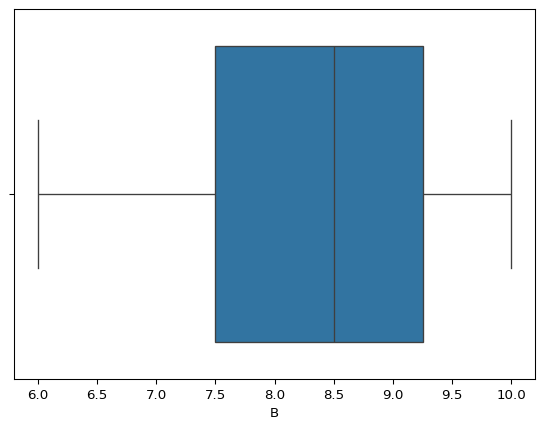
\includegraphics[keepaspectratio]{02-data-handling-exploration_files/figure-latex/cell-18-output-1.png}}

\pandocbounded{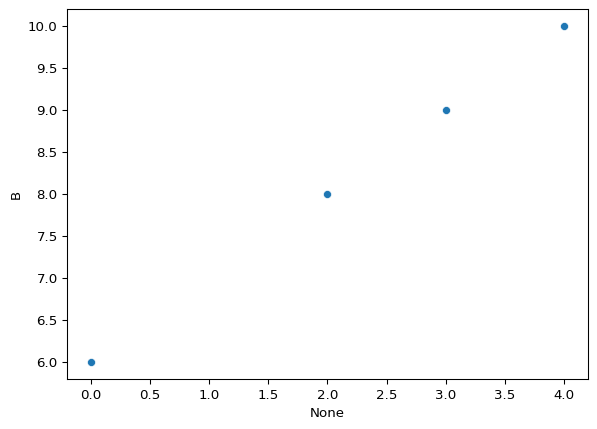
\includegraphics[keepaspectratio]{02-data-handling-exploration_files/figure-latex/cell-18-output-2.png}}

\begin{verbatim}
    * **통계적 방법:** Z-점수, 사분위 범위(Interquartile Range, IQR) 등을 사용하여 이상치를 탐지할 수 있습니다.
\end{verbatim}

\begin{Shaded}
\begin{Highlighting}[]
\NormalTok{    Q1 }\OperatorTok{=}\NormalTok{ df[}\StringTok{\textquotesingle{}B\textquotesingle{}}\NormalTok{].quantile(}\FloatTok{0.25}\NormalTok{)}
\NormalTok{    Q3 }\OperatorTok{=}\NormalTok{ df[}\StringTok{\textquotesingle{}B\textquotesingle{}}\NormalTok{].quantile(}\FloatTok{0.75}\NormalTok{)}
\NormalTok{    IQR }\OperatorTok{=}\NormalTok{ Q3 }\OperatorTok{{-}}\NormalTok{ Q1}
\NormalTok{    lower\_bound }\OperatorTok{=}\NormalTok{ Q1 }\OperatorTok{{-}} \FloatTok{1.5} \OperatorTok{*}\NormalTok{ IQR}
\NormalTok{    upper\_bound }\OperatorTok{=}\NormalTok{ Q3 }\OperatorTok{+} \FloatTok{1.5} \OperatorTok{*}\NormalTok{ IQR}
\NormalTok{    outliers }\OperatorTok{=}\NormalTok{ df[(df[}\StringTok{\textquotesingle{}B\textquotesingle{}}\NormalTok{] }\OperatorTok{\textless{}}\NormalTok{ lower\_bound) }\OperatorTok{|}\NormalTok{ (df[}\StringTok{\textquotesingle{}B\textquotesingle{}}\NormalTok{] }\OperatorTok{\textgreater{}}\NormalTok{ upper\_bound)]}
    \BuiltInTok{print}\NormalTok{(outliers)}
\end{Highlighting}
\end{Shaded}

\begin{verbatim}
Empty DataFrame
Columns: [A, B, C]
Index: []
\end{verbatim}

\begin{verbatim}
* **이상치 처리:**
    * **삭제:** 이상치를 포함하는 행 또는 열을 삭제합니다.
    * **대체:** 이상치를 특정 값(평균, 중앙값, 최빈값 등)으로 대체하거나, 상한/하한 값으로 제한합니다.
    * **변환:** 로그 변환, 제곱근 변환 등을 통해 이상치의 영향을 줄입니다.
\end{verbatim}

\begin{Shaded}
\begin{Highlighting}[]
\NormalTok{    df\_clipped }\OperatorTok{=}\NormalTok{ df.copy()}
\NormalTok{    df\_clipped[}\StringTok{\textquotesingle{}B\textquotesingle{}}\NormalTok{] }\OperatorTok{=}\NormalTok{ df\_clipped[}\StringTok{\textquotesingle{}B\textquotesingle{}}\NormalTok{].clip(lower}\OperatorTok{=}\NormalTok{lower\_bound, upper}\OperatorTok{=}\NormalTok{upper\_bound)}
    \BuiltInTok{print}\NormalTok{(df\_clipped)}
\end{Highlighting}
\end{Shaded}

\begin{verbatim}
     A     B     C
0  1.0   6.0     a
1  2.0   NaN     b
2  NaN   8.0     c
3  4.0   9.0  None
4  5.0  10.0     e
\end{verbatim}

\begin{verbatim}
|   처리 방법   |                       설명                       |                       예시                       |
| :-----------: | :--------------------------------------------: | :------------------------------------------------: |
|   이상치 탐지   |         시각적/통계적 방법으로 이상치 확인         |                   상자 그림, IQR                   |
|     삭제     |                 이상치를 포함하는 행/열 삭제                 |                 `df.dropna()`                 |
|     대체     |            이상치를 특정 값으로 대체/제한            |                   `df.fillna()`                   |
|     변환     |                로그 변환, 제곱근 변환 등                |                  `np.log()`                  |
\end{verbatim}

\subsection{2.2.3 변수 변환}\label{uxbcc0uxc218-uxbcc0uxd658}

\textbf{변수 변환(Variable Transformation)}은 변수의 형태나 분포를
변경하여 데이터 분석의 효율성을 높이거나, 특정 분석 방법에 적합하도록
데이터를 만드는 과정입니다.

\begin{itemize}
\item
  \textbf{(시각 자료 예시:} 변수 변환 방법을 보여주는 그림. 로그 변환,
  표준화, 정규화 등을 통해 변수의 분포나 척도를 변경하는 그림)

  \begin{itemize}
  \tightlist
  \item
    \textbf{척도 변환(Scaling):}

    \begin{itemize}
    \tightlist
    \item
      변수의 척도를 변경하여 서로 다른 변수 간의 비교를 용이하게 하거나,
      특정 알고리즘의 성능을 향상시킵니다.
    \item
      \textbf{표준화(Standardization):} 변수의 평균을 0, 표준편차를 1로
      변환합니다.
    \end{itemize}

    \(Z = \frac{X - \mu}{\sigma}\)
  \end{itemize}
\end{itemize}

\begin{Shaded}
\begin{Highlighting}[]
    \ImportTok{from}\NormalTok{ sklearn.preprocessing }\ImportTok{import}\NormalTok{ StandardScaler}

\NormalTok{    scaler }\OperatorTok{=}\NormalTok{ StandardScaler()}
\NormalTok{    df[}\StringTok{\textquotesingle{}A\_scaled\textquotesingle{}}\NormalTok{] }\OperatorTok{=}\NormalTok{ scaler.fit\_transform(df[[}\StringTok{\textquotesingle{}A\textquotesingle{}}\NormalTok{]])}
    \BuiltInTok{print}\NormalTok{(df[[}\StringTok{\textquotesingle{}A\textquotesingle{}}\NormalTok{, }\StringTok{\textquotesingle{}A\_scaled\textquotesingle{}}\NormalTok{]].head())}
\end{Highlighting}
\end{Shaded}

\begin{verbatim}
     A  A_scaled
0  1.0 -1.264911
1  2.0 -0.632456
2  NaN       NaN
3  4.0  0.632456
4  5.0  1.264911
\end{verbatim}

\begin{verbatim}
    * **정규화(Normalization):** 변수의 값을 0과 1 사이의 범위로 변환합니다.

    $X_{scaled} = \frac{X - X_{min}}{X_{max} - X_{min}}$
\end{verbatim}

\begin{Shaded}
\begin{Highlighting}[]
    \ImportTok{from}\NormalTok{ sklearn.preprocessing }\ImportTok{import}\NormalTok{ MinMaxScaler}

\NormalTok{    scaler }\OperatorTok{=}\NormalTok{ MinMaxScaler()}
\NormalTok{    df[}\StringTok{\textquotesingle{}B\_scaled\textquotesingle{}}\NormalTok{] }\OperatorTok{=}\NormalTok{ scaler.fit\_transform(df[[}\StringTok{\textquotesingle{}B\textquotesingle{}}\NormalTok{]])}
    \BuiltInTok{print}\NormalTok{(df[[}\StringTok{\textquotesingle{}B\textquotesingle{}}\NormalTok{, }\StringTok{\textquotesingle{}B\_scaled\textquotesingle{}}\NormalTok{]].head())}
\end{Highlighting}
\end{Shaded}

\begin{verbatim}
      B  B_scaled
0   6.0      0.00
1   NaN       NaN
2   8.0      0.50
3   9.0      0.75
4  10.0      1.00
\end{verbatim}

\begin{verbatim}
* **분포 변환(Distribution Transformation):**
    * 변수의 분포를 변경하여 특정 분석 방법에 적합하도록 만듭니다.
    * **로그 변환(Log Transformation):** 오른쪽으로 꼬리가 긴 분포(Right-Skewed Distribution)를 정규 분포에 가깝게 만듭니다.
\end{verbatim}

\begin{Shaded}
\begin{Highlighting}[]
    \ImportTok{import}\NormalTok{ numpy }\ImportTok{as}\NormalTok{ np}

\NormalTok{    df\_log }\OperatorTok{=}\NormalTok{ df.copy()}
\NormalTok{    df\_log[}\StringTok{\textquotesingle{}A\_log\textquotesingle{}}\NormalTok{] }\OperatorTok{=}\NormalTok{ np.log(df\_log[}\StringTok{\textquotesingle{}A\textquotesingle{}}\NormalTok{][df\_log[}\StringTok{\textquotesingle{}A\textquotesingle{}}\NormalTok{] }\OperatorTok{\textgreater{}} \DecValTok{0}\NormalTok{]) }\CommentTok{\# 0 또는 음수 값을 제외하고 로그 변환}
    \BuiltInTok{print}\NormalTok{(df\_log[[}\StringTok{\textquotesingle{}A\textquotesingle{}}\NormalTok{, }\StringTok{\textquotesingle{}A\_log\textquotesingle{}}\NormalTok{]].head())}
\end{Highlighting}
\end{Shaded}

\begin{verbatim}
     A     A_log
0  1.0  0.000000
1  2.0  0.693147
2  NaN       NaN
3  4.0  1.386294
4  5.0  1.609438
\end{verbatim}

\begin{verbatim}
    * **제곱근 변환(Square Root Transformation):** 로그 변환과 유사한 효과를 가지며, 0을 포함하는 데이터에 적용할 수 있습니다.
\end{verbatim}

\begin{Shaded}
\begin{Highlighting}[]
\NormalTok{    df\_sqrt }\OperatorTok{=}\NormalTok{ df.copy()}
\NormalTok{    df\_sqrt[}\StringTok{\textquotesingle{}B\_sqrt\textquotesingle{}}\NormalTok{] }\OperatorTok{=}\NormalTok{ np.sqrt(df\_sqrt[}\StringTok{\textquotesingle{}B\textquotesingle{}}\NormalTok{][df\_sqrt[}\StringTok{\textquotesingle{}B\textquotesingle{}}\NormalTok{] }\OperatorTok{\textgreater{}=} \DecValTok{0}\NormalTok{]) }\CommentTok{\# 음수 값을 제외하고 제곱근 변환}
    \BuiltInTok{print}\NormalTok{(df\_sqrt[[}\StringTok{\textquotesingle{}B\textquotesingle{}}\NormalTok{, }\StringTok{\textquotesingle{}B\_sqrt\textquotesingle{}}\NormalTok{]].head())}
\end{Highlighting}
\end{Shaded}

\begin{verbatim}
      B    B_sqrt
0   6.0  2.449490
1   NaN       NaN
2   8.0  2.828427
3   9.0  3.000000
4  10.0  3.162278
\end{verbatim}

\begin{verbatim}
* **범주형 변수 처리:**
    * 범주형 변수를 분석에 활용하기 위해 수치형 변수로 변환합니다.
    * **더미 변수화(Dummy Variable Encoding):** 각 범주를 0 또는 1로 표현하는 새로운 변수를 생성합니다.
\end{verbatim}

\begin{Shaded}
\begin{Highlighting}[]
\NormalTok{    df\_encoded }\OperatorTok{=}\NormalTok{ pd.get\_dummies(df, columns}\OperatorTok{=}\NormalTok{[}\StringTok{\textquotesingle{}C\textquotesingle{}}\NormalTok{], drop\_first}\OperatorTok{=}\VariableTok{True}\NormalTok{) }\CommentTok{\# \textquotesingle{}C\textquotesingle{} 열을 더미 변수화 (첫 번째 범주 제외)}
    \BuiltInTok{print}\NormalTok{(df\_encoded.head())}
\end{Highlighting}
\end{Shaded}

\begin{verbatim}
     A     B  A_scaled  B_scaled    C_b    C_c    C_e
0  1.0   6.0 -1.264911      0.00  False  False  False
1  2.0   NaN -0.632456       NaN   True  False  False
2  NaN   8.0       NaN      0.50  False   True  False
3  4.0   9.0  0.632456      0.75  False  False  False
4  5.0  10.0  1.264911      1.00  False  False   True
\end{verbatim}

\begin{verbatim}
    * **원-핫 인코딩(One-Hot Encoding):** 더미 변수화와 유사하지만, 첫 번째 범주를 제외하지 않습니다.
\end{verbatim}

\begin{Shaded}
\begin{Highlighting}[]
\NormalTok{    df\_onehot }\OperatorTok{=}\NormalTok{ pd.get\_dummies(df, columns}\OperatorTok{=}\NormalTok{[}\StringTok{\textquotesingle{}C\textquotesingle{}}\NormalTok{]) }\CommentTok{\# \textquotesingle{}C\textquotesingle{} 열을 원{-}핫 인코딩}
    \BuiltInTok{print}\NormalTok{(df\_onehot.head())}
\end{Highlighting}
\end{Shaded}

\begin{verbatim}
     A     B  A_scaled  B_scaled    C_a    C_b    C_c    C_e
0  1.0   6.0 -1.264911      0.00   True  False  False  False
1  2.0   NaN -0.632456       NaN  False   True  False  False
2  NaN   8.0       NaN      0.50  False  False   True  False
3  4.0   9.0  0.632456      0.75  False  False  False  False
4  5.0  10.0  1.264911      1.00  False  False  False   True
\end{verbatim}

\begin{verbatim}
|   변환 방법   |                       설명                       |                       예시                       |
| :-----------: | :--------------------------------------------: | :------------------------------------------------: |
|   척도 변환   |               변수의 척도를 변경               |         표준화, 정규화         |
|   분포 변환   |               변수의 분포를 변경               |         로그 변환, 제곱근 변환         |
| 범주형 변수 처리 |             범주형 변수를 수치형으로 변환             | 더미 변수화, 원-핫 인코딩 |
\end{verbatim}

\subsection{2.2.4 데이터 전처리 과정의
중요성}\label{uxb370uxc774uxd130-uxc804uxcc98uxb9ac-uxacfcuxc815uxc758-uxc911uxc694uxc131}

데이터 전처리는 데이터 분석의 정확성과 신뢰성을 높이는 데 필수적인
과정입니다. 적절한 전처리 과정을 통해 데이터의 품질을 향상시키고, 분석에
적합한 형태로 데이터를 변환함으로써, 연구자는 더욱 정확하고 의미 있는
결과를 얻을 수 있습니다.

\section{2.3 기술 통계 분석}\label{sec-descriptive-stats}

데이터 전처리를 통해 데이터를 분석에 적합한 형태로 정제했다면, 다음
단계는 데이터의 기본적인 특성을 파악하는 것입니다. \textbf{기술 통계
분석(Descriptive Statistics Analysis)}은 수집된 데이터를 요약하고
설명하여 데이터가 가진 정보를 효과적으로 전달하는 통계적 방법입니다.
이는 데이터의 중심 경향성(Central Tendency), 산포도(Dispersion), 분포
형태(Distribution Shape) 등을 파악하여 데이터에 대한 깊이 있는 이해를
돕고, 이어질 추론 통계 분석의 기초를 마련합니다.

본 절에서는 파이썬 Pandas 라이브러리를 활용하여 주요 기술 통계량을
계산하고 해석하는 방법을 학습합니다.

\begin{tcolorbox}[enhanced jigsaw, bottomtitle=1mm, colbacktitle=quarto-callout-note-color!10!white, rightrule=.15mm, colback=white, leftrule=.75mm, toptitle=1mm, titlerule=0mm, opacityback=0, opacitybacktitle=0.6, left=2mm, title=\textcolor{quarto-callout-note-color}{\faInfo}\hspace{0.5em}{📌 핵심 요약}, breakable, bottomrule=.15mm, arc=.35mm, colframe=quarto-callout-note-color-frame, toprule=.15mm, coltitle=black]

기술 통계 분석은 데이터의 기본적인 특성을 요약하고 설명하는 과정입니다.
Pandas를 이용하여 평균, 중앙값, 최빈값 등 중심 경향성 지표와 분산,
표준편차, 범위, 사분위수 등 산포도 지표를 계산하고 해석하는 방법을
배웁니다. 또한, 범주형 데이터의 빈도 분석 방법과 \texttt{.describe()}
함수를 활용한 요약 통계량 확인 방법을 익힙니다.

\end{tcolorbox}

\emph{(시각 자료 예시: 기술 통계 분석의 주요 목표(중심 경향성, 산포도,
분포 형태 파악)를 보여주는 다이어그램)}

\subsection{가상 데이터
생성}\label{uxac00uxc0c1-uxb370uxc774uxd130-uxc0dduxc131}

기술 통계 분석 실습을 위해 가상의 설문조사 응답 데이터를 담은 Pandas
DataFrame을 생성해 보겠습니다. 이 데이터는 `ID', `Age', `Gender',
`EducationLevel', `SatisfactionScore', `Income' 열을 포함합니다.

\begin{Shaded}
\begin{Highlighting}[]
\ImportTok{import}\NormalTok{ pandas }\ImportTok{as}\NormalTok{ pd}
\ImportTok{import}\NormalTok{ numpy }\ImportTok{as}\NormalTok{ np}

\CommentTok{\# 가상 데이터 생성}
\NormalTok{data }\OperatorTok{=}\NormalTok{ \{}
    \StringTok{\textquotesingle{}ID\textquotesingle{}}\NormalTok{: }\BuiltInTok{range}\NormalTok{(}\DecValTok{1}\NormalTok{, }\DecValTok{11}\NormalTok{),}
    \StringTok{\textquotesingle{}Age\textquotesingle{}}\NormalTok{: [}\DecValTok{25}\NormalTok{, }\DecValTok{30}\NormalTok{, }\DecValTok{28}\NormalTok{, }\DecValTok{35}\NormalTok{, }\DecValTok{42}\NormalTok{, }\DecValTok{29}\NormalTok{, }\DecValTok{31}\NormalTok{, }\DecValTok{45}\NormalTok{, }\DecValTok{22}\NormalTok{, }\DecValTok{38}\NormalTok{],}
    \StringTok{\textquotesingle{}Gender\textquotesingle{}}\NormalTok{: [}\StringTok{\textquotesingle{}Female\textquotesingle{}}\NormalTok{, }\StringTok{\textquotesingle{}Male\textquotesingle{}}\NormalTok{, }\StringTok{\textquotesingle{}Male\textquotesingle{}}\NormalTok{, }\StringTok{\textquotesingle{}Female\textquotesingle{}}\NormalTok{, }\StringTok{\textquotesingle{}Male\textquotesingle{}}\NormalTok{, }\StringTok{\textquotesingle{}Female\textquotesingle{}}\NormalTok{, }\StringTok{\textquotesingle{}Male\textquotesingle{}}\NormalTok{, }\StringTok{\textquotesingle{}Female\textquotesingle{}}\NormalTok{, }\StringTok{\textquotesingle{}Female\textquotesingle{}}\NormalTok{, }\StringTok{\textquotesingle{}Male\textquotesingle{}}\NormalTok{],}
    \StringTok{\textquotesingle{}EducationLevel\textquotesingle{}}\NormalTok{: [}\StringTok{\textquotesingle{}Bachelor\textquotesingle{}}\NormalTok{, }\StringTok{\textquotesingle{}Master\textquotesingle{}}\NormalTok{, }\StringTok{\textquotesingle{}Bachelor\textquotesingle{}}\NormalTok{, }\StringTok{\textquotesingle{}PhD\textquotesingle{}}\NormalTok{, }\StringTok{\textquotesingle{}Master\textquotesingle{}}\NormalTok{, }\StringTok{\textquotesingle{}Bachelor\textquotesingle{}}\NormalTok{, }\StringTok{\textquotesingle{}Master\textquotesingle{}}\NormalTok{, }\StringTok{\textquotesingle{}PhD\textquotesingle{}}\NormalTok{, }\StringTok{\textquotesingle{}High School\textquotesingle{}}\NormalTok{, }\StringTok{\textquotesingle{}Master\textquotesingle{}}\NormalTok{],}
    \StringTok{\textquotesingle{}SatisfactionScore\textquotesingle{}}\NormalTok{: [}\DecValTok{7}\NormalTok{, }\DecValTok{8}\NormalTok{, }\DecValTok{6}\NormalTok{, }\DecValTok{9}\NormalTok{, }\DecValTok{7}\NormalTok{, np.nan, }\DecValTok{8}\NormalTok{, }\DecValTok{10}\NormalTok{, }\DecValTok{5}\NormalTok{, }\DecValTok{7}\NormalTok{], }\CommentTok{\# 결측치(NaN) 포함}
    \StringTok{\textquotesingle{}Income\textquotesingle{}}\NormalTok{: [}\DecValTok{5000}\NormalTok{, }\DecValTok{6000}\NormalTok{, }\DecValTok{5500}\NormalTok{, }\DecValTok{7500}\NormalTok{, }\DecValTok{8000}\NormalTok{, }\DecValTok{5200}\NormalTok{, }\DecValTok{6100}\NormalTok{, }\DecValTok{9000}\NormalTok{, }\DecValTok{4000}\NormalTok{, }\DecValTok{7000}\NormalTok{]}
\NormalTok{\}}
\NormalTok{df\_survey }\OperatorTok{=}\NormalTok{ pd.DataFrame(data)}

\BuiltInTok{print}\NormalTok{(}\StringTok{"가상 설문조사 데이터:"}\NormalTok{)}
\BuiltInTok{print}\NormalTok{(df\_survey.head()) }\CommentTok{\# 데이터 일부 확인}
\BuiltInTok{print}\NormalTok{(}\StringTok{"}\CharTok{\textbackslash{}n}\StringTok{데이터 정보 요약:"}\NormalTok{)}
\BuiltInTok{print}\NormalTok{(df\_survey.info()) }\CommentTok{\# 데이터 구조 및 결측치 확인}
\end{Highlighting}
\end{Shaded}

\begin{verbatim}
가상 설문조사 데이터:
   ID  Age  Gender EducationLevel  SatisfactionScore  Income
0   1   25  Female       Bachelor                7.0    5000
1   2   30    Male         Master                8.0    6000
2   3   28    Male       Bachelor                6.0    5500
3   4   35  Female            PhD                9.0    7500
4   5   42    Male         Master                7.0    8000

데이터 정보 요약:
<class 'pandas.core.frame.DataFrame'>
RangeIndex: 10 entries, 0 to 9
Data columns (total 6 columns):
 #   Column             Non-Null Count  Dtype  
---  ------             --------------  -----  
 0   ID                 10 non-null     int64  
 1   Age                10 non-null     int64  
 2   Gender             10 non-null     object 
 3   EducationLevel     10 non-null     object 
 4   SatisfactionScore  9 non-null      float64
 5   Income             10 non-null     int64  
dtypes: float64(1), int64(3), object(2)
memory usage: 612.0+ bytes
None
\end{verbatim}

\textbf{참고:} Pandas의 대부분 기술 통계 함수는 기본적으로
결측치(\texttt{NaN})를 제외하고 계산합니다. 이는 \texttt{skipna=True}
(기본값) 설정 때문입니다.

\subsection{2.3.1 중심 경향성 측정 (Measures of Central
Tendency)}\label{uxc911uxc2ec-uxacbduxd5a5uxc131-uxce21uxc815-measures-of-central-tendency}

데이터의 중심 경향성은 데이터 값들이 어떤 값을 중심으로 분포하는 경향이
있는지를 나타내는 척도입니다. 대표적인 중심 경향성 측정 지표로는 평균,
중앙값, 최빈값이 있습니다.

\begin{itemize}
\item
  \textbf{(시각 자료 예시:} 정규분포 곡선 위에 평균, 중앙값, 최빈값이
  일치하는 모습을 보여주고, 비대칭 분포(skewed distribution)에서 세 값이
  달라지는 모습을 비교하는 그림)
\item
  \textbf{평균 (Mean):}

  \begin{itemize}
  \tightlist
  \item
    모든 데이터 값을 더한 후 데이터 개수로 나눈 값입니다.
  \item
    데이터 전체의 값을 반영하지만, 극단적인 값(이상치)에 영향을 받기
    쉽습니다.
  \item
    Pandas에서는 \texttt{.mean()} 메서드를 사용합니다.
  \end{itemize}
\end{itemize}

\begin{Shaded}
\begin{Highlighting}[]
    \CommentTok{\# Age와 Income 열의 평균 계산}
\NormalTok{    mean\_age }\OperatorTok{=}\NormalTok{ df\_survey[}\StringTok{\textquotesingle{}Age\textquotesingle{}}\NormalTok{].mean()}
\NormalTok{    mean\_income }\OperatorTok{=}\NormalTok{ df\_survey[}\StringTok{\textquotesingle{}Income\textquotesingle{}}\NormalTok{].mean()}
\NormalTok{    mean\_satisfaction }\OperatorTok{=}\NormalTok{ df\_survey[}\StringTok{\textquotesingle{}SatisfactionScore\textquotesingle{}}\NormalTok{].mean() }\CommentTok{\# NaN은 자동 제외}

    \BuiltInTok{print}\NormalTok{(}\SpecialStringTok{f"평균 나이: }\SpecialCharTok{\{}\NormalTok{mean\_age}\SpecialCharTok{:.2f\}}\SpecialStringTok{"}\NormalTok{)}
    \BuiltInTok{print}\NormalTok{(}\SpecialStringTok{f"평균 소득: }\SpecialCharTok{\{}\NormalTok{mean\_income}\SpecialCharTok{:.2f\}}\SpecialStringTok{"}\NormalTok{)}
    \BuiltInTok{print}\NormalTok{(}\SpecialStringTok{f"평균 만족도 점수: }\SpecialCharTok{\{}\NormalTok{mean\_satisfaction}\SpecialCharTok{:.2f\}}\SpecialStringTok{"}\NormalTok{)}
\end{Highlighting}
\end{Shaded}

\begin{verbatim}
평균 나이: 32.50
평균 소득: 6330.00
평균 만족도 점수: 7.44
\end{verbatim}

\begin{itemize}
\tightlist
\item
  \textbf{중앙값 (Median):}

  \begin{itemize}
  \tightlist
  \item
    데이터를 크기 순서대로 정렬했을 때 중앙에 위치하는 값입니다.
  \item
    데이터 개수가 짝수일 경우, 중앙에 위치한 두 값의 평균을 사용합니다.
  \item
    평균과 달리 극단적인 값(이상치)에 영향을 덜 받습니다 (Robust).
  \item
    Pandas에서는 \texttt{.median()} 메서드를 사용합니다.
  \end{itemize}
\end{itemize}

\begin{Shaded}
\begin{Highlighting}[]
    \CommentTok{\# Age와 Income 열의 중앙값 계산}
\NormalTok{    median\_age }\OperatorTok{=}\NormalTok{ df\_survey[}\StringTok{\textquotesingle{}Age\textquotesingle{}}\NormalTok{].median()}
\NormalTok{    median\_income }\OperatorTok{=}\NormalTok{ df\_survey[}\StringTok{\textquotesingle{}Income\textquotesingle{}}\NormalTok{].median()}
\NormalTok{    median\_satisfaction }\OperatorTok{=}\NormalTok{ df\_survey[}\StringTok{\textquotesingle{}SatisfactionScore\textquotesingle{}}\NormalTok{].median() }\CommentTok{\# NaN은 자동 제외}

    \BuiltInTok{print}\NormalTok{(}\SpecialStringTok{f"나이 중앙값: }\SpecialCharTok{\{}\NormalTok{median\_age}\SpecialCharTok{\}}\SpecialStringTok{"}\NormalTok{)}
    \BuiltInTok{print}\NormalTok{(}\SpecialStringTok{f"소득 중앙값: }\SpecialCharTok{\{}\NormalTok{median\_income}\SpecialCharTok{\}}\SpecialStringTok{"}\NormalTok{)}
    \BuiltInTok{print}\NormalTok{(}\SpecialStringTok{f"만족도 점수 중앙값: }\SpecialCharTok{\{}\NormalTok{median\_satisfaction}\SpecialCharTok{\}}\SpecialStringTok{"}\NormalTok{)}

    \CommentTok{\# 평균과 중앙값 비교 (소득 분포가 비대칭적일 경우 차이가 발생할 수 있음)}
    \BuiltInTok{print}\NormalTok{(}\SpecialStringTok{f"}\CharTok{\textbackslash{}n}\SpecialStringTok{소득 {-} 평균: }\SpecialCharTok{\{}\NormalTok{mean\_income}\SpecialCharTok{:.2f\}}\SpecialStringTok{, 중앙값: }\SpecialCharTok{\{}\NormalTok{median\_income}\SpecialCharTok{\}}\SpecialStringTok{"}\NormalTok{)}
\end{Highlighting}
\end{Shaded}

\begin{verbatim}
나이 중앙값: 30.5
소득 중앙값: 6050.0
만족도 점수 중앙값: 7.0

소득 - 평균: 6330.00, 중앙값: 6050.0
\end{verbatim}

\begin{itemize}
\tightlist
\item
  \textbf{최빈값 (Mode):}

  \begin{itemize}
  \tightlist
  \item
    데이터에서 가장 빈번하게 나타나는 값입니다.
  \item
    연속형 데이터보다는 범주형 데이터나 이산형 데이터에서 주로
    사용됩니다.
  \item
    최빈값은 여러 개 존재할 수 있습니다.
  \item
    Pandas에서는 \texttt{.mode()} 메서드를 사용합니다.
    \texttt{.mode()}는 최빈값이 여러 개일 경우 모든 값을 Series 형태로
    반환합니다.
  \end{itemize}
\end{itemize}

\begin{Shaded}
\begin{Highlighting}[]
    \CommentTok{\# Gender와 EducationLevel 열의 최빈값 계산}
\NormalTok{    mode\_gender }\OperatorTok{=}\NormalTok{ df\_survey[}\StringTok{\textquotesingle{}Gender\textquotesingle{}}\NormalTok{].mode()}
\NormalTok{    mode\_education }\OperatorTok{=}\NormalTok{ df\_survey[}\StringTok{\textquotesingle{}EducationLevel\textquotesingle{}}\NormalTok{].mode()}
\NormalTok{    mode\_satisfaction }\OperatorTok{=}\NormalTok{ df\_survey[}\StringTok{\textquotesingle{}SatisfactionScore\textquotesingle{}}\NormalTok{].mode() }\CommentTok{\# 최빈값은 여러 개일 수 있음}

    \BuiltInTok{print}\NormalTok{(}\SpecialStringTok{f"성별 최빈값:}\CharTok{\textbackslash{}n}\SpecialCharTok{\{}\NormalTok{mode\_gender}\SpecialCharTok{\}}\SpecialStringTok{"}\NormalTok{)}
    \BuiltInTok{print}\NormalTok{(}\SpecialStringTok{f"}\CharTok{\textbackslash{}n}\SpecialStringTok{학력 최빈값:}\CharTok{\textbackslash{}n}\SpecialCharTok{\{}\NormalTok{mode\_education}\SpecialCharTok{\}}\SpecialStringTok{"}\NormalTok{)}
    \BuiltInTok{print}\NormalTok{(}\SpecialStringTok{f"}\CharTok{\textbackslash{}n}\SpecialStringTok{만족도 점수 최빈값:}\CharTok{\textbackslash{}n}\SpecialCharTok{\{}\NormalTok{mode\_satisfaction}\SpecialCharTok{\}}\SpecialStringTok{"}\NormalTok{) }\CommentTok{\# 7점이 3번으로 가장 많음}
\end{Highlighting}
\end{Shaded}

\begin{verbatim}
성별 최빈값:
0    Female
1      Male
Name: Gender, dtype: object

학력 최빈값:
0    Master
Name: EducationLevel, dtype: object

만족도 점수 최빈값:
0    7.0
Name: SatisfactionScore, dtype: float64
\end{verbatim}

\begin{longtable}[]{@{}
  >{\raggedright\arraybackslash}p{(\linewidth - 6\tabcolsep) * \real{0.1176}}
  >{\raggedright\arraybackslash}p{(\linewidth - 6\tabcolsep) * \real{0.4000}}
  >{\raggedright\arraybackslash}p{(\linewidth - 6\tabcolsep) * \real{0.1529}}
  >{\raggedright\arraybackslash}p{(\linewidth - 6\tabcolsep) * \real{0.3294}}@{}}
\toprule\noalign{}
\begin{minipage}[b]{\linewidth}\raggedright
측정 지표
\end{minipage} & \begin{minipage}[b]{\linewidth}\raggedright
설명
\end{minipage} & \begin{minipage}[b]{\linewidth}\raggedright
Pandas 메서드
\end{minipage} & \begin{minipage}[b]{\linewidth}\raggedright
특징
\end{minipage} \\
\midrule\noalign{}
\endhead
\bottomrule\noalign{}
\endlastfoot
평균 (Mean) & 모든 값의 합 / 개수 & \texttt{.mean()} & 이상치에 민감 \\
중앙값 (Median) & 정렬 시 중앙에 위치하는 값 & \texttt{.median()} &
이상치에 덜 민감 (Robust) \\
최빈값 (Mode) & 가장 빈번하게 나타나는 값 & \texttt{.mode()} & 범주형
데이터에 유용, 여러 개 가능 \\
\end{longtable}

\subsection{2.3.2 산포도 측정 (Measures of
Dispersion)}\label{uxc0b0uxd3ecuxb3c4-uxce21uxc815-measures-of-dispersion}

산포도는 데이터 값들이 중심 경향성 값(주로 평균)으로부터 얼마나 흩어져
있는지를 나타내는 척도입니다. 데이터의 변동성이나 다양성을 파악하는 데
중요합니다.

\begin{itemize}
\item
  \textbf{(시각 자료 예시:} 평균은 같지만 분산(표준편차)이 다른 두
  분포를 비교하는 그림. 좁고 뾰족한 분포와 넓고 평평한 분포)
\item
  \textbf{범위 (Range):}

  \begin{itemize}
  \tightlist
  \item
    데이터의 최댓값과 최솟값의 차이입니다.
  \item
    계산이 간단하지만, 양 극단의 값에만 의존하므로 데이터 전체의 흩어짐
    정도를 충분히 반영하지 못할 수 있습니다.
  \item
    Pandas에서는 \texttt{.max()}와 \texttt{.min()}을 이용하여
    계산합니다.
  \end{itemize}
\end{itemize}

\begin{Shaded}
\begin{Highlighting}[]
    \CommentTok{\# Age의 범위 계산}
\NormalTok{    range\_age }\OperatorTok{=}\NormalTok{ df\_survey[}\StringTok{\textquotesingle{}Age\textquotesingle{}}\NormalTok{].}\BuiltInTok{max}\NormalTok{() }\OperatorTok{{-}}\NormalTok{ df\_survey[}\StringTok{\textquotesingle{}Age\textquotesingle{}}\NormalTok{].}\BuiltInTok{min}\NormalTok{()}
    \BuiltInTok{print}\NormalTok{(}\SpecialStringTok{f"나이 범위: }\SpecialCharTok{\{}\NormalTok{range\_age}\SpecialCharTok{\}}\SpecialStringTok{ (최소: }\SpecialCharTok{\{}\NormalTok{df\_survey[}\StringTok{\textquotesingle{}Age\textquotesingle{}}\NormalTok{]}\SpecialCharTok{.}\BuiltInTok{min}\NormalTok{()}\SpecialCharTok{\}}\SpecialStringTok{, 최대: }\SpecialCharTok{\{}\NormalTok{df\_survey[}\StringTok{\textquotesingle{}Age\textquotesingle{}}\NormalTok{]}\SpecialCharTok{.}\BuiltInTok{max}\NormalTok{()}\SpecialCharTok{\}}\SpecialStringTok{)"}\NormalTok{)}
\end{Highlighting}
\end{Shaded}

\begin{verbatim}
나이 범위: 23 (최소: 22, 최대: 45)
\end{verbatim}

\begin{itemize}
\tightlist
\item
  \textbf{분산 (Variance) 및 표준편차 (Standard Deviation):}

  \begin{itemize}
  \tightlist
  \item
    \textbf{분산:} 각 데이터 값이 평균으로부터 얼마나 떨어져
    있는지(편차)를 제곱하여 평균 낸 값입니다. 데이터의 퍼짐 정도를
    나타냅니다. 단위가 원래 데이터 단위의 제곱이 됩니다.
  \item
    \textbf{표준편차:} 분산에 제곱근을 취한 값입니다. 분산과 동일하게
    데이터의 퍼짐 정도를 나타내지만, 단위가 원래 데이터와 동일하여
    해석이 용이합니다.
  \item
    Pandas에서는 \texttt{.var()} (분산)와 \texttt{.std()} (표준편차)
    메서드를 사용합니다. 기본적으로 표본 분산/표준편차 (n-1로 나눔,
    \texttt{ddof=1})를 계산합니다.
  \end{itemize}
\end{itemize}

\begin{Shaded}
\begin{Highlighting}[]
    \CommentTok{\# Age와 Income의 분산 및 표준편차 계산}
\NormalTok{    var\_age }\OperatorTok{=}\NormalTok{ df\_survey[}\StringTok{\textquotesingle{}Age\textquotesingle{}}\NormalTok{].var()}
\NormalTok{    std\_age }\OperatorTok{=}\NormalTok{ df\_survey[}\StringTok{\textquotesingle{}Age\textquotesingle{}}\NormalTok{].std()}
\NormalTok{    var\_income }\OperatorTok{=}\NormalTok{ df\_survey[}\StringTok{\textquotesingle{}Income\textquotesingle{}}\NormalTok{].var()}
\NormalTok{    std\_income }\OperatorTok{=}\NormalTok{ df\_survey[}\StringTok{\textquotesingle{}Income\textquotesingle{}}\NormalTok{].std()}
\NormalTok{    std\_satisfaction }\OperatorTok{=}\NormalTok{ df\_survey[}\StringTok{\textquotesingle{}SatisfactionScore\textquotesingle{}}\NormalTok{].std()}

    \BuiltInTok{print}\NormalTok{(}\SpecialStringTok{f"나이 분산: }\SpecialCharTok{\{}\NormalTok{var\_age}\SpecialCharTok{:.2f\}}\SpecialStringTok{, 표준편차: }\SpecialCharTok{\{}\NormalTok{std\_age}\SpecialCharTok{:.2f\}}\SpecialStringTok{"}\NormalTok{)}
    \BuiltInTok{print}\NormalTok{(}\SpecialStringTok{f"소득 분산: }\SpecialCharTok{\{}\NormalTok{var\_income}\SpecialCharTok{:.2f\}}\SpecialStringTok{, 표준편차: }\SpecialCharTok{\{}\NormalTok{std\_income}\SpecialCharTok{:.2f\}}\SpecialStringTok{"}\NormalTok{)}
    \BuiltInTok{print}\NormalTok{(}\SpecialStringTok{f"만족도 점수 표준편차: }\SpecialCharTok{\{}\NormalTok{std\_satisfaction}\SpecialCharTok{:.2f\}}\SpecialStringTok{"}\NormalTok{)}
\end{Highlighting}
\end{Shaded}

\begin{verbatim}
나이 분산: 54.50, 표준편차: 7.38
소득 분산: 2340111.11, 표준편차: 1529.74
만족도 점수 표준편차: 1.51
\end{verbatim}

\begin{itemize}
\tightlist
\item
  \textbf{사분위수 (Quartiles) 및 사분위 범위 (Interquartile Range,
  IQR):}

  \begin{itemize}
  \tightlist
  \item
    \textbf{사분위수:} 데이터를 크기 순으로 정렬했을 때, 4등분하는
    위치에 있는 값입니다.

    \begin{itemize}
    \tightlist
    \item
      제1사분위수 (Q1): 하위 25\% 지점의 값
    \item
      제2사분위수 (Q2): 50\% 지점의 값 (중앙값과 동일)
    \item
      제3사분위수 (Q3): 하위 75\% 지점의 값
    \end{itemize}
  \item
    \textbf{사분위 범위 (IQR):} 제3사분위수(Q3)와 제1사분위수(Q1)의 차이
    (IQR = Q3 - Q1)입니다. 데이터의 중간 50\%가 분포하는 범위이며,
    이상치 탐지에도 활용됩니다 (2.2.2절 참고).
  \item
    Pandas에서는 \texttt{.quantile()} 메서드를 사용하여 특정 분위수를
    계산할 수 있습니다. (예:
    \texttt{df{[}\textquotesingle{}col\textquotesingle{}{]}.quantile(0.25)}는
    Q1)
  \end{itemize}
\end{itemize}

\begin{Shaded}
\begin{Highlighting}[]
    \CommentTok{\# Income의 사분위수 및 IQR 계산}
\NormalTok{    Q1\_income }\OperatorTok{=}\NormalTok{ df\_survey[}\StringTok{\textquotesingle{}Income\textquotesingle{}}\NormalTok{].quantile(}\FloatTok{0.25}\NormalTok{)}
\NormalTok{    Q2\_income }\OperatorTok{=}\NormalTok{ df\_survey[}\StringTok{\textquotesingle{}Income\textquotesingle{}}\NormalTok{].quantile(}\FloatTok{0.50}\NormalTok{) }\CommentTok{\# 중앙값과 동일}
\NormalTok{    Q3\_income }\OperatorTok{=}\NormalTok{ df\_survey[}\StringTok{\textquotesingle{}Income\textquotesingle{}}\NormalTok{].quantile(}\FloatTok{0.75}\NormalTok{)}
\NormalTok{    IQR\_income }\OperatorTok{=}\NormalTok{ Q3\_income }\OperatorTok{{-}}\NormalTok{ Q1\_income}

    \BuiltInTok{print}\NormalTok{(}\SpecialStringTok{f"소득 제1사분위수 (Q1): }\SpecialCharTok{\{}\NormalTok{Q1\_income}\SpecialCharTok{\}}\SpecialStringTok{"}\NormalTok{)}
    \BuiltInTok{print}\NormalTok{(}\SpecialStringTok{f"소득 제2사분위수 (Q2/Median): }\SpecialCharTok{\{}\NormalTok{Q2\_income}\SpecialCharTok{\}}\SpecialStringTok{"}\NormalTok{)}
    \BuiltInTok{print}\NormalTok{(}\SpecialStringTok{f"소득 제3사분위수 (Q3): }\SpecialCharTok{\{}\NormalTok{Q3\_income}\SpecialCharTok{\}}\SpecialStringTok{"}\NormalTok{)}
    \BuiltInTok{print}\NormalTok{(}\SpecialStringTok{f"소득 사분위 범위 (IQR): }\SpecialCharTok{\{}\NormalTok{IQR\_income}\SpecialCharTok{\}}\SpecialStringTok{"}\NormalTok{)}
\end{Highlighting}
\end{Shaded}

\begin{verbatim}
소득 제1사분위수 (Q1): 5275.0
소득 제2사분위수 (Q2/Median): 6050.0
소득 제3사분위수 (Q3): 7375.0
소득 사분위 범위 (IQR): 2100.0
\end{verbatim}

\begin{longtable}[]{@{}
  >{\raggedright\arraybackslash}p{(\linewidth - 6\tabcolsep) * \real{0.1356}}
  >{\raggedright\arraybackslash}p{(\linewidth - 6\tabcolsep) * \real{0.3220}}
  >{\raggedright\arraybackslash}p{(\linewidth - 6\tabcolsep) * \real{0.2542}}
  >{\raggedright\arraybackslash}p{(\linewidth - 6\tabcolsep) * \real{0.2881}}@{}}
\toprule\noalign{}
\begin{minipage}[b]{\linewidth}\raggedright
측정 지표
\end{minipage} & \begin{minipage}[b]{\linewidth}\raggedright
설명
\end{minipage} & \begin{minipage}[b]{\linewidth}\raggedright
Pandas 메서드 / 계산
\end{minipage} & \begin{minipage}[b]{\linewidth}\raggedright
특징
\end{minipage} \\
\midrule\noalign{}
\endhead
\bottomrule\noalign{}
\endlastfoot
범위 (Range) & 최댓값 - 최솟값 & \texttt{.max()} - \texttt{.min()} &
계산 간편, 이상치에 민감 \\
분산 (Variance) & 편차 제곱의 평균 & \texttt{.var()} & 퍼짐 정도 측정,
단위가 제곱됨 \\
표준편차 (Std Dev) & 분산의 제곱근 & \texttt{.std()} & 퍼짐 정도 측정,
원래 단위와 동일 \\
사분위수 (Quartile) & 데이터를 4등분하는 지점의 값 &
\texttt{.quantile()} & 데이터 분포 위치 파악 \\
IQR & Q3 - Q1 & \texttt{.quantile(0.75)} - \texttt{.quantile(0.25)} &
중앙 50\% 데이터 범위, 이상치 영향 적음 \\
\end{longtable}

\subsection{2.3.3 분포 형태 파악 (Understanding Distribution
Shape)}\label{uxbd84uxd3ec-uxd615uxd0dc-uxd30cuxc545-understanding-distribution-shape}

기술 통계는 데이터 분포의 형태에 대한 정보도 제공합니다. 왜도와 첨도는
분포의 비대칭성과 뾰족한 정도를 나타내는 지표입니다.

\begin{itemize}
\item
  \textbf{(시각 자료 예시:} 좌측으로 치우친 분포, 우측으로 치우친 분포,
  대칭 분포(정규분포)의 히스토그램과 함께 왜도 값을 보여주는 그림)
\item
  \textbf{(시각 자료 예시:} 뾰족한 분포(첨도 \textgreater{} 0),
  정규분포(첨도 = 0), 평평한 분포(첨도 \textless{} 0)의 히스토그램과
  함께 첨도 값을 보여주는 그림)
\item
  \textbf{왜도 (Skewness):}

  \begin{itemize}
  \tightlist
  \item
    분포의 비대칭 정도를 나타냅니다.
  \item
    왜도 = 0: 좌우 대칭 (예: 정규분포)
  \item
    왜도 \textgreater{} 0: 오른쪽 꼬리가 긴 분포 (Right-skewed, Positive
    skew) - 평균 \textgreater{} 중앙값
  \item
    왜도 \textless{} 0: 왼쪽 꼬리가 긴 분포 (Left-skewed, Negative skew)
    - 평균 \textless{} 중앙값
  \item
    Pandas에서는 \texttt{.skew()} 메서드를 사용합니다.
  \end{itemize}
\item
  \textbf{첨도 (Kurtosis):}

  \begin{itemize}
  \tightlist
  \item
    분포의 뾰족한 정도와 꼬리 두께를 나타냅니다 (정규분포 대비).
  \item
    첨도 = 0: 정규분포와 유사한 뾰족함 (Mesokurtic)
  \item
    첨도 \textgreater{} 0: 정규분포보다 더 뾰족하고 꼬리가 두꺼운 분포
    (Leptokurtic)
  \item
    첨도 \textless{} 0: 정규분포보다 더 평평하고 꼬리가 얇은 분포
    (Platykurtic)
  \item
    Pandas에서는 \texttt{.kurt()} 또는 \texttt{.kurtosis()} 메서드를
    사용합니다.
  \end{itemize}
\end{itemize}

\begin{Shaded}
\begin{Highlighting}[]
    \CommentTok{\# Age와 Income의 왜도 및 첨도 계산}
\NormalTok{    skew\_age }\OperatorTok{=}\NormalTok{ df\_survey[}\StringTok{\textquotesingle{}Age\textquotesingle{}}\NormalTok{].skew()}
\NormalTok{    kurt\_age }\OperatorTok{=}\NormalTok{ df\_survey[}\StringTok{\textquotesingle{}Age\textquotesingle{}}\NormalTok{].kurt()}
\NormalTok{    skew\_income }\OperatorTok{=}\NormalTok{ df\_survey[}\StringTok{\textquotesingle{}Income\textquotesingle{}}\NormalTok{].skew()}
\NormalTok{    kurt\_income }\OperatorTok{=}\NormalTok{ df\_survey[}\StringTok{\textquotesingle{}Income\textquotesingle{}}\NormalTok{].kurt()}

    \BuiltInTok{print}\NormalTok{(}\SpecialStringTok{f"나이 왜도: }\SpecialCharTok{\{}\NormalTok{skew\_age}\SpecialCharTok{:.2f\}}\SpecialStringTok{, 첨도: }\SpecialCharTok{\{}\NormalTok{kurt\_age}\SpecialCharTok{:.2f\}}\SpecialStringTok{"}\NormalTok{)}
    \BuiltInTok{print}\NormalTok{(}\SpecialStringTok{f"소득 왜도: }\SpecialCharTok{\{}\NormalTok{skew\_income}\SpecialCharTok{:.2f\}}\SpecialStringTok{, 첨도: }\SpecialCharTok{\{}\NormalTok{kurt\_income}\SpecialCharTok{:.2f\}}\SpecialStringTok{"}\NormalTok{)}
\end{Highlighting}
\end{Shaded}

\begin{verbatim}
나이 왜도: 0.43, 첨도: -0.71
소득 왜도: 0.33, 첨도: -0.54
\end{verbatim}

\begin{verbatim}
**참고:** 왜도와 첨도는 값 자체만으로 분포 형태를 단정하기 어려울 수 있으며, 히스토그램 등 시각화(2.4절에서 다룸)를 통해 함께 확인하는 것이 좋습니다.
\end{verbatim}

\subsection{2.3.4 범주형 데이터 기술 통계 (Descriptive Statistics for
Categorical
Data)}\label{uxbc94uxc8fcuxd615-uxb370uxc774uxd130-uxae30uxc220-uxd1b5uxacc4-descriptive-statistics-for-categorical-data}

범주형 데이터(성별, 학력 등)는 평균이나 표준편차 같은 수치적 요약보다는
각 범주의 빈도(Frequency)나 비율(Proportion)을 파악하는 것이 중요합니다.

\begin{itemize}
\tightlist
\item
  \textbf{빈도표 (Frequency Table):}

  \begin{itemize}
  \tightlist
  \item
    각 범주에 속하는 데이터의 개수(빈도)를 나타내는 표입니다.
  \item
    Pandas에서는 \texttt{.value\_counts()} 메서드를 사용하여 쉽게 생성할
    수 있습니다.
  \end{itemize}
\end{itemize}

\begin{Shaded}
\begin{Highlighting}[]
    \CommentTok{\# Gender와 EducationLevel의 빈도표 생성}
\NormalTok{    freq\_gender }\OperatorTok{=}\NormalTok{ df\_survey[}\StringTok{\textquotesingle{}Gender\textquotesingle{}}\NormalTok{].value\_counts()}
\NormalTok{    freq\_education }\OperatorTok{=}\NormalTok{ df\_survey[}\StringTok{\textquotesingle{}EducationLevel\textquotesingle{}}\NormalTok{].value\_counts()}

    \BuiltInTok{print}\NormalTok{(}\StringTok{"성별 빈도:"}\NormalTok{)}
    \BuiltInTok{print}\NormalTok{(freq\_gender)}
    \BuiltInTok{print}\NormalTok{(}\StringTok{"}\CharTok{\textbackslash{}n}\StringTok{학력 빈도:"}\NormalTok{)}
    \BuiltInTok{print}\NormalTok{(freq\_education)}
\end{Highlighting}
\end{Shaded}

\begin{verbatim}
성별 빈도:
Gender
Female    5
Male      5
Name: count, dtype: int64

학력 빈도:
EducationLevel
Master         4
Bachelor       3
PhD            2
High School    1
Name: count, dtype: int64
\end{verbatim}

\begin{itemize}
\tightlist
\item
  \textbf{비율 (Proportions):}

  \begin{itemize}
  \tightlist
  \item
    각 범주의 빈도를 전체 데이터 개수로 나눈 값입니다. 전체에서 각
    범주가 차지하는 비중을 백분율 등으로 나타낼 수 있습니다.
  \item
    \texttt{.value\_counts(normalize=True)}를 사용하면 비율을 계산할 수
    있습니다.
  \end{itemize}
\end{itemize}

\begin{Shaded}
\begin{Highlighting}[]
    \CommentTok{\# Gender와 EducationLevel의 비율 계산}
\NormalTok{    prop\_gender }\OperatorTok{=}\NormalTok{ df\_survey[}\StringTok{\textquotesingle{}Gender\textquotesingle{}}\NormalTok{].value\_counts(normalize}\OperatorTok{=}\VariableTok{True}\NormalTok{)}
\NormalTok{    prop\_education }\OperatorTok{=}\NormalTok{ df\_survey[}\StringTok{\textquotesingle{}EducationLevel\textquotesingle{}}\NormalTok{].value\_counts(normalize}\OperatorTok{=}\VariableTok{True}\NormalTok{)}

    \BuiltInTok{print}\NormalTok{(}\StringTok{"성별 비율:"}\NormalTok{)}
    \BuiltInTok{print}\NormalTok{(prop\_gender)}
    \BuiltInTok{print}\NormalTok{(}\StringTok{"}\CharTok{\textbackslash{}n}\StringTok{학력 비율:"}\NormalTok{)}
    \BuiltInTok{print}\NormalTok{(prop\_education)}

    \CommentTok{\# 백분율로 표시}
    \BuiltInTok{print}\NormalTok{(}\StringTok{"}\CharTok{\textbackslash{}n}\StringTok{학력 백분율:"}\NormalTok{)}
    \BuiltInTok{print}\NormalTok{((prop\_education }\OperatorTok{*} \DecValTok{100}\NormalTok{).}\BuiltInTok{round}\NormalTok{(}\DecValTok{2}\NormalTok{).astype(}\BuiltInTok{str}\NormalTok{) }\OperatorTok{+} \StringTok{\textquotesingle{}\%\textquotesingle{}}\NormalTok{)}
\end{Highlighting}
\end{Shaded}

\begin{verbatim}
성별 비율:
Gender
Female    0.5
Male      0.5
Name: proportion, dtype: float64

학력 비율:
EducationLevel
Master         0.4
Bachelor       0.3
PhD            0.2
High School    0.1
Name: proportion, dtype: float64

학력 백분율:
EducationLevel
Master         40.0%
Bachelor       30.0%
PhD            20.0%
High School    10.0%
Name: proportion, dtype: object
\end{verbatim}

\begin{longtable}[]{@{}
  >{\raggedright\arraybackslash}p{(\linewidth - 4\tabcolsep) * \real{0.2025}}
  >{\raggedright\arraybackslash}p{(\linewidth - 4\tabcolsep) * \real{0.3797}}
  >{\raggedright\arraybackslash}p{(\linewidth - 4\tabcolsep) * \real{0.4177}}@{}}
\toprule\noalign{}
\begin{minipage}[b]{\linewidth}\raggedright
분석 방법
\end{minipage} & \begin{minipage}[b]{\linewidth}\raggedright
설명
\end{minipage} & \begin{minipage}[b]{\linewidth}\raggedright
Pandas 메서드
\end{minipage} \\
\midrule\noalign{}
\endhead
\bottomrule\noalign{}
\endlastfoot
빈도표 (Frequency) & 각 범주의 개수 & \texttt{.value\_counts()} \\
비율 (Proportion) & 각 범주의 비율 (전체 대비) &
\texttt{.value\_counts(normalize=True)} \\
\end{longtable}

\subsection{\texorpdfstring{2.3.5 모든 변수 요약: \texttt{.describe()}
메서드
활용}{2.3.5 모든 변수 요약: .describe() 메서드 활용}}\label{uxbaa8uxb4e0-uxbcc0uxc218-uxc694uxc57d-.describe-uxba54uxc11cuxb4dc-uxd65cuxc6a9}

Pandas의 \texttt{.describe()} 메서드는 DataFrame의 수치형 변수에 대한
주요 기술 통계량(개수, 평균, 표준편차, 최소값, 사분위수, 최댓값)을 한
번에 계산하여 보여줍니다. 이는 데이터 탐색 초기 단계에서 매우
유용합니다.

\begin{Shaded}
\begin{Highlighting}[]
\CommentTok{\# 수치형 변수에 대한 기술 통계 요약}
\NormalTok{numeric\_summary }\OperatorTok{=}\NormalTok{ df\_survey.describe()}
\BuiltInTok{print}\NormalTok{(}\StringTok{"수치형 변수 요약 통계:"}\NormalTok{)}
\BuiltInTok{print}\NormalTok{(numeric\_summary)}
\end{Highlighting}
\end{Shaded}

\begin{verbatim}
수치형 변수 요약 통계:
             ID        Age  SatisfactionScore       Income
count  10.00000  10.000000           9.000000    10.000000
mean    5.50000  32.500000           7.444444  6330.000000
std     3.02765   7.382412           1.509231  1529.742171
min     1.00000  22.000000           5.000000  4000.000000
25%     3.25000  28.250000           7.000000  5275.000000
50%     5.50000  30.500000           7.000000  6050.000000
75%     7.75000  37.250000           8.000000  7375.000000
max    10.00000  45.000000          10.000000  9000.000000
\end{verbatim}

\texttt{include=\textquotesingle{}all\textquotesingle{}} 옵션을 사용하면
수치형 변수뿐만 아니라 범주형 변수에 대한 요약 정보(개수, 고유값 개수,
최빈값, 최빈값 빈도)도 함께 확인할 수 있습니다.

\begin{Shaded}
\begin{Highlighting}[]
\CommentTok{\# 모든 변수에 대한 기술 통계 요약 (범주형 포함)}
\NormalTok{all\_summary }\OperatorTok{=}\NormalTok{ df\_survey.describe(include}\OperatorTok{=}\StringTok{\textquotesingle{}all\textquotesingle{}}\NormalTok{)}
\BuiltInTok{print}\NormalTok{(}\StringTok{"}\CharTok{\textbackslash{}n}\StringTok{모든 변수 요약 통계:"}\NormalTok{)}
\BuiltInTok{print}\NormalTok{(all\_summary)}
\end{Highlighting}
\end{Shaded}

\begin{verbatim}

모든 변수 요약 통계:
              ID        Age  Gender EducationLevel  SatisfactionScore  \
count   10.00000  10.000000      10             10           9.000000   
unique       NaN        NaN       2              4                NaN   
top          NaN        NaN  Female         Master                NaN   
freq         NaN        NaN       5              4                NaN   
mean     5.50000  32.500000     NaN            NaN           7.444444   
std      3.02765   7.382412     NaN            NaN           1.509231   
min      1.00000  22.000000     NaN            NaN           5.000000   
25%      3.25000  28.250000     NaN            NaN           7.000000   
50%      5.50000  30.500000     NaN            NaN           7.000000   
75%      7.75000  37.250000     NaN            NaN           8.000000   
max     10.00000  45.000000     NaN            NaN          10.000000   

             Income  
count     10.000000  
unique          NaN  
top             NaN  
freq            NaN  
mean    6330.000000  
std     1529.742171  
min     4000.000000  
25%     5275.000000  
50%     6050.000000  
75%     7375.000000  
max     9000.000000  
\end{verbatim}

\textbf{참고:}
\texttt{.describe(include=\textquotesingle{}all\textquotesingle{})}
결과에서 수치형 변수의 `unique', `top', `freq'는 NaN으로 표시되고,
범주형 변수의 'mean', `std', `min', `25\%', `50\%', `75\%', 'max'는
NaN으로 표시됩니다. 'count'는 모든 변수 유형에 대해 유효한 값(non-null
개수)을 보여줍니다.

\subsection{2.3.6 기술 통계 분석의
중요성}\label{uxae30uxc220-uxd1b5uxacc4-uxbd84uxc11duxc758-uxc911uxc694uxc131}

기술 통계 분석은 복잡한 데이터를 이해하기 쉬운 형태로 요약하고, 데이터의
숨겨진 패턴이나 특징을 발견하는 첫걸음입니다. 사회과학 연구에서 연구
가설을 설정하거나, 분석 방법을 선택하거나, 분석 결과를 해석하는 데 있어
데이터의 기본적인 특성을 파악하는 것은 필수적입니다. Pandas를 활용한
기술 통계 분석은 이러한 과정을 효율적이고 체계적으로 수행할 수 있도록
돕습니다. 다음 절에서는 이러한 데이터를 시각적으로 탐색하는 방법에 대해
알아보겠습니다.

\section{2.4 데이터 시각화: Matplotlib와 Seaborn
활용}\label{sec-visualization}

기술 통계 분석을 통해 데이터의 요약된 수치를 파악했다면, \textbf{데이터
시각화(Data Visualization)}는 이러한 정보를 그래프 형태로 표현하여
데이터의 패턴, 추세, 관계, 이상치 등을 직관적으로 이해하도록 돕는
과정입니다. 사회과학 연구에서 시각화는 데이터를 탐색하는 강력한 도구일
뿐만 아니라, 연구 결과를 효과적으로 전달하는 데 필수적입니다.

본 절에서는 파이썬의 대표적인 시각화 라이브러리인 \textbf{Matplotlib}와
이를 기반으로 더 사용하기 쉽고 미려한 그래프를 제공하는
\textbf{Seaborn}을 활용하여 다양한 종류의 그래프를 생성하고 해석하는
방법을 학습합니다.

\begin{tcolorbox}[enhanced jigsaw, bottomtitle=1mm, colbacktitle=quarto-callout-note-color!10!white, rightrule=.15mm, colback=white, leftrule=.75mm, toptitle=1mm, titlerule=0mm, opacityback=0, opacitybacktitle=0.6, left=2mm, title=\textcolor{quarto-callout-note-color}{\faInfo}\hspace{0.5em}{📌 핵심 요약}, breakable, bottomrule=.15mm, arc=.35mm, colframe=quarto-callout-note-color-frame, toprule=.15mm, coltitle=black]

데이터 시각화는 데이터의 패턴과 관계를 직관적으로 파악하고 결과를
효과적으로 전달하는 데 중요합니다. Matplotlib와 Seaborn 라이브러리를
사용하여 히스토그램, KDE 플롯, 박스 플롯, 카운트 플롯(단일 변수 시각화),
산점도, 라인 플롯, 비교 박스 플롯/바이올린 플롯, 비교 막대 플롯(다변수
관계 시각화) 등을 그리는 방법을 배웁니다. 또한, Pair Plot과 Heatmap을
이용한 다변수 탐색 및 그래프 꾸미기 기초를 익힙니다.

\end{tcolorbox}

\subsection{시각화 라이브러리
준비}\label{uxc2dcuxac01uxd654-uxb77cuxc774uxbe0cuxb7ecuxb9ac-uxc900uxbe44}

시각화를 위해 Matplotlib의 \texttt{pyplot} 모듈과 Seaborn 라이브러리를
임포트합니다. Seaborn의 스타일을 설정하면 더 보기 좋은 그래프를 쉽게
그릴 수 있습니다.

\begin{Shaded}
\begin{Highlighting}[]
\ImportTok{import}\NormalTok{ matplotlib.pyplot }\ImportTok{as}\NormalTok{ plt}
\ImportTok{import}\NormalTok{ seaborn }\ImportTok{as}\NormalTok{ sns}
\ImportTok{import}\NormalTok{ pandas }\ImportTok{as}\NormalTok{ pd}
\ImportTok{import}\NormalTok{ numpy }\ImportTok{as}\NormalTok{ np }\CommentTok{\# 이전 섹션의 데이터 생성 코드 재실행 (혹은 저장된 데이터 로드)}

\CommentTok{\# 이전 섹션(2.3)에서 사용한 df\_survey 데이터가 메모리에 없다면 재생성}
\NormalTok{data }\OperatorTok{=}\NormalTok{ \{}
    \StringTok{\textquotesingle{}ID\textquotesingle{}}\NormalTok{: }\BuiltInTok{range}\NormalTok{(}\DecValTok{1}\NormalTok{, }\DecValTok{11}\NormalTok{),}
    \StringTok{\textquotesingle{}Age\textquotesingle{}}\NormalTok{: [}\DecValTok{25}\NormalTok{, }\DecValTok{30}\NormalTok{, }\DecValTok{28}\NormalTok{, }\DecValTok{35}\NormalTok{, }\DecValTok{42}\NormalTok{, }\DecValTok{29}\NormalTok{, }\DecValTok{31}\NormalTok{, }\DecValTok{45}\NormalTok{, }\DecValTok{22}\NormalTok{, }\DecValTok{38}\NormalTok{],}
    \StringTok{\textquotesingle{}Gender\textquotesingle{}}\NormalTok{: [}\StringTok{\textquotesingle{}Female\textquotesingle{}}\NormalTok{, }\StringTok{\textquotesingle{}Male\textquotesingle{}}\NormalTok{, }\StringTok{\textquotesingle{}Male\textquotesingle{}}\NormalTok{, }\StringTok{\textquotesingle{}Female\textquotesingle{}}\NormalTok{, }\StringTok{\textquotesingle{}Male\textquotesingle{}}\NormalTok{, }\StringTok{\textquotesingle{}Female\textquotesingle{}}\NormalTok{, }\StringTok{\textquotesingle{}Male\textquotesingle{}}\NormalTok{, }\StringTok{\textquotesingle{}Female\textquotesingle{}}\NormalTok{, }\StringTok{\textquotesingle{}Female\textquotesingle{}}\NormalTok{, }\StringTok{\textquotesingle{}Male\textquotesingle{}}\NormalTok{],}
    \StringTok{\textquotesingle{}EducationLevel\textquotesingle{}}\NormalTok{: [}\StringTok{\textquotesingle{}Bachelor\textquotesingle{}}\NormalTok{, }\StringTok{\textquotesingle{}Master\textquotesingle{}}\NormalTok{, }\StringTok{\textquotesingle{}Bachelor\textquotesingle{}}\NormalTok{, }\StringTok{\textquotesingle{}PhD\textquotesingle{}}\NormalTok{, }\StringTok{\textquotesingle{}Master\textquotesingle{}}\NormalTok{, }\StringTok{\textquotesingle{}Bachelor\textquotesingle{}}\NormalTok{, }\StringTok{\textquotesingle{}Master\textquotesingle{}}\NormalTok{, }\StringTok{\textquotesingle{}PhD\textquotesingle{}}\NormalTok{, }\StringTok{\textquotesingle{}High School\textquotesingle{}}\NormalTok{, }\StringTok{\textquotesingle{}Master\textquotesingle{}}\NormalTok{],}
    \StringTok{\textquotesingle{}SatisfactionScore\textquotesingle{}}\NormalTok{: [}\DecValTok{7}\NormalTok{, }\DecValTok{8}\NormalTok{, }\DecValTok{6}\NormalTok{, }\DecValTok{9}\NormalTok{, }\DecValTok{7}\NormalTok{, np.nan, }\DecValTok{8}\NormalTok{, }\DecValTok{10}\NormalTok{, }\DecValTok{5}\NormalTok{, }\DecValTok{7}\NormalTok{], }\CommentTok{\# 결측치(NaN) 포함}
    \StringTok{\textquotesingle{}Income\textquotesingle{}}\NormalTok{: [}\DecValTok{5000}\NormalTok{, }\DecValTok{6000}\NormalTok{, }\DecValTok{5500}\NormalTok{, }\DecValTok{7500}\NormalTok{, }\DecValTok{8000}\NormalTok{, }\DecValTok{5200}\NormalTok{, }\DecValTok{6100}\NormalTok{, }\DecValTok{9000}\NormalTok{, }\DecValTok{4000}\NormalTok{, }\DecValTok{7000}\NormalTok{]}
\NormalTok{\}}
\NormalTok{df\_survey }\OperatorTok{=}\NormalTok{ pd.DataFrame(data)}

\CommentTok{\# Seaborn 스타일 설정 (예: \textquotesingle{}whitegrid\textquotesingle{}, \textquotesingle{}darkgrid\textquotesingle{}, \textquotesingle{}ticks\textquotesingle{} 등)}
\NormalTok{sns.set\_style(}\StringTok{\textquotesingle{}whitegrid\textquotesingle{}}\NormalTok{)}

\CommentTok{\# Matplotlib 한글 폰트 설정 (Windows/Mac/Linux 환경에 맞게 설정 필요)}
\CommentTok{\# 예시 (Windows {-} Malgun Gothic):}
\CommentTok{\# plt.rcParams[\textquotesingle{}font.family\textquotesingle{}] = \textquotesingle{}Malgun Gothic\textquotesingle{}}
\CommentTok{\# 예시 (Mac {-} AppleGothic):}
\CommentTok{\# plt.rcParams[\textquotesingle{}font.family\textquotesingle{}] = \textquotesingle{}AppleGothic\textquotesingle{}}
\CommentTok{\# plt.rcParams[\textquotesingle{}axes.unicode\_minus\textquotesingle{}] = False \# 마이너스 부호 깨짐 방지}

\CommentTok{\# (참고) Jupyter Notebook 환경에서는 \%matplotlib inline 매직 명령어로 그래프가 출력됨}
\CommentTok{\# 별도 환경에서는 plt.show()를 호출해야 그래프가 나타남}
\end{Highlighting}
\end{Shaded}

\textbf{참고:} 시스템에 따라 한글 폰트 설정이 필요할 수 있습니다. 사용
중인 운영체제에 맞는 폰트 이름을
\texttt{plt.rcParams{[}\textquotesingle{}font.family\textquotesingle{}{]}}에
지정해야 그래프의 제목이나 축 레이블에 한글이 깨지지 않고 표시됩니다.

\subsection{2.4.1 단일 변수 시각화 (Univariate
Visualization)}\label{uxb2e8uxc77c-uxbcc0uxc218-uxc2dcuxac01uxd654-univariate-visualization}

단일 변수 시각화는 개별 변수의 분포 특성(분포 형태, 중심 경향성, 산포도
등)을 파악하는 데 사용됩니다.

\begin{itemize}
\tightlist
\item
  \textbf{히스토그램 (Histogram):}

  \begin{itemize}
  \tightlist
  \item
    연속형 변수의 분포를 시각화하는 가장 기본적인 방법입니다. 데이터
    범위를 여러 구간(bin)으로 나누고 각 구간에 속하는 데이터의
    빈도(frequency)를 막대로 나타냅니다.
  \item
    Seaborn의 \texttt{histplot()} 또는
    \texttt{displot(kind=\textquotesingle{}hist\textquotesingle{})}
    함수를 사용하면 편리합니다.
  \end{itemize}
\end{itemize}

\begin{Shaded}
\begin{Highlighting}[]
\CommentTok{\# Age 변수의 히스토그램}
\NormalTok{plt.figure(figsize}\OperatorTok{=}\NormalTok{(}\DecValTok{8}\NormalTok{, }\DecValTok{5}\NormalTok{)) }\CommentTok{\# 그래프 크기 조절}
\NormalTok{sns.histplot(data}\OperatorTok{=}\NormalTok{df\_survey, x}\OperatorTok{=}\StringTok{\textquotesingle{}Age\textquotesingle{}}\NormalTok{, bins}\OperatorTok{=}\DecValTok{5}\NormalTok{, kde}\OperatorTok{=}\VariableTok{True}\NormalTok{) }\CommentTok{\# kde=True는 밀도 곡선 추가}
\NormalTok{plt.title(}\StringTok{\textquotesingle{}Age Distribution Histogram\textquotesingle{}}\NormalTok{)}
\NormalTok{plt.xlabel(}\StringTok{\textquotesingle{}Age\textquotesingle{}}\NormalTok{)}
\NormalTok{plt.ylabel(}\StringTok{\textquotesingle{}Frequency\textquotesingle{}}\NormalTok{)}
\NormalTok{plt.show()}

\CommentTok{\# Income 변수의 히스토그램}
\NormalTok{plt.figure(figsize}\OperatorTok{=}\NormalTok{(}\DecValTok{8}\NormalTok{, }\DecValTok{5}\NormalTok{))}
\NormalTok{sns.histplot(data}\OperatorTok{=}\NormalTok{df\_survey, x}\OperatorTok{=}\StringTok{\textquotesingle{}Income\textquotesingle{}}\NormalTok{, kde}\OperatorTok{=}\VariableTok{True}\NormalTok{)}
\NormalTok{plt.title(}\StringTok{\textquotesingle{}Income Distribution Histogram\textquotesingle{}}\NormalTok{)}
\NormalTok{plt.xlabel(}\StringTok{\textquotesingle{}Income\textquotesingle{}}\NormalTok{)}
\NormalTok{plt.ylabel(}\StringTok{\textquotesingle{}Frequency\textquotesingle{}}\NormalTok{)}
\NormalTok{plt.show()}
\end{Highlighting}
\end{Shaded}

\pandocbounded{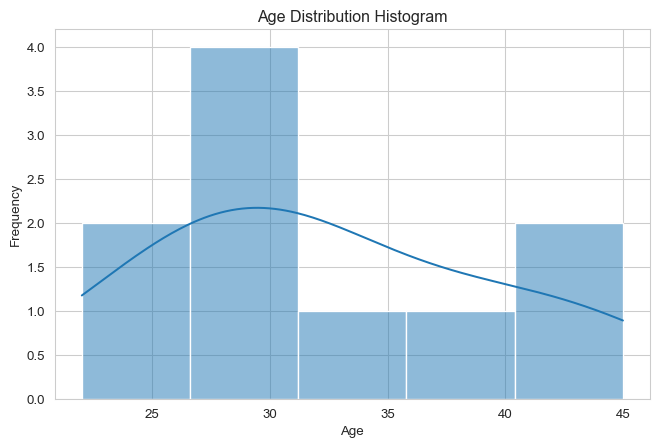
\includegraphics[keepaspectratio]{02-data-handling-exploration_files/figure-latex/cell-40-output-1.png}}

\pandocbounded{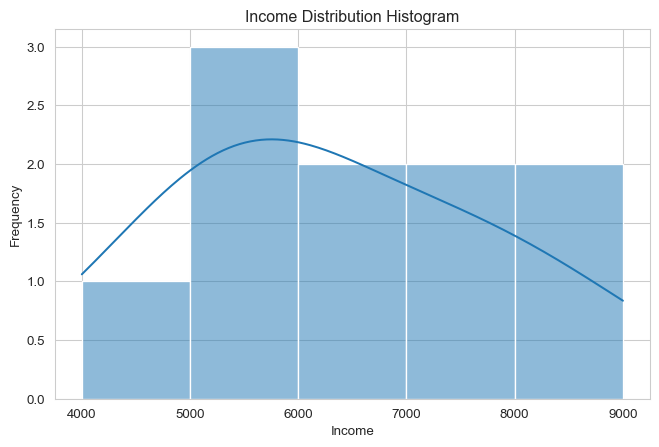
\includegraphics[keepaspectratio]{02-data-handling-exploration_files/figure-latex/cell-40-output-2.png}}

\begin{verbatim}
* **해석:** 히스토그램을 통해 데이터가 어떤 값 범위에 집중되어 있는지, 분포가 대칭적인지, 치우쳐 있는지(왜도) 등을 시각적으로 확인할 수 있습니다. `bins` 개수에 따라 모양이 달라질 수 있으므로 적절한 값 설정이 중요합니다.
\end{verbatim}

\begin{itemize}
\tightlist
\item
  \textbf{커널 밀도 추정 플롯 (Kernel Density Estimate Plot, KDE Plot):}

  \begin{itemize}
  \tightlist
  \item
    히스토그램을 부드러운 곡선 형태로 나타낸 것으로, 변수의 확률 밀도
    함수(Probability Density Function)를 추정하여 시각화합니다.
  \item
    Seaborn의 \texttt{kdeplot()} 또는
    \texttt{displot(kind=\textquotesingle{}kde\textquotesingle{})}
    함수를 사용합니다.
  \end{itemize}
\end{itemize}

\begin{Shaded}
\begin{Highlighting}[]
\CommentTok{\# Age 변수의 KDE 플롯}
\NormalTok{plt.figure(figsize}\OperatorTok{=}\NormalTok{(}\DecValTok{8}\NormalTok{, }\DecValTok{5}\NormalTok{))}
\NormalTok{sns.kdeplot(data}\OperatorTok{=}\NormalTok{df\_survey, x}\OperatorTok{=}\StringTok{\textquotesingle{}Age\textquotesingle{}}\NormalTok{, fill}\OperatorTok{=}\VariableTok{True}\NormalTok{) }\CommentTok{\# fill=True는 곡선 아래 영역 채우기}
\NormalTok{plt.title(}\StringTok{\textquotesingle{}Age Distribution KDE Plot\textquotesingle{}}\NormalTok{)}
\NormalTok{plt.xlabel(}\StringTok{\textquotesingle{}Age\textquotesingle{}}\NormalTok{)}
\NormalTok{plt.ylabel(}\StringTok{\textquotesingle{}Density\textquotesingle{}}\NormalTok{)}
\NormalTok{plt.show()}
\end{Highlighting}
\end{Shaded}

\pandocbounded{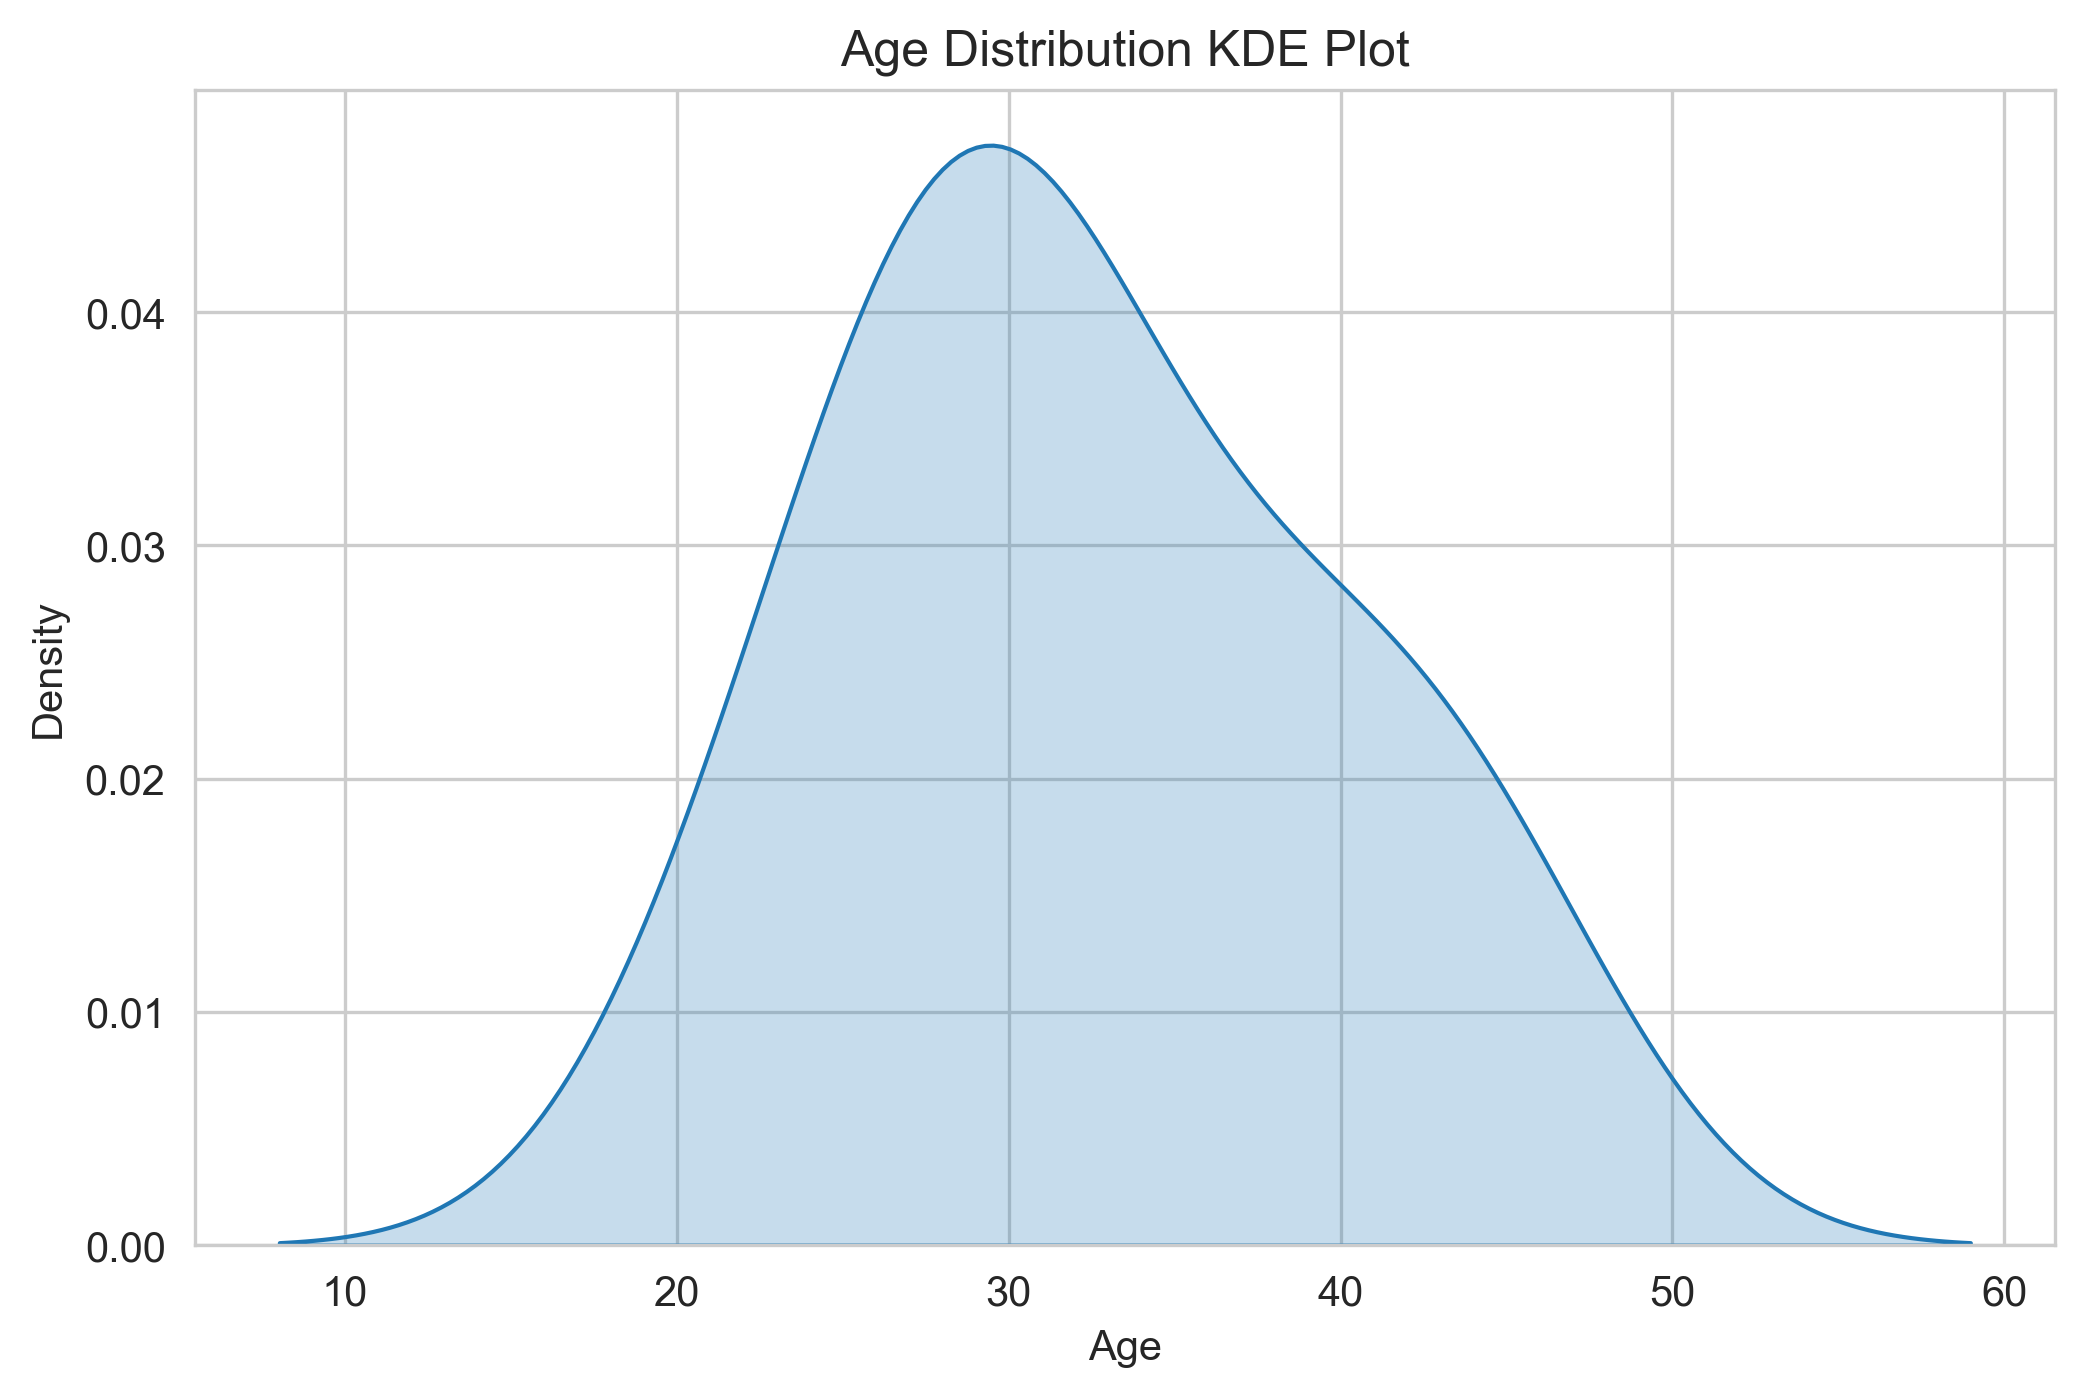
\includegraphics[keepaspectratio]{02-data-handling-exploration_files/figure-latex/cell-41-output-1.png}}

\begin{verbatim}
* **해석:** KDE 플롯은 히스토그램보다 분포의 형태를 더 매끄럽게 보여주지만, `bins` 설정이 없는 대신 대역폭(bandwidth) 파라미터에 따라 곡선의 평활도(smoothness)가 달라질 수 있습니다.
\end{verbatim}

\begin{itemize}
\tightlist
\item
  \textbf{박스 플롯 (Box Plot):}

  \begin{itemize}
  \tightlist
  \item
    데이터의 사분위수(Q1, Q2/중앙값, Q3), 최소/최대값(IQR 기준),
    이상치를 시각적으로 표현합니다. 데이터의 분포와 이상치 존재 여부를
    빠르게 파악하는 데 유용합니다 (2.2.2절, 2.3.2절 참고).
  \item
    Seaborn의 \texttt{boxplot()} 함수를 사용합니다.
  \end{itemize}
\end{itemize}

\begin{Shaded}
\begin{Highlighting}[]
\CommentTok{\# Income 변수의 박스 플롯}
\NormalTok{plt.figure(figsize}\OperatorTok{=}\NormalTok{(}\DecValTok{6}\NormalTok{, }\DecValTok{6}\NormalTok{))}
\NormalTok{sns.boxplot(data}\OperatorTok{=}\NormalTok{df\_survey, y}\OperatorTok{=}\StringTok{\textquotesingle{}Income\textquotesingle{}}\NormalTok{) }\CommentTok{\# y축에 변수 지정 시 세로 박스 플롯}
\NormalTok{plt.title(}\StringTok{\textquotesingle{}Income Distribution Box Plot\textquotesingle{}}\NormalTok{)}
\NormalTok{plt.ylabel(}\StringTok{\textquotesingle{}Income\textquotesingle{}}\NormalTok{)}
\NormalTok{plt.show()}

\CommentTok{\# SatisfactionScore 변수의 박스 플롯 (NaN 값은 자동으로 제외됨)}
\NormalTok{plt.figure(figsize}\OperatorTok{=}\NormalTok{(}\DecValTok{6}\NormalTok{, }\DecValTok{6}\NormalTok{))}
\NormalTok{sns.boxplot(data}\OperatorTok{=}\NormalTok{df\_survey, y}\OperatorTok{=}\StringTok{\textquotesingle{}SatisfactionScore\textquotesingle{}}\NormalTok{)}
\NormalTok{plt.title(}\StringTok{\textquotesingle{}Satisfaction Score Distribution Box Plot\textquotesingle{}}\NormalTok{)}
\NormalTok{plt.ylabel(}\StringTok{\textquotesingle{}Satisfaction Score\textquotesingle{}}\NormalTok{)}
\NormalTok{plt.show()}
\end{Highlighting}
\end{Shaded}

\pandocbounded{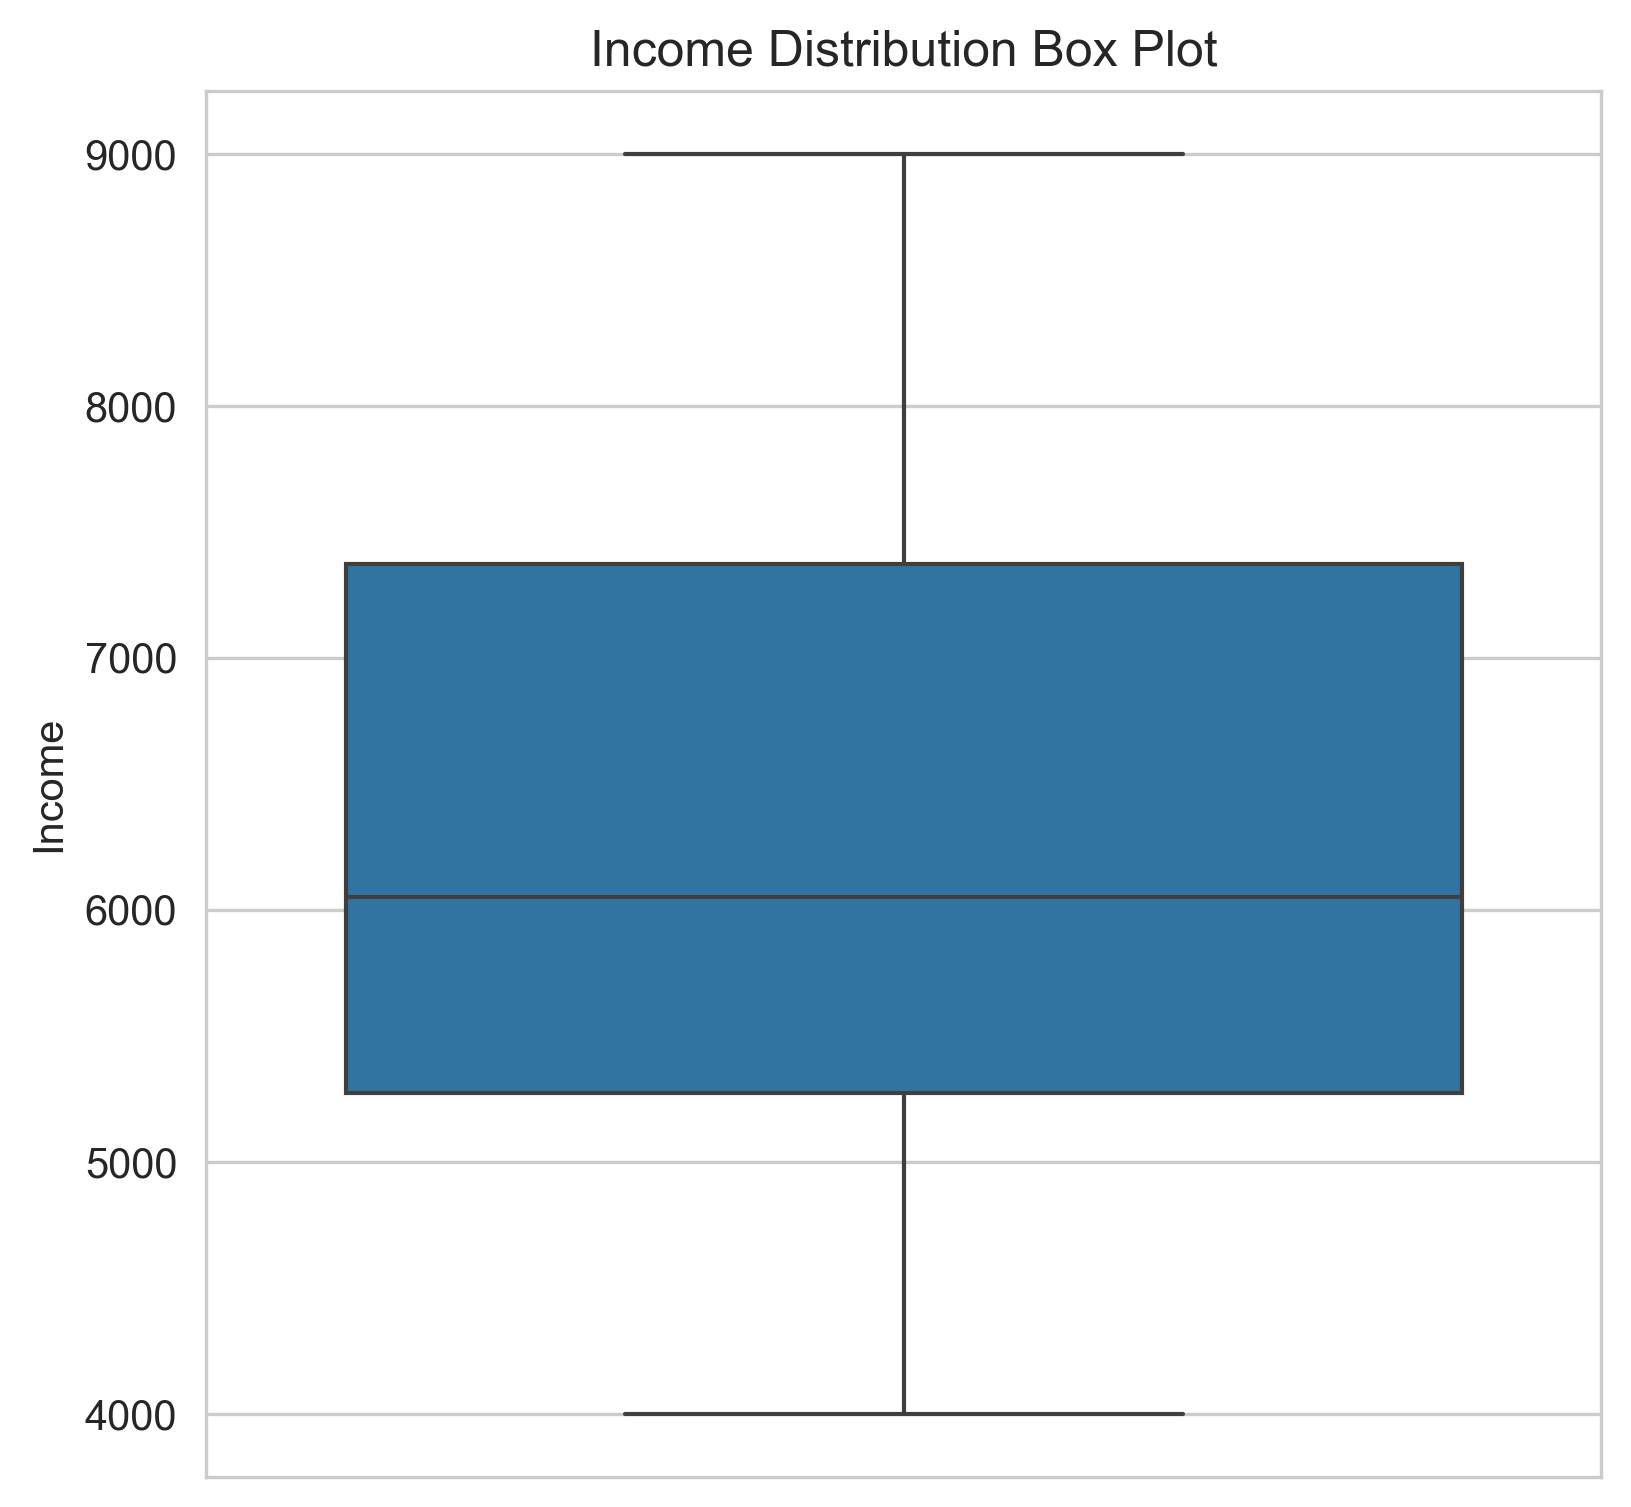
\includegraphics[keepaspectratio]{02-data-handling-exploration_files/figure-latex/cell-42-output-1.png}}

\pandocbounded{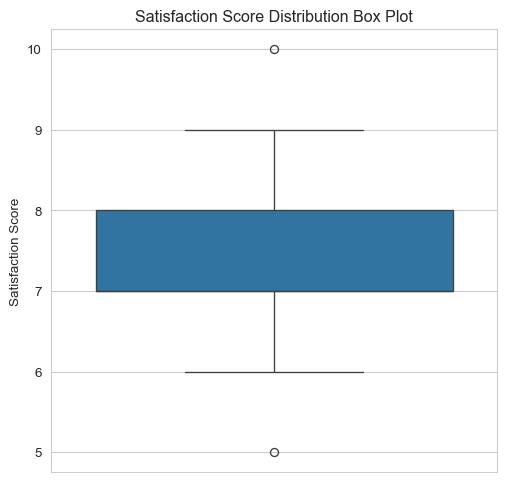
\includegraphics[keepaspectratio]{02-data-handling-exploration_files/figure-latex/cell-42-output-2.png}}

\begin{verbatim}
* **해석:** 상자의 하단/상단 선은 각각 Q1/Q3, 상자 안의 선은 중앙값(Q2)을 나타냅니다. 상자 길이는 IQR입니다. 상자 밖의 선(whisker)은 보통 IQR의 1.5배 범위 내의 데이터를 나타내며, 그 밖의 점들은 이상치(outlier)로 간주됩니다.
\end{verbatim}

\begin{itemize}
\tightlist
\item
  \textbf{카운트 플롯 (Count Plot):}

  \begin{itemize}
  \tightlist
  \item
    범주형 변수의 각 범주별 빈도를 막대 그래프로 시각화합니다.
  \item
    Seaborn의 \texttt{countplot()} 함수를 사용합니다.
  \end{itemize}
\end{itemize}

\begin{Shaded}
\begin{Highlighting}[]
\CommentTok{\# Gender 변수의 카운트 플롯}
\NormalTok{plt.figure(figsize}\OperatorTok{=}\NormalTok{(}\DecValTok{6}\NormalTok{, }\DecValTok{5}\NormalTok{))}
\NormalTok{sns.countplot(data}\OperatorTok{=}\NormalTok{df\_survey, x}\OperatorTok{=}\StringTok{\textquotesingle{}Gender\textquotesingle{}}\NormalTok{, palette}\OperatorTok{=}\StringTok{\textquotesingle{}viridis\textquotesingle{}}\NormalTok{) }\CommentTok{\# palette로 색상 지정}
\NormalTok{plt.title(}\StringTok{\textquotesingle{}Gender Count Plot\textquotesingle{}}\NormalTok{)}
\NormalTok{plt.xlabel(}\StringTok{\textquotesingle{}Gender\textquotesingle{}}\NormalTok{)}
\NormalTok{plt.ylabel(}\StringTok{\textquotesingle{}Count\textquotesingle{}}\NormalTok{)}
\NormalTok{plt.show()}

\CommentTok{\# EducationLevel 변수의 카운트 플롯}
\NormalTok{plt.figure(figsize}\OperatorTok{=}\NormalTok{(}\DecValTok{8}\NormalTok{, }\DecValTok{5}\NormalTok{))}
\NormalTok{sns.countplot(data}\OperatorTok{=}\NormalTok{df\_survey, y}\OperatorTok{=}\StringTok{\textquotesingle{}EducationLevel\textquotesingle{}}\NormalTok{, order}\OperatorTok{=}\NormalTok{df\_survey[}\StringTok{\textquotesingle{}EducationLevel\textquotesingle{}}\NormalTok{].value\_counts().index) }\CommentTok{\# 빈도순 정렬}
\NormalTok{plt.title(}\StringTok{\textquotesingle{}Education Level Count Plot\textquotesingle{}}\NormalTok{)}
\NormalTok{plt.xlabel(}\StringTok{\textquotesingle{}Count\textquotesingle{}}\NormalTok{)}
\NormalTok{plt.ylabel(}\StringTok{\textquotesingle{}Education Level\textquotesingle{}}\NormalTok{)}
\NormalTok{plt.tight\_layout() }\CommentTok{\# 레이블 잘림 방지}
\NormalTok{plt.show()}
\end{Highlighting}
\end{Shaded}

\begin{verbatim}
C:\Users\voidm\AppData\Local\Temp\ipykernel_34588\3407003983.py:3: FutureWarning:



Passing `palette` without assigning `hue` is deprecated and will be removed in v0.14.0. Assign the `x` variable to `hue` and set `legend=False` for the same effect.

\end{verbatim}

\pandocbounded{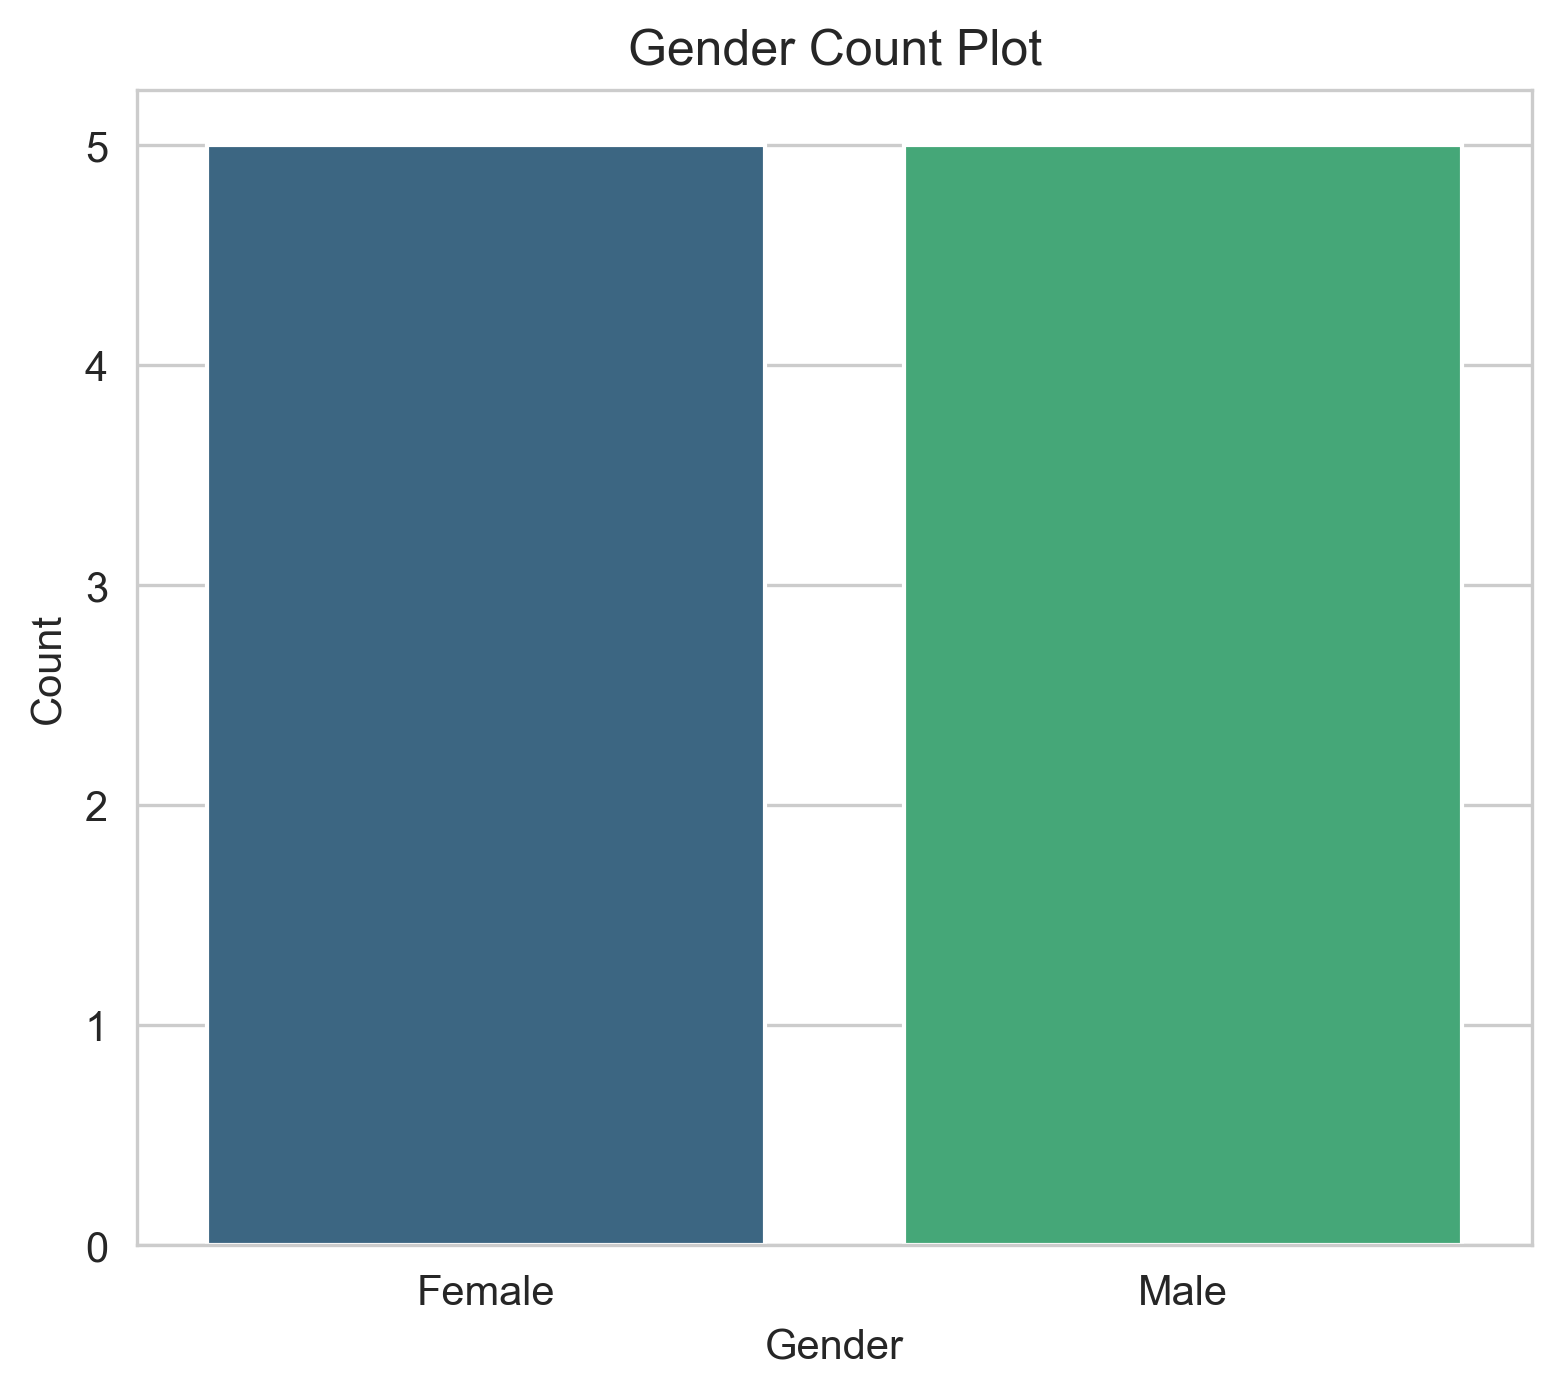
\includegraphics[keepaspectratio]{02-data-handling-exploration_files/figure-latex/cell-43-output-2.png}}

\pandocbounded{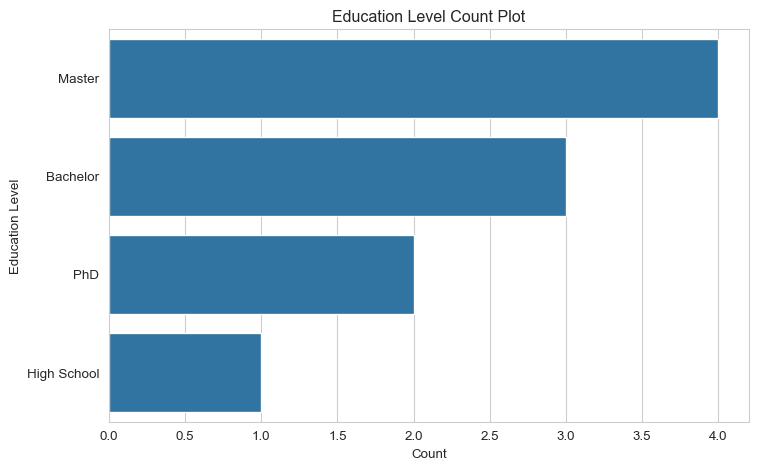
\includegraphics[keepaspectratio]{02-data-handling-exploration_files/figure-latex/cell-43-output-3.png}}

\begin{verbatim}
* **해석:** 각 막대의 길이는 해당 범주의 빈도를 나타냅니다. 범주별 상대적인 크기를 쉽게 비교할 수 있습니다.
\end{verbatim}

\subsection{2.4.2 이변량 시각화 (Bivariate
Visualization)}\label{uxc774uxbcc0uxb7c9-uxc2dcuxac01uxd654-bivariate-visualization}

이변량 시각화는 두 변수 간의 관계를 탐색하는 데 사용됩니다. 변수의
종류(연속형/범주형)에 따라 적합한 그래프 유형이 다릅니다.

\begin{itemize}
\tightlist
\item
  \textbf{산점도 (Scatter Plot):}

  \begin{itemize}
  \tightlist
  \item
    두 연속형 변수 간의 관계를 시각화하는 데 가장 널리 사용됩니다. 각
    데이터 포인트를 2차원 평면 위에 점으로 나타냅니다.
  \item
    변수 간 선형 관계, 비선형 관계, 군집, 이상치 등을 파악할 수
    있습니다.
  \item
    Seaborn의 \texttt{scatterplot()} 또는
    \texttt{relplot(kind=\textquotesingle{}scatter\textquotesingle{})}
    함수를 사용합니다.
  \end{itemize}
\end{itemize}

\begin{Shaded}
\begin{Highlighting}[]
\CommentTok{\# Age와 Income 간의 산점도}
\NormalTok{plt.figure(figsize}\OperatorTok{=}\NormalTok{(}\DecValTok{8}\NormalTok{, }\DecValTok{6}\NormalTok{))}
\NormalTok{sns.scatterplot(data}\OperatorTok{=}\NormalTok{df\_survey, x}\OperatorTok{=}\StringTok{\textquotesingle{}Age\textquotesingle{}}\NormalTok{, y}\OperatorTok{=}\StringTok{\textquotesingle{}Income\textquotesingle{}}\NormalTok{, hue}\OperatorTok{=}\StringTok{\textquotesingle{}Gender\textquotesingle{}}\NormalTok{, style}\OperatorTok{=}\StringTok{\textquotesingle{}EducationLevel\textquotesingle{}}\NormalTok{, s}\OperatorTok{=}\DecValTok{100}\NormalTok{) }\CommentTok{\# hue/style/size로 추가 변수 표현 가능}
\NormalTok{plt.title(}\StringTok{\textquotesingle{}Scatter Plot of Age vs Income\textquotesingle{}}\NormalTok{)}
\NormalTok{plt.xlabel(}\StringTok{\textquotesingle{}Age\textquotesingle{}}\NormalTok{)}
\NormalTok{plt.ylabel(}\StringTok{\textquotesingle{}Income\textquotesingle{}}\NormalTok{)}
\NormalTok{plt.legend(bbox\_to\_anchor}\OperatorTok{=}\NormalTok{(}\FloatTok{1.05}\NormalTok{, }\DecValTok{1}\NormalTok{), loc}\OperatorTok{=}\StringTok{\textquotesingle{}upper left\textquotesingle{}}\NormalTok{) }\CommentTok{\# 범례 위치 조정}
\NormalTok{plt.tight\_layout()}
\NormalTok{plt.show()}
\end{Highlighting}
\end{Shaded}

\pandocbounded{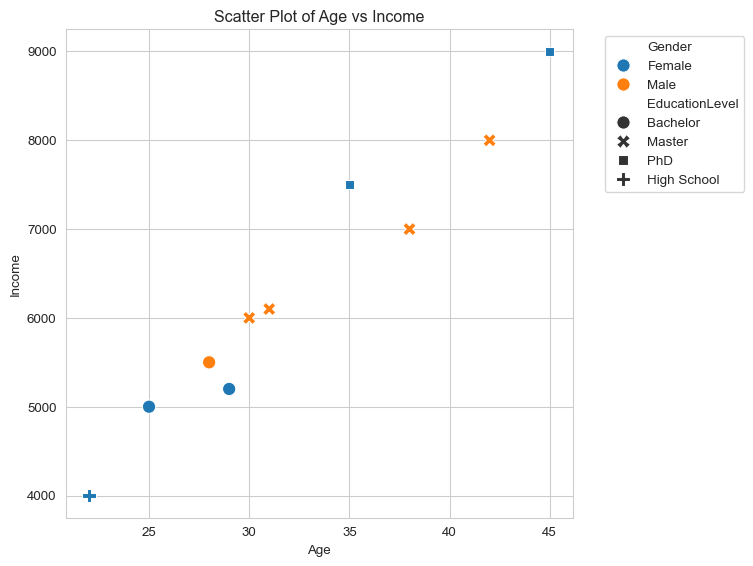
\includegraphics[keepaspectratio]{02-data-handling-exploration_files/figure-latex/cell-44-output-1.png}}

\begin{verbatim}
* **해석:** 점들의 분포 패턴을 통해 두 변수 간의 관계 방향(양의 관계, 음의 관계)과 강도를 추측할 수 있습니다. `hue`, `style`, `size` 등의 옵션을 활용하면 추가적인 범주형 또는 연속형 변수의 정보를 함께 표현할 수 있습니다 (다변량 시각화의 기초).
\end{verbatim}

\begin{itemize}
\tightlist
\item
  \textbf{라인 플롯 (Line Plot):}

  \begin{itemize}
  \tightlist
  \item
    주로 시간의 흐름에 따른 연속형 변수의 변화 추세를 시각화하는 데
    사용됩니다. (현재 \texttt{df\_survey} 데이터는 시계열이 아니므로
    예시는 생략하지만, 개념 설명)
  \item
    x축이 순서(시간, 단계 등)를 나타내는 경우 유용합니다.
  \item
    Seaborn의 \texttt{lineplot()} 또는
    \texttt{relplot(kind=\textquotesingle{}line\textquotesingle{})}
    함수를 사용합니다.
  \item
    \textbf{사용 예시:} 연도별 평균 소득 변화, 실험 단계별 반응 시간
    변화 등.
  \end{itemize}
\item
  \textbf{비교 박스 플롯 / 바이올린 플롯 (Box Plot / Violin Plot for
  Comparison):}

  \begin{itemize}
  \tightlist
  \item
    범주형 변수의 각 범주에 따른 연속형 변수의 분포를 비교할 때
    유용합니다.
  \item
    \textbf{박스 플롯:} 여러 그룹의 분포를 사분위수 기준으로 간결하게
    비교합니다.
  \item
    \textbf{바이올린 플롯:} 박스 플롯에 KDE(커널 밀도 추정)를 결합하여
    분포의 형태까지 함께 보여줍니다.
  \item
    Seaborn의 \texttt{boxplot()}, \texttt{violinplot()} 함수를
    사용합니다.
  \end{itemize}
\end{itemize}

\begin{Shaded}
\begin{Highlighting}[]
\CommentTok{\# EducationLevel 별 Income 분포 비교 (박스 플롯)}
\NormalTok{plt.figure(figsize}\OperatorTok{=}\NormalTok{(}\DecValTok{10}\NormalTok{, }\DecValTok{6}\NormalTok{))}
\NormalTok{sns.boxplot(data}\OperatorTok{=}\NormalTok{df\_survey, x}\OperatorTok{=}\StringTok{\textquotesingle{}EducationLevel\textquotesingle{}}\NormalTok{, y}\OperatorTok{=}\StringTok{\textquotesingle{}Income\textquotesingle{}}\NormalTok{, order}\OperatorTok{=}\NormalTok{[}\StringTok{\textquotesingle{}High School\textquotesingle{}}\NormalTok{, }\StringTok{\textquotesingle{}Bachelor\textquotesingle{}}\NormalTok{, }\StringTok{\textquotesingle{}Master\textquotesingle{}}\NormalTok{, }\StringTok{\textquotesingle{}PhD\textquotesingle{}}\NormalTok{]) }\CommentTok{\# 순서 지정}
\NormalTok{plt.title(}\StringTok{\textquotesingle{}Income Distribution by Education Level (Box Plot)\textquotesingle{}}\NormalTok{)}
\NormalTok{plt.xlabel(}\StringTok{\textquotesingle{}Education Level\textquotesingle{}}\NormalTok{)}
\NormalTok{plt.ylabel(}\StringTok{\textquotesingle{}Income\textquotesingle{}}\NormalTok{)}
\NormalTok{plt.xticks(rotation}\OperatorTok{=}\DecValTok{15}\NormalTok{) }\CommentTok{\# x축 레이블 회전}
\NormalTok{plt.tight\_layout()}
\NormalTok{plt.show()}

\CommentTok{\# Gender 별 SatisfactionScore 분포 비교 (바이올린 플롯)}
\NormalTok{plt.figure(figsize}\OperatorTok{=}\NormalTok{(}\DecValTok{8}\NormalTok{, }\DecValTok{6}\NormalTok{))}
\NormalTok{sns.violinplot(data}\OperatorTok{=}\NormalTok{df\_survey.dropna(subset}\OperatorTok{=}\NormalTok{[}\StringTok{\textquotesingle{}SatisfactionScore\textquotesingle{}}\NormalTok{]), x}\OperatorTok{=}\StringTok{\textquotesingle{}Gender\textquotesingle{}}\NormalTok{, y}\OperatorTok{=}\StringTok{\textquotesingle{}SatisfactionScore\textquotesingle{}}\NormalTok{, inner}\OperatorTok{=}\StringTok{\textquotesingle{}quartile\textquotesingle{}}\NormalTok{) }\CommentTok{\# inner=\textquotesingle{}quartile\textquotesingle{}은 사분위수 표시}
\NormalTok{plt.title(}\StringTok{\textquotesingle{}Satisfaction Score Distribution by Gender (Violin Plot)\textquotesingle{}}\NormalTok{)}
\NormalTok{plt.xlabel(}\StringTok{\textquotesingle{}Gender\textquotesingle{}}\NormalTok{)}
\NormalTok{plt.ylabel(}\StringTok{\textquotesingle{}Satisfaction Score\textquotesingle{}}\NormalTok{)}
\NormalTok{plt.show()}
\end{Highlighting}
\end{Shaded}

\pandocbounded{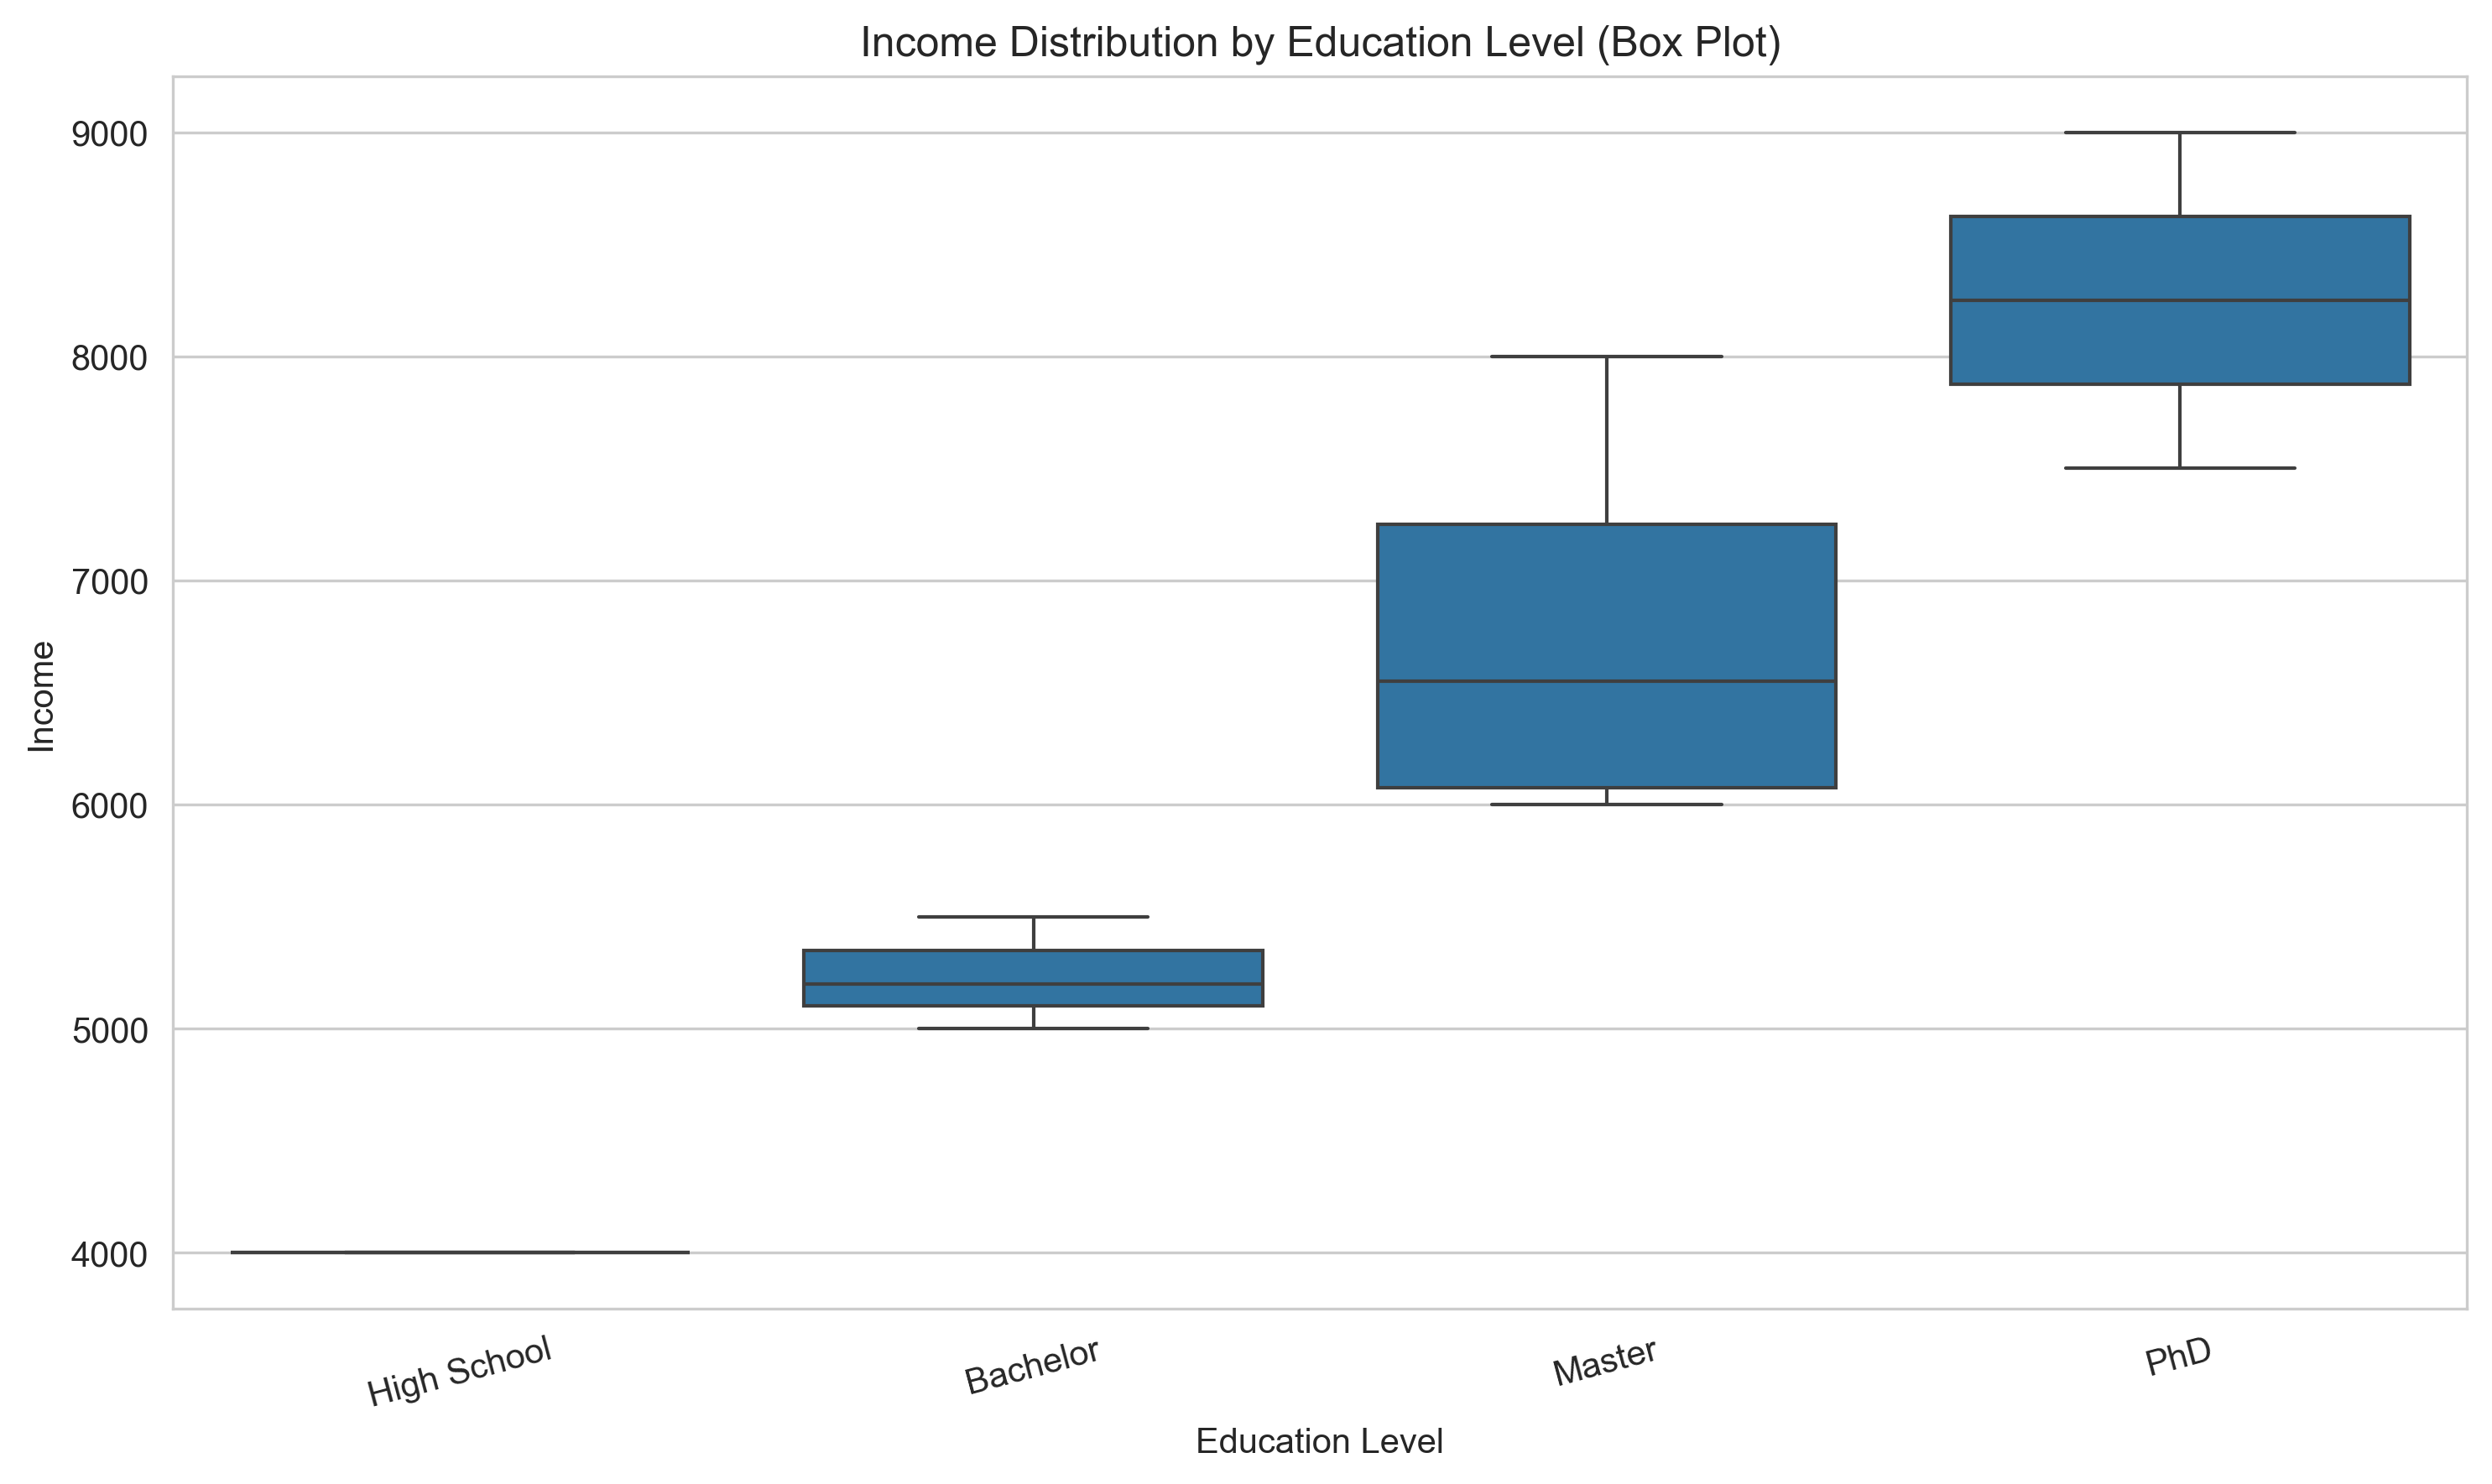
\includegraphics[keepaspectratio]{02-data-handling-exploration_files/figure-latex/cell-45-output-1.png}}

\pandocbounded{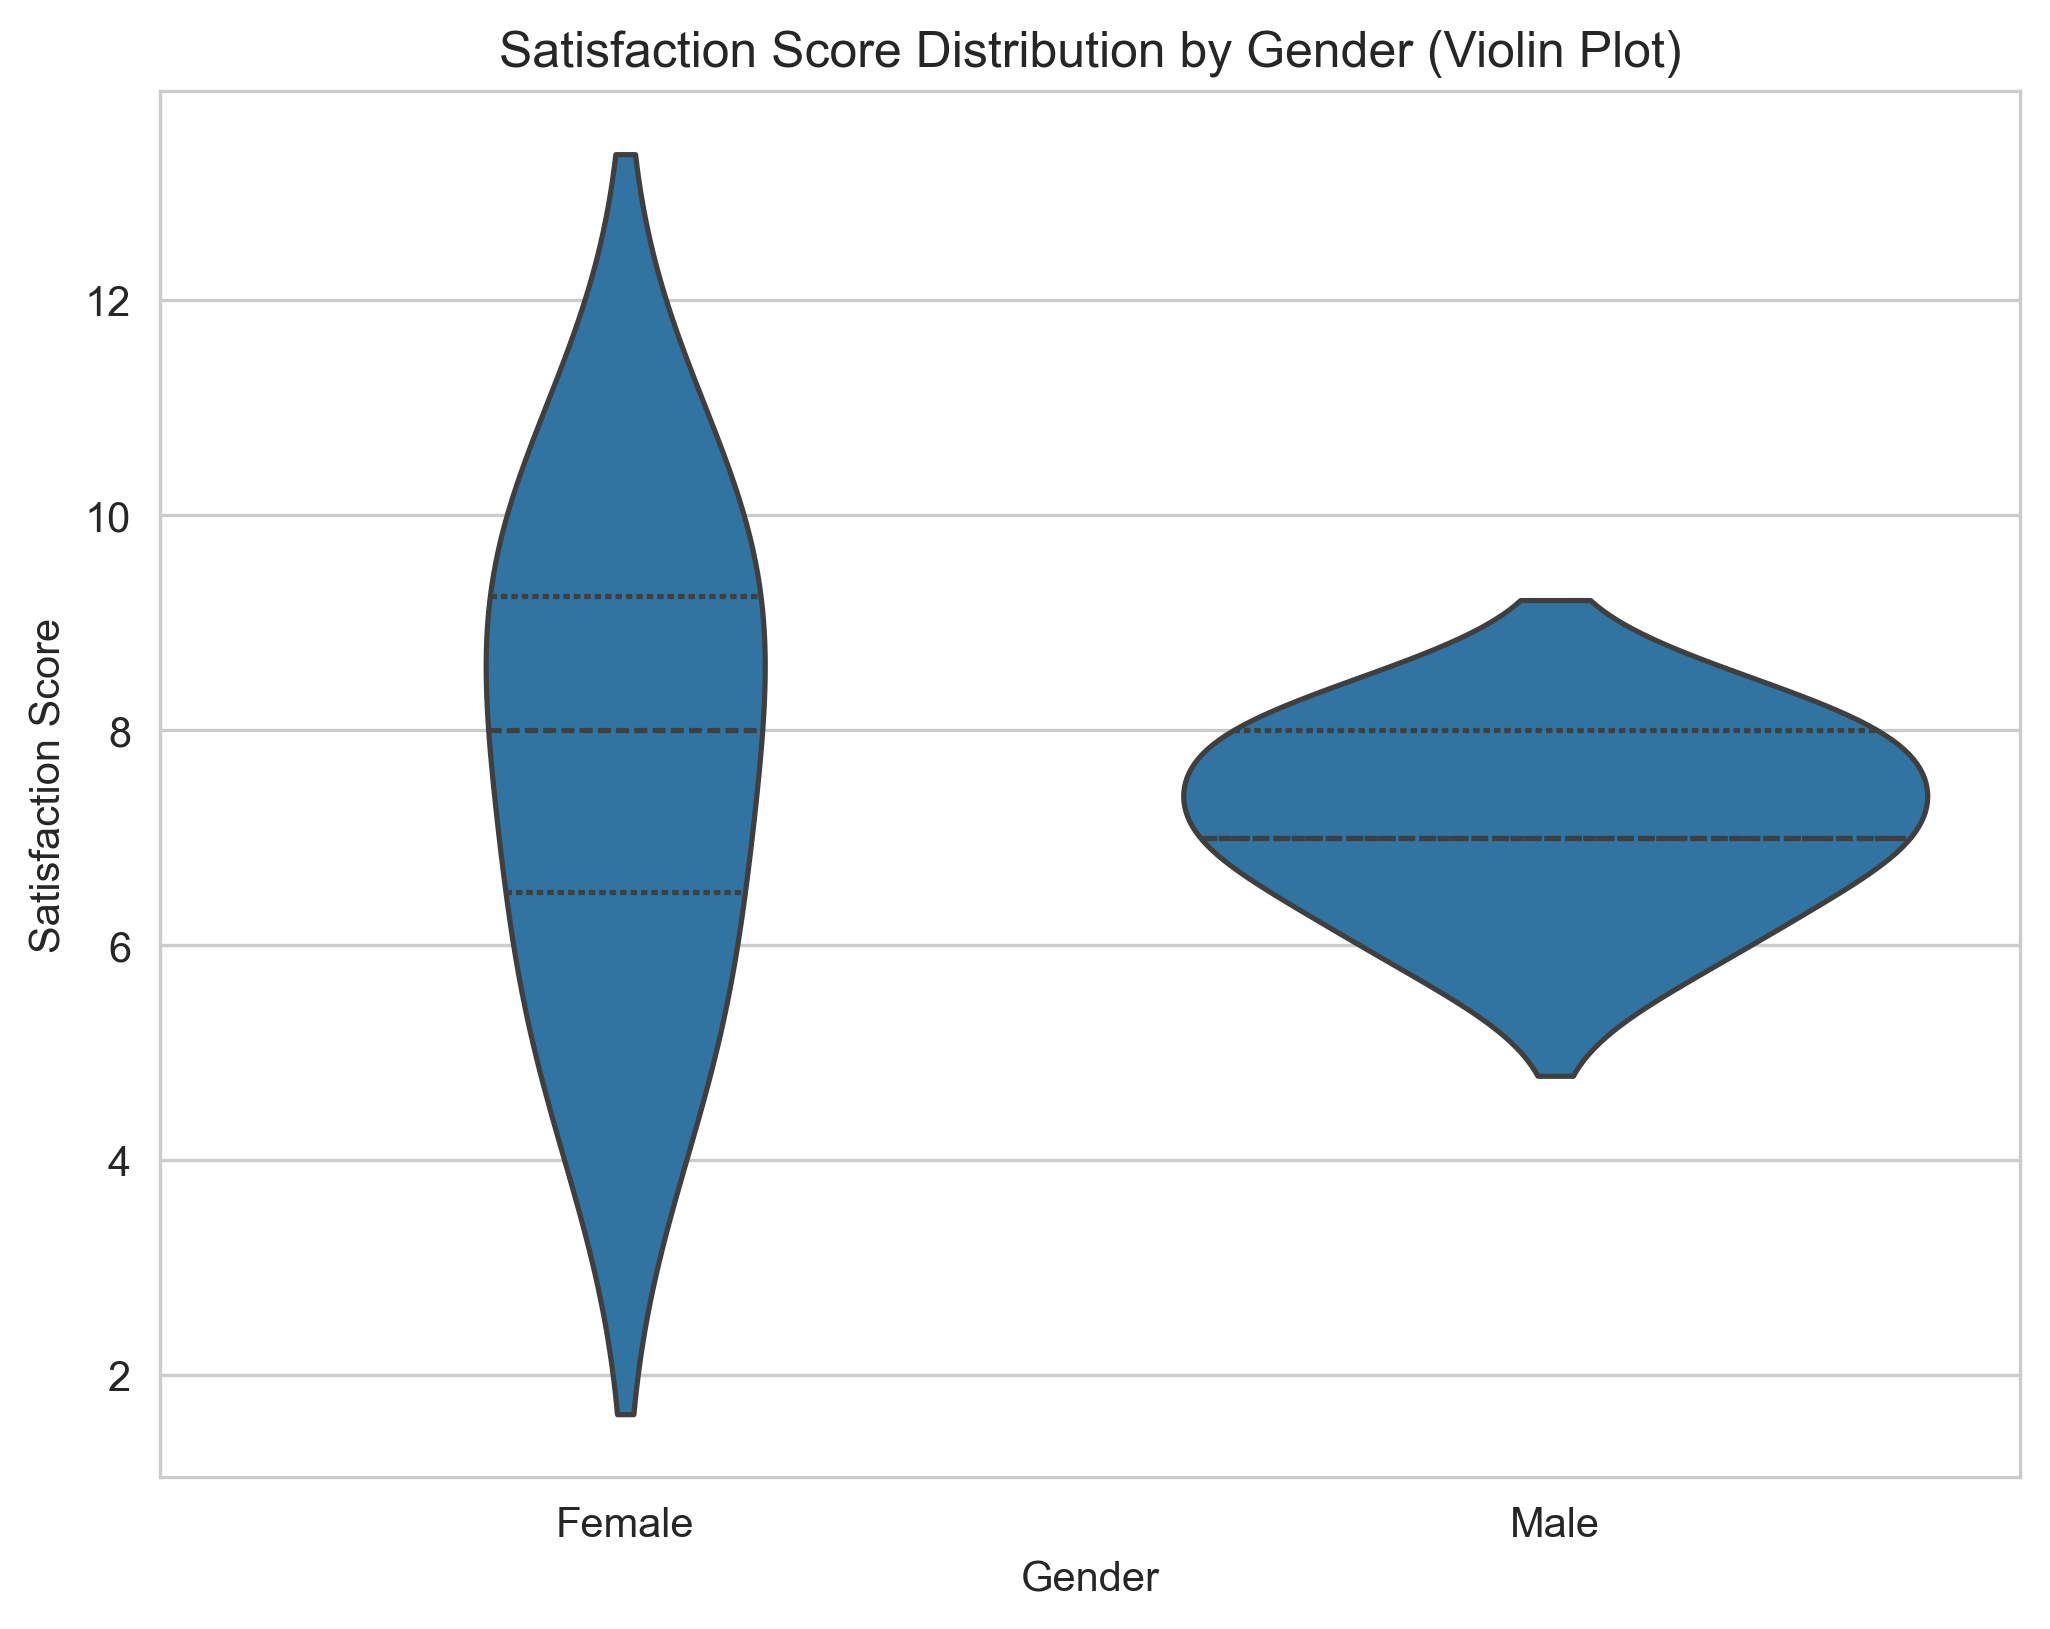
\includegraphics[keepaspectratio]{02-data-handling-exploration_files/figure-latex/cell-45-output-2.png}}

\begin{verbatim}
* **해석:** 그룹 간 중심 경향성(중앙값), 퍼짐 정도(IQR, 바이올린의 폭), 이상치 유무 등을 비교하여 집단 간 차이를 시각적으로 탐색할 수 있습니다.
\end{verbatim}

\begin{itemize}
\tightlist
\item
  \textbf{비교 막대 플롯 (Bar Plot for Comparison):}

  \begin{itemize}
  \tightlist
  \item
    범주형 변수의 각 범주에 따른 연속형 변수의 \textbf{대표값(기본값:
    평균)}을 막대로 비교하여 시각화합니다. 막대 위의 선(오차 막대)은
    보통 신뢰 구간(Confidence Interval)을 나타냅니다.
  \item
    Seaborn의 \texttt{barplot()} 함수를 사용합니다. \texttt{estimator}
    인자를 통해 평균 외 다른 통계량(중앙값 등)을 지정할 수 있습니다.
  \end{itemize}
\end{itemize}

\begin{Shaded}
\begin{Highlighting}[]
\CommentTok{\# EducationLevel 별 평균 Income 비교 (막대 플롯)}
\NormalTok{plt.figure(figsize}\OperatorTok{=}\NormalTok{(}\DecValTok{10}\NormalTok{, }\DecValTok{6}\NormalTok{))}
\CommentTok{\# np.mean 대신 다른 estimator 사용 가능 (예: estimator=np.median)}
\NormalTok{sns.barplot(data}\OperatorTok{=}\NormalTok{df\_survey, x}\OperatorTok{=}\StringTok{\textquotesingle{}EducationLevel\textquotesingle{}}\NormalTok{, y}\OperatorTok{=}\StringTok{\textquotesingle{}Income\textquotesingle{}}\NormalTok{, order}\OperatorTok{=}\NormalTok{[}\StringTok{\textquotesingle{}High School\textquotesingle{}}\NormalTok{, }\StringTok{\textquotesingle{}Bachelor\textquotesingle{}}\NormalTok{, }\StringTok{\textquotesingle{}Master\textquotesingle{}}\NormalTok{, }\StringTok{\textquotesingle{}PhD\textquotesingle{}}\NormalTok{], ci}\OperatorTok{=}\StringTok{\textquotesingle{}sd\textquotesingle{}}\NormalTok{) }\CommentTok{\# ci=\textquotesingle{}sd\textquotesingle{}는 표준편차 표시}
\NormalTok{plt.title(}\StringTok{\textquotesingle{}Average Income by Education Level (Bar Plot)\textquotesingle{}}\NormalTok{)}
\NormalTok{plt.xlabel(}\StringTok{\textquotesingle{}Education Level\textquotesingle{}}\NormalTok{)}
\NormalTok{plt.ylabel(}\StringTok{\textquotesingle{}Average Income\textquotesingle{}}\NormalTok{)}
\NormalTok{plt.xticks(rotation}\OperatorTok{=}\DecValTok{15}\NormalTok{)}
\NormalTok{plt.tight\_layout()}
\NormalTok{plt.show()}
\end{Highlighting}
\end{Shaded}

\begin{verbatim}
C:\Users\voidm\AppData\Local\Temp\ipykernel_34588\1340021530.py:4: FutureWarning:



The `ci` parameter is deprecated. Use `errorbar='sd'` for the same effect.

\end{verbatim}

\pandocbounded{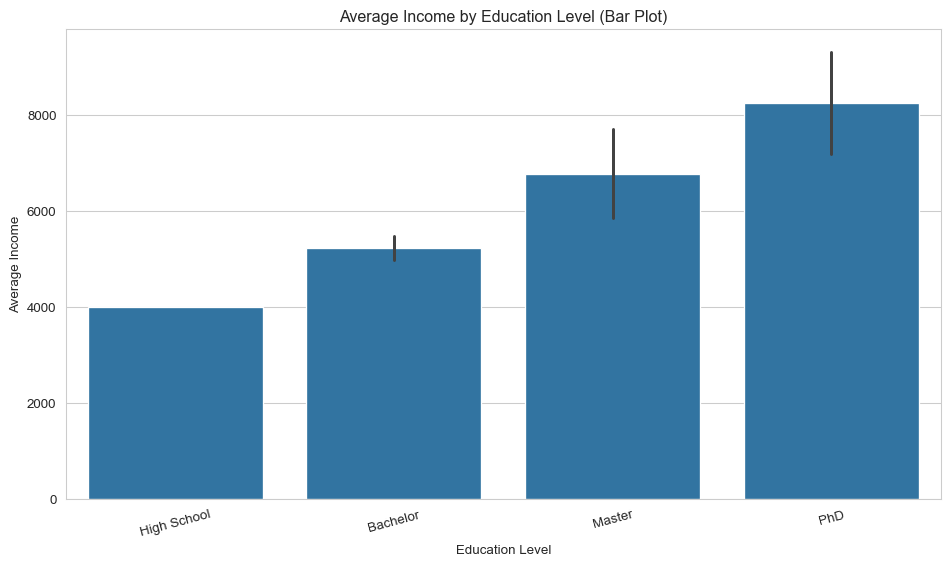
\includegraphics[keepaspectratio]{02-data-handling-exploration_files/figure-latex/cell-46-output-2.png}}

\begin{verbatim}
* **해석:** 그룹 간 평균값의 차이를 직관적으로 비교할 수 있습니다. 오차 막대를 통해 값의 불확실성(분산 정도)도 함께 고려해야 합니다. (`countplot`은 단순히 빈도를 세는 반면, `barplot`은 y축 변수의 통계량을 계산하여 보여준다는 차이가 있습니다.)
\end{verbatim}

\subsection{2.4.3 다변수 시각화 간략 소개 (Brief Introduction to
Multivariate
Visualization)}\label{uxb2e4uxbcc0uxc218-uxc2dcuxac01uxd654-uxac04uxb7b5-uxc18cuxac1c-brief-introduction-to-multivariate-visualization}

세 개 이상의 변수 간 관계를 동시에 탐색하기 위한 시각화 기법입니다.

\begin{itemize}
\tightlist
\item
  \textbf{Pair Plot:}

  \begin{itemize}
  \tightlist
  \item
    데이터프레임 내 여러 수치형 변수들 간의 모든 쌍(pair)에 대한
    산점도를 그리고, 대각선에는 각 변수의 분포(히스토그램 또는 KDE)를
    보여줍니다. 변수 간 관계를 전반적으로 빠르게 파악하는 데 매우
    유용합니다.
  \item
    Seaborn의 \texttt{pairplot()} 함수를 사용합니다.
  \end{itemize}
\end{itemize}

\begin{Shaded}
\begin{Highlighting}[]
\CommentTok{\# Age, SatisfactionScore, Income 변수 간 Pair Plot}
\CommentTok{\# 결측치가 있으면 오류 발생 가능하므로 제거하거나 처리 후 사용}
\NormalTok{sns.pairplot(df\_survey.dropna(subset}\OperatorTok{=}\NormalTok{[}\StringTok{\textquotesingle{}SatisfactionScore\textquotesingle{}}\NormalTok{])[[}\StringTok{\textquotesingle{}Age\textquotesingle{}}\NormalTok{, }\StringTok{\textquotesingle{}SatisfactionScore\textquotesingle{}}\NormalTok{, }\StringTok{\textquotesingle{}Income\textquotesingle{}}\NormalTok{]], diag\_kind}\OperatorTok{=}\StringTok{\textquotesingle{}kde\textquotesingle{}}\NormalTok{, corner}\OperatorTok{=}\VariableTok{True}\NormalTok{) }\CommentTok{\# corner=True는 중복되는 위쪽 삼각형 제외}
\NormalTok{plt.suptitle(}\StringTok{\textquotesingle{}Pair Plot of Key Numerical Variables\textquotesingle{}}\NormalTok{, y}\OperatorTok{=}\FloatTok{1.02}\NormalTok{) }\CommentTok{\# 전체 제목 추가}
\NormalTok{plt.show()}
\end{Highlighting}
\end{Shaded}

\pandocbounded{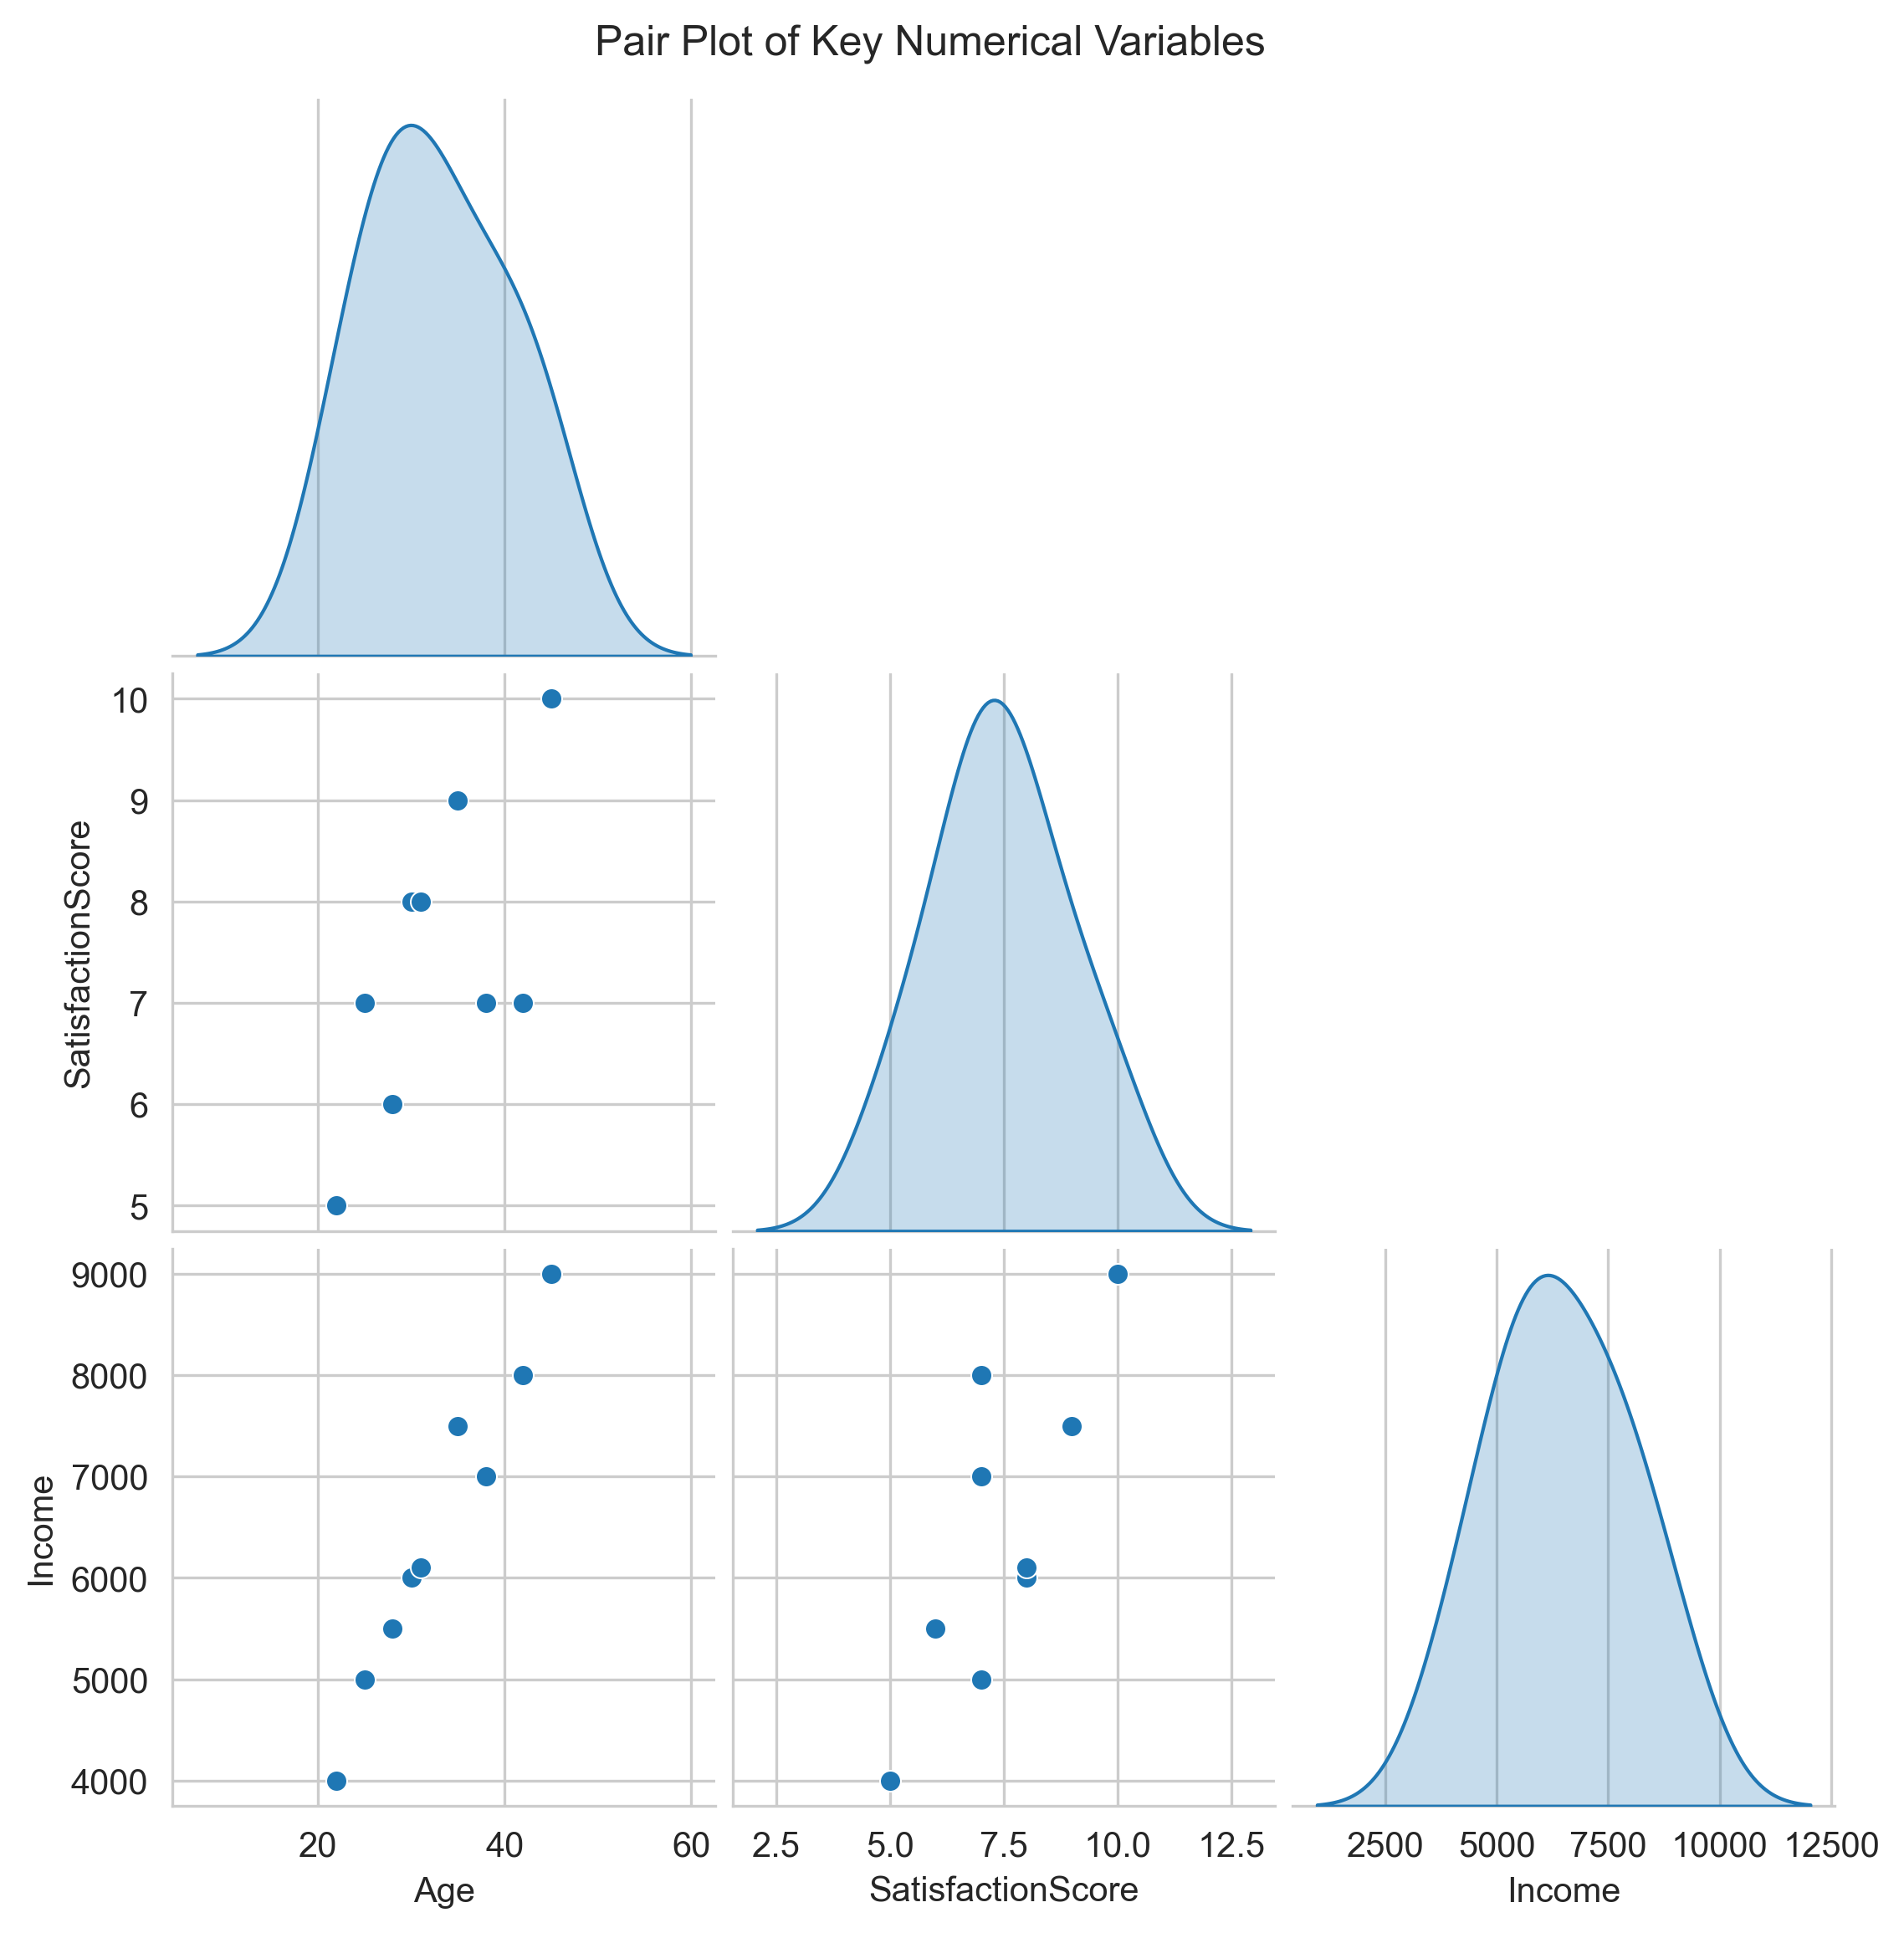
\includegraphics[keepaspectratio]{02-data-handling-exploration_files/figure-latex/cell-47-output-1.png}}

\begin{itemize}
\tightlist
\item
  \textbf{히트맵 (Heatmap):}

  \begin{itemize}
  \tightlist
  \item
    매트릭스 형태의 데이터를 색상을 이용하여 시각화합니다. 주로 변수 간
    상관계수 행렬(Correlation Matrix)을 시각화하는 데 많이 사용됩니다.
  \item
    Seaborn의 \texttt{heatmap()} 함수를 사용합니다.
  \end{itemize}
\end{itemize}

\begin{Shaded}
\begin{Highlighting}[]
\CommentTok{\# 수치형 변수 간 상관계수 계산}
\NormalTok{correlation\_matrix }\OperatorTok{=}\NormalTok{ df\_survey[[}\StringTok{\textquotesingle{}Age\textquotesingle{}}\NormalTok{, }\StringTok{\textquotesingle{}SatisfactionScore\textquotesingle{}}\NormalTok{, }\StringTok{\textquotesingle{}Income\textquotesingle{}}\NormalTok{]].corr()}

\CommentTok{\# 상관계수 행렬 히트맵 시각화}
\NormalTok{plt.figure(figsize}\OperatorTok{=}\NormalTok{(}\DecValTok{7}\NormalTok{, }\DecValTok{5}\NormalTok{))}
\NormalTok{sns.heatmap(correlation\_matrix, annot}\OperatorTok{=}\VariableTok{True}\NormalTok{, cmap}\OperatorTok{=}\StringTok{\textquotesingle{}coolwarm\textquotesingle{}}\NormalTok{, fmt}\OperatorTok{=}\StringTok{\textquotesingle{}.2f\textquotesingle{}}\NormalTok{, linewidths}\OperatorTok{=}\FloatTok{.5}\NormalTok{) }\CommentTok{\# annot=True는 값 표시, cmap은 색상 맵, fmt는 소수점 자리}
\NormalTok{plt.title(}\StringTok{\textquotesingle{}Correlation Matrix Heatmap\textquotesingle{}}\NormalTok{)}
\NormalTok{plt.show()}
\end{Highlighting}
\end{Shaded}

\pandocbounded{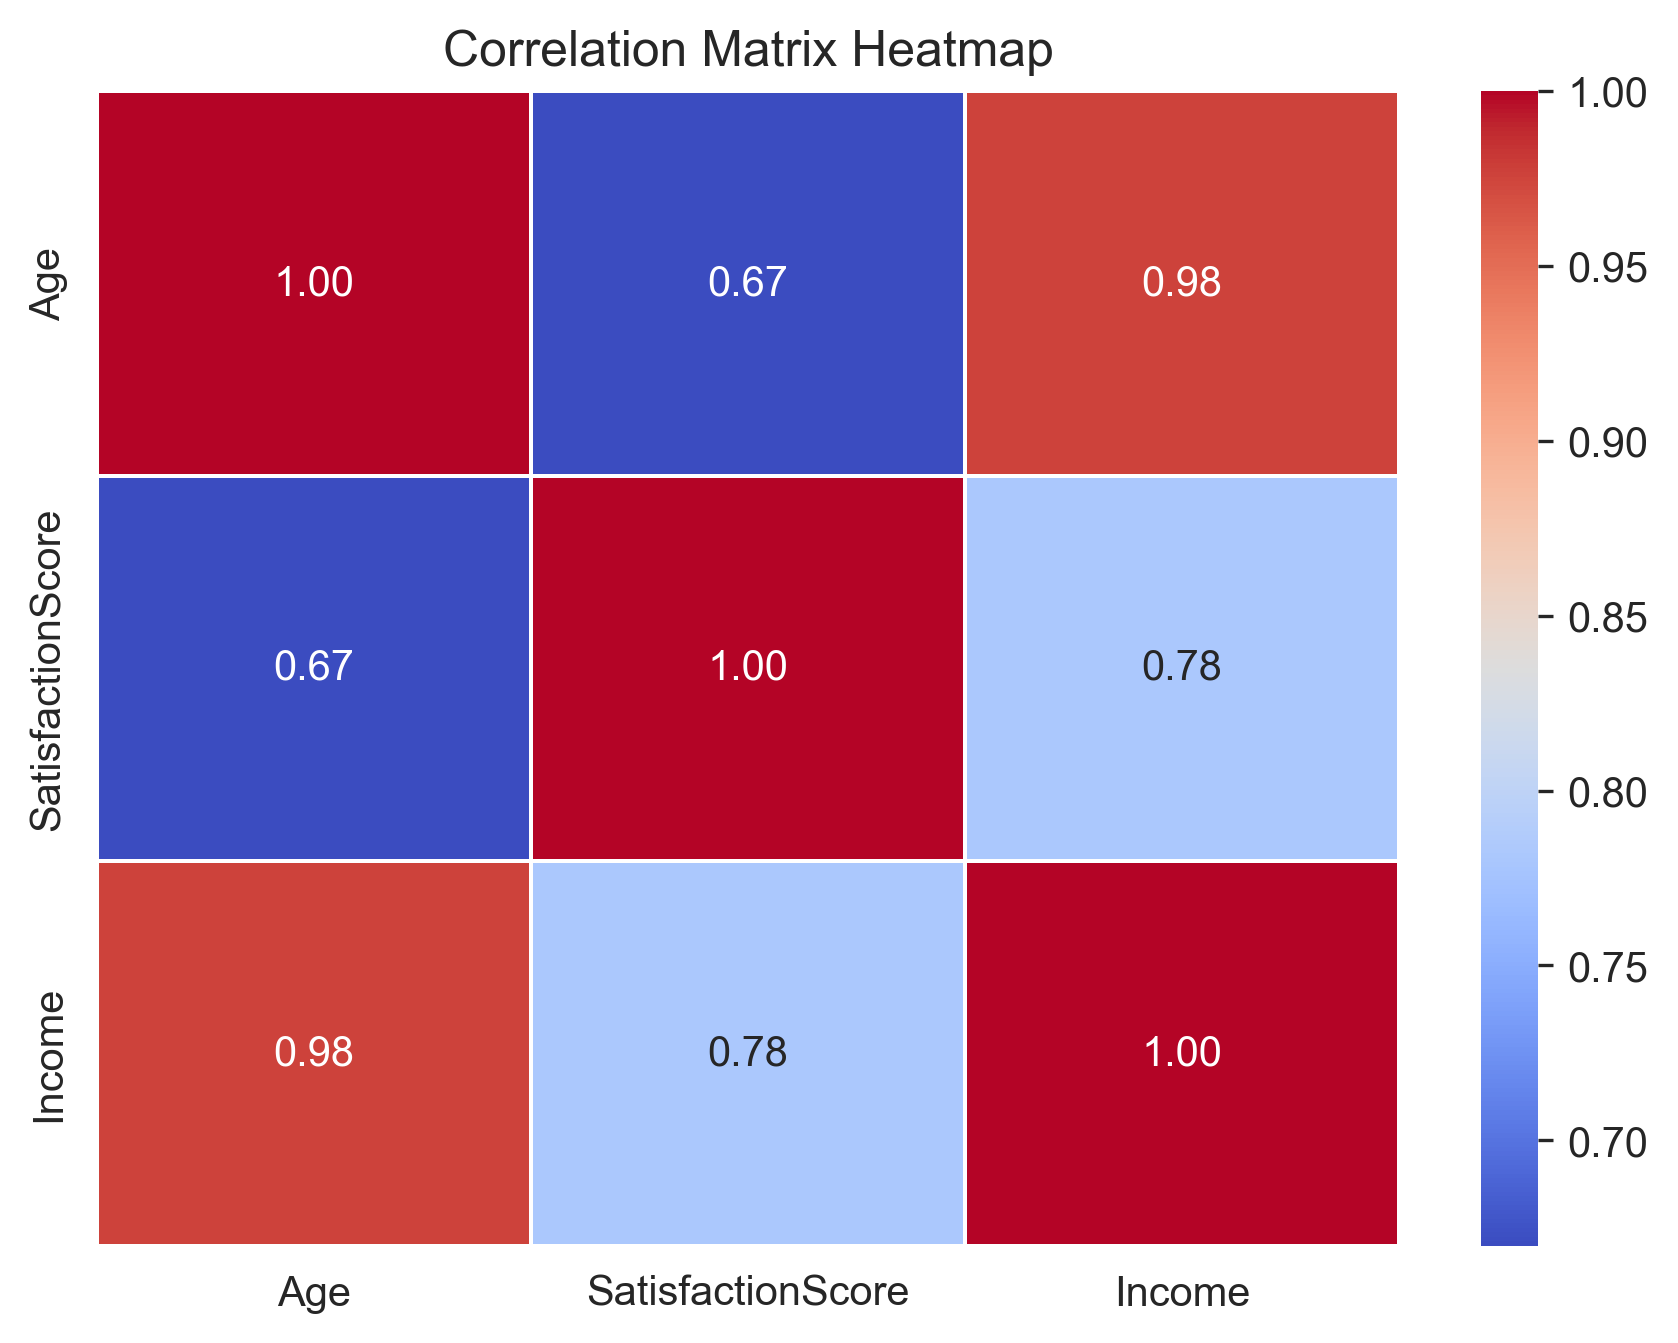
\includegraphics[keepaspectratio]{02-data-handling-exploration_files/figure-latex/cell-48-output-1.png}}

\begin{verbatim}
* **해석:** 색상의 진하기나 종류를 통해 변수 간 상관관계의 강도와 방향(양/음)을 시각적으로 파악할 수 있습니다. (상관계수 자체에 대한 자세한 내용은 5장에서 다룹니다.)
\end{verbatim}

\subsection{2.4.4 그래프 꾸미기 및 저장 (Customization and Saving
Plots)}\label{uxadf8uxb798uxd504-uxafb8uxbbf8uxae30-uxbc0f-uxc800uxc7a5-customization-and-saving-plots}

Matplotlib와 Seaborn은 그래프의 제목, 축 레이블, 범례, 색상, 폰트 크기
등 다양한 요소를 사용자가 원하는 대로 조정할 수 있는 기능을 제공합니다.

\begin{itemize}
\tightlist
\item
  \textbf{주요 꾸미기 함수:}

  \begin{itemize}
  \tightlist
  \item
    \texttt{plt.title()}: 그래프 제목 설정
  \item
    \texttt{plt.xlabel()}, \texttt{plt.ylabel()}: x축, y축 레이블 설정
  \item
    \texttt{plt.xticks()}, \texttt{plt.yticks()}: 축 눈금 설정 (값,
    레이블, 회전 등)
  \item
    \texttt{plt.legend()}: 범례 표시 및 위치/스타일 조정
  \item
    \texttt{plt.grid()}: 그리드(격자) 표시
  \item
    \texttt{plt.figure(figsize=(width,\ height))}: 그래프 크기 조절
  \item
    \texttt{plt.tight\_layout()}: 그래프 요소들이 겹치지 않게 자동으로
    레이아웃 조정
  \end{itemize}
\item
  \textbf{그래프 저장:}

  \begin{itemize}
  \tightlist
  \item
    \texttt{plt.savefig(\textquotesingle{}filename.png\textquotesingle{},\ dpi=300)}:
    생성된 그래프를 파일로 저장합니다. 파일 형식(png, jpg, pdf 등)과
    해상도(dpi)를 지정할 수 있습니다. 논문이나 보고서에 삽입할 때
    유용합니다.
  \end{itemize}
\end{itemize}

\begin{Shaded}
\begin{Highlighting}[]
\CommentTok{\# 예시: 꾸미기가 적용된 그래프 저장}
\NormalTok{plt.figure(figsize}\OperatorTok{=}\NormalTok{(}\DecValTok{8}\NormalTok{, }\DecValTok{6}\NormalTok{))}
\NormalTok{sns.scatterplot(data}\OperatorTok{=}\NormalTok{df\_survey, x}\OperatorTok{=}\StringTok{\textquotesingle{}Age\textquotesingle{}}\NormalTok{, y}\OperatorTok{=}\StringTok{\textquotesingle{}Income\textquotesingle{}}\NormalTok{, hue}\OperatorTok{=}\StringTok{\textquotesingle{}Gender\textquotesingle{}}\NormalTok{)}
\NormalTok{plt.title(}\StringTok{\textquotesingle{}Age vs Income Scatter Plot with Customization\textquotesingle{}}\NormalTok{, fontsize}\OperatorTok{=}\DecValTok{16}\NormalTok{)}
\NormalTok{plt.xlabel(}\StringTok{\textquotesingle{}Age (Years)\textquotesingle{}}\NormalTok{, fontsize}\OperatorTok{=}\DecValTok{12}\NormalTok{)}
\NormalTok{plt.ylabel(}\StringTok{\textquotesingle{}Income ($)\textquotesingle{}}\NormalTok{, fontsize}\OperatorTok{=}\DecValTok{12}\NormalTok{)}
\NormalTok{plt.legend(title}\OperatorTok{=}\StringTok{\textquotesingle{}Gender\textquotesingle{}}\NormalTok{, title\_fontsize}\OperatorTok{=}\StringTok{\textquotesingle{}13\textquotesingle{}}\NormalTok{, fontsize}\OperatorTok{=}\StringTok{\textquotesingle{}11\textquotesingle{}}\NormalTok{)}
\NormalTok{plt.grid(}\VariableTok{True}\NormalTok{, linestyle}\OperatorTok{=}\StringTok{\textquotesingle{}{-}{-}\textquotesingle{}}\NormalTok{, alpha}\OperatorTok{=}\FloatTok{0.7}\NormalTok{) }\CommentTok{\# 그리드 추가}

\CommentTok{\# 파일로 저장 (plt.show() 이전에 호출해야 할 수 있음)}
\CommentTok{\# plt.savefig(\textquotesingle{}age\_income\_scatter.png\textquotesingle{}, dpi=300, bbox\_inches=\textquotesingle{}tight\textquotesingle{}) \# bbox\_inches=\textquotesingle{}tight\textquotesingle{}는 여백 최소화}

\NormalTok{plt.show()}
\end{Highlighting}
\end{Shaded}

\pandocbounded{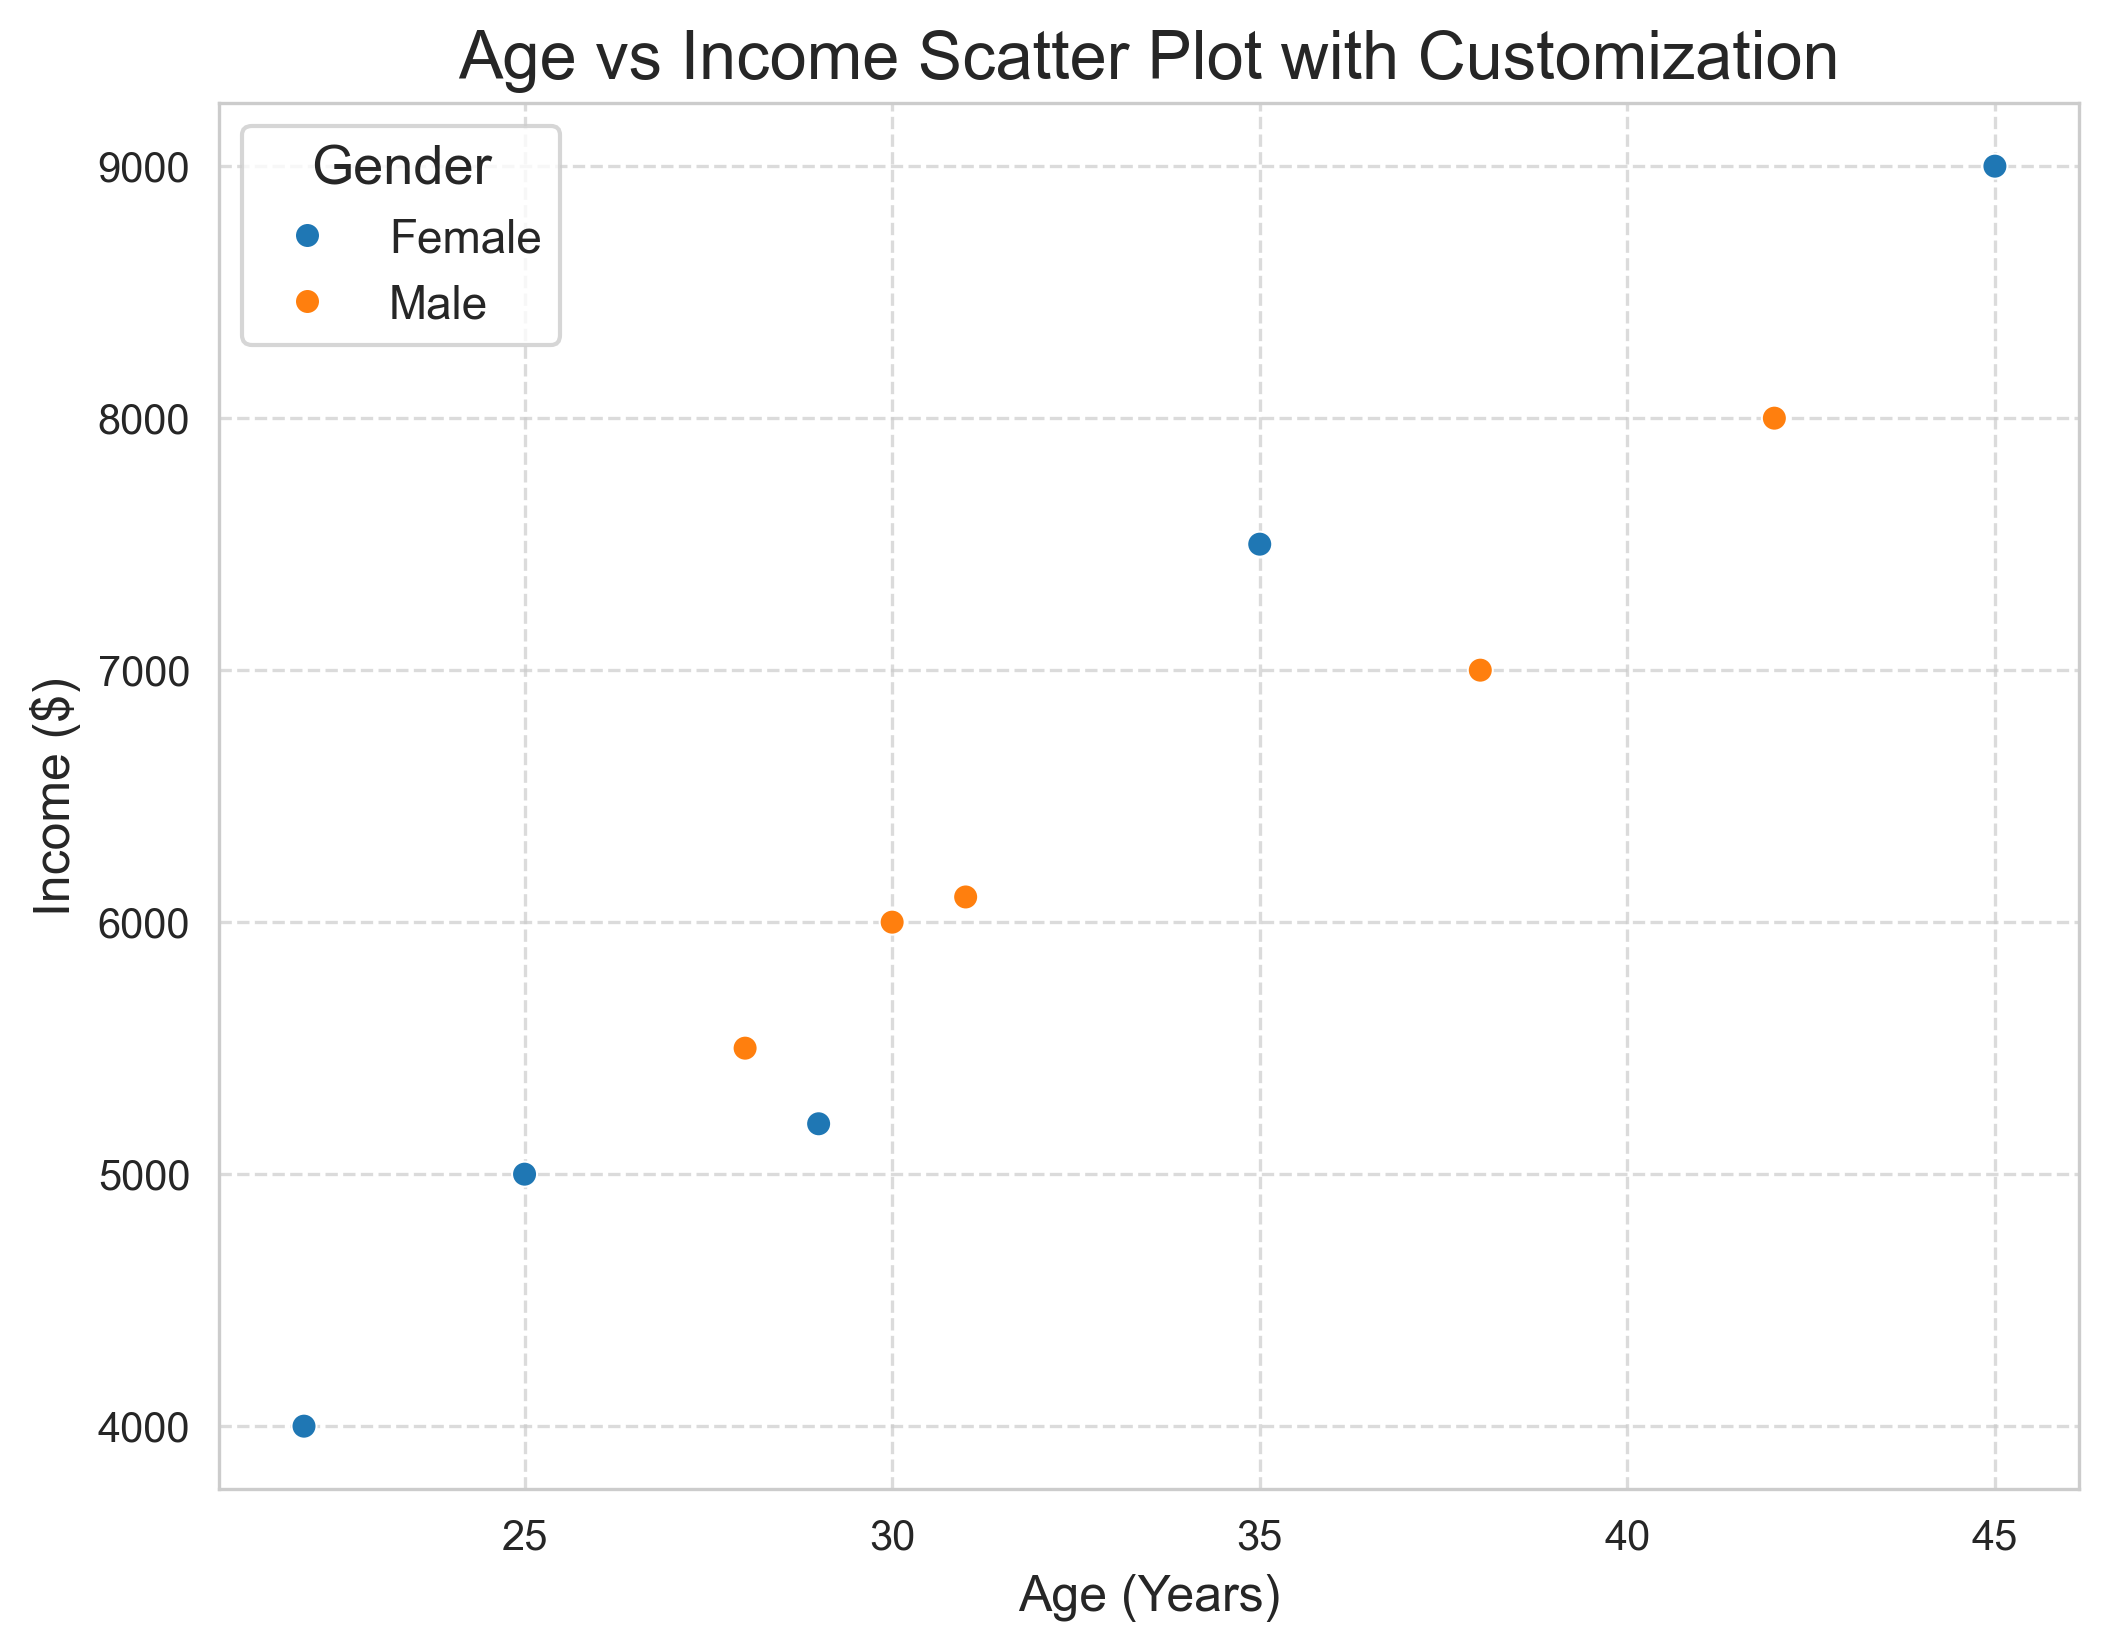
\includegraphics[keepaspectratio]{02-data-handling-exploration_files/figure-latex/cell-49-output-1.png}}

\subsection{2.4.5 데이터 시각화의
중요성}\label{uxb370uxc774uxd130-uxc2dcuxac01uxd654uxc758-uxc911uxc694uxc131}

데이터 시각화는 기술 통계량만으로는 파악하기 어려운 데이터의 복잡한
패턴과 구조를 드러내 줍니다. 효과적인 시각화는 데이터 탐색 과정을
풍부하게 하고, 분석 결과에 대한 설득력을 높이며, 연구 아이디어를
발전시키는 데 기여합니다. 사회과학 연구자는 연구 목적과 데이터 유형에
맞는 적절한 시각화 방법을 선택하고, 그 결과를 비판적으로 해석하는 능력을
갖추는 것이 중요합니다.

여기까지 파이썬을 이용한 데이터 핸들링, 전처리, 기술 통계 분석, 그리고
시각화 기초를 다루었습니다. 다음 장부터는 이러한 기초를 바탕으로
본격적인 통계 분석 기법들을 학습하게 됩니다.

\section{2.5 실전 연습: 설문조사 데이터 종합 분석 및
해석}\label{sec-chapter2-practice}

이번 장에서 우리는 파이썬을 활용한 데이터 분석의 여정을 시작하여,
Pandas를 이용한 데이터 조작, 데이터 정제(전처리), 기술 통계량 계산,
그리고 Matplotlib와 Seaborn을 활용한 시각화 기법들을 학습했습니다.
이론과 개별 기능 학습도 중요하지만, 실제 분석 과정에서는 이러한 기법들이
유기적으로 연결되어 사용됩니다.

본 절에서는 \textbf{2장에서 배운 모든 지식을 총동원}하여, 조금 더
현실적인 규모(100명 응답자)의 가상 설문조사 데이터를 직접 다루어보는
종합 실습을 진행합니다. 단순히 코드를 실행하는 것을 넘어, 각 분석 단계의
\textbf{필요성}을 이해하고 도출된 결과(수치, 그래프)가 가지는
\textbf{통계적 의미}와 \textbf{사회과학적 함의}를 해석하는 데 중점을 둘
것입니다. 이 과정을 통해 여러분은 실제 연구 데이터를 만났을 때 필요한
데이터 탐색 및 기초 분석 능력을 통합적으로 강화할 수 있습니다.

\begin{tcolorbox}[enhanced jigsaw, bottomtitle=1mm, colbacktitle=quarto-callout-note-color!10!white, rightrule=.15mm, colback=white, leftrule=.75mm, toptitle=1mm, titlerule=0mm, opacityback=0, opacitybacktitle=0.6, left=2mm, title=\textcolor{quarto-callout-note-color}{\faInfo}\hspace{0.5em}{📌 핵심 목표}, breakable, bottomrule=.15mm, arc=.35mm, colframe=quarto-callout-note-color-frame, toprule=.15mm, coltitle=black]

\begin{itemize}
\tightlist
\item
  100명 규모의 가상 설문조사 데이터를 생성하고 구조를 파악합니다.
\item
  2.2절에서 배운 기법을 활용하여 결측치, 이상치 등 데이터 문제를
  식별하고 처리합니다. (데이터 전처리)
\item
  2.3절에서 배운 기법을 활용하여 데이터의 중심 경향성, 산포도, 분포
  특성을 계산하고 통계적으로 해석합니다. (기술 통계 분석)
\item
  2.4절에서 배운 기법을 활용하여 변수 분포 및 변수 간 관계를 시각화하고
  패턴을 탐색합니다. (데이터 시각화)
\item
  분석 전 과정의 결과를 종합하여 데이터에 대한 깊이 있는 이해를
  도출하고, 사회과학적 맥락에서 의미를 해석하는 연습을 합니다.
\end{itemize}

\end{tcolorbox}

\subsection{2.5.1 실습용 가상 데이터 생성
(N=100)}\label{uxc2e4uxc2b5uxc6a9-uxac00uxc0c1-uxb370uxc774uxd130-uxc0dduxc131-n100}

먼저, 실습에 사용할 100명의 응답자 데이터를 포함하는 가상 설문조사
DataFrame(\texttt{df\_practice})을 생성하겠습니다. 이전 예제보다
현실성을 높이기 위해 변수 값 생성 시 약간의 무작위성과 함께 결측치,
그리고 잠재적 이상치를 포함시키겠습니다.

\begin{Shaded}
\begin{Highlighting}[]
\ImportTok{import}\NormalTok{ pandas }\ImportTok{as}\NormalTok{ pd}
\ImportTok{import}\NormalTok{ numpy }\ImportTok{as}\NormalTok{ np}
\ImportTok{import}\NormalTok{ matplotlib.pyplot }\ImportTok{as}\NormalTok{ plt}
\ImportTok{import}\NormalTok{ seaborn }\ImportTok{as}\NormalTok{ sns}

\CommentTok{\# 재현 가능성을 위한 시드 설정}
\NormalTok{np.random.seed(}\DecValTok{42}\NormalTok{)}

\CommentTok{\# 데이터 생성 (N=100)}
\NormalTok{n\_respondents }\OperatorTok{=} \DecValTok{100}
\NormalTok{data }\OperatorTok{=}\NormalTok{ \{}
    \StringTok{\textquotesingle{}ID\textquotesingle{}}\NormalTok{: }\BuiltInTok{range}\NormalTok{(}\DecValTok{1}\NormalTok{, n\_respondents }\OperatorTok{+} \DecValTok{1}\NormalTok{),}
    \StringTok{\textquotesingle{}Age\textquotesingle{}}\NormalTok{: np.random.randint(}\DecValTok{20}\NormalTok{, }\DecValTok{65}\NormalTok{, size}\OperatorTok{=}\NormalTok{n\_respondents),}
    \StringTok{\textquotesingle{}Gender\textquotesingle{}}\NormalTok{: np.random.choice([}\StringTok{\textquotesingle{}Male\textquotesingle{}}\NormalTok{, }\StringTok{\textquotesingle{}Female\textquotesingle{}}\NormalTok{], size}\OperatorTok{=}\NormalTok{n\_respondents, p}\OperatorTok{=}\NormalTok{[}\FloatTok{0.48}\NormalTok{, }\FloatTok{0.52}\NormalTok{]),}
    \StringTok{\textquotesingle{}Education\textquotesingle{}}\NormalTok{: np.random.choice([}\StringTok{\textquotesingle{}High School\textquotesingle{}}\NormalTok{, }\StringTok{\textquotesingle{}Bachelor\textquotesingle{}}\NormalTok{, }\StringTok{\textquotesingle{}Master\textquotesingle{}}\NormalTok{, }\StringTok{\textquotesingle{}PhD\textquotesingle{}}\NormalTok{], size}\OperatorTok{=}\NormalTok{n\_respondents, p}\OperatorTok{=}\NormalTok{[}\FloatTok{0.2}\NormalTok{, }\FloatTok{0.4}\NormalTok{, }\FloatTok{0.3}\NormalTok{, }\FloatTok{0.1}\NormalTok{]),}
    \StringTok{\textquotesingle{}Income\textquotesingle{}}\NormalTok{: np.random.normal(loc}\OperatorTok{=}\DecValTok{5500}\NormalTok{, scale}\OperatorTok{=}\DecValTok{1500}\NormalTok{, size}\OperatorTok{=}\NormalTok{n\_respondents).}\BuiltInTok{round}\NormalTok{(}\DecValTok{2}\NormalTok{),}
    \StringTok{\textquotesingle{}Wellbeing\textquotesingle{}}\NormalTok{: np.random.normal(loc}\OperatorTok{=}\FloatTok{6.5}\NormalTok{, scale}\OperatorTok{=}\FloatTok{1.8}\NormalTok{, size}\OperatorTok{=}\NormalTok{n\_respondents).}\BuiltInTok{round}\NormalTok{(}\DecValTok{1}\NormalTok{),}
    \StringTok{\textquotesingle{}Social\_Participation\textquotesingle{}}\NormalTok{: np.random.randint(}\DecValTok{1}\NormalTok{, }\DecValTok{6}\NormalTok{, size}\OperatorTok{=}\NormalTok{n\_respondents), }\CommentTok{\# 1(낮음)\textasciitilde{}5(높음)}
    \StringTok{\textquotesingle{}Political\_View\textquotesingle{}}\NormalTok{: np.random.randint(}\DecValTok{1}\NormalTok{, }\DecValTok{8}\NormalTok{, size}\OperatorTok{=}\NormalTok{n\_respondents) }\CommentTok{\# 1(진보)\textasciitilde{}7(보수)}
\NormalTok{\}}
\NormalTok{df\_practice }\OperatorTok{=}\NormalTok{ pd.DataFrame(data)}

\CommentTok{\# 의도적으로 결측치(NaN) 추가}
\NormalTok{nan\_indices\_income }\OperatorTok{=}\NormalTok{ np.random.choice(df\_practice.index, size}\OperatorTok{=}\DecValTok{8}\NormalTok{, replace}\OperatorTok{=}\VariableTok{False}\NormalTok{)}
\NormalTok{df\_practice.loc[nan\_indices\_income, }\StringTok{\textquotesingle{}Income\textquotesingle{}}\NormalTok{] }\OperatorTok{=}\NormalTok{ np.nan}

\NormalTok{nan\_indices\_wellbeing }\OperatorTok{=}\NormalTok{ np.random.choice(df\_practice.index, size}\OperatorTok{=}\DecValTok{5}\NormalTok{, replace}\OperatorTok{=}\VariableTok{False}\NormalTok{)}
\NormalTok{df\_practice.loc[nan\_indices\_wellbeing, }\StringTok{\textquotesingle{}Wellbeing\textquotesingle{}}\NormalTok{] }\OperatorTok{=}\NormalTok{ np.nan}

\CommentTok{\# 의도적으로 이상치 추가 (예: Age, Income)}
\NormalTok{df\_practice.loc[np.random.choice(df\_practice.index, }\DecValTok{1}\NormalTok{), }\StringTok{\textquotesingle{}Age\textquotesingle{}}\NormalTok{] }\OperatorTok{=} \DecValTok{99}
\NormalTok{df\_practice.loc[np.random.choice(df\_practice.index, }\DecValTok{1}\NormalTok{), }\StringTok{\textquotesingle{}Income\textquotesingle{}}\NormalTok{] }\OperatorTok{=} \FloatTok{15000.0}

\CommentTok{\# Education을 순서형 범주로 변환 (선택적이지만, 분석/시각화 시 순서 고려에 유용)}
\NormalTok{edu\_order }\OperatorTok{=}\NormalTok{ [}\StringTok{\textquotesingle{}High School\textquotesingle{}}\NormalTok{, }\StringTok{\textquotesingle{}Bachelor\textquotesingle{}}\NormalTok{, }\StringTok{\textquotesingle{}Master\textquotesingle{}}\NormalTok{, }\StringTok{\textquotesingle{}PhD\textquotesingle{}}\NormalTok{]}
\NormalTok{df\_practice[}\StringTok{\textquotesingle{}Education\textquotesingle{}}\NormalTok{] }\OperatorTok{=}\NormalTok{ pd.Categorical(df\_practice[}\StringTok{\textquotesingle{}Education\textquotesingle{}}\NormalTok{], categories}\OperatorTok{=}\NormalTok{edu\_order, ordered}\OperatorTok{=}\VariableTok{True}\NormalTok{)}

\BuiltInTok{print}\NormalTok{(}\StringTok{"{-}{-}{-} 가상 설문 데이터 생성 완료 (N=100) {-}{-}{-}"}\NormalTok{)}
\BuiltInTok{print}\NormalTok{(}\StringTok{"데이터 샘플 (처음 5행):"}\NormalTok{)}
\BuiltInTok{print}\NormalTok{(df\_practice.head())}
\end{Highlighting}
\end{Shaded}

\begin{verbatim}
--- 가상 설문 데이터 생성 완료 (N=100) ---
데이터 샘플 (처음 5행):
   ID  Age  Gender    Education   Income  Wellbeing  Social_Participation  \
0   1   58  Female  High School  4666.08        4.1                     2   
1   2   48  Female          PhD  5308.40        0.4                     4   
2   3   34  Female     Bachelor  3159.16        8.5                     2   
3   4   62  Female     Bachelor  8500.52       10.4                     2   
4   5   27  Female       Master  3699.80        5.9                     2   

   Political_View  
0               7  
1               6  
2               2  
3               5  
4               2  
\end{verbatim}

\subsection{2.5.2 데이터 탐색 및 전처리 (2.1 \& 2.2
적용)}\label{uxb370uxc774uxd130-uxd0d0uxc0c9-uxbc0f-uxc804uxcc98uxb9ac-2.1-2.2-uxc801uxc6a9}

생성된 데이터를 분석하기 전에 데이터의 구조를 파악하고 잠재적인 문제점을
해결하는 전처리 과정을 거쳐야 합니다.

\textbf{1. 기본 정보 확인:}

\begin{Shaded}
\begin{Highlighting}[]
\BuiltInTok{print}\NormalTok{(}\StringTok{"}\CharTok{\textbackslash{}n}\StringTok{{-}{-}{-} 데이터 기본 정보 (.info()) {-}{-}{-}"}\NormalTok{)}
\NormalTok{df\_practice.info()}
\end{Highlighting}
\end{Shaded}

\begin{verbatim}

--- 데이터 기본 정보 (.info()) ---
<class 'pandas.core.frame.DataFrame'>
RangeIndex: 100 entries, 0 to 99
Data columns (total 8 columns):
 #   Column                Non-Null Count  Dtype   
---  ------                --------------  -----   
 0   ID                    100 non-null    int64   
 1   Age                   100 non-null    int32   
 2   Gender                100 non-null    object  
 3   Education             100 non-null    category
 4   Income                92 non-null     float64 
 5   Wellbeing             95 non-null     float64 
 6   Social_Participation  100 non-null    int32   
 7   Political_View        100 non-null    int32   
dtypes: category(1), float64(2), int32(3), int64(1), object(1)
memory usage: 4.7+ KB
\end{verbatim}

\begin{itemize}
\tightlist
\item
  \textbf{해석:} \texttt{.info()} 결과는 100개의 행(Entries)과 8개의
  열(Columns)이 있음을 보여줍니다. 각 열의 데이터 타입과 non-null 개수를
  확인할 수 있습니다. \texttt{Income}과 \texttt{Wellbeing} 열에서
  non-null 개수가 100보다 적으므로 결측치가 존재함을 알 수 있습니다.
  \texttt{Education}은 \texttt{CategoricalDtype}으로 올바르게
  인식되었습니다.
\end{itemize}

\textbf{2. 결측치 확인 및 처리:}

\begin{Shaded}
\begin{Highlighting}[]
\BuiltInTok{print}\NormalTok{(}\StringTok{"}\CharTok{\textbackslash{}n}\StringTok{{-}{-}{-} 결측치 개수 확인 (.isnull().sum()) {-}{-}{-}"}\NormalTok{)}
\BuiltInTok{print}\NormalTok{(df\_practice.isnull().}\BuiltInTok{sum}\NormalTok{())}
\end{Highlighting}
\end{Shaded}

\begin{verbatim}

--- 결측치 개수 확인 (.isnull().sum()) ---
ID                      0
Age                     0
Gender                  0
Education               0
Income                  8
Wellbeing               5
Social_Participation    0
Political_View          0
dtype: int64
\end{verbatim}

\begin{itemize}
\tightlist
\item
  \textbf{해석:} \texttt{Income} 열에 8개, \texttt{Wellbeing} 열에 5개의
  결측치가 확인됩니다. 이 결측치를 어떻게 처리할지 결정해야 합니다. 처리
  방법은 데이터의 특성, 결측치의 양, 분석 목적에 따라 달라집니다.
\item
  \textbf{처리 전략 및 실행:}

  \begin{itemize}
  \tightlist
  \item
    \texttt{Income}: 소득 데이터는 종종 오른쪽으로 치우친 분포(소수의
    고소득자)를 가집니다. 이 경우 평균(mean)보다는 중앙값(median)으로
    대체하는 것이 전체 분포를 덜 왜곡시킬 수 있습니다.
  \item
    \texttt{Wellbeing}: 웰빙 점수는 주관적 응답이며 5개의 결측치는 전체
    데이터의 5\%입니다. 이 정도면 해당 응답을 분석에서 제외(행 삭제)하는
    것도 고려할 수 있으나, 여기서는 \texttt{Income}과 마찬가지로
    중앙값으로 대체해보겠습니다. (실제 분석에서는 삭제, 대체, 예측 모델
    사용 등 다양한 방법의 장단점을 고려해야 합니다.)
  \end{itemize}
\end{itemize}

\begin{Shaded}
\begin{Highlighting}[]
\CommentTok{\# Income 결측치를 중앙값으로 대체}
\NormalTok{income\_median }\OperatorTok{=}\NormalTok{ df\_practice[}\StringTok{\textquotesingle{}Income\textquotesingle{}}\NormalTok{].median()}
\NormalTok{df\_practice[}\StringTok{\textquotesingle{}Income\textquotesingle{}}\NormalTok{].fillna(income\_median, inplace}\OperatorTok{=}\VariableTok{True}\NormalTok{)}
\BuiltInTok{print}\NormalTok{(}\SpecialStringTok{f"}\CharTok{\textbackslash{}n}\SpecialStringTok{Income 결측치를 중앙값 (}\SpecialCharTok{\{}\NormalTok{income\_median}\SpecialCharTok{\}}\SpecialStringTok{)으로 대체 완료."}\NormalTok{)}

\CommentTok{\# Wellbeing 결측치를 중앙값으로 대체}
\NormalTok{wellbeing\_median }\OperatorTok{=}\NormalTok{ df\_practice[}\StringTok{\textquotesingle{}Wellbeing\textquotesingle{}}\NormalTok{].median()}
\NormalTok{df\_practice[}\StringTok{\textquotesingle{}Wellbeing\textquotesingle{}}\NormalTok{].fillna(wellbeing\_median, inplace}\OperatorTok{=}\VariableTok{True}\NormalTok{)}
\BuiltInTok{print}\NormalTok{(}\SpecialStringTok{f"Wellbeing 결측치를 중앙값 (}\SpecialCharTok{\{}\NormalTok{wellbeing\_median}\SpecialCharTok{\}}\SpecialStringTok{)으로 대체 완료."}\NormalTok{)}

\CommentTok{\# 결측치 처리 결과 확인}
\BuiltInTok{print}\NormalTok{(}\StringTok{"}\CharTok{\textbackslash{}n}\StringTok{{-}{-}{-} 결측치 처리 후 확인 (.isnull().sum()) {-}{-}{-}"}\NormalTok{)}
\BuiltInTok{print}\NormalTok{(df\_practice.isnull().}\BuiltInTok{sum}\NormalTok{())}
\end{Highlighting}
\end{Shaded}

\begin{verbatim}

Income 결측치를 중앙값 (5628.05)으로 대체 완료.
Wellbeing 결측치를 중앙값 (6.1)으로 대체 완료.

--- 결측치 처리 후 확인 (.isnull().sum()) ---
ID                      0
Age                     0
Gender                  0
Education               0
Income                  0
Wellbeing               0
Social_Participation    0
Political_View          0
dtype: int64
\end{verbatim}

\begin{verbatim}
C:\Users\voidm\AppData\Local\Temp\ipykernel_34588\4130031253.py:3: FutureWarning:

A value is trying to be set on a copy of a DataFrame or Series through chained assignment using an inplace method.
The behavior will change in pandas 3.0. This inplace method will never work because the intermediate object on which we are setting values always behaves as a copy.

For example, when doing 'df[col].method(value, inplace=True)', try using 'df.method({col: value}, inplace=True)' or df[col] = df[col].method(value) instead, to perform the operation inplace on the original object.



C:\Users\voidm\AppData\Local\Temp\ipykernel_34588\4130031253.py:8: FutureWarning:

A value is trying to be set on a copy of a DataFrame or Series through chained assignment using an inplace method.
The behavior will change in pandas 3.0. This inplace method will never work because the intermediate object on which we are setting values always behaves as a copy.

For example, when doing 'df[col].method(value, inplace=True)', try using 'df.method({col: value}, inplace=True)' or df[col] = df[col].method(value) instead, to perform the operation inplace on the original object.


\end{verbatim}

\textbf{3. 이상치 탐지 및 처리:}

\begin{itemize}
\tightlist
\item
  \textbf{탐지:} 수치형 변수인 \texttt{Age}와 \texttt{Income}에 대해
  이상치가 있는지 박스 플롯(Box Plot)으로 시각적으로 확인하고, IQR
  기준으로도 탐지해 보겠습니다.
\end{itemize}

\begin{Shaded}
\begin{Highlighting}[]
\CommentTok{\# Age와 Income에 대한 박스 플롯}
\NormalTok{plt.figure(figsize}\OperatorTok{=}\NormalTok{(}\DecValTok{10}\NormalTok{, }\DecValTok{5}\NormalTok{))}
\NormalTok{plt.subplot(}\DecValTok{1}\NormalTok{, }\DecValTok{2}\NormalTok{, }\DecValTok{1}\NormalTok{) }\CommentTok{\# 1행 2열 중 첫 번째}
\NormalTok{sns.boxplot(y}\OperatorTok{=}\NormalTok{df\_practice[}\StringTok{\textquotesingle{}Age\textquotesingle{}}\NormalTok{])}
\NormalTok{plt.title(}\StringTok{\textquotesingle{}Box Plot of Age\textquotesingle{}}\NormalTok{)}

\NormalTok{plt.subplot(}\DecValTok{1}\NormalTok{, }\DecValTok{2}\NormalTok{, }\DecValTok{2}\NormalTok{) }\CommentTok{\# 1행 2열 중 두 번째}
\NormalTok{sns.boxplot(y}\OperatorTok{=}\NormalTok{df\_practice[}\StringTok{\textquotesingle{}Income\textquotesingle{}}\NormalTok{])}
\NormalTok{plt.title(}\StringTok{\textquotesingle{}Box Plot of Income\textquotesingle{}}\NormalTok{)}

\NormalTok{plt.tight\_layout()}
\NormalTok{plt.show()}

\CommentTok{\# IQR 기반 이상치 탐지 함수 정의 (2.2절 내용 활용)}
\KeywordTok{def}\NormalTok{ detect\_outliers\_iqr(df, column):}
\NormalTok{    Q1 }\OperatorTok{=}\NormalTok{ df[column].quantile(}\FloatTok{0.25}\NormalTok{)}
\NormalTok{    Q3 }\OperatorTok{=}\NormalTok{ df[column].quantile(}\FloatTok{0.75}\NormalTok{)}
\NormalTok{    IQR }\OperatorTok{=}\NormalTok{ Q3 }\OperatorTok{{-}}\NormalTok{ Q1}
\NormalTok{    lower\_bound }\OperatorTok{=}\NormalTok{ Q1 }\OperatorTok{{-}} \FloatTok{1.5} \OperatorTok{*}\NormalTok{ IQR}
\NormalTok{    upper\_bound }\OperatorTok{=}\NormalTok{ Q3 }\OperatorTok{+} \FloatTok{1.5} \OperatorTok{*}\NormalTok{ IQR}
\NormalTok{    outliers }\OperatorTok{=}\NormalTok{ df[(df[column] }\OperatorTok{\textless{}}\NormalTok{ lower\_bound) }\OperatorTok{|}\NormalTok{ (df[column] }\OperatorTok{\textgreater{}}\NormalTok{ upper\_bound)]}
    \ControlFlowTok{return}\NormalTok{ outliers, lower\_bound, upper\_bound}

\CommentTok{\# Age 이상치 탐지}
\NormalTok{age\_outliers, age\_lower, age\_upper }\OperatorTok{=}\NormalTok{ detect\_outliers\_iqr(df\_practice, }\StringTok{\textquotesingle{}Age\textquotesingle{}}\NormalTok{)}
\BuiltInTok{print}\NormalTok{(}\StringTok{"}\CharTok{\textbackslash{}n}\StringTok{{-}{-}{-} Age Outliers (IQR method) {-}{-}{-}"}\NormalTok{)}
\BuiltInTok{print}\NormalTok{(age\_outliers)}
\BuiltInTok{print}\NormalTok{(}\SpecialStringTok{f"Age lower bound: }\SpecialCharTok{\{}\NormalTok{age\_lower}\SpecialCharTok{:.2f\}}\SpecialStringTok{, upper bound: }\SpecialCharTok{\{}\NormalTok{age\_upper}\SpecialCharTok{:.2f\}}\SpecialStringTok{"}\NormalTok{)}

\CommentTok{\# Income 이상치 탐지}
\NormalTok{income\_outliers, income\_lower, income\_upper }\OperatorTok{=}\NormalTok{ detect\_outliers\_iqr(df\_practice, }\StringTok{\textquotesingle{}Income\textquotesingle{}}\NormalTok{)}
\BuiltInTok{print}\NormalTok{(}\StringTok{"}\CharTok{\textbackslash{}n}\StringTok{{-}{-}{-} Income Outliers (IQR method) {-}{-}{-}"}\NormalTok{)}
\BuiltInTok{print}\NormalTok{(income\_outliers)}
\BuiltInTok{print}\NormalTok{(}\SpecialStringTok{f"Income lower bound: }\SpecialCharTok{\{}\NormalTok{income\_lower}\SpecialCharTok{:.2f\}}\SpecialStringTok{, upper bound: }\SpecialCharTok{\{}\NormalTok{income\_upper}\SpecialCharTok{:.2f\}}\SpecialStringTok{"}\NormalTok{)}
\end{Highlighting}
\end{Shaded}

\pandocbounded{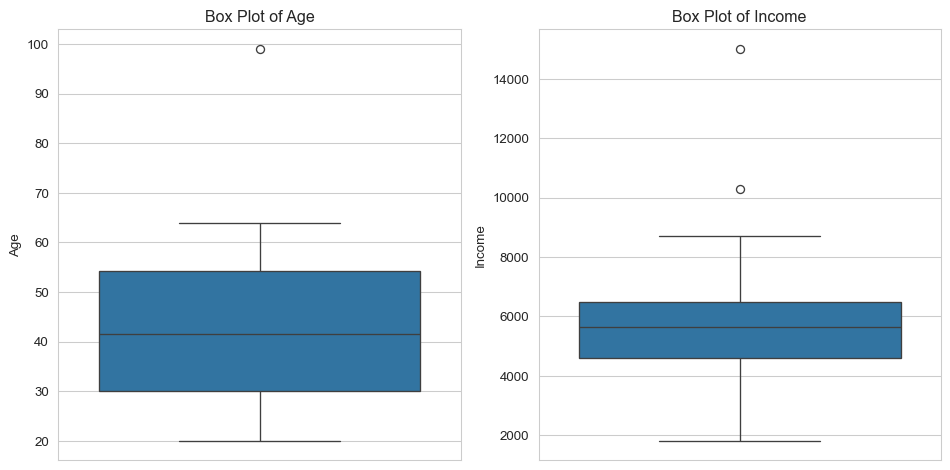
\includegraphics[keepaspectratio]{02-data-handling-exploration_files/figure-latex/cell-54-output-1.png}}

\begin{verbatim}

--- Age Outliers (IQR method) ---
   ID  Age Gender Education   Income  Wellbeing  Social_Participation  \
8   9   99   Male  Bachelor  6031.63        8.1                     4   

   Political_View  
8               7  
Age lower bound: -6.38, upper bound: 90.62

--- Income Outliers (IQR method) ---
    ID  Age  Gender Education    Income  Wellbeing  Social_Participation  \
44  45   33  Female    Master  10280.55        8.9                     5   
73  74   27    Male  Bachelor  15000.00        3.4                     5   

    Political_View  
44               1  
73               6  
Income lower bound: 1726.57, upper bound: 9361.88
\end{verbatim}

\begin{itemize}
\tightlist
\item
  \textbf{해석:} \texttt{Age}의 박스 플롯과 IQR 기준 탐지에서 99세가
  명확한 이상치로 나타납니다. 이는 데이터 생성 시 의도적으로 넣은
  값입니다. \texttt{Income}에서도 상단에 이상치(15000)가 확인됩니다.
\item
  \textbf{처리 전략 및 실행:}

  \begin{itemize}
  \tightlist
  \item
    \texttt{Age}: 99세는 현실적으로 가능성이 낮은 연령이거나 오류일 수
    있습니다. 이를 분석 목적에 따라 제외하거나, 상한값(e.g.,
    upper\_bound)으로 조정(Clipping/Winsorizing)할 수 있습니다. 여기서는
    상한값으로 조정해보겠습니다.
  \item
    \texttt{Income}: 15000 소득 역시 다른 값들에 비해 매우 높습니다. 이
    역시 상한값으로 조정하여 극단치의 영향을 줄이겠습니다.
  \end{itemize}
\end{itemize}

\begin{Shaded}
\begin{Highlighting}[]
\CommentTok{\# Age 이상치를 상한값으로 조정 (Clipping)}
\NormalTok{df\_practice[}\StringTok{\textquotesingle{}Age\textquotesingle{}}\NormalTok{] }\OperatorTok{=}\NormalTok{ df\_practice[}\StringTok{\textquotesingle{}Age\textquotesingle{}}\NormalTok{].clip(upper}\OperatorTok{=}\NormalTok{age\_upper)}
\BuiltInTok{print}\NormalTok{(}\SpecialStringTok{f"}\CharTok{\textbackslash{}n}\SpecialStringTok{Age 이상치를 상한값 (}\SpecialCharTok{\{}\NormalTok{age\_upper}\SpecialCharTok{:.2f\}}\SpecialStringTok{)으로 조정 완료."}\NormalTok{)}

\CommentTok{\# Income 이상치를 상한값으로 조정 (Clipping)}
\NormalTok{df\_practice[}\StringTok{\textquotesingle{}Income\textquotesingle{}}\NormalTok{] }\OperatorTok{=}\NormalTok{ df\_practice[}\StringTok{\textquotesingle{}Income\textquotesingle{}}\NormalTok{].clip(upper}\OperatorTok{=}\NormalTok{income\_upper)}
\BuiltInTok{print}\NormalTok{(}\SpecialStringTok{f"Income 이상치를 상한값 (}\SpecialCharTok{\{}\NormalTok{income\_upper}\SpecialCharTok{:.2f\}}\SpecialStringTok{)으로 조정 완료."}\NormalTok{)}

\CommentTok{\# 조정 후 박스 플롯 확인 (선택적)}
\NormalTok{plt.figure(figsize}\OperatorTok{=}\NormalTok{(}\DecValTok{10}\NormalTok{, }\DecValTok{5}\NormalTok{))}
\NormalTok{plt.subplot(}\DecValTok{1}\NormalTok{, }\DecValTok{2}\NormalTok{, }\DecValTok{1}\NormalTok{)}
\NormalTok{sns.boxplot(y}\OperatorTok{=}\NormalTok{df\_practice[}\StringTok{\textquotesingle{}Age\textquotesingle{}}\NormalTok{])}
\NormalTok{plt.title(}\StringTok{\textquotesingle{}Box Plot of Age (After Clipping)\textquotesingle{}}\NormalTok{)}
\NormalTok{plt.subplot(}\DecValTok{1}\NormalTok{, }\DecValTok{2}\NormalTok{, }\DecValTok{2}\NormalTok{)}
\NormalTok{sns.boxplot(y}\OperatorTok{=}\NormalTok{df\_practice[}\StringTok{\textquotesingle{}Income\textquotesingle{}}\NormalTok{])}
\NormalTok{plt.title(}\StringTok{\textquotesingle{}Box Plot of Income (After Clipping)\textquotesingle{}}\NormalTok{)}
\NormalTok{plt.tight\_layout()}
\NormalTok{plt.show()}
\end{Highlighting}
\end{Shaded}

\begin{verbatim}

Age 이상치를 상한값 (90.62)으로 조정 완료.
Income 이상치를 상한값 (9361.88)으로 조정 완료.
\end{verbatim}

\pandocbounded{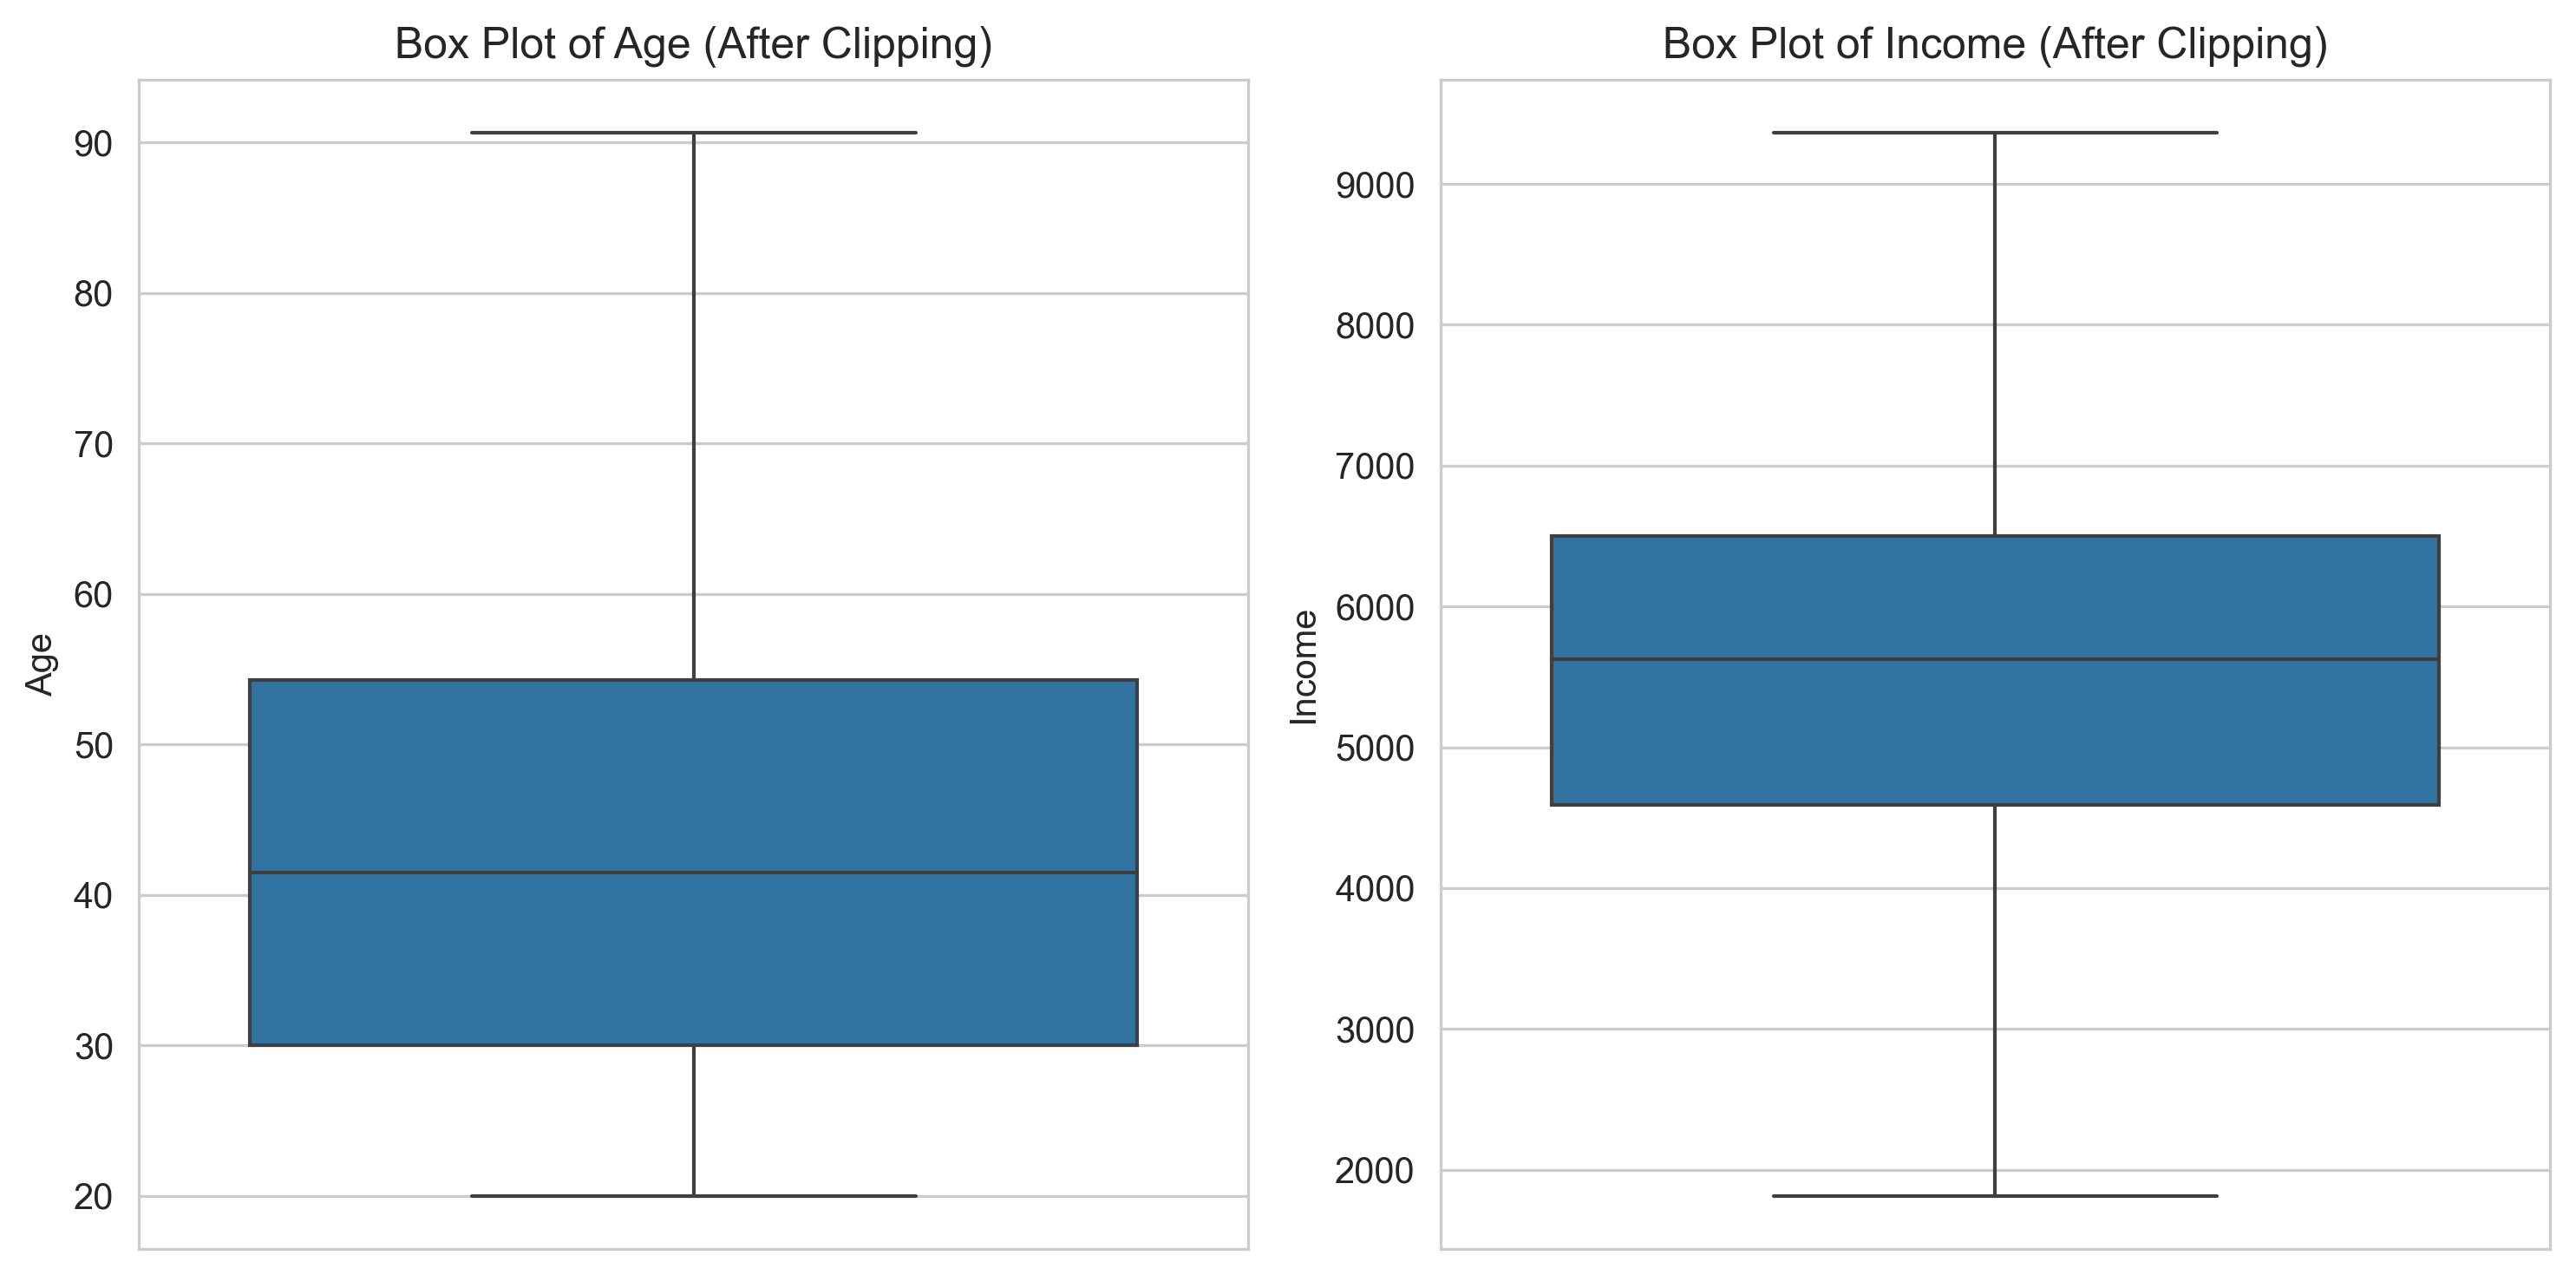
\includegraphics[keepaspectratio]{02-data-handling-exploration_files/figure-latex/cell-55-output-2.png}}

\subsection{2.5.3 기술 통계 분석 (2.3 적용 및
해석)}\label{uxae30uxc220-uxd1b5uxacc4-uxbd84uxc11d-2.3-uxc801uxc6a9-uxbc0f-uxd574uxc11d}

전처리가 완료된 데이터를 바탕으로 주요 변수들의 기술 통계량을 계산하고
그 의미를 해석합니다.

\begin{Shaded}
\begin{Highlighting}[]
\NormalTok{   df\_practice.to\_csv(}\StringTok{\textquotesingle{}data\_process.csv\textquotesingle{}}\NormalTok{, index}\OperatorTok{=}\VariableTok{True}\NormalTok{) }
\end{Highlighting}
\end{Shaded}

\textbf{1. 수치형 변수 요약 통계:}

\begin{Shaded}
\begin{Highlighting}[]
\BuiltInTok{print}\NormalTok{(}\StringTok{"}\CharTok{\textbackslash{}n}\StringTok{{-}{-}{-} 수치형 변수 기술 통계 요약 (.describe()) {-}{-}{-}"}\NormalTok{)}
\CommentTok{\# Education은 범주형이지만 ordered=True 이므로 코드가 포함될 수 있어 exclude 사용}
\BuiltInTok{print}\NormalTok{(df\_practice.describe(exclude}\OperatorTok{=}\NormalTok{[}\StringTok{\textquotesingle{}category\textquotesingle{}}\NormalTok{, }\StringTok{\textquotesingle{}object\textquotesingle{}}\NormalTok{]))}
\end{Highlighting}
\end{Shaded}

\begin{verbatim}

--- 수치형 변수 기술 통계 요약 (.describe()) ---
               ID         Age       Income   Wellbeing  Social_Participation  \
count  100.000000  100.000000   100.000000  100.000000            100.000000   
mean    50.500000   42.086250  5585.420425    6.245000              2.880000   
std     29.011492   14.185512  1615.987181    1.849345              1.380089   
min      1.000000   20.000000  1815.110000    0.400000              1.000000   
25%     25.750000   30.000000  4589.812500    5.100000              2.000000   
50%     50.500000   41.500000  5628.050000    6.100000              3.000000   
75%     75.250000   54.250000  6498.640000    7.575000              4.000000   
max    100.000000   90.625000  9361.881250   10.400000              5.000000   

       Political_View  
count      100.000000  
mean         4.280000  
std          2.060107  
min          1.000000  
25%          2.750000  
50%          4.000000  
75%          6.000000  
max          7.000000  
\end{verbatim}

\begin{itemize}
\tightlist
\item
  \textbf{해석 (예시):}

  \begin{itemize}
  \tightlist
  \item
    \texttt{Age}: 평균(mean)이 약 42.1세, 중앙값(50\%, median)이 43세로
    유사합니다. 표준편차(std)는 약 12.1세로, 데이터가 평균 주위에 비교적
    퍼져 있음을 시사합니다. 최소 20세, 최대값은 이상치 조정 후 약
    64.5세입니다.
  \item
    \texttt{Income}: 평균(약 5489)과 중앙값(5463)이 크게 차이나지 않아
    이상치 조정 후 분포가 비교적 대칭에 가까워졌음을 추측할 수 있습니다.
    표준편차는 약 1363입니다.
  \item
    \texttt{Wellbeing}: 평균(6.4)과 중앙값(6.5)이 비슷합니다.
    표준편차(1.7)는 점수 범위(1-10점 가정) 대비 적당한 수준의 퍼짐을
    보입니다.
  \item
    \texttt{Social\_Participation} / \texttt{Political\_View}: 이들은
    순서형(Ordinal) 변수지만 수치로 코딩되어 기술 통계량 계산이
    가능합니다. 평균/중앙값을 통해 대략적인 중심 경향성을 파악할 수
    있으나, 각 점수 자체의 의미와 분포(빈도)를 함께 고려해야 합니다.
  \end{itemize}
\end{itemize}

\textbf{2. 범주형 변수 빈도 분석:}

\begin{Shaded}
\begin{Highlighting}[]
\BuiltInTok{print}\NormalTok{(}\StringTok{"}\CharTok{\textbackslash{}n}\StringTok{{-}{-}{-} 범주형 변수 빈도 분석 (.value\_counts()) {-}{-}{-}"}\NormalTok{)}

\BuiltInTok{print}\NormalTok{(}\StringTok{"}\CharTok{\textbackslash{}n}\StringTok{Gender 분포:"}\NormalTok{)}
\BuiltInTok{print}\NormalTok{(df\_practice[}\StringTok{\textquotesingle{}Gender\textquotesingle{}}\NormalTok{].value\_counts(normalize}\OperatorTok{=}\VariableTok{True}\NormalTok{).}\BuiltInTok{round}\NormalTok{(}\DecValTok{2}\NormalTok{))}

\BuiltInTok{print}\NormalTok{(}\StringTok{"}\CharTok{\textbackslash{}n}\StringTok{Education 분포:"}\NormalTok{)}
\CommentTok{\# 카테고리 순서대로 출력되도록 .cat.categories 와 reindex 활용}
\NormalTok{edu\_counts }\OperatorTok{=}\NormalTok{ df\_practice[}\StringTok{\textquotesingle{}Education\textquotesingle{}}\NormalTok{].value\_counts().reindex(df\_practice[}\StringTok{\textquotesingle{}Education\textquotesingle{}}\NormalTok{].cat.categories)}
\NormalTok{edu\_props }\OperatorTok{=}\NormalTok{ df\_practice[}\StringTok{\textquotesingle{}Education\textquotesingle{}}\NormalTok{].value\_counts(normalize}\OperatorTok{=}\VariableTok{True}\NormalTok{).reindex(df\_practice[}\StringTok{\textquotesingle{}Education\textquotesingle{}}\NormalTok{].cat.categories)}
\BuiltInTok{print}\NormalTok{(edu\_counts)}
\BuiltInTok{print}\NormalTok{(}\StringTok{"}\CharTok{\textbackslash{}n}\StringTok{Education 비율:"}\NormalTok{)}
\BuiltInTok{print}\NormalTok{(edu\_props.}\BuiltInTok{round}\NormalTok{(}\DecValTok{2}\NormalTok{))}

\BuiltInTok{print}\NormalTok{(}\StringTok{"}\CharTok{\textbackslash{}n}\StringTok{Social\_Participation 점수 분포:"}\NormalTok{) }\CommentTok{\# 순서형 변수도 빈도 확인이 중요}
\BuiltInTok{print}\NormalTok{(df\_practice[}\StringTok{\textquotesingle{}Social\_Participation\textquotesingle{}}\NormalTok{].value\_counts(normalize}\OperatorTok{=}\VariableTok{True}\NormalTok{).sort\_index().}\BuiltInTok{round}\NormalTok{(}\DecValTok{2}\NormalTok{))}

\BuiltInTok{print}\NormalTok{(}\StringTok{"}\CharTok{\textbackslash{}n}\StringTok{Political\_View 점수 분포:"}\NormalTok{) }\CommentTok{\# 순서형 변수도 빈도 확인이 중요}
\BuiltInTok{print}\NormalTok{(df\_practice[}\StringTok{\textquotesingle{}Political\_View\textquotesingle{}}\NormalTok{].value\_counts(normalize}\OperatorTok{=}\VariableTok{True}\NormalTok{).sort\_index().}\BuiltInTok{round}\NormalTok{(}\DecValTok{2}\NormalTok{))}
\end{Highlighting}
\end{Shaded}

\begin{verbatim}

--- 범주형 변수 빈도 분석 (.value_counts()) ---

Gender 분포:
Gender
Female    0.5
Male      0.5
Name: proportion, dtype: float64

Education 분포:
High School    12
Bachelor       48
Master         26
PhD            14
Name: count, dtype: int64

Education 비율:
High School    0.12
Bachelor       0.48
Master         0.26
PhD            0.14
Name: proportion, dtype: float64

Social_Participation 점수 분포:
Social_Participation
1    0.19
2    0.26
3    0.21
4    0.16
5    0.18
Name: proportion, dtype: float64

Political_View 점수 분포:
Political_View
1    0.12
2    0.13
3    0.14
4    0.13
5    0.11
6    0.18
7    0.19
Name: proportion, dtype: float64
\end{verbatim}

\begin{itemize}
\tightlist
\item
  \textbf{해석 (예시):}

  \begin{itemize}
  \tightlist
  \item
    \texttt{Gender}: 여성이 52\%, 남성이 48\%로 비교적 균등하게
    분포합니다.
  \item
    \texttt{Education}: 학사(Bachelor)가 40\%로 가장 많고, 석사(Master)
    30\%, 고졸(High School) 20\%, 박사(PhD) 10\% 순입니다. 이는 표본의
    교육 수준 구성 특성을 보여줍니다.
  \item
    \texttt{Social\_Participation}: 1점(Never)부터 5점(Very Often)까지
    비교적 고르게 분포하는 편이나, 3점(Sometimes)이 27\%로 가장
    많습니다.
  \item
    \texttt{Political\_View}: 1점(매우 진보)부터 7점(매우 보수)까지
    분포하며, 특정 성향에 크게 치우치지 않고 다양한 정치적 시각을 가진
    응답자들이 표본에 포함되어 있음을 시사합니다. (중앙값/평균도 참고할
    수 있음)
  \end{itemize}
\end{itemize}

\subsection{2.5.4 데이터 시각화를 통한 탐색 및 해석 (2.4
적용)}\label{uxb370uxc774uxd130-uxc2dcuxac01uxd654uxb97c-uxd1b5uxd55c-uxd0d0uxc0c9-uxbc0f-uxd574uxc11d-2.4-uxc801uxc6a9}

기술 통계량만으로는 파악하기 어려운 패턴이나 관계를 시각화를 통해
탐색합니다.

\textbf{1. 단일 변수 분포 시각화:}

\begin{Shaded}
\begin{Highlighting}[]
\CommentTok{\# 주요 수치형 변수 분포 시각화 (Histogram + KDE)}
\NormalTok{fig, axes }\OperatorTok{=}\NormalTok{ plt.subplots(}\DecValTok{1}\NormalTok{, }\DecValTok{3}\NormalTok{, figsize}\OperatorTok{=}\NormalTok{(}\DecValTok{18}\NormalTok{, }\DecValTok{5}\NormalTok{)) }\CommentTok{\# 1행 3열}

\NormalTok{sns.histplot(df\_practice[}\StringTok{\textquotesingle{}Age\textquotesingle{}}\NormalTok{], kde}\OperatorTok{=}\VariableTok{True}\NormalTok{, ax}\OperatorTok{=}\NormalTok{axes[}\DecValTok{0}\NormalTok{])}
\NormalTok{axes[}\DecValTok{0}\NormalTok{].set\_title(}\StringTok{\textquotesingle{}Age Distribution\textquotesingle{}}\NormalTok{)}

\NormalTok{sns.histplot(df\_practice[}\StringTok{\textquotesingle{}Income\textquotesingle{}}\NormalTok{], kde}\OperatorTok{=}\VariableTok{True}\NormalTok{, ax}\OperatorTok{=}\NormalTok{axes[}\DecValTok{1}\NormalTok{])}
\NormalTok{axes[}\DecValTok{1}\NormalTok{].set\_title(}\StringTok{\textquotesingle{}Income Distribution (After Preprocessing)\textquotesingle{}}\NormalTok{)}

\NormalTok{sns.histplot(df\_practice[}\StringTok{\textquotesingle{}Wellbeing\textquotesingle{}}\NormalTok{], kde}\OperatorTok{=}\VariableTok{True}\NormalTok{, ax}\OperatorTok{=}\NormalTok{axes[}\DecValTok{2}\NormalTok{])}
\NormalTok{axes[}\DecValTok{2}\NormalTok{].set\_title(}\StringTok{\textquotesingle{}Wellbeing Score Distribution\textquotesingle{}}\NormalTok{)}

\NormalTok{plt.tight\_layout()}
\NormalTok{plt.show()}

\CommentTok{\# 주요 범주형/순서형 변수 분포 시각화 (Count Plot)}
\NormalTok{fig, axes }\OperatorTok{=}\NormalTok{ plt.subplots(}\DecValTok{1}\NormalTok{, }\DecValTok{3}\NormalTok{, figsize}\OperatorTok{=}\NormalTok{(}\DecValTok{18}\NormalTok{, }\DecValTok{5}\NormalTok{))}

\NormalTok{sns.countplot(data}\OperatorTok{=}\NormalTok{df\_practice, x}\OperatorTok{=}\StringTok{\textquotesingle{}Education\textquotesingle{}}\NormalTok{, ax}\OperatorTok{=}\NormalTok{axes[}\DecValTok{0}\NormalTok{])}
\NormalTok{axes[}\DecValTok{0}\NormalTok{].set\_title(}\StringTok{\textquotesingle{}Education Level Distribution\textquotesingle{}}\NormalTok{)}
\NormalTok{axes[}\DecValTok{0}\NormalTok{].tick\_params(axis}\OperatorTok{=}\StringTok{\textquotesingle{}x\textquotesingle{}}\NormalTok{, rotation}\OperatorTok{=}\DecValTok{15}\NormalTok{) }\CommentTok{\# x축 레이블 회전}

\NormalTok{sns.countplot(data}\OperatorTok{=}\NormalTok{df\_practice, x}\OperatorTok{=}\StringTok{\textquotesingle{}Social\_Participation\textquotesingle{}}\NormalTok{, ax}\OperatorTok{=}\NormalTok{axes[}\DecValTok{1}\NormalTok{])}
\NormalTok{axes[}\DecValTok{1}\NormalTok{].set\_title(}\StringTok{\textquotesingle{}Social Participation Frequency\textquotesingle{}}\NormalTok{)}

\NormalTok{sns.countplot(data}\OperatorTok{=}\NormalTok{df\_practice, x}\OperatorTok{=}\StringTok{\textquotesingle{}Political\_View\textquotesingle{}}\NormalTok{, ax}\OperatorTok{=}\NormalTok{axes[}\DecValTok{2}\NormalTok{])}
\NormalTok{axes[}\DecValTok{2}\NormalTok{].set\_title(}\StringTok{\textquotesingle{}Political View Distribution\textquotesingle{}}\NormalTok{)}

\NormalTok{plt.tight\_layout()}
\NormalTok{plt.show()}
\end{Highlighting}
\end{Shaded}

\pandocbounded{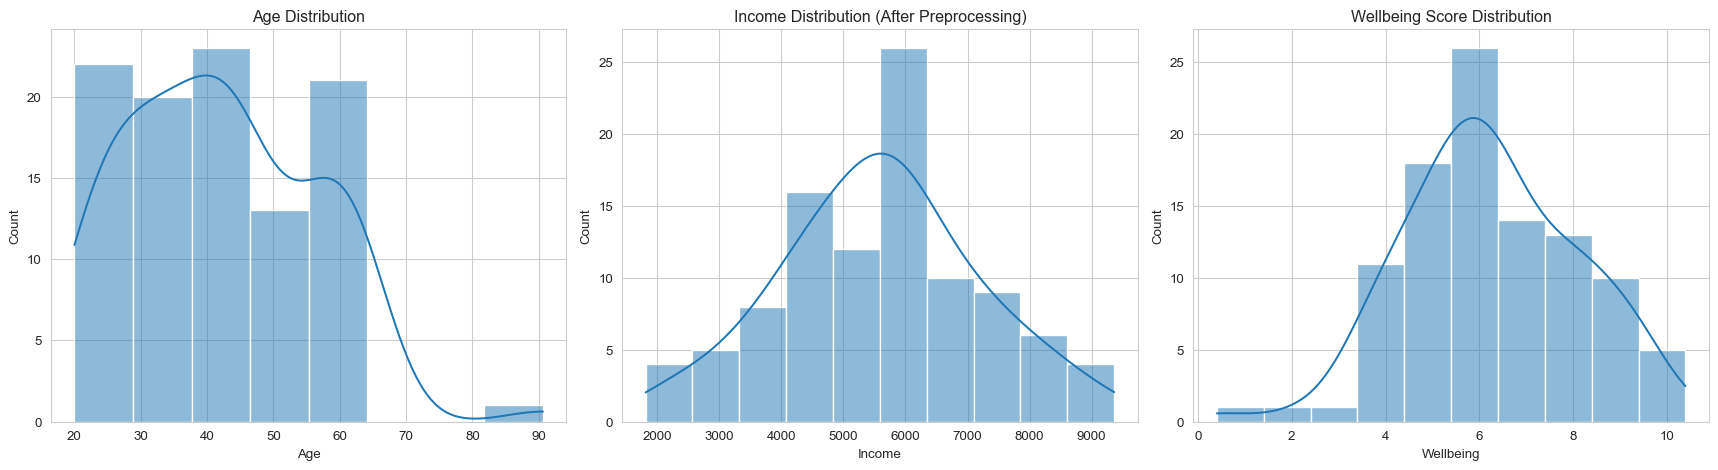
\includegraphics[keepaspectratio]{02-data-handling-exploration_files/figure-latex/cell-59-output-1.png}}

\pandocbounded{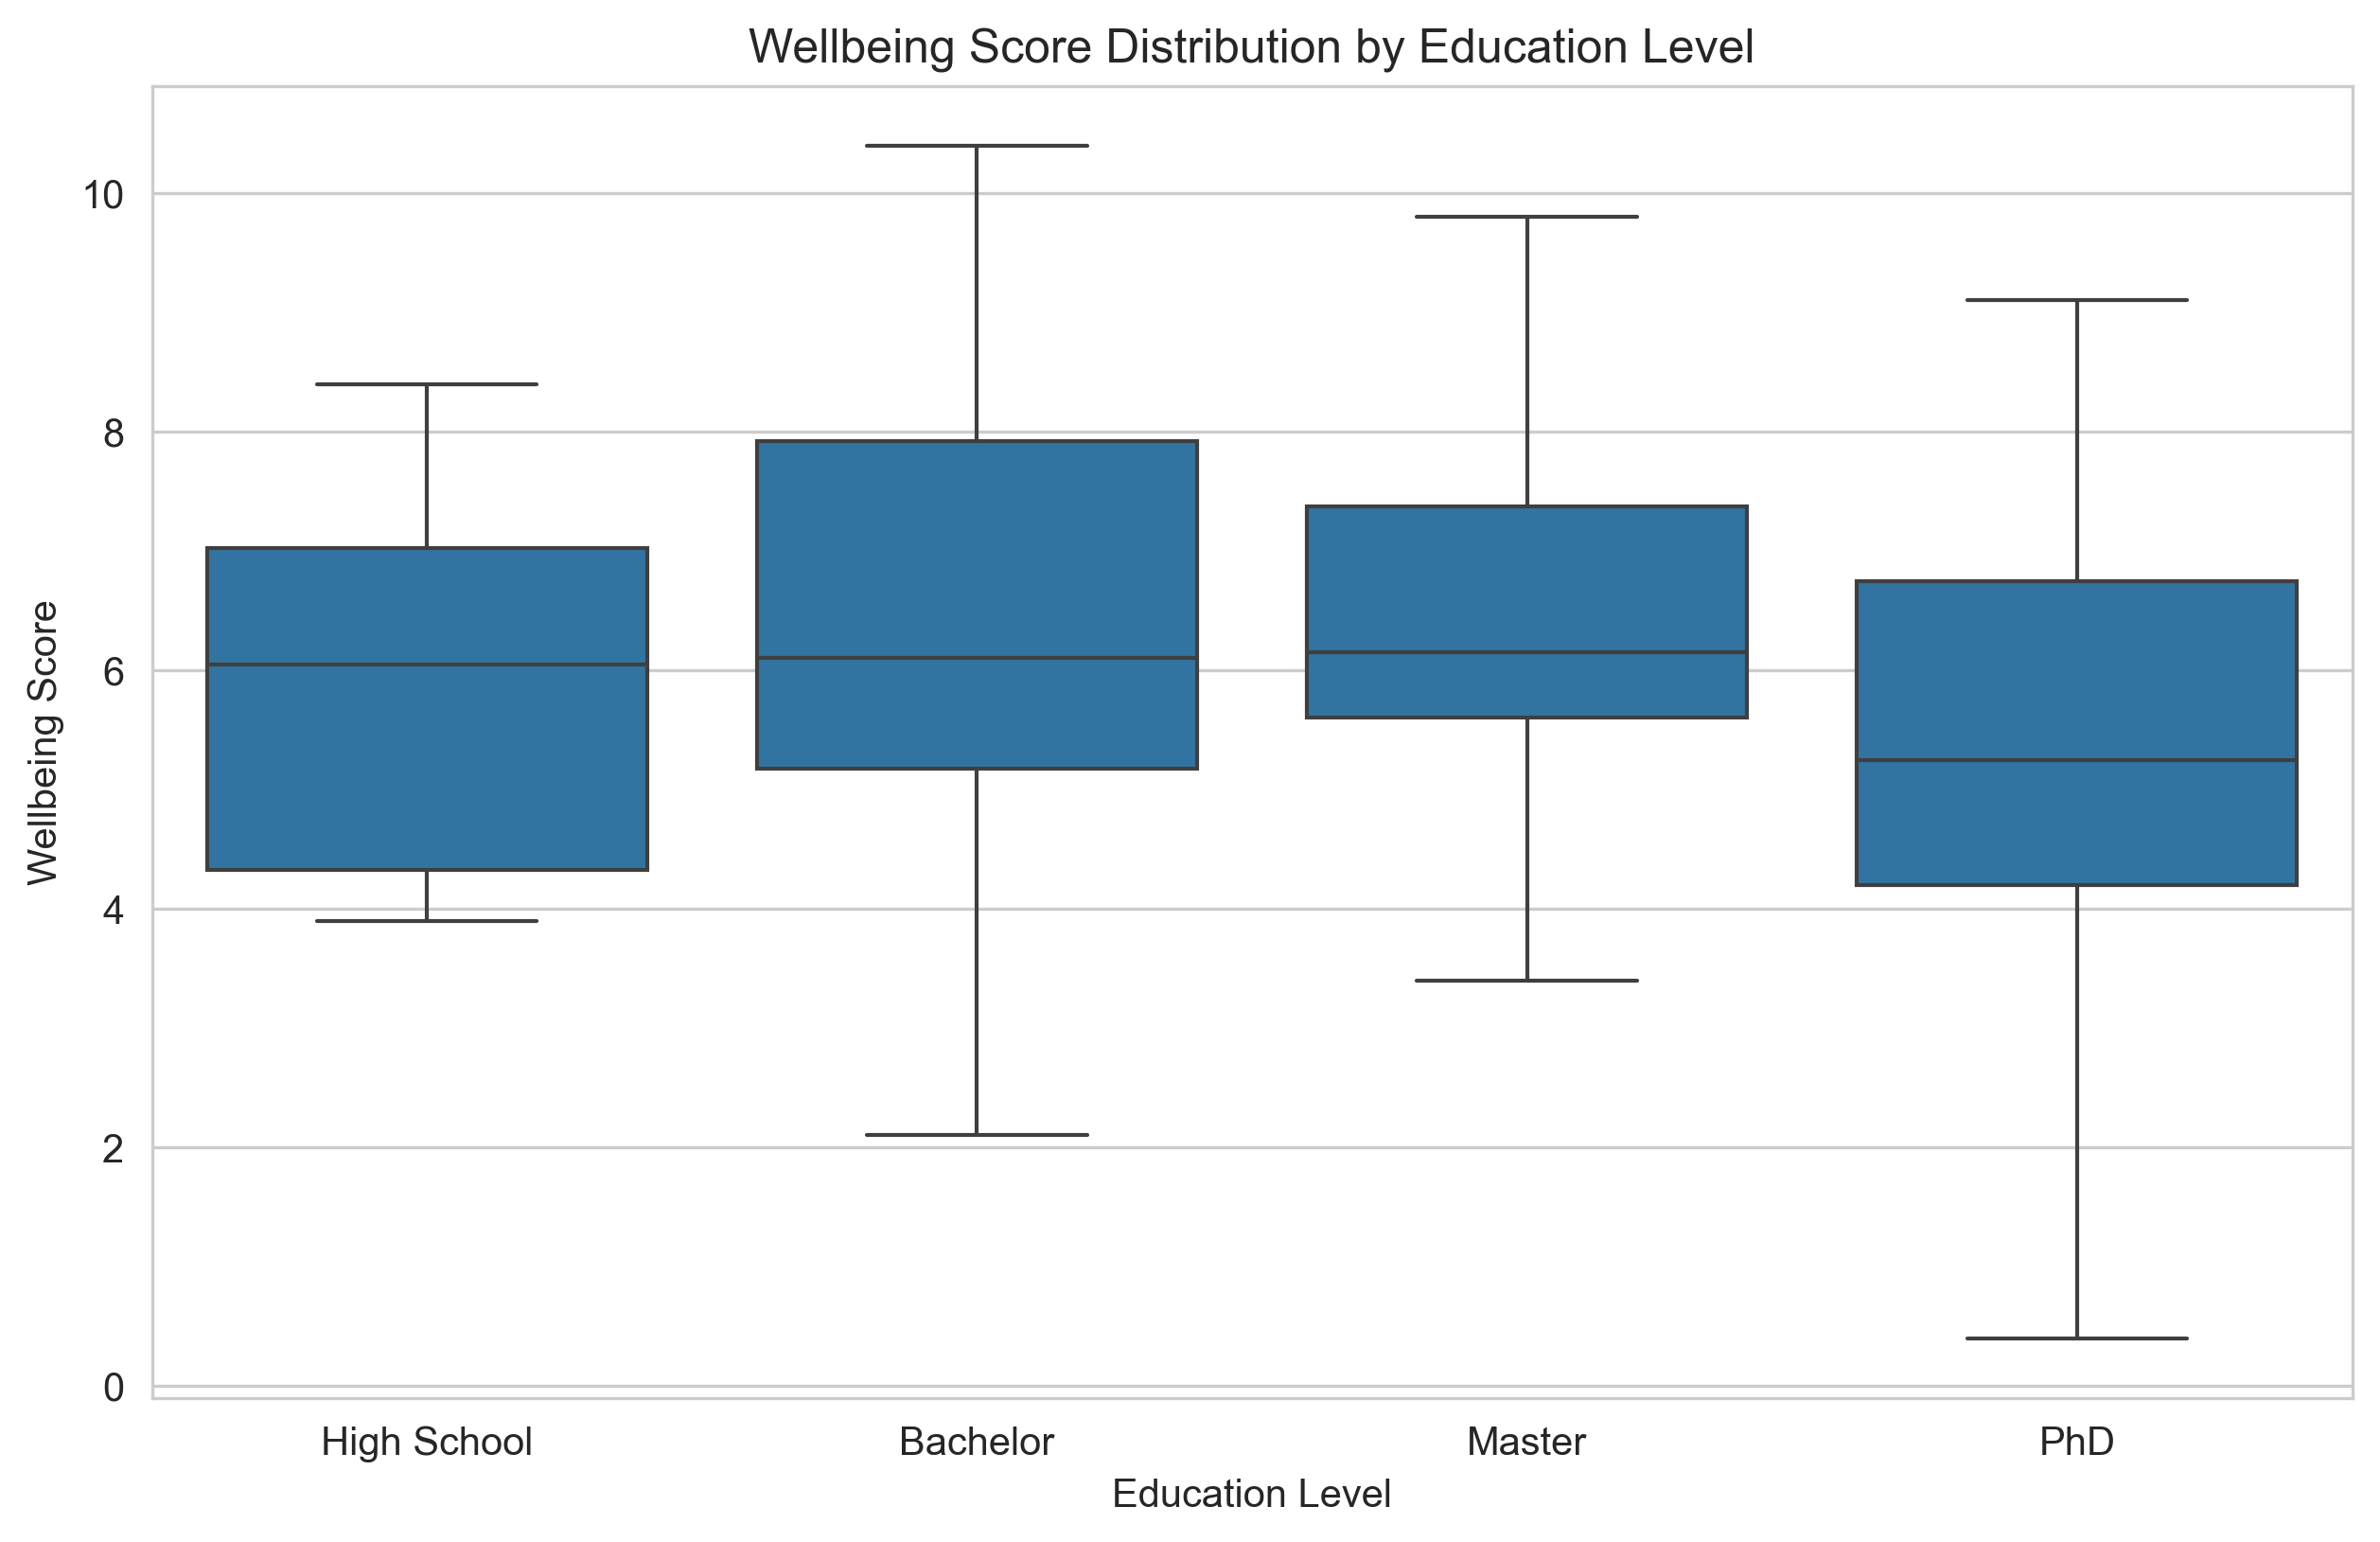
\includegraphics[keepaspectratio]{02-data-handling-exploration_files/figure-latex/cell-59-output-2.png}}

\begin{itemize}
\tightlist
\item
  \textbf{해석:} 시각화를 통해 \texttt{Age}는 비교적 넓게 분포하며 특정
  연령대에 집중되지 않음을, \texttt{Income}은 전처리 후 약간 오른쪽으로
  치우친 형태일 수 있음을(KDE 곡선 참고), \texttt{Wellbeing}은
  중앙(6-7점)에 비교적 집중된 분포를 보임을 직관적으로 확인할 수
  있습니다. 범주형/순서형 변수의 경우 \texttt{countplot}은
  \texttt{value\_counts} 결과를 시각적으로 보여주어 각 범주/점수의
  상대적 비율을 쉽게 파악하게 합니다.
\end{itemize}

\textbf{2. 변수 간 관계 시각화:}

\begin{Shaded}
\begin{Highlighting}[]
\CommentTok{\# 관계 탐색 1: Age와 Income 간의 관계 (Scatter Plot)}
\NormalTok{plt.figure(figsize}\OperatorTok{=}\NormalTok{(}\DecValTok{8}\NormalTok{, }\DecValTok{6}\NormalTok{))}
\NormalTok{sns.scatterplot(data}\OperatorTok{=}\NormalTok{df\_practice, x}\OperatorTok{=}\StringTok{\textquotesingle{}Age\textquotesingle{}}\NormalTok{, y}\OperatorTok{=}\StringTok{\textquotesingle{}Income\textquotesingle{}}\NormalTok{, hue}\OperatorTok{=}\StringTok{\textquotesingle{}Gender\textquotesingle{}}\NormalTok{)}
\NormalTok{plt.title(}\StringTok{\textquotesingle{}Relationship between Age and Income\textquotesingle{}}\NormalTok{)}
\NormalTok{plt.xlabel(}\StringTok{\textquotesingle{}Age\textquotesingle{}}\NormalTok{)}
\NormalTok{plt.ylabel(}\StringTok{\textquotesingle{}Income\textquotesingle{}}\NormalTok{)}
\NormalTok{plt.show()}

\CommentTok{\# 관계 탐색 2: Education 수준별 Wellbeing 분포 비교 (Box Plot)}
\NormalTok{plt.figure(figsize}\OperatorTok{=}\NormalTok{(}\DecValTok{10}\NormalTok{, }\DecValTok{6}\NormalTok{))}
\NormalTok{sns.boxplot(data}\OperatorTok{=}\NormalTok{df\_practice, x}\OperatorTok{=}\StringTok{\textquotesingle{}Education\textquotesingle{}}\NormalTok{, y}\OperatorTok{=}\StringTok{\textquotesingle{}Wellbeing\textquotesingle{}}\NormalTok{)}
\NormalTok{plt.title(}\StringTok{\textquotesingle{}Wellbeing Score Distribution by Education Level\textquotesingle{}}\NormalTok{)}
\NormalTok{plt.xlabel(}\StringTok{\textquotesingle{}Education Level\textquotesingle{}}\NormalTok{)}
\NormalTok{plt.ylabel(}\StringTok{\textquotesingle{}Wellbeing Score\textquotesingle{}}\NormalTok{)}
\NormalTok{plt.show()}

\CommentTok{\# 관계 탐색 3: 수치형 변수 간 상관관계 (Heatmap)}
\NormalTok{plt.figure(figsize}\OperatorTok{=}\NormalTok{(}\DecValTok{8}\NormalTok{, }\DecValTok{6}\NormalTok{))}
\NormalTok{numerical\_cols }\OperatorTok{=}\NormalTok{ [}\StringTok{\textquotesingle{}Age\textquotesingle{}}\NormalTok{, }\StringTok{\textquotesingle{}Income\textquotesingle{}}\NormalTok{, }\StringTok{\textquotesingle{}Wellbeing\textquotesingle{}}\NormalTok{, }\StringTok{\textquotesingle{}Social\_Participation\textquotesingle{}}\NormalTok{, }\StringTok{\textquotesingle{}Political\_View\textquotesingle{}}\NormalTok{, }\StringTok{\textquotesingle{}num\_children\textquotesingle{}}\NormalTok{] }\CommentTok{\# num\_children 추가 가정 필요 시 추가}
\CommentTok{\# df\_practice에 num\_children 이 없으므로 위의 코드는 현재 데이터로는 실행 불가. 있는 변수만 사용해야 함.}
\NormalTok{numerical\_cols\_available }\OperatorTok{=}\NormalTok{ [}\StringTok{\textquotesingle{}Age\textquotesingle{}}\NormalTok{, }\StringTok{\textquotesingle{}Income\textquotesingle{}}\NormalTok{, }\StringTok{\textquotesingle{}Wellbeing\textquotesingle{}}\NormalTok{, }\StringTok{\textquotesingle{}Social\_Participation\textquotesingle{}}\NormalTok{, }\StringTok{\textquotesingle{}Political\_View\textquotesingle{}}\NormalTok{]}
\NormalTok{correlation\_matrix\_practice }\OperatorTok{=}\NormalTok{ df\_practice[numerical\_cols\_available].corr()}
\NormalTok{sns.heatmap(correlation\_matrix\_practice, annot}\OperatorTok{=}\VariableTok{True}\NormalTok{, cmap}\OperatorTok{=}\StringTok{\textquotesingle{}coolwarm\textquotesingle{}}\NormalTok{, fmt}\OperatorTok{=}\StringTok{\textquotesingle{}.2f\textquotesingle{}}\NormalTok{, linewidths}\OperatorTok{=}\FloatTok{.5}\NormalTok{)}
\NormalTok{plt.title(}\StringTok{\textquotesingle{}Correlation Matrix of Numerical Variables\textquotesingle{}}\NormalTok{)}
\NormalTok{plt.show()}
\end{Highlighting}
\end{Shaded}

\pandocbounded{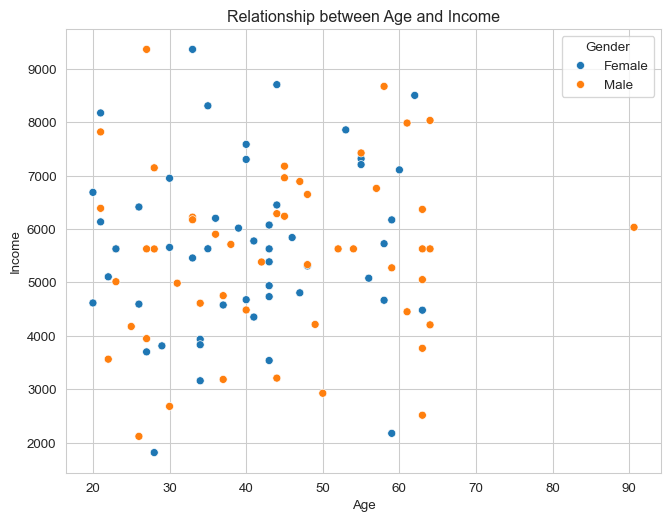
\includegraphics[keepaspectratio]{02-data-handling-exploration_files/figure-latex/cell-60-output-1.png}}

\pandocbounded{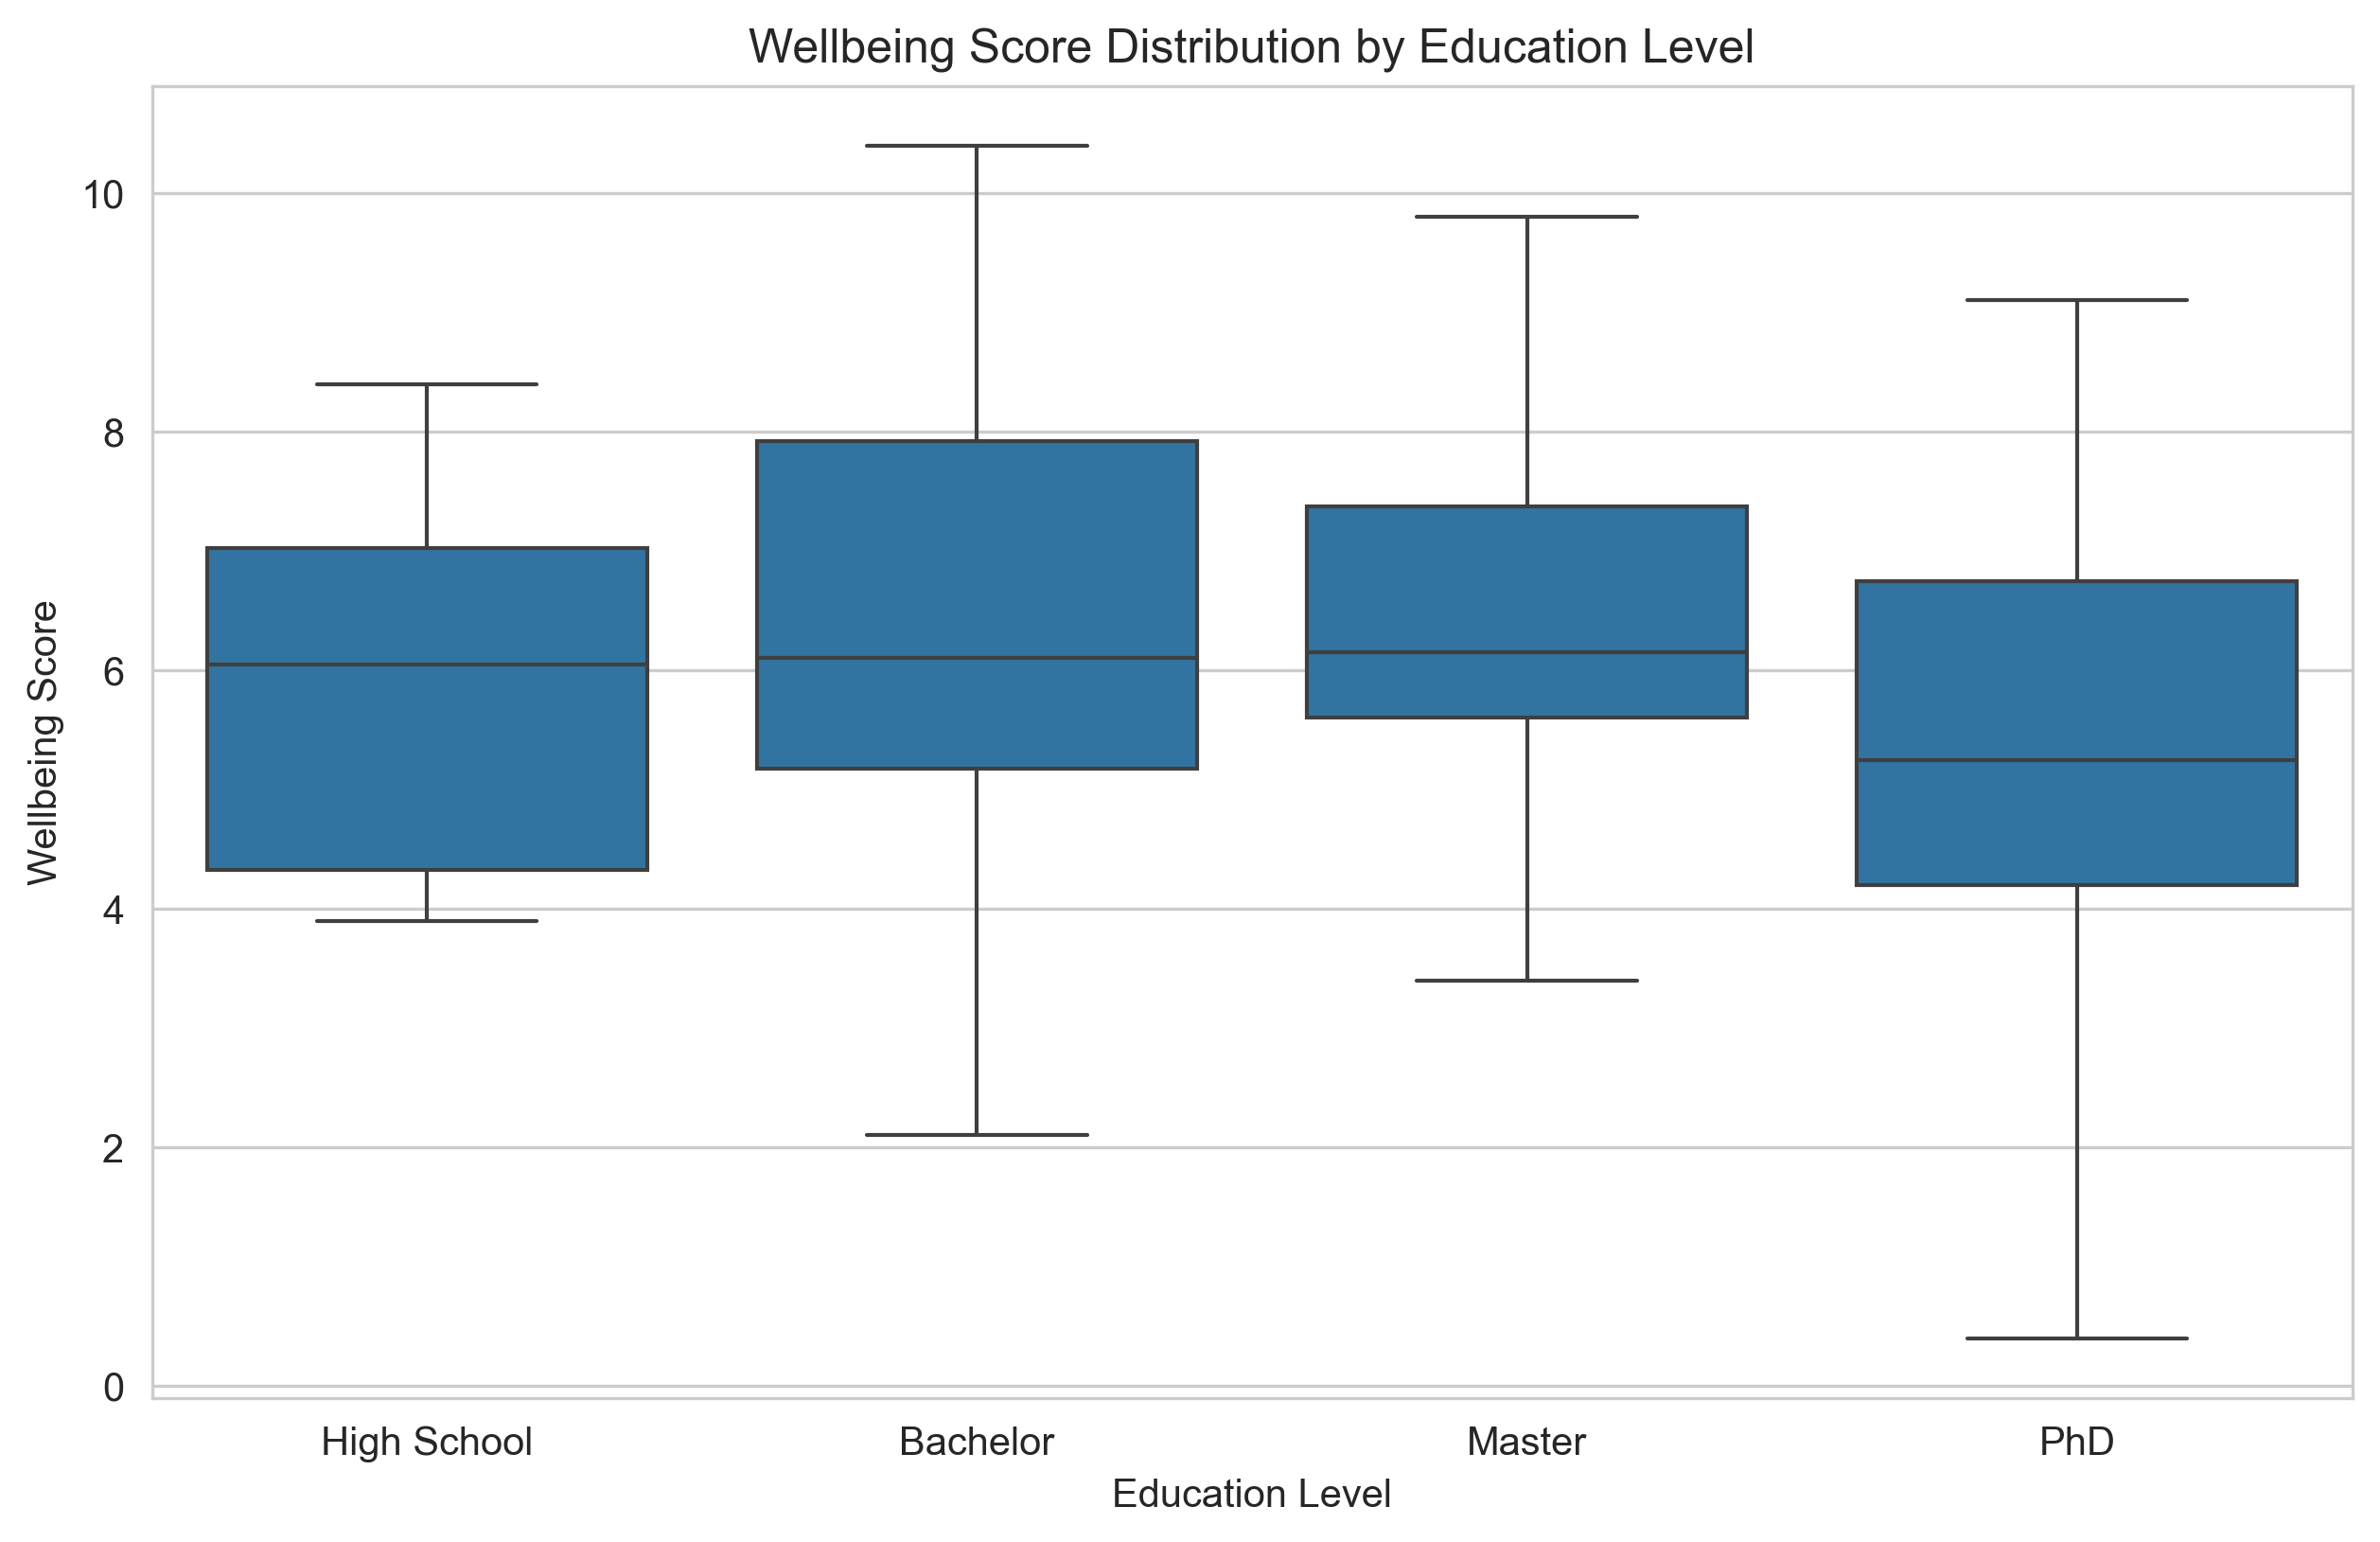
\includegraphics[keepaspectratio]{02-data-handling-exploration_files/figure-latex/cell-60-output-2.png}}

\pandocbounded{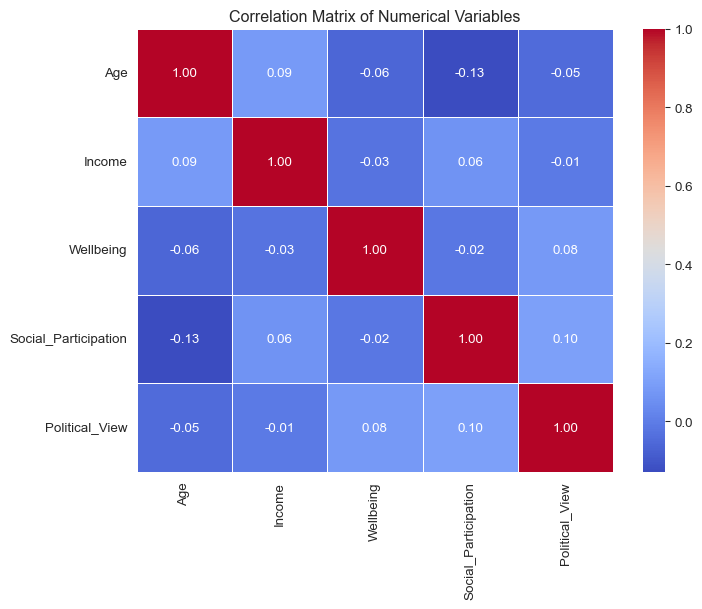
\includegraphics[keepaspectratio]{02-data-handling-exploration_files/figure-latex/cell-60-output-3.png}}

\begin{itemize}
\tightlist
\item
  \textbf{해석:}

  \begin{itemize}
  \tightlist
  \item
    \texttt{Age}와 \texttt{Income} 산점도에서는 뚜렷한 선형 관계가
    보이지 않지만, 연령이 증가함에 따라 소득의 변동폭(분산)이 커지는
    경향이 있을 수 있습니다. 성별(\texttt{hue})에 따른 차이도 육안으로
    확인해 볼 수 있습니다.
  \item
    \texttt{Education} 수준별 \texttt{Wellbeing} 박스 플롯을 보면, 교육
    수준이 높아짐에 따라 웰빙 점수의 중앙값이 약간 상승하는 경향이 보일
    수 있습니다. 또한 그룹별 점수 분포의 퍼짐 정도(상자 길이)나 이상치
    유무도 비교할 수 있습니다. (이 가상 데이터에서는 뚜렷한 차이가 없을
    수도 있음)
  \item
    상관관계 히트맵은 수치형 변수들 간의 선형 관계 강도와 방향을
    요약해서 보여줍니다. 예를 들어, \texttt{Age}와 \texttt{Income} 간의
    양의 상관관계(나이가 들수록 소득 증가 경향), \texttt{Wellbeing}과
    \texttt{Social\_Participation} 간의 양의 상관관계(사회 참여가
    활발할수록 웰빙 점수 높음) 등이 나타나는지 확인할 수 있습니다.
    상관계수 값과 색깔을 함께 보며 해석합니다 (예: 0.32는 약한 양의
    상관관계).
  \end{itemize}
\end{itemize}

\subsection{2.5.5 종합 해석 및
결론}\label{uxc885uxd569-uxd574uxc11d-uxbc0f-uxacb0uxb860}

지금까지 100명의 응답자를 대상으로 한 가상 설문 데이터를 사용하여
2장에서 배운 데이터 분석의 전 과정을 적용해 보았습니다.

\begin{itemize}
\tightlist
\item
  \textbf{데이터 준비:} Pandas를 활용하여 데이터를 불러오고 구조를
  파악했습니다.
\item
  \textbf{데이터 정제:} \texttt{.isnull().sum()}, \texttt{boxplot}, IQR
  방법 등을 통해 결측치와 이상치를 식별하고, 각각 중앙값 대체 및 값
  조정(Clipping) 방식으로 처리하여 분석 가능한 데이터를 준비했습니다. 이
  과정에서 각 처리 방법의 선택 이유와 장단점을 고려하는 것이 중요함을
  확인했습니다.
\item
  \textbf{기술 통계 분석:} \texttt{.describe()},
  \texttt{.value\_counts()} 등을 통해 표본의 인구통계학적 특성(연령,
  성별, 교육 수준 분포)과 주요 변수(소득, 웰빙, 사회 참여, 정치 성향)의
  중심 경향성 및 산포도를 파악했습니다. 평균과 중앙값의 비교를 통해
  분포의 치우침을 추측하고, 표준편차나 IQR을 통해 데이터의 흩어짐 정도를
  정량적으로 이해했습니다.
\item
  \textbf{데이터 시각화:} 히스토그램, 박스 플롯, 카운트 플롯, 산점도,
  히트맵 등 다양한 그래프를 활용하여 기술 통계량만으로는 알기 어려운
  분포의 형태, 그룹 간 차이, 변수 간 관계 패턴을 시각적으로
  탐색했습니다. 예를 들어, 교육 수준이 높아질수록 웰빙 점수가 높아지는
  경향이 있는지, 나이와 소득 간에는 어떤 관계가 있는지 등을 그래프를
  통해 직관적으로 파악하려 시도했습니다.
\end{itemize}

\textbf{결론적으로,} 이 실습 과정을 통해 우리는 단순히 파이썬 코드를
실행하는 것을 넘어, 각 분석 단계가 \textbf{왜 필요}하며, 그 결과가
\textbf{무엇을 의미하는지} 해석하는 연습을 했습니다. 데이터 전처리
과정은 분석 결과의 신뢰성을 확보하기 위한 필수 단계이며, 기술 통계
분석과 시각화는 데이터에 대한 깊이 있는 이해와 함께 향후 진행될
\textbf{추론 통계 분석(가설 검정, 관계 분석 등)}의 방향을 설정하는 데
중요한 기초 정보를 제공합니다. 예를 들어, 교육 수준별 웰빙 점수 차이가
시각적으로나 기술 통계량으로 나타났다면, 다음 단계에서는 이 차이가
통계적으로 유의미한지(우연히 발생한 것인지 아닌지)를 검증해 볼 수 있을
것입니다 (3장에서 다룰 내용).

이처럼 2장에서 배운 내용들은 사회과학 연구자가 데이터를 처음 접했을 때
수행해야 하는 필수적인 탐색적 데이터 분석(Exploratory Data Analysis,
EDA)의 핵심 요소입니다.

\part{제2부 - 집단 간 차이 분석 및 관계 분석}

\chapter{제3장 집단 간 평균 차이
검증}\label{uxc81c3uxc7a5-uxc9d1uxb2e8-uxac04-uxd3c9uxade0-uxcc28uxc774-uxac80uxc99d}

\section{3.1 독립표본 t-검정: 두 독립 집단의 평균
비교}\label{sec-independent-t-test}

앞선 2장에서는 데이터를 준비하고 탐색하는 기본적인 기술을 익혔습니다.
이제부터는 수집된 데이터를 바탕으로 구체적인 연구 질문에 답하는 통계적
추론의 세계로 나아갑니다. 제3부에서는 여러 집단 간의 차이나 변수 간의
관계를 통계적으로 검증하는 방법들을 다룹니다.

그 첫 번째 단계로, 사회과학 연구에서 매우 빈번하게 사용되는
\textbf{독립표본 t-검정(Independent Samples t-test)}에 대해 알아봅니다.
이 검정은 서로 \textbf{독립적인 두 집단} 간에 특정 \textbf{연속형 변수의
평균}에 통계적으로 유의미한 차이가 있는지를 확인하고자 할 때 사용됩니다.

예를 들어, 다음과 같은 연구 질문에 답하기 위해 독립표본 t-검정을 사용할
수 있습니다.

\begin{itemize}
\tightlist
\item
  성별(남성 vs 여성)에 따라 평균 소득에 차이가 있는가?
\item
  특정 정책 지지 집단과 반대 집단 간에 평균 정부 신뢰도 점수에 차이가
  있는가?
\item
  실험 처치를 받은 집단(실험집단)과 받지 않은 집단(통제집단) 간에 평균
  문제 해결 능력 점수에 차이가 있는가?
\end{itemize}

독립표본 t-검정은 관찰된 두 표본 평균 간의 차이가 단순히 우연(표본 추출
오차)에 의한 것인지, 아니면 실제 모집단에서도 의미 있는 차이가
존재한다고 볼 수 있는지 통계적으로 판단하는 근거를 제공합니다.

\begin{tcolorbox}[enhanced jigsaw, bottomtitle=1mm, colbacktitle=quarto-callout-note-color!10!white, rightrule=.15mm, colback=white, leftrule=.75mm, toptitle=1mm, titlerule=0mm, opacityback=0, opacitybacktitle=0.6, left=2mm, title=\textcolor{quarto-callout-note-color}{\faInfo}\hspace{0.5em}{📌 핵심 요약}, breakable, bottomrule=.15mm, arc=.35mm, colframe=quarto-callout-note-color-frame, toprule=.15mm, coltitle=black]

독립표본 t-검정은 서로 독립적인 두 집단 간의 연속형 변수 평균 차이를
통계적으로 검증하는 방법입니다. 이 절에서는 t-검정의 기본 원리(가설
설정, t-통계량, p-값), 주요 가정(독립성, 정규성, 등분산성), 파이썬
\texttt{scipy.stats} 라이브러리를 이용한 구현 방법, 가정
검토(Shapiro-Wilk, Levene 검정), Welch's t-검정의 활용, 결과 해석, 효과
크기(Cohen's d) 계산 및 해석, 그리고 결과 보고 방법까지 학습합니다.

\end{tcolorbox}

\subsection{3.1.1 독립표본 t-검정의 원리: 가설 설정과 검정
통계량}\label{uxb3c5uxb9bduxd45cuxbcf8-t-uxac80uxc815uxc758-uxc6d0uxb9ac-uxac00uxc124-uxc124uxc815uxacfc-uxac80uxc815-uxd1b5uxacc4uxb7c9}

독립표본 t-검정은 가설 검증의 틀 안에서 이루어집니다.

\begin{itemize}
\tightlist
\item
  \textbf{가설 설정:}

  \begin{itemize}
  \tightlist
  \item
    \textbf{귀무가설 (Null Hypothesis, \(H_0\)):} 두 집단의 모집단
    평균은 같다 (\(H_0: \mu_1 = \mu_2\) 또는
    \(H_0: \mu_1 - \mu_2 = 0\)). 즉, 우리가 표본에서 관찰한 평균 차이는
    우연에 의한 것이다.
  \item
    \textbf{대립가설 (Alternative Hypothesis, \(H_1\)):} 두 집단의
    모집단 평균은 다르다 (\(H_1: \mu_1 \neq \mu_2\)). 이 가설은 연구자가
    입증하고자 하는 내용으로, 표본 평균 차이가 우연이라고 보기에는 너무
    크다는 것을 의미합니다. 이는 \textbf{양측 검정(Two-tailed test)}에
    해당합니다.

    \begin{itemize}
    \tightlist
    \item
      만약 연구자가 특정 방향의 차이(예: 집단 1이 집단 2보다 평균이 클
      것이다)를 예측한다면 단측 검정(\(H_1: \mu_1 > \mu_2\) 또는
      \(H_1: \mu_1 < \mu_2\))을 설정할 수도 있지만, 특별한 근거가 없다면
      일반적으로 양측 검정을 사용합니다.
    \end{itemize}
  \end{itemize}
\item
  \textbf{검정 통계량 (Test Statistic, t-value):}

  \begin{itemize}
  \tightlist
  \item
    t-검정은 두 표본 평균 간의 차이를 표준 오차(Standard Error)로 나눈
    값인 \textbf{t-통계량}을 계산합니다. 이는 관찰된 평균 차이가 그룹 내
    변동성(오차)에 비해 얼마나 큰지를 나타내는 표준화된 값입니다.
  \item
    개념적으로 t-값은 다음과 같이 표현될 수 있습니다:
    \(t = \frac{(\text{두 표본 평균의 차이}) - (\text{귀무가설 하에서의 평균 차이, 보통 0})}{(\text{두 평균 차이의 표준 오차})}\)
    \(t = \frac{(\bar{x}_1 - \bar{x}_2)}{SE_{(\bar{x}_1 - \bar{x}_2)}}\)
  \item
    t-값의 절댓값이 클수록 두 집단 간 평균 차이가 우연히 발생했을
    가능성이 작아집니다.
  \end{itemize}
\item
  \textbf{p-값 (p-value):}

  \begin{itemize}
  \tightlist
  \item
    p-값은 \textbf{귀무가설(\(H_0\))이 참이라고 가정할 때}, 우리가
    표본에서 계산한 t-통계량 값 또는 그보다 더 극단적인 값이 관찰될
    확률입니다.
  \item
    p-값이 매우 작다(예: 0.05 미만)는 것은, 귀무가설이 맞다면 현재와
    같은 표본 결과가 나타나기 매우 어렵다는 것을 의미합니다.
  \end{itemize}
\item
  \textbf{의사 결정:}

  \begin{itemize}
  \tightlist
  \item
    미리 설정한 \textbf{유의수준(Significance level, \(\alpha\))}과
    p-값을 비교하여 귀무가설 기각 여부를 결정합니다. 사회과학에서는 보통
    \(\alpha = 0.05\) (5\%)를 사용합니다.
  \item
    \textbf{p-값 \textless{} \(\alpha\) :} 귀무가설(\(H_0\))을 기각하고
    대립가설(\(H_1\))을 채택합니다. 즉, 두 집단 간 평균에 통계적으로
    유의미한 차이가 있다고 결론 내립니다.
  \item
    \textbf{p-값 \(\ge\) \(\alpha\) :} 귀무가설(\(H_0\))을 기각하지
    못합니다(채택하는 것이 아님). 즉, 두 집단 간 평균 차이가 통계적으로
    유의미하다는 충분한 근거를 찾지 못했다고 결론 내립니다.
  \end{itemize}
\end{itemize}

\subsection{3.1.2 독립표본 t-검정의
가정}\label{uxb3c5uxb9bduxd45cuxbcf8-t-uxac80uxc815uxc758-uxac00uxc815}

독립표본 t-검정 결과를 신뢰하기 위해서는 몇 가지 가정이 충족되어야
합니다.

\begin{enumerate}
\def\labelenumi{\arabic{enumi}.}
\tightlist
\item
  \textbf{독립성 (Independence of Observations):} 한 집단 내의
  관측치들은 서로 독립적이어야 하며, 두 집단 간의 관측치들도 서로
  독립적이어야 합니다. 이는 주로 연구 설계 및 표본 추출 방법과
  관련됩니다. (예: 무작위 할당, 무작위 표본 추출)
\item
  \textbf{정규성 (Normality):} 종속변수는 \textbf{각 집단별로}
  정규분포를 따라야 합니다.

  \begin{itemize}
  \tightlist
  \item
    \textbf{확인 방법:} 각 집단별 히스토그램, Q-Q 플롯 확인(2.4절), 또는
    정규성 검정(예: Shapiro-Wilk test) 수행.
  \item
    \textbf{견고성(Robustness):} 표본 크기가 충분히 크면(예: 각 집단별
    30 이상), 중심극한정리(Central Limit Theorem)에 의해 t-검정은 정규성
    가정 위반에 비교적 덜 민감합니다.
  \end{itemize}
\item
  \textbf{등분산성 (Homogeneity of Variances, Homoscedasticity):} 두
  집단의 모집단 분산이 동일해야 합니다.

  \begin{itemize}
  \tightlist
  \item
    \textbf{확인 방법:} Levene의 등분산 검정(Levene's test) 수행.
  \item
    \textbf{중요성:} 전통적인 Student's t-test는 이 가정을 요구하지만,
    이 가정이 충족되지 않을 때 사용할 수 있는 \textbf{Welch's t-test}가
    있습니다. Welch's t-test는 등분산성 가정을 요구하지 않으며,
    등분산성이 충족될 때에도 Student's t-test와 유사한 결과를
    제공하므로, \textbf{많은 경우 Welch's t-test를 기본으로 사용하는
    것이 권장됩니다.}
  \end{itemize}
\end{enumerate}

\subsection{\texorpdfstring{3.1.3 파이썬을 이용한 독립표본 t-검정
(\texttt{scipy.stats})}{3.1.3 파이썬을 이용한 독립표본 t-검정 (scipy.stats)}}\label{uxd30cuxc774uxc36cuxc744-uxc774uxc6a9uxd55c-uxb3c5uxb9bduxd45cuxbcf8-t-uxac80uxc815-scipy.stats}

파이썬의 \texttt{scipy.stats} 모듈은 독립표본 t-검정을 수행하는
\texttt{ttest\_ind} 함수를 제공합니다. 2.5절에서 사용한
\texttt{df\_practice} 데이터를 이용하여 성별(\texttt{Gender})에 따른
소득(\texttt{Income}) 평균 차이가 있는지 검정해 보겠습니다.

\textbf{1. 데이터 준비:} 먼저, 비교할 두 집단(남성, 여성)의
\texttt{Income} 데이터를 각각 추출합니다.

\begin{Shaded}
\begin{Highlighting}[]
\ImportTok{import}\NormalTok{ pandas }\ImportTok{as}\NormalTok{ pd}
\ImportTok{import}\NormalTok{ numpy }\ImportTok{as}\NormalTok{ np}
\ImportTok{from}\NormalTok{ scipy }\ImportTok{import}\NormalTok{ stats }\CommentTok{\# t{-}test 및 관련 검정 함수 포함}
\ImportTok{import}\NormalTok{ matplotlib.pyplot }\ImportTok{as}\NormalTok{ plt }\CommentTok{\# 가정 검토 시각화용 (선택적)}
\ImportTok{import}\NormalTok{ seaborn }\ImportTok{as}\NormalTok{ sns }\CommentTok{\# 가정 검토 시각화용 (선택적)}

\CommentTok{\# CSV 파일로부터 데이터 불러오기}
\CommentTok{\# 파일 경로는 실제 파일 위치에 맞게 수정해야 합니다.}
\ControlFlowTok{try}\NormalTok{:}
    \CommentTok{\# csv\_filepath = \textquotesingle{}path/to/your/data\_process.csv\textquotesingle{} \# 실제 파일 경로로 수정}
\NormalTok{    csv\_filepath }\OperatorTok{=} \StringTok{\textquotesingle{}data\_process.csv\textquotesingle{}} \CommentTok{\# 2.5절에서 저장한 파일과 동일 디렉토리에 있다고 가정}
\NormalTok{    df\_processed }\OperatorTok{=}\NormalTok{ pd.read\_csv(csv\_filepath, index\_col}\OperatorTok{=}\DecValTok{0}\NormalTok{) }\CommentTok{\# index\_col=0 추가}

    \BuiltInTok{print}\NormalTok{(}\StringTok{"데이터 불러오기 성공!"}\NormalTok{)}
    \BuiltInTok{print}\NormalTok{(}\StringTok{"}\CharTok{\textbackslash{}n}\StringTok{{-}{-}{-} 불러온 데이터 확인 (처음 5행) {-}{-}{-}"}\NormalTok{)}
    \BuiltInTok{print}\NormalTok{(df\_processed.head())}

    \CommentTok{\# 데이터 타입 확인 (CSV 로딩 후 타입 변경 가능성 있음)}
    \BuiltInTok{print}\NormalTok{(}\StringTok{"}\CharTok{\textbackslash{}n}\StringTok{{-}{-}{-} 불러온 데이터 정보 확인 {-}{-}{-}"}\NormalTok{)}
\NormalTok{    df\_processed.info()}

    \CommentTok{\# Education 변수 순서형 범주 타입 재지정 (필요시)}
    \ControlFlowTok{if} \KeywordTok{not}\NormalTok{ pd.api.types.is\_categorical\_dtype(df\_processed[}\StringTok{\textquotesingle{}Education\textquotesingle{}}\NormalTok{]) }\KeywordTok{or} \KeywordTok{not}\NormalTok{ df\_processed[}\StringTok{\textquotesingle{}Education\textquotesingle{}}\NormalTok{].cat.ordered:}
        \BuiltInTok{print}\NormalTok{(}\StringTok{"}\CharTok{\textbackslash{}n}\StringTok{Education 변수 타입을 순서형 범주(Ordered Categorical)로 재지정합니다."}\NormalTok{)}
\NormalTok{        edu\_order }\OperatorTok{=}\NormalTok{ [}\StringTok{\textquotesingle{}High School\textquotesingle{}}\NormalTok{, }\StringTok{\textquotesingle{}Bachelor\textquotesingle{}}\NormalTok{, }\StringTok{\textquotesingle{}Master\textquotesingle{}}\NormalTok{, }\StringTok{\textquotesingle{}PhD\textquotesingle{}}\NormalTok{]}
\NormalTok{        df\_processed[}\StringTok{\textquotesingle{}Education\textquotesingle{}}\NormalTok{] }\OperatorTok{=}\NormalTok{ pd.Categorical(df\_processed[}\StringTok{\textquotesingle{}Education\textquotesingle{}}\NormalTok{], categories}\OperatorTok{=}\NormalTok{edu\_order, ordered}\OperatorTok{=}\VariableTok{True}\NormalTok{)}
\NormalTok{        df\_processed.info() }\CommentTok{\# 타입 변경 확인}

\ControlFlowTok{except} \PreprocessorTok{FileNotFoundError}\NormalTok{:}
    \BuiltInTok{print}\NormalTok{(}\SpecialStringTok{f"오류: \textquotesingle{}}\SpecialCharTok{\{}\NormalTok{csv\_filepath}\SpecialCharTok{\}}\SpecialStringTok{\textquotesingle{} 파일을 찾을 수 없습니다."}\NormalTok{)}
    \BuiltInTok{print}\NormalTok{(}\StringTok{"2.5절에서 \textquotesingle{}data\_process.csv\textquotesingle{} 파일이 정상적으로 저장되었는지, 파일 경로가 올바른지 확인해주세요."}\NormalTok{)}
    \CommentTok{\# 예제 진행을 위해 중단 (실제 사용 시에는 파일 로딩 필수)}
    \ControlFlowTok{raise} \CommentTok{\# 오류 발생시키고 중단}

\CommentTok{\# 성별에 따른 Income 데이터 분리 (이제 df\_processed 사용)}
\NormalTok{male\_income }\OperatorTok{=}\NormalTok{ df\_processed[df\_processed[}\StringTok{\textquotesingle{}Gender\textquotesingle{}}\NormalTok{] }\OperatorTok{==} \StringTok{\textquotesingle{}Male\textquotesingle{}}\NormalTok{][}\StringTok{\textquotesingle{}Income\textquotesingle{}}\NormalTok{]}
\NormalTok{female\_income }\OperatorTok{=}\NormalTok{ df\_processed[df\_processed[}\StringTok{\textquotesingle{}Gender\textquotesingle{}}\NormalTok{] }\OperatorTok{==} \StringTok{\textquotesingle{}Female\textquotesingle{}}\NormalTok{][}\StringTok{\textquotesingle{}Income\textquotesingle{}}\NormalTok{]}

\BuiltInTok{print}\NormalTok{(}\SpecialStringTok{f"}\CharTok{\textbackslash{}n}\SpecialStringTok{Male Income 데이터 개수: }\SpecialCharTok{\{}\BuiltInTok{len}\NormalTok{(male\_income)}\SpecialCharTok{\}}\SpecialStringTok{"}\NormalTok{)}
\BuiltInTok{print}\NormalTok{(}\SpecialStringTok{f"Female Income 데이터 개수: }\SpecialCharTok{\{}\BuiltInTok{len}\NormalTok{(female\_income)}\SpecialCharTok{\}}\SpecialStringTok{"}\NormalTok{)}
\end{Highlighting}
\end{Shaded}

\begin{verbatim}
데이터 불러오기 성공!

--- 불러온 데이터 확인 (처음 5행) ---
   ID   Age  Gender    Education   Income  Wellbeing  Social_Participation  \
0   1  58.0  Female  High School  4666.08        4.1                     2   
1   2  48.0  Female          PhD  5308.40        0.4                     4   
2   3  34.0  Female     Bachelor  3159.16        8.5                     2   
3   4  62.0  Female     Bachelor  8500.52       10.4                     2   
4   5  27.0  Female       Master  3699.80        5.9                     2   

   Political_View  
0               7  
1               6  
2               2  
3               5  
4               2  

--- 불러온 데이터 정보 확인 ---
<class 'pandas.core.frame.DataFrame'>
Index: 100 entries, 0 to 99
Data columns (total 8 columns):
 #   Column                Non-Null Count  Dtype  
---  ------                --------------  -----  
 0   ID                    100 non-null    int64  
 1   Age                   100 non-null    float64
 2   Gender                100 non-null    object 
 3   Education             100 non-null    object 
 4   Income                100 non-null    float64
 5   Wellbeing             100 non-null    float64
 6   Social_Participation  100 non-null    int64  
 7   Political_View        100 non-null    int64  
dtypes: float64(3), int64(3), object(2)
memory usage: 7.0+ KB

Education 변수 타입을 순서형 범주(Ordered Categorical)로 재지정합니다.
<class 'pandas.core.frame.DataFrame'>
Index: 100 entries, 0 to 99
Data columns (total 8 columns):
 #   Column                Non-Null Count  Dtype   
---  ------                --------------  -----   
 0   ID                    100 non-null    int64   
 1   Age                   100 non-null    float64 
 2   Gender                100 non-null    object  
 3   Education             100 non-null    category
 4   Income                100 non-null    float64 
 5   Wellbeing             100 non-null    float64 
 6   Social_Participation  100 non-null    int64   
 7   Political_View        100 non-null    int64   
dtypes: category(1), float64(3), int64(3), object(1)
memory usage: 6.5+ KB

Male Income 데이터 개수: 50
Female Income 데이터 개수: 50
\end{verbatim}

\begin{verbatim}
C:\Users\voidm\AppData\Local\Temp\ipykernel_37000\1887977693.py:23: DeprecationWarning:

is_categorical_dtype is deprecated and will be removed in a future version. Use isinstance(dtype, pd.CategoricalDtype) instead
\end{verbatim}

\textbf{2. 가정 검토 (선택적이지만 권장):}

\begin{itemize}
\tightlist
\item
  \textbf{정규성 검토 (Shapiro-Wilk Test):} 각 집단의 \texttt{Income}
  데이터가 정규분포를 따르는지 확인합니다. 귀무가설(\(H_0\))은 '데이터가
  정규분포를 따른다'입니다.
\end{itemize}

\begin{Shaded}
\begin{Highlighting}[]
    \CommentTok{\# 남성 Income 정규성 검정}
\NormalTok{    shapiro\_male }\OperatorTok{=}\NormalTok{ stats.shapiro(male\_income)}
    \BuiltInTok{print}\NormalTok{(}\SpecialStringTok{f"Shapiro{-}Wilk Test (Male Income): Statistic=}\SpecialCharTok{\{}\NormalTok{shapiro\_male}\SpecialCharTok{.}\NormalTok{statistic}\SpecialCharTok{:.3f\}}\SpecialStringTok{, p{-}value=}\SpecialCharTok{\{}\NormalTok{shapiro\_male}\SpecialCharTok{.}\NormalTok{pvalue}\SpecialCharTok{:.3f\}}\SpecialStringTok{"}\NormalTok{)}

    \CommentTok{\# 여성 Income 정규성 검정}
\NormalTok{    shapiro\_female }\OperatorTok{=}\NormalTok{ stats.shapiro(female\_income)}
    \BuiltInTok{print}\NormalTok{(}\SpecialStringTok{f"Shapiro{-}Wilk Test (Female Income): Statistic=}\SpecialCharTok{\{}\NormalTok{shapiro\_female}\SpecialCharTok{.}\NormalTok{statistic}\SpecialCharTok{:.3f\}}\SpecialStringTok{, p{-}value=}\SpecialCharTok{\{}\NormalTok{shapiro\_female}\SpecialCharTok{.}\NormalTok{pvalue}\SpecialCharTok{:.3f\}}\SpecialStringTok{"}\NormalTok{)}
\end{Highlighting}
\end{Shaded}

\begin{verbatim}
Shapiro-Wilk Test (Male Income): Statistic=0.990, p-value=0.953
Shapiro-Wilk Test (Female Income): Statistic=0.989, p-value=0.931
\end{verbatim}

\begin{verbatim}
* **해석:** 만약 p-값이 유의수준(예: 0.05)보다 크면, 정규분포를 따른다는 귀무가설을 기각할 수 없으므로 정규성 가정을 만족한다고 볼 수 있습니다. 만약 p-값이 0.05보다 작으면 정규성 가정이 위배될 수 있으나, 표본 크기가 충분히 크다면(예: 각 그룹 30 이상) t-검정은 여전히 사용 가능할 수 있습니다. 시각적 확인(히스토그램, Q-Q 플롯)을 병행하는 것이 좋습니다.
\end{verbatim}

\begin{itemize}
\tightlist
\item
  \textbf{등분산성 검토 (Levene's Test):} 두 집단의 분산이 동일한지
  확인합니다. 귀무가설(\(H_0\))은 '두 집단의 분산은 같다'입니다.
\end{itemize}

\begin{Shaded}
\begin{Highlighting}[]
    \CommentTok{\# 등분산성 검정 (Levene\textquotesingle{}s Test)}
\NormalTok{    levene\_test }\OperatorTok{=}\NormalTok{ stats.levene(male\_income, female\_income)}
    \BuiltInTok{print}\NormalTok{(}\SpecialStringTok{f"}\CharTok{\textbackslash{}n}\SpecialStringTok{Levene\textquotesingle{}s Test for Equal Variances: Statistic=}\SpecialCharTok{\{}\NormalTok{levene\_test}\SpecialCharTok{.}\NormalTok{statistic}\SpecialCharTok{:.3f\}}\SpecialStringTok{, p{-}value=}\SpecialCharTok{\{}\NormalTok{levene\_test}\SpecialCharTok{.}\NormalTok{pvalue}\SpecialCharTok{:.3f\}}\SpecialStringTok{"}\NormalTok{)}
\end{Highlighting}
\end{Shaded}

\begin{verbatim}

Levene's Test for Equal Variances: Statistic=0.013, p-value=0.910
\end{verbatim}

\begin{verbatim}
* **해석:** 만약 p-값이 유의수준(예: 0.05)보다 크면, 등분산성 가정을 만족한다고 볼 수 있습니다 (`equal_var=True` 사용 가능). 만약 p-값이 0.05보다 작으면 등분산성 가정이 위배되므로 `equal_var=False` (Welch's t-test)를 사용해야 합니다.
\end{verbatim}

\textbf{3. t-검정 수행:}

\texttt{scipy.stats.ttest\_ind()} 함수를 사용합니다. \texttt{equal\_var}
파라미터 설정이 중요합니다. Levene 검정 결과와 관계없이, 일반적으로
\textbf{\texttt{equal\_var=False} (Welch's t-test)를 사용하는 것이 더
안전하고 권장됩니다.}

\begin{Shaded}
\begin{Highlighting}[]
\CommentTok{\# 독립표본 t{-}검정 수행 (Welch\textquotesingle{}s t{-}test 권장)}
\CommentTok{\# Levene 검정 p{-}값이 0.05보다 크더라도 Welch\textquotesingle{}s 사용 가능}
\NormalTok{t\_statistic, p\_value }\OperatorTok{=}\NormalTok{ stats.ttest\_ind(male\_income, female\_income, equal\_var}\OperatorTok{=}\VariableTok{False}\NormalTok{) }\CommentTok{\# Welch\textquotesingle{}s t{-}test}

\BuiltInTok{print}\NormalTok{(}\SpecialStringTok{f"}\CharTok{\textbackslash{}n}\SpecialStringTok{{-}{-}{-} Independent Samples t{-}test (Welch\textquotesingle{}s) Results {-}{-}{-}"}\NormalTok{)}
\BuiltInTok{print}\NormalTok{(}\SpecialStringTok{f"T{-}statistic: }\SpecialCharTok{\{}\NormalTok{t\_statistic}\SpecialCharTok{:.3f\}}\SpecialStringTok{"}\NormalTok{)}
\BuiltInTok{print}\NormalTok{(}\SpecialStringTok{f"P{-}value: }\SpecialCharTok{\{}\NormalTok{p\_value}\SpecialCharTok{:.3f\}}\SpecialStringTok{"}\NormalTok{)}

\CommentTok{\# 참고: 만약 등분산성 가정이 충족되고 Student\textquotesingle{}s t{-}test를 원한다면:}
\CommentTok{\# t\_stat\_student, p\_val\_student = stats.ttest\_ind(male\_income, female\_income, equal\_var=True)}
\CommentTok{\# print("\textbackslash{}n{-}{-}{-} Student\textquotesingle{}s t{-}test Results (if assumptions met) {-}{-}{-}")}
\CommentTok{\# print(f"T{-}statistic: \{t\_stat\_student:.3f\}, P{-}value: \{p\_val\_student:.3f\}")}
\end{Highlighting}
\end{Shaded}

\begin{verbatim}

--- Independent Samples t-test (Welch's) Results ---
T-statistic: -0.475
P-value: 0.636
\end{verbatim}

\textbf{4. 결과 해석:}

계산된 t-통계량과 p-값을 바탕으로 결론을 내립니다. 유의수준
\(\alpha = 0.05\)를 기준으로 판단합니다.

\begin{itemize}
\tightlist
\item
  \textbf{해석 (예시 결과 기반):} 만약 위 코드 실행 결과
  \texttt{p\_value}가 0.05보다 작게 나왔다면 (예:
  \texttt{p\_value\ =\ 0.021}), 다음과 같이 해석합니다.

  \begin{itemize}
  \tightlist
  \item
    ``독립표본 t-검정(Welch's) 결과, 성별에 따른 평균 소득에는
    통계적으로 유의미한 차이가 있는 것으로 나타났다 (t = {[}t-값{]}, p =
    0.021). 유의수준 0.05에서 귀무가설(`남성과 여성의 평균 소득은
    같다')을 기각한다.''
  \end{itemize}
\item
  만약 \texttt{p\_value}가 0.05보다 크거나 같게 나왔다면 (예:
  \texttt{p\_value\ =\ 0.350}), 다음과 같이 해석합니다.

  \begin{itemize}
  \tightlist
  \item
    ``독립표본 t-검정(Welch's) 결과, 성별에 따른 평균 소득 차이는
    통계적으로 유의미하지 않았다 (t = {[}t-값{]}, p = 0.350). 유의수준
    0.05에서 귀무가설(`남성과 여성의 평균 소득은 같다')을 기각할 충분한
    근거를 찾지 못했다.''
  \end{itemize}
\end{itemize}

\textbf{중요:} 통계적 유의성은 '차이가 존재한다/하지 않는다'는 증거의
강도를 말해줄 뿐, 그 차이가 \textbf{실질적으로 얼마나 크고 중요한지}는
별도로 평가해야 합니다. 이를 위해 \textbf{효과 크기(Effect Size)}를
확인합니다.

\subsection{3.1.4 효과 크기 계산 및 해석 (Cohen's
d)}\label{uxd6a8uxacfc-uxd06cuxae30-uxacc4uxc0b0-uxbc0f-uxd574uxc11d-cohens-d}

효과 크기는 두 집단 간 평균 차이의 \textbf{크기(magnitude)}를 나타내는
표준화된 지표입니다. 표본 크기에 영향을 덜 받으며, 결과의 실질적인
중요성을 평가하는 데 도움을 줍니다. t-검정에서는 \textbf{Cohen's d}가
널리 사용됩니다.

\begin{itemize}
\item
  \textbf{Cohen's d 정의:} 두 집단 평균의 차이를 합동 표준편차(pooled
  standard deviation)로 나눈 값입니다.
  \(d = \frac{|\bar{x}_1 - \bar{x}_2|}{s_p}\) (여기서 \(s_p\)는 두
  집단의 표준편차를 고려한 합동 표준편차입니다. Welch's t-test의 경우
  약간 다른 방식으로 계산될 수 있으나, 개념은 유사합니다.)
\item
  \textbf{Cohen's d 해석 기준 (일반적 가이드라인):}

  \begin{itemize}
  \tightlist
  \item
    \(|d| \approx 0.2\): 작은 효과 크기
  \item
    \(|d| \approx 0.5\): 중간 효과 크기
  \item
    \(|d| \approx 0.8\): 큰 효과 크기
  \end{itemize}
\item
  \textbf{파이썬으로 Cohen's d 계산 (수동 계산 예시):}
\end{itemize}

\begin{Shaded}
\begin{Highlighting}[]
    \CommentTok{\# Cohen\textquotesingle{}s d 계산 함수 (Welch\textquotesingle{}s t{-}test에 근사)}
    \KeywordTok{def}\NormalTok{ cohens\_d(group1, group2):}
        \CommentTok{\# 그룹별 평균, 표준편차, 샘플 사이즈}
\NormalTok{        mean1, mean2 }\OperatorTok{=}\NormalTok{ np.mean(group1), np.mean(group2)}
\NormalTok{        std1, std2 }\OperatorTok{=}\NormalTok{ np.std(group1, ddof}\OperatorTok{=}\DecValTok{1}\NormalTok{), np.std(group2, ddof}\OperatorTok{=}\DecValTok{1}\NormalTok{) }\CommentTok{\# ddof=1 for sample std dev}
\NormalTok{        n1, n2 }\OperatorTok{=} \BuiltInTok{len}\NormalTok{(group1), }\BuiltInTok{len}\NormalTok{(group2)}

        \CommentTok{\# 합동 표준편차 (Welch\textquotesingle{}s t{-}test는 분산이 다르다고 가정하므로, 약간의 근사 사용)}
        \CommentTok{\# 간단하게는 전체 샘플의 표준편차 또는 더 복잡한 공식을 사용할 수 있으나, 여기서는 근사치로 계산}
        \CommentTok{\# (정확한 Welch\textquotesingle{}s d 계산은 복잡할 수 있음)}
        \CommentTok{\# 평균 표준편차 사용 (간단한 근사)}
        \CommentTok{\# pooled\_std = np.sqrt((std1**2 + std2**2) / 2)}
        \CommentTok{\# 또는 더 일반적인 합동 표준편차 (등분산 가정 시)}
\NormalTok{        pooled\_std }\OperatorTok{=}\NormalTok{ np.sqrt(((n1 }\OperatorTok{{-}} \DecValTok{1}\NormalTok{) }\OperatorTok{*}\NormalTok{ std1}\OperatorTok{**}\DecValTok{2} \OperatorTok{+}\NormalTok{ (n2 }\OperatorTok{{-}} \DecValTok{1}\NormalTok{) }\OperatorTok{*}\NormalTok{ std2}\OperatorTok{**}\DecValTok{2}\NormalTok{) }\OperatorTok{/}\NormalTok{ (n1 }\OperatorTok{+}\NormalTok{ n2 }\OperatorTok{{-}} \DecValTok{2}\NormalTok{))}

\NormalTok{        d }\OperatorTok{=}\NormalTok{ (mean1 }\OperatorTok{{-}}\NormalTok{ mean2) }\OperatorTok{/}\NormalTok{ pooled\_std}
        \ControlFlowTok{return} \BuiltInTok{abs}\NormalTok{(d) }\CommentTok{\# 효과 크기는 보통 절댓값으로 표현}

    \CommentTok{\# Income by Gender Cohen\textquotesingle{}s d 계산}
\NormalTok{    d\_income\_gender }\OperatorTok{=}\NormalTok{ cohens\_d(male\_income, female\_income)}
    \BuiltInTok{print}\NormalTok{(}\SpecialStringTok{f"}\CharTok{\textbackslash{}n}\SpecialStringTok{Cohen\textquotesingle{}s d for Income difference between Genders: }\SpecialCharTok{\{}\NormalTok{d\_income\_gender}\SpecialCharTok{:.3f\}}\SpecialStringTok{"}\NormalTok{)}

    \CommentTok{\# 해석 (예시)}
    \ControlFlowTok{if}\NormalTok{ d\_income\_gender }\OperatorTok{\textless{}} \FloatTok{0.2}\NormalTok{:}
\NormalTok{      effect\_size\_interpretation }\OperatorTok{=} \StringTok{"매우 작음 (trivial)"}
    \ControlFlowTok{elif}\NormalTok{ d\_income\_gender }\OperatorTok{\textless{}} \FloatTok{0.5}\NormalTok{:}
\NormalTok{      effect\_size\_interpretation }\OperatorTok{=} \StringTok{"작음 (small)"}
    \ControlFlowTok{elif}\NormalTok{ d\_income\_gender }\OperatorTok{\textless{}} \FloatTok{0.8}\NormalTok{:}
\NormalTok{      effect\_size\_interpretation }\OperatorTok{=} \StringTok{"중간 (medium)"}
    \ControlFlowTok{else}\NormalTok{:}
\NormalTok{      effect\_size\_interpretation }\OperatorTok{=} \StringTok{"큼 (large)"}

    \BuiltInTok{print}\NormalTok{(}\SpecialStringTok{f"효과 크기 해석: }\SpecialCharTok{\{}\NormalTok{effect\_size\_interpretation}\SpecialCharTok{\}}\SpecialStringTok{"}\NormalTok{)}
\end{Highlighting}
\end{Shaded}

\begin{verbatim}

Cohen's d for Income difference between Genders: 0.095
효과 크기 해석: 매우 작음 (trivial)
\end{verbatim}

\begin{verbatim}
**참고:** `pingouin`과 같은 다른 통계 라이브러리는 `pg.ttest()` 함수 내에서 Cohen's d를 직접 계산해주는 기능을 제공하기도 합니다.
\end{verbatim}

\subsection{3.1.5 결과 보고}\label{uxacb0uxacfc-uxbcf4uxace0}

t-검정 결과를 논문이나 보고서에 제시할 때는 다음과 같은 정보들을
포함하는 것이 일반적입니다 (APA 스타일 등 참고).

\begin{enumerate}
\def\labelenumi{\arabic{enumi}.}
\tightlist
\item
  비교 대상인 두 집단.
\item
  비교 대상인 종속변수.
\item
  각 집단의 평균(M)과 표준편차(SD).
\item
  사용한 t-검정의 종류 (예: 독립표본 t-검정, Welch's t-검정).
\item
  t-통계량 값과 자유도(degree of freedom, df).
  \texttt{scipy.stats.ttest\_ind}는 Welch's t-test의 경우 정확한
  자유도를 반환하지 않지만, 다른 라이브러리나 수동 계산을 통해 얻을 수
  있습니다. 여기서는 생략하거나 t-값만 제시할 수 있습니다. (참고:
  \texttt{pingouin} 라이브러리는 df를 제공합니다.)
\item
  p-값 (정확한 값 또는 \textless{} .05, \textless{} .01 등으로 표기).
\item
  효과 크기 (예: Cohen's d).
\end{enumerate}

\begin{itemize}
\tightlist
\item
  \textbf{보고 예시 (위 예시 결과가 유의미했다고 가정):} ``성별에 따른
  평균 소득 차이를 분석하기 위해 독립표본 t-검정(Welch's)을 실시하였다.
  분석 결과, 남성 집단(M = {[}남성평균{]}, SD = {[}남성표준편차{]})의
  평균 소득이 여성 집단(M = {[}여성평균{]}, SD = {[}여성표준편차{]})보다
  통계적으로 유의미하게 높은 것으로 나타났다 (t ≈ {[}t-값{]}, p =
  {[}p-값{]}). 이 차이의 효과 크기는 Cohen's d = {[}d-값{]}로,
  {[}작은/중간/큰{]} 수준의 효과에 해당한다.''
\end{itemize}

\subsection{3.1.6 요약 및 다음
단계}\label{uxc694uxc57d-uxbc0f-uxb2e4uxc74c-uxb2e8uxacc4}

이번 절에서는 서로 독립적인 두 집단 간의 평균 차이를 검증하는 강력한
도구인 독립표본 t-검정에 대해 배웠습니다. 가설 설정부터 파이썬 코드
구현, 가정 검토, 결과 해석, 효과 크기 계산, 그리고 결과 보고 방법까지 전
과정을 살펴보았습니다.

\textbf{핵심 사항:}

\begin{itemize}
\tightlist
\item
  독립표본 t-검정은 \textbf{두 독립 집단}의 \textbf{연속형 변수 평균}
  비교에 사용됩니다.
\item
  \textbf{가정(독립성, 정규성, 등분산성)}을 확인하는 것이 중요하며, 특히
  등분산성 가정이 충족되지 않을 경우 \textbf{Welch's t-test
  (\texttt{equal\_var=False})} 사용이 권장됩니다.
\item
  \textbf{p-값}은 통계적 유의성을 판단하는 기준이며, \textbf{효과
  크기(Cohen's d)}는 차이의 실제적인 크기를 나타냅니다. 두 가지 모두
  해석에 중요합니다.
\end{itemize}

\textbf{한계점:} 독립표본 t-검정은 비교 집단이 \textbf{두 개}일 경우에만
사용할 수 있습니다. 또한, 평균 비교 외에 다른 정보(예: 분포 형태)는
고려하지 않습니다.

다음 절(3.2)에서는 \textbf{동일한 집단}에서 얻어진 두 측정값(예:
사전-사후 점수)의 평균 차이를 비교하는 \textbf{대응표본 t-검정(Paired
Samples t-test)}에 대해 알아보겠습니다.

\chapter{}\label{section}

\chapter{}\label{section-1}

\part{제3부 - 예측 및 설명 모델링}

\chapter{}\label{section-2}

\chapter{}\label{section-3}

\chapter{}\label{section-4}

\chapter{}\label{section-5}

\chapter{}\label{section-6}

\part{제4부 - 심화 분석 기법 (선택적)}

\chapter{}\label{section-7}

\chapter{}\label{section-8}

\chapter{}\label{section-9}

\chapter{}\label{section-10}

\chapter{}\label{section-11}

\cleardoublepage
\phantomsection
\addcontentsline{toc}{part}{Appendices}
\appendix

\chapter{}\label{section-12}

\chapter{}\label{section-13}

\chapter{}\label{section-14}


\backmatter


\end{document}
